%\documentclass[a4paper,12pt,twoside]{book}
\documentclass[listof=nochaptergap,12pt,times,authoryear]{report}
\usepackage{mathptmx}%This package supersedes times and mathptm
\usepackage[a4paper,right=2.54cm,left=2.54cm,top=2.54cm,bottom=2.54cm]{geometry}
\usepackage{array}
\usepackage{listings}
\usepackage{pdflscape}
\usepackage{longtable}
\usepackage{enumitem}
\usepackage{newclude}
\usepackage[export]{adjustbox}
\newcolumntype{C}[1]{>{\centering\arraybackslash}p{#1}}
\newcolumntype{N}{@{}m{0pt}@{}}
\newcommand\fillin[1][3cm]{\makebox[#1]{\dotfill}}

%%Paquete para ocultar indices de tabla de contenidos
%% Numeración continua en figuras y tablas
\setcounter{equation}{0}
\usepackage{chngcntr}
\counterwithout{figure}{chapter}
\counterwithout{table}{chapter}
\counterwithout{equation}{chapter}
\renewcommand{\thefigure}{\arabic{figure}}
\renewcommand{\thetable}{\arabic{table}}
\renewcommand{\theequation}{\arabic{equation}}

% Parche para eliminar espacios por capítulos en lista de figuras y tablas
\usepackage{etoolbox}% http://ctan.org/pkg/etoolbox
\makeatletter
% \patchcmd{<cmd>}{<search>}{<replace>}{<succes>}{<failure>}
\patchcmd{\@chapter}{\addtocontents{lof}{\protect\addvspace{10\p@}}}{}{}{}% LoF
\patchcmd{\@chapter}{\addtocontents{lot}{\protect\addvspace{10\p@}}}{}{}{}% LoT
\makeatother


%%%%paquete para usar citas de diferentes formatos
%%%%%%%%%%%%%%%%%%%%%%%%%%%%%%%%%
%%add al indice
%\usepackage[nottoc,numbib]{tocbibind}
%\usepackage[authoryear,round]{natbib}
\usepackage[utf8]{inputenc}
\usepackage{csquotes}
\usepackage[spanish,es-lcroman]{babel}
\decimalpoint
%% Citas y bibliografía formato APA
\usepackage[backend=biber,style=apa,natbib=true]{biblatex}
%\DeclareLanguageMapping{australian}{australian-apa}
\DeclareLanguageMapping{spanish}{spanish-apa}
\addbibresource{biblio/references.bib}

%% Formato DOI
\DeclareFieldFormat{doi}{%
	doi\addcolon\space
	\ifhyperref
	{\lowercase{\href{https://doi.org/#1}{\nolinkurl{#1}}}}
	{\lowercase{\nolinkurl{#1}}}}

%% Formato de URL en referencias
\DeclareFieldFormat{url}{{Recuperado de}\space\url{#1}}

%% Convertir comando cita por textcite para que tenga formato APA
\let\cite\textcite

%% Para que texto de figuras y tablas tenga formato APA
\usepackage{multirow,booktabs,setspace,caption}
\DeclareCaptionLabelSeparator*{spaced}{\\[2ex]}
\captionsetup[table]{labelfont=normalfont,textfont=it,format=plain,justification=justified,singlelinecheck=false,labelsep=newline,skip=2pt}
\captionsetup[figure]{labelsep=period,labelfont={it,bf},justification=justified,singlelinecheck=false,font=doublespacing}
\captionsetup[subfigure]{justification=centering}

%%%Editar formato y tamaño de capítulos y secciones
\usepackage{titlesec}
\titleformat{\chapter}
{\centering\normalfont\large\bfseries}{Capítulo \thechapter:}{1em}{}
\titlespacing*{\chapter}{0pt}{-4ex}{1ex}

\titleformat{\section}
{\normalfont\large\bfseries}{\thesection}{1em}{}
\titlespacing*{\section}{0pt}{0pt}{0pt}

\titleformat{\subsection}
{\normalfont\large\bfseries}{\thesubsection}{1em}{}
\titlespacing*{\subsection}{0pt}{0pt}{0pt}

%\usepackage{biblatex}
%paquete para hiperlinks entre citas e imagenes
%%%%%%%%%%%%%%%%%%%%%%%%%%%%%%%%%
\usepackage[colorlinks=true,
citecolor=black,
urlcolor=black,
bookmarks=true,
linkcolor=black,
pdftitle={Tesis-nombre-alumno},
pdfauthor={autor nombres}]{hyperref}

\usepackage{amssymb}
\usepackage{graphicx} % for improved inclusion of graphics
%\usepackage{wrapfig} % to include figure with text wrapping around it
\usepackage[margin=10pt,font=small,labelfont=bf]{caption} % for improved layout of figure captions with extra margin, smaller font than text
\usepackage{subcaption}
\usepackage{eucal}
\usepackage[usenames, dvipsnames]{color}
\usepackage[perpage]{footmisc}
%\usepackage[round, sort]{natbib}
\usepackage{ifthen}
\usepackage{multicol} % for pages with multiple text columns, e.g. References
\setlength{\columnsep}{20pt} % space between columns; default 10pt quite narrow
%% Para no mostrar índices de figuras ni tablas en el índice general
\usepackage[nottoc,notlot,notlof]{tocbibind}
%\usepackage{appendix}
\usepackage[titletoc,title]{appendix} 

%%%----Modificar encabezado y pie de pagina
%%%%%%%%%%%%%%%%%%%%%%%%%%%%%%%%%%%%%%%%%%%%%%%%%%%%%%%%%%%%%%%%%%%%%
\usepackage{fancyhdr} % for better header layout
\newcommand{\changefont}{%
	\fontsize{9pt}{1.5pt}\selectfont
}

\pagestyle{fancy}
%%Para borrar fancy por default (incluye numeracion)
\fancyhf{} % sets both header and footer to nothing
%%Para borrar linea de encabezado
\renewcommand{\headrulewidth}{0pt}
%%Encabezados solo con numero de pagina
\fancypagestyle{normal}{%
	\fancyhead{} % clear all header fields
	\fancyhead[R]{\thepage}}
%%Encabezados con titulo de tesis y numero de pagina
\fancypagestyle{special}{%
	\fancyhead[L]{\changefont Optimización de Cobertura de Redes Inalámbricas mediante Inteligencia Artificial Generativa para la Predicción de Ubicaciones de Puntos de Acceso (APs) Indoor en Diferentes Planos}
	\fancyhead[R]{\thepage}}


%\fancyhf{} %% delete default configuration of page
%%\setlength\headheight{15pt}

%%%%%%%%%%%%%%%%%%%%%%%%%%%%%5
%%%% Configuracion de los parrafos
%\usepackage{setspace}
%\onehalfspacing
%\linespread{1.25} 
\setlength{\parindent}{0.5in} %%sangria
\setlength{\parskip}{3mm}  %%espacio entre parrafos
\linespread{1.25} %This equals 1.5 linespacing in Word
%%%% nuevo parrafo
%%%%%%%%%%%%%%%%%%%%%%%%%%%%%5
%%%% Centrar valores de una tabla
\usepackage{array}
%%CENTRADO HORIZONTAL
\newcolumntype{P}[1]{>{\centering\arraybackslash}p{#1}}
%%CENTRADO VERTICAL
\newcolumntype{M}[1]{>{\centering\arraybackslash}m{#1}}

%%%%%%%%%%%%%%%%%%%%%%%%%%%%%5
%%%%Paquete para alinear texto
\usepackage{ragged2e}
\usepackage{multirow}
\usepackage{makecell}
\usepackage{rotating}
\usepackage{siunitx} % To align the numbers later on
\usepackage[table,xcdraw]{xcolor}
\usepackage{color, colortbl}
\definecolor{Gray}{gray}{0.9}
\definecolor{orange}{rgb}{1,0.647,0}
\definecolor{turq3}{rgb}{0.54, 0.81, 0.94}
\definecolor{turq}{rgb}{0.63, 0.79, 0.95}
\definecolor{bluejean}{rgb}{0.03, 0.27, 0.49}

%%%%%%%%%%%%%%%%%%%%%%%%%
\usepackage{xparse}
\usepackage{expl3}
%%%%funcion de reemplazar regex
\ExplSyntaxOn
\NewDocumentCommand{\replace}{mmm}
{
	\marian_replace:nnn {#1} {#2} {#3}
}

\tl_new:N \l_marian_input_text_tl
\tl_new:N \l_marian_search_tl
\tl_new:N \l_marian_replace_tl

\cs_new_protected:Npn \marian_replace:nnn #1 #2 #3
{
	\tl_set:Nn \l_marian_input_text_tl { #1 }
	\tl_set:Nn \l_marian_search_tl { #2 }
	\tl_set:Nn \l_marian_replace_tl { #3 }
	\regex_replace_all:nnN { \b\u{l_marian_search_tl}\b } { \u{l_marian_replace_tl} } \l_marian_input_text_tl
	\tl_use:N \l_marian_input_text_tl
}
\ExplSyntaxOff

%%%%%%%%%%%%%%%%%%%%%%%%%%%%%%%%%%%%%%
\usepackage{amsmath}
%\setcounter{equation}{0}
%\numberwithin{equation}{chapter} %%enumerar ecuaciones
%\renewcommand{\theequation}{Ecuación \arabic{equation}}   
\usepackage{mathtools, nccmath, cool}
%%%Configuraciones de biblatex

%%%hel
%%%%\citeauthor
\makeatletter

%%%%%%%%%%%%
\DeclareCiteCommand{\citeauthor}
{\boolfalse{citetracker}%
	\boolfalse{pagetracker}%
	\usebibmacro{prenote}}
{\ifciteindex
	{\indexnames{labelname}}
	{}%
	\printtext[bibhyperref]{\printnames{labelname}}}
{\multicitedelim}
{\usebibmacro{postnote}}


\DeclareCiteCommand{\citetitle}
{\boolfalse{citetracker}%
	\boolfalse{pagetracker}%
	\usebibmacro{prenote}}
{\ifciteindex
	{\indexfield{indextitle}}
	{}%
	\printtext[bibhyperref]{\printfield[citetitle]{labeltitle}}}
{\multicitedelim}
{\usebibmacro{postnote}}

\DeclareCiteCommand{\cite}
{\usebibmacro{prenote}}
{\usebibmacro{citeindex}%
	\printtext[bibhyperref]{\usebibmacro{cite}}}
{\multicitedelim}
{\usebibmacro{postnote}}

\DeclareCiteCommand*{\cite}
{\usebibmacro{prenote}}
{\usebibmacro{citeindex}%
	\printtext[bibhyperref]{\usebibmacro{citeyear}}}
{\multicitedelim}
{\usebibmacro{postnote}}

\DeclareCiteCommand{\parencite}[\mkbibparens]
{\usebibmacro{prenote}}
{\usebibmacro{citeindex}%
	\printtext[bibhyperref]{\usebibmacro{cite}}}
{\multicitedelim}
{\usebibmacro{postnote}}

\DeclareCiteCommand*{\parencite}[\mkbibparens]
{\usebibmacro{prenote}}
{\usebibmacro{citeindex}%
	\printtext[bibhyperref]{\usebibmacro{citeyear}}}
{\multicitedelim}
{\usebibmacro{postnote}}

\DeclareCiteCommand{\footcite}[\mkbibfootnote]
{\usebibmacro{prenote}}
{\usebibmacro{citeindex}%
	\printtext[bibhyperref]{ \usebibmacro{cite}}}
{\multicitedelim}
{\usebibmacro{postnote}}

\DeclareCiteCommand{\footcitetext}[\mkbibfootnotetext]
{\usebibmacro{prenote}}
{\usebibmacro{citeindex}%
	\printtext[bibhyperref]{\usebibmacro{cite}}}
{\multicitedelim}
{\usebibmacro{postnote}}

\DeclareCiteCommand{\textcite}
{\boolfalse{cbx:parens}}
{\usebibmacro{citeindex}%
	\printtext[bibhyperref]{\usebibmacro{textcite}}}
{\ifbool{cbx:parens}
	{\bibcloseparen\global\boolfalse{cbx:parens}}
	{}%
	\multicitedelim}
{\usebibmacro{textcite:postnote}}
\makeatother
\makeatletter
\let\abx@macro@citeOrig\abx@macro@cite
\renewbibmacro{cite}{%
	\bibhyperref{%
		\let\bibhyperref\relax\relax%
		\abx@macro@citeOrig%
	}%
}
\let\abx@macro@textciteOrig\abx@macro@textcite
\renewbibmacro{textcite}{%
	\bibhyperref{%
		\let\bibhyperref\relax\relax%
		\abx@macro@textciteOrig%
	}%
}%

\makeatother

%%%%%%%%%%%%%%%%%%%%%%%%%%%%%%%%%%%%%%%%%%%
% Agregando librerias para que aparezca texto debajo de las ecuaciones.
\usepackage[titles]{tocloft}

%% Para agregar palabra "CAPÍTULO" en 
\newlength\mynewlength
\let\oldcftchappresnum\cftchappresnum
\renewcommand*\cftchappresnum{Capítulo \oldcftchappresnum}
\renewcommand\cftchapaftersnum{:}
\settowidth\mynewlength{\cftchappresnum\cftchapaftersnum\quad}
\addtolength\cftchapnumwidth{\mynewlength}

\usepackage{xpatch}
\usepackage{caption}
\DeclareCaptionType{equcaption}[Ecuación][Índice de Ecuaciones]

\newenvironment{conditions}
{\par\vspace{\abovedisplayskip}\noindent\begin{tabular}{>{$}l<{$} @{${}={}$} l}}
	{\end{tabular}\par\vspace{\belowdisplayskip}}

% Para agregar linea de puntos en la tabla de contenidos
\renewcommand{\cftpartleader}{\cftdotfill{\cftdotsep}} % for parts
\renewcommand{\cftchapleader}{\cftdotfill{\cftdotsep}} % for chapters

% Para eliminar linea de puntos de la tabla de contenidos
%\renewcommand{\cftdot}{}

% Para alinear párrafo en indice de figuras y tablas
\cftsetindents{figure}{0em}{2.5em}
\renewcommand\cftfigpresnum{\figurename~}
\renewcommand{\cftfigaftersnum}{.} % Goes after figure number
\newlength\mylength
\settowidth\mylength{\cftfigpresnum}
\addtolength\cftfignumwidth{\mylength}
\cftsetindents{table}{0em}{2.5em}
\renewcommand\cfttabpresnum{Tabla }
\renewcommand{\cfttabaftersnum}{.} % Goes after figure number
\settowidth\mylength{\cfttabpresnum}
\addtolength\cfttabnumwidth{\mylength}

\DefineBibliographyExtras{spanish}{%
	\savecommand\sptext
	\renewcommand*{\sptext}{\textsuperscript}}

\UndefineBibliographyExtras{spanish}{%
	\restorecommand\sptext}

%%Formato APA (No funciona en biblatex)
\usepackage{apalike}
%\bibliographystyle{apalike}

\begin{document}
% Se añade esto para agregar la lista de ecuaciones en el indice del documento	

\newcommand{\listequationsname}{Índice de Ecuaciones}
\newlistof{myequations}{equ}{\listequationsname}
\newcommand{\myequations}[1]{%
	\addcontentsline{equ}{myequations}{Ecuación \protect\numberline{\theequation}#1}\par}
%\addcontentsline{toc}{section}{Índice de Ecuaciones}

%%Numeros de pagina en romano (minuscula)
%\pagenumbering{roman}
\renewcommand{\thepage}{\roman{page}}

% Beginning of hack...
%\let\oldthispagestyle=\thispagestyle % If we want to see a page number.
%\def\thispagestyle#1{} % If we want to see a page number.
%\let\oldsetcounter=\setcounter
%\def\setcounter#1#2{}
% End of hack...

\begin{titlepage}

	\begin{center}
		%%%cargar imagen
	    
\includegraphics[width=0.20\textwidth]{images_repo/esanlogomin}
		\vspace*{2cm} \\
		UNIVERSIDAD ESAN \vspace*{1ex} \\
		FACULTAD DE INGENIERÍA \vspace*{1ex} \\
		INGENIERÍA DE TECNOLOGÍAS DE INFORMACIÓN Y SISTEMAS
		\vspace*{8ex} \\
		%\textbf
		{Optimización de Cobertura de Redes Inalámbricas mediante Inteligencia Artificial Generativa para la Predicción de Ubicaciones de Puntos de Acceso (APs) Indoor en Diferentes Planos}
		\vspace*{8ex}\\	
		Tesis para optar el Título de Ingeniero de Tecnologías de Información y Sistemas que presenta: 
		\vspace*{8ex} \\	
		Jeferson Joseph Sandoval Díaz \\
		Profesor: Marks Calderón		
		\vfill
		Lima, julio de 2024 %\today 
		
	\end{center}
\end{titlepage}
%%Permite mostrar encabezado y numeracion en primera pagina de capitulos - indices
\fancypagestyle{plain}{}
%%cambiar nombres de objetos para el indice y otros
\renewcommand{\listfigurename}{Índice de Figuras}
\renewcommand{\tablename}{Tabla}
\renewcommand{\listtablename}{Índice de Tablas}
%%Permite empezar conteo de paginas de forma personalizada
\addtocounter{page}{1}
\pagestyle{normal}
%\thispagestyle{plain}
%\vspace{0.5cm}
\leftline{Esta tesis denominada:}
\begin{center}
	%\vspace*{10cm}
	{OPTIMIZACIÓN DE COBERTURA DE REDES INALÁMBRICAS MEDIANTE INTELIGENCIA ARTIFICIAL GENERATIVA PARA LA PREDICCIÓN DE UBICACIONES DE PUNTOS DE ACCESO (APS) INDOOR EN DIFERENTES PLANOS}
\end{center}

\leftline{ha sido aprobada.}
\vspace{3cm}

%\dotfill
\rightline{\fillin[9cm]}
\rightline{Eber Joseph Ballón Álvarez (Jurado Presidente)}
\vspace{3cm}

%\dotfill
\rightline{\fillin[9cm]}
\rightline{Wilfredo Mamani Ticona (Jurado)}
\vspace{3cm}

%\dotfill
\rightline{\fillin[9cm]}
\rightline{Pedro Nelson Shiguihara Juárez (Jurado)}
\vspace{3cm}

\centerline{Universidad ESAN}
\centerline{2024}
%\thispagestyle{plain}
\begin{center}
	\vspace*{10cm}
	{PREDICCIÓN DEL ESTADO DE FINANCIAMIENTO DE PROYECTOS DE TECNOLOGÍA EN SITIO WEB DE CROWDFUNDING KICKSTARTER MEDIANTE MODELO DE APRENDIZAJE PROFUNDO MULTIMODAL}
\end{center}

%\thispagestyle{plain}
\begin{center}
	%\vspace*{1.5cm}
	{\large \bfseries  Agradecimiento y Dedicatoria}
\end{center}
\vspace{0.5cm}

Thx
\newline



% outline
\tableofcontents            % print the table of contents

%: ----------------------- contents ------------------------

\setcounter{secnumdepth}{3} % organisational level that receives a numbers
\setcounter{tocdepth}{3}    % print table of contents for level 3

% levels are: 0 - chapter, 1 - section, 2 - subsection, 3 - subsection


%: ----------------------- list of figures/tables ------------------------
\clearpage
\listoffigures
\clearpage
\listoftables  % print list of tables
\clearpage
\phantomsection
%\listofequcaptions % print list of equations
\listofmyequations
\clearpage
%% Numeros de pagina en arabic (si se desea continuar la numeración)
%\renewcommand{\thepage}{\arabic{page}}
%% Para reiniciar la numeración
\pagenumbering{arabic}
%%Encabezado con titulo de tesis y numeracion
\pagestyle{special}
%La línea de abajo es para quitar encabezado
%\thispagestyle{plain}

\chapter*{Resumen}
\markboth{Resumen}{Resumen}
\addcontentsline{toc}{chapter}{Resumen}

%\newline

\textbf{Palabras claves: } 

\clearpage
%\vspace{0.5cm}
\chapter*{Abstract}
\markboth{Abstract}{Abstract}

%\newline

\textbf{Keywords: } 
%La línea de abajo es para quitar encabezado
%\thispagestyle{plain}

\chapter*{Introducción}
\markboth{Introducción}{Introducción}
\addcontentsline{toc}{chapter}{Introducción}

1

2

El Capítulo I describe la realidad problemática de la investigación y su entorno. Además, se formulan los problemas del estudio, sus objetivos, hipótesis, justificación y delimitación.


El Capítulo II analiza los antecedentes principales del problema de la falta de cobertura de red inalámbrica desde una variedad de puntos de vista y enfoques. A continuación, se presenta la base teórica en la que se abordan los conceptos técnicos que se aplicaron, desde los principios fundamentales de la Inteligencia Artificial hasta los métodos que se utilizan en su desarrollo. El marco conceptual del capítulo termina explicando términos relacionados con la cobertura de redes inalámbrica y cómo funciona su entorno.

En el Capítulo III, se describen el diseño, el tipo, el enfoque, la población, la muestra y la operacionalización de las variables de la investigación. Luego se explica la metodología de implementación de la solución, desde el criterio de elección hasta la puesta en marcha de las fases y actividades, así como los entregables comprometidos. Posteriormente, se presenta la estrategia para medir los resultados de la implementación. Finalmente, el capítulo termina con la predicción y cobertura detallada de Aps Indoor.

El Capítulo IV, describe cómo se desarrolló la solución, desde cada modelo construido según la modalidad correspondiente hasta el modelo apilado final, junto con las tareas planteadas para realizar en el capítulo anterior.

En el Capítulo V, se analizan y discuten los resultados de los experimentos, desde el tiempo de ejecución hasta los valores calculados por cada métrica de predicción aplicada. Además, se hace una comparación entre los resultados del modelo propuesto y la línea de base.

El Capítulo VI analiza los hallazgos principales de la investigación y hace sugerencias sobre fortalezas, oportunidades de mejora y trabajos futuros.

La investigación concluye con las referencias utilizadas en el trabajo y los anexos, que proporcionan más información sobre cada afirmación mencionada.
%\newcommand\chap[1]{%
%	\chapter*{#1}%
%	\addcontentsline{toc}{chapter}{#1}}


%%Num. de capitulos en romano y el resto en arabic
\renewcommand{\thechapter}{\Roman{chapter}}
\renewcommand{\thesection}{\arabic{chapter}.\arabic{section}}
\renewcommand{\thesubsection}{\arabic{chapter}.\arabic{section}.\arabic{subsection}}

% Este es el comando que funciona para las ecuaciones
\renewcommand{\theequcaption}{\arabic{equcaption}}

%%Para insertar los capítulos y agregando nueva página al terminar
%\chapter{Planteamiento del Problema}
\section{Descripción de la Realidad Problemática}

En la actualidad, se entiende por emprendimiento al impulso que muchas personas asumen para salir adelante. Este impulso se manifiesta de diversas maneras: desde crear, o innovar, productos y servicios, hasta inaugurar nuevas maneras de ejercer actividades cotidianas. Esta gama de posibilidades está determinada por la urgencia de satisfacer necesidades.

De acuerdo al reporte de Global Entrepreneurship Monitor (GEM) del 2014, el 50.6\% de la población del Perú entre 18 y 64 años tenía la expectativa de iniciar un emprendimiento dentro de los siguientes tres años. A su vez, el 62.3\% de esta población se mostró más optimista en su percepción de oportunidades. Asimismo, según informa la Cámara de Comercio de Lima, la iniciativa emprendedora responde más a la identificación de una oportunidad de negocio que a una falta de oportunidad de empleo \parencite{cr_gestion2015emprendper}. Sin embargo, en un estudio más reciente basado en una encuesta realizada a residentes peruanos entre junio y julio del 2017 desarrollada por el equipo GEM Perú y ESAN a 2080 personas entre el mismo rango de edad, el 24.6\% de emprendimientos se encontraba en fase temprana, es decir, representaba una dificultad para el emprendedor peruano llegar a etapas más avanzadas como un emprendimiento establecido (negocios con más de 3.5 años, que representan solo el 7.4\% para Perú), ubicando así al país en la posición 25 de 54 economías a nivel mundial \parencite{cr_gestion2018emprend}. %\medskip

\begin{figure}[h]
	\begin{center}
		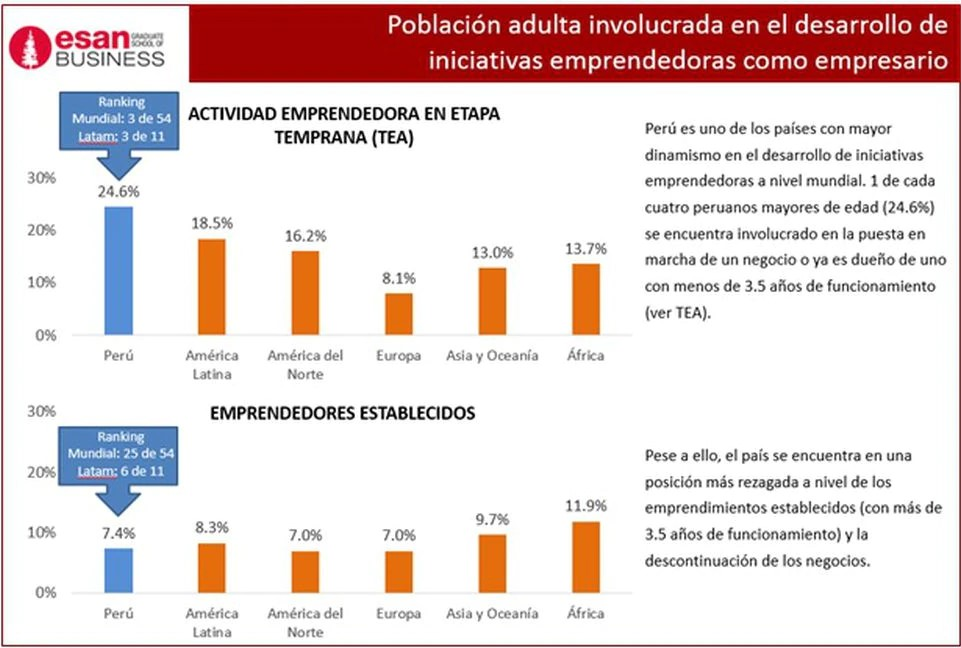
\includegraphics[width=0.65\textwidth]{1/figures/cuadro_esan.jpg}
		\caption[Resultados y ratios obtenidos en la encuesta por GEM y ESAN]{Resultados y ratios obtenidos en la encuesta por GEM y ESAN.\\
		Fuente: \cite{cr_gestion2018emprend}. \textit{Perú es el tercer país con mayor cantidad de emprendimientos en fase temprana a nivel mundial}.}
		\label{1:fig}
	\end{center}
\end{figure}

Los resultados desfavorables tienen como base el ecosistema poco beneficioso para los emprendimientos que permitan establecerse en su entorno nacional, con condiciones asociadas al acceso de financiamiento, políticas gubernamentales que alienten la implementación de Innovación y Desarrollo en las empresas, acceso a infraestructura física y asesoría a nivel comercial y profesional, como sostiene el investigador del equipo GEM Perú Carlos Guerrero \parencite{cr_gestion2018emprend}. De acuerdo con la \cite{cr_aep2018emprend}, en la región solo se invierte el 1.5\% del PIB en actividades de ciencia, tecnología e innovación, y las limitaciones son dadas por barreras burocráticas ejercidas por el Gobierno y el sector privado. Otras razones que representan barreras para emprender son: la falta de conocimientos en la iniciación de un negocio, su tramitación, la fuente de financiamiento del proyecto o búsqueda de inversionistas, la cultura, la escasa difusión de las ideas que fomenten el emprendimiento y la falta de red de contactos \parencite{cr_sandoval_barreras}.

Ante estas limitaciones, en la actualidad muchos emprendedores se ven forzados a mostrar sus proyectos al público en la Internet con el fin de captar personas interesadas en ayudarlos en el financiamiento de estos. Por ello, se han creado plataformas web con el fin de permitir la interacción entre los proyectos publicados en un determinado tiempo, el cual puede variar entre 30 y 120 días, y la comunidad en general que desee colaborar con una cantidad de dinero para su financiamiento. El sitio web solo servirá para mostrar los proyectos presentados a detalle por los creadores y la promoción de estos al público. La idea es que, al término de este plazo de tiempo, el proyecto sea financiado y se logre convertir en una realidad. A esta práctica se le conoce como crowdfunding \parencite{cr_uc_crowdfunding}.

En Latinoamérica, son muy pocos los países los que se han incorporado en el crowdfunding, entre los principales se destacan Chile, México, Argentina y Brasil. Sin embargo, aquí el modelo funciona distinto que en los países de Norteamérica y Europa debido a la diferencia cultural y resistencia a su implementación por la poca confianza en el éxito de los proyectos. Por ejemplo, se encontró en dichos países que los proyectos audiovisuales, a pesar de encontrarse en desventaja que en sus pares europeos y norteamericanos, se estrenaron 4,135 títulos extranjeros en la región iberoamericana frente a 791 propios, de los cuales 162 fueron obras brasileñas y 131, argentinas, en el año 2015. Algunos de los factores principales fueron el apoyo de sus gobiernos, la masificación de las comunicaciones digitales y por ende, la participación activa de usuarios en redes sociales y el papel protagónico que toma el crowdfunding para apoyar estos proyectos (22,179 proyectos financiados con éxito en Kickstarter con más de 1 millón de dólares de recaudación en el 2017) \parencite{cr_lopezgolan2017crowdfunding}. Asimismo, en los últimos años se decidió seguir una manera muy similar a los modelos de Estados Unidos, basados en la creación de campañas de un emprendedor para obtener fondos para sus ideas con la moneda norteamericana pero limitados a las leyes económicas de cada país \parencite{cr_sl_crowdfundlatam}. En el caso del Perú, el crowdfunding existe y es apoyado por universidades y organizaciones sin fines de lucro, cuyo objetivo es generar empresas comerciales que aumenten la calidad de vida en la comunidad, además de convertir a las personas en socios financieros \parencite{cr_fernandezbedoya2020colecoperu}. Esta actividad es parte de uno de los 4 grupos básicos de economía colaborativa: el financiamiento colaborativo \parencite{cr_stokes2014coleco}.

Kickstarter e Indiegogo figuran entre los sitios web más conocidos de crowdfunding. El primero, desde su inicio en 2009, es una plataforma de financiamiento de proyectos creativos de todo tipo, los cuales incluyen películas, juegos, música, arte, diseño y tecnología. Actualmente, se han registrado más de 162 mil proyectos realizados, 16 millones de contribuyentes y 4,3 miles de millones de dólares fondeados \parencite{cr_kickstarter_about}. Utiliza un modelo de financiamiento llamado “todo o nada”, el cual consiste en que si un proyecto no alcanza su meta de financiamiento en un determinado plazo de tiempo, no se realiza ninguna transacción de fondos \parencite{cr_kickstarter_founding}. Si bien los patrocinadores apoyan estos proyectos por motivos personales y distintos para hacerlos realidad, ellos no obtienen la propiedad o los ingresos de los proyectos que financian, sino que los creadores conservan la totalidad de su trabajo \parencite{cr_kickstarter_press}.

De todas las categorías, los proyectos tecnológicos alcanzaron el ratio más bajo (20\%) al 2019, como se aprecia en la Figura \ref{1:fig2}.
\begin{figure}[h]
	\begin{center}
		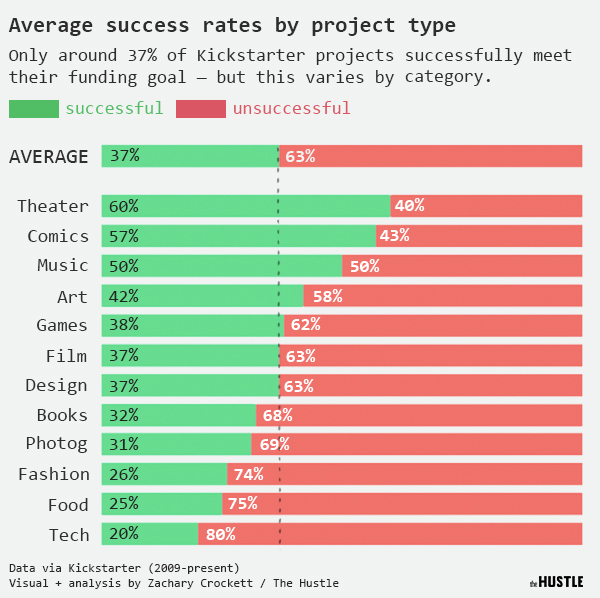
\includegraphics[width=0.55\textwidth]{1/figures/kickstarter_success_rate_2009_2019.jpg}
		\caption[Ratio de éxito de proyectos en Kickstarter desde 2009 hasta 2019 (Febrero)]{Ratio de éxito de proyectos en Kickstarter desde 2009 hasta 2019 (Febrero).\\
		Fuente: \cite{cr_hustle2019successrate}. \textit{What are your chances of successfully raising money on Kickstarter?}}
		\label{1:fig2}
	\end{center}
\end{figure}

Además de este problema, en general muchas veces las campañas fracasan por los valores incorrectos que toman sus variables, desde el contenido de la publicación hasta la comunicación de parte de los creadores con los patrocinadores. Es decir, el factor incertidumbre se vincula con la campaña cuando esta no resulta lo suficientemente atractiva por la ausencia de características que sí presentan los proyectos que fueron financiados.

Existen estudios previos para predecir la probabilidad de éxito de financiamiento para este tipo de proyectos utilizando técnicas de Aprendizaje Automático y Profundo. Sin embargo, la mayoría de los modelos predictivos entrenan usando solo una modalidad o utilizando la data de todas las categorías, originando una generalización en base al ratio global de éxito. Para la actual investigación, se implementó un modelo bajo un enfoque distinto y considerando solamente a proyectos de tecnología.

\section{Formulación del Problema}
Para la formulación de los problemas de la presente investigación, se elaboró un «árbol de problemas» (véase Anexo \ref{anexo1}).

\subsection{Problema General}
PG: \newcommand{\ProblemaGeneral}{
¿Es posible predecir el estado de financiamiento de proyectos de tecnología en sitio web de crowdfunding Kickstarter mediante un modelo de Aprendizaje Profundo Multimodal?
}
\ProblemaGeneral
\subsection{Problemas Específicos}
\newcommand{\Pbone}{
¿Qué alternativas se proponen en los trabajos previos para seleccionar características y desarrollar el marco de trabajo de la investigación?
}
\newcommand{\Pbtwo}{
¿Qué condiciones técnicas factibles de las propuestas de la literatura existen en el ambiente de desarrollo para implementar las características del modelo de Aprendizaje Profundo Multimodal?
}
\newcommand{\Pbthree}{
¿Cuál es el impacto que generarán las características consideradas en el desarrollo del modelo de Aprendizaje Profundo Multimodal?
}
\newcommand{\Pbfour}{
¿Qué alternativas analíticas existen para ayudar a los emprendedores y creadores de proyectos de tecnología en la toma de decisiones y estrategias de sus campañas?
}

\begin{itemize}
	\item PE1: {\Pbone}
	\item PE2: {\Pbtwo}
	\item PE3: {\Pbthree}
	\item PE4: {\Pbfour}
\end{itemize}

\section{Objetivos de la Investigación}
Para la formulación de los objetivos de la presente investigación, se elaboró un «árbol de objetivos» (véase Anexo \ref{anexo2}) 
\subsection{Objetivo General}
OG: \newcommand{\ObjetivoGeneral}{
Predecir el estado de financiamiento de proyectos de tecnología en sitio web de crowdfunding Kickstarter mediante modelo de Aprendizaje Profundo Multimodal.
}
\ObjetivoGeneral
\subsection{Objetivos Específicos}
\newcommand{\Objone}{
Analizar las alternativas propuestas en los trabajos previos para seleccionar características y desarrollar el marco de trabajo de la investigación.
}
\newcommand{\Objtwo}{
Evaluar la factibilidad técnica del ambiente de desarrollo para las características del modelo de Aprendizaje Profundo Multimodal bajo las condiciones de las propuestas de la literatura.
}
\newcommand{\Objthree}{
Examinar el impacto de las características consideradas en el desarrollo del modelo de Aprendizaje Profundo Multimodal.
}
\newcommand{\Objfour}{
Implementar una herramienta analítica en tiempo real para ayudar a los emprendedores y creadores de proyectos de tecnología en la toma de decisiones y estrategias de sus campañas.
}

\begin{itemize}
	\item OE1: {\Objone}
	\item OE2: {\Objtwo}
	\item OE3: {\Objthree}
	\item OE4: {\Objfour}
\end{itemize}

\section{Hipótesis}

\subsection{Hipótesis General}
HG: \newcommand{\HipotesisGeneral}{
	El modelo de Aprendizaje Profundo Multimodal predecirá el estado de financiamiento de proyectos de tecnología en sitio web de crowdfunding Kickstarter.
}
\HipotesisGeneral
\subsection{Hipótesis Específicas}
\newcommand{\Hone}{
El análisis de las alternativas propuestas en los trabajos previos influirá en la selección de características y desarrollo del marco de trabajo de la investigación.
}
\newcommand{\Htwo}{
La factibilidad técnica del ambiente de desarrollo para las características del modelo de Aprendizaje Profundo Multimodal determinará la aplicabilidad de las condiciones de las propuestas de la literatura.
}
\newcommand{\Hthree}{
El modelo de Aprendizaje Profundo Multimodal se verá afectado por las características consideradas en su desarrollo.
}
\newcommand{\Hfour}{
La herramienta analítica implementada ayudará en tiempo real a los emprendedores y creadores de proyectos de tecnología en la toma de decisiones y estrategias de sus campañas.
}

\begin{itemize}
	\item HE1: \Hone
	\item HE2: \Htwo
	\item HE3: \Hthree
	\item HE4: \Hfour
\end{itemize}

Los problemas, objetivos e hipótesis descritas anteriormente se encuentran alineados en la Matriz de Consistencia del Anexo \ref{anexo3}. Además, los objetivos específicos se formularon a partir de una lluvia de ideas luego de examinar los objetivos planteados en los antecedentes, cuyo detalle e item de referencia se encuentra en el Anexo \ref{anexo5}.

\section{Justificación de la Investigación}

\subsection{Teórica}
Esta investigación se realizó con la finalidad de aportar al conocimiento existente del problema de la predicción del estado de financiamiento de un proyecto en plataformas de crowdfunding como Kickstarter, pero considerando solo proyectos de la categoría Tecnología, cuyo ratio de éxito de 20\% la clasifica como la más baja de todas, criterio que también se menciona en la literatura por \cite{pr_lee2018contentDL}.

Para ello, el nuevo aporte aplicado a la investigación fue la implementación de un modelo de Aprendizaje Profundo Multimodal utilizando la información de la sección principal de la campaña (metainformación y descripción) y los comentarios de los patrocinadores como resultado de la interacción entre ellos y los creadores. Esta nueva perspectiva considera las 3 modalidades más utilizadas en los antecedentes bajo un modelo que solo fue desarrollado en 1 antecedente por \cite{pr_cheng2019deeplearning}, el cual utilizó solo modalidades de la sección principal (metainformación, descripción e imagen del proyecto).

\subsection{Práctica}
Muchos trabajos previos analizados en la literatura plantearon distintas soluciones para resolver el mismo problema. Sin embargo, a pesar de que sus resultados en su mayoría alcanzaron niveles de predicción por encima a los esperados por los autores, menos de la mitad (8 de los 18 antecedentes mencionados) llegaron a ejecutar la fase de Despliegue, es decir, no fueron puestos en producción para ser utilizados por otros usuarios, o se mencionaron que se convertiría en una tarea para trabajos a futuro.

Al culminar esta invesigación, se podrá utilizar el prototipo de un sistema que integra el modelo propuesto, el cual funciona en tiempo real capturando la información de las variables solamente recibiendo como entrada la URL del proyecto, con la finalidad de poder ser una herramienta analítica de ayuda en la toma de decisiones a emprendedores que buscan financiar sus proyectos de tecnología en Kickstarter. La retroalimentación será recíproca entre el usuario y el prototipo, ya que en la primera iteración, el creador tendrá una idea inicial del resultado de éxito de financiamiento que tendrá su campaña de acuerdo a la información actual presente en sus variables, y ante una respuesta adversa, podrá realizar las modificaciones respectivas en las modalidades entrenadas que tiene acceso (metainformación y descripción) para ejecutar nuevamente el prototipo, que ahora hará la predicción a partir de nuevos datos, de forma indefinida. De esta manera, se logrará crear una campaña más atractiva para los patrocinadores.

\subsection{Metodológica}
La implementación del modelo propuesto ayudará a los emprendedores y creadores a evaluar las campañas de sus proyectos a partir de la información vigente que sea capturada en tiempo real por el prototipo para predecir el estado de financiamiento.

Para ello, se utilizaron técnicas de Aprendizaje Profundo y Procesamiento de Lenguaje Natural entrenados con un conjunto de datos compuesto por 3 modalidades de proyectos en Kickstarter que fueron generados luego de un proceso de recolección de datos.

\section{Delimitación del Estudio}

\subsection{Espacial}
Para la presente investigación, se consideraron proyectos de tecnología de distintas ciudades y países, mayoritariamente del territorio de los Estados Unidos. Sin embargo, la información textual (descripción y comentarios) para la fase de entrenamiento solo se tómo en cuenta palabras en inglés.

\subsection{Temporal}
El periodo de tiempo abarcará desde el año 2009, fecha en el cual se tiene registrado los primeros conjuntos de datos de proyectos en Kickstarter hasta el mes de agosto del año 2019, últimos registros descargados hasta el inicio del presente trabajo.

\subsection{Conceptual}
Esta investigación se orientará en la implementación de un modelo que logre predecir si un proyecto de tecnología en el sitio web de crowdfunding Kickstarter será financiado o no. Para ello, se valió del uso de herramientas de Aprendizaje Profundo y Procesamiento de Lenguaje Natural para desarrollar los modelos de acuerdo a sus modalidades respectivas, así como el Aprendizaje Profundo Multimodal para consolidar estos conceptos.
%\chapter{Marco Teórico}
\section{Antecedentes de la investigación}
\subsection{\citetitle{pr_contreras2021modelwlan}}
La predicción del éxito o fracaso de las ubicaciones de puntos de acceso interior en diferentes planos utilizando conjuntos de datos con estructuras similares a la del presente trabajo se abordará a continuación en esta sección. En cada uno se describen el problema y su propósito, la metodología utilizada, las técnicas empleadas y los resultados.

\cite{pr_contreras2021modelwlan} publicaron el modelo de optimización  \citetitle{pr_contreras2021modelwlan} para el departamento de Investigación e Innovación en Ingenierías de la Universidad Simón Bolívar.

Debido a su movilidad y bajo costo, la demanda de redes inalámbricas, particularmente WLAN, ha aumentado significativamente. Para que estas redes inalámbricas funcionen en hogares, oficinas y escuelas, los puntos de acceso (AP) son necesarios. La ubicación y densidad de los AP tienen un impacto en la cobertura y la calidad de la señal. Para mejorar la eficiencia y la cobertura de la red, este artículo propone un modelo de optimización para la ubicación de AP en interiores que utiliza el modelo de propagación Log-Normal Shadowing Path Loss.

El desarrollo del modelo de optimización incluyó una serie de pasos importantes: se utilizó el modelo de propagación Log-Normal Shadowing Path Loss para estimar el radio de cobertura y la probabilidad de corte de la señal utilizando dimensiones del escenario, frecuencia y condiciones ambientales; se implementó un pseudocódigo para calcular el radio de cobertura y la probabilidad de corte de la señal para las bandas de 2,4 GHz y 5 GHz; y se diseñó una técnica específica para determinar la ubicación óptima de los AP dentro de una construcción, considerando la probabilidad de corte, la sensibilidad de recepción y otros parámetros técnicos.

Los resultados del modelo sugerido demostraron una mejora significativa en la identificación de las áreas de cobertura y la probabilidad de corte. En particular, se descubrió que la banda de 2.4 GHz cubre un mayor área de cobertura en comparación con la banda de 5 GHz, pero también se observó que tiene una mayor probabilidad de interferencia. La técnica permitió el cálculo de los radios de cobertura apropiados y la mejora de la ubicación geográfica de los AP, lo que permitió maximizar la cobertura y reducir las zonas de silencio. Las tablas y los gráficos que muestran la relación entre la distancia y la potencia de la señal describieron los parámetros específicos para cada banda de frecuencia y tipo de entorno.

El modelo de optimización para la ubicación de puntos de acceso en redes WLAN en ambientes interiores demostró ser efectivo para aumentar la cobertura y reducir la probabilidad de corte de señal como se ilustra en la Figura 3. Los algoritmos y metodologías creados ofrecen una herramienta útil para diseñar y desplegar redes WLAN de manera eficiente. Este modelo debería ser utilizado en futuras investigaciones y aplicaciones prácticas para mejorar la calidad y el rendimiento de las redes inalámbricas, especialmente en entornos con alta densidad de usuarios y dispositivos.

\begin{figure}[!ht]
	\begin{center}
		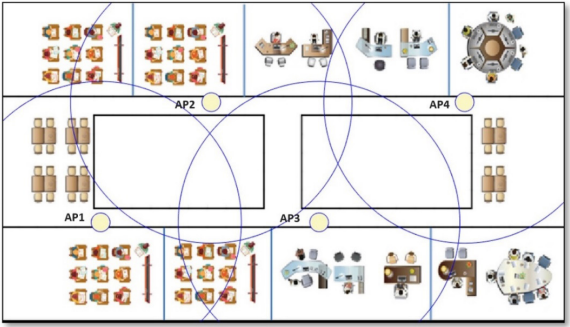
\includegraphics[width=0.80\textwidth]{2/figures/contreras2021.png}
		\caption[Diagrama de cobertura y ubicación de AP]{Diagrama de cobertura y ubicación de AP.\\
			Fuente: \cite{pr_contreras2021modelwlan}. \citetitle{pr_contreras2021modelwlan}. (p. 14)}
		\label{2:fig111}
	\end{center}
\end{figure}

\subsection{\citetitle{pr_alathari2023optaps}}
Según el acta de la conferencia "TInternational Conference on Computational Science and Technology", que se llevó a cabo en 2022, \cite{pr_alathari2023optaps} publicaron el artículo conocido como \citetitle{pr_alathari2023optaps}, "Optimización de la ubicación de puntos de acceso en comunicaciones interiores" en español.

El estudio presenta un modelo de optimización para la ubicación de puntos de acceso (AP) en redes inalámbricas. Utilizando técnicas sofisticadas de algoritmos genéticos y simulaciones de Monte Carlo, el objetivo principal es maximizar la cobertura y minimizar la interferencia. La necesidad creciente de mejorar la eficiencia de las redes inalámbricas en entornos de alta densidad es el tema de esta investigación.

La técnica utilizada consta de numerosos pasos cruciales. Primero, se recopilan datos sobre la distribución del espacio y la cobertura. Después, se utiliza un algoritmo genético para crear las ubicaciones iniciales potenciales de AP. Se utilizan simulaciones de Monte Carlo para evaluar la efectividad de estas ubicaciones en términos de cobertura y minimización de interferencia. Se siguen estos pasos hasta llegar a la configuración de AP ideal.

Comparado con las técnicas convencionales, los resultados muestran una mejora significativa en la cobertura de la red y una reducción en la interferencia que se puede observar en la Figura 4. Se logró aumentar la cobertura en un 25 \% y disminuir la interferencia en un 15 \%. Estos hallazgos se comprobaron en un entorno simulado que emulaba las condiciones de una red inalámbrica de alta densidad real.

\begin{figure}[!ht]
	\begin{center}
		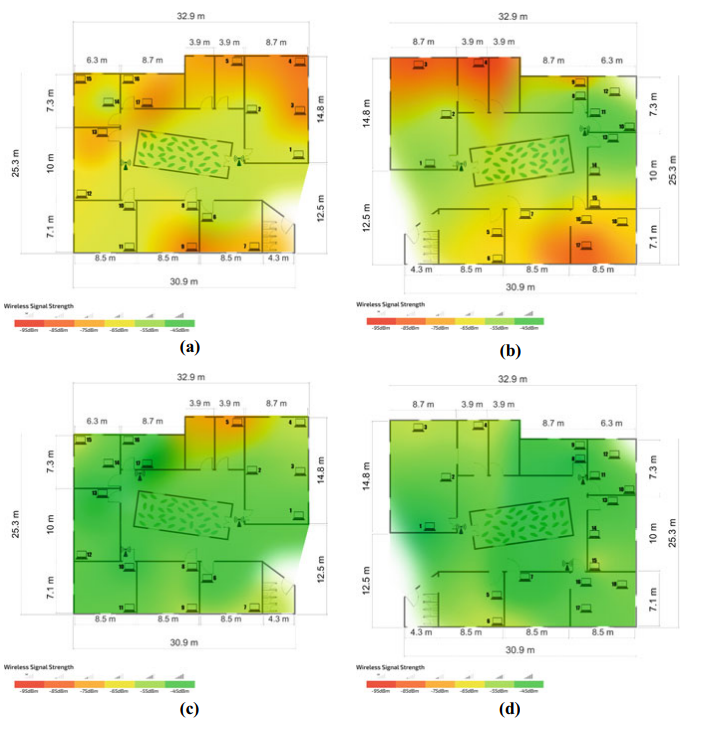
\includegraphics[width=0.75\textwidth]{2/figures/alathari2023.png}
		\caption[Un mapa de calor que describe la intensidad de la señal recibida antes y después. a Área de cobertura de la señal para los puntos de acceso de la izquierda, b Área de cobertura de la señal para los puntos de acceso de la derecha, c Área de cobertura de la señal para los puntos de acceso de la izquierda, d Área de cobertura de la señal para los puntos de acceso de la derecha.]{Un mapa de calor que describe la intensidad de la señal recibida antes y después. a Área de cobertura de la señal para los puntos de acceso de la izquierda, b Área de cobertura de la señal para los puntos de acceso de la derecha, c Área de cobertura de la señal para los puntos de acceso de la izquierda, d Área de cobertura de la señal para los puntos de acceso de la derecha.\\
		Fuente: \cite{pr_alathari2023optaps}. \citetitle{pr_alathari2023optaps}. (p. 11)}
		\label{2:fig112}
	\end{center}
\end{figure}

\subsection{\citetitle{pr_ketkhaw2019deepl}}
\cite{pr_ketkhaw2019deepl}  publicaron la investigación \citetitle{pr_ketkhaw2019deepl}, en español "Predicción de la ubicación de puntos de acceso no autorizados basada en redes neuronales profundas", se publicó en el journal tailandés "Journal of Mobile Multimedia" en 2022.

El objetivo del estudio es desarrollar un método llamado LPRAP que utiliza redes neuronales profundas para predecir la ubicación de puntos de acceso no autorizados en redes inalámbricas locales. La detección y localización precisa de estos RAPs es esencial para garantizar la seguridad de las redes y proteger la información confidencial de posibles amenazas.

Los dos mecanismos principales del proceso LPRAP son la detección de RAPs y la predicción de su ubicación. Para determinar la intensidad de la señal recibida (RSSI) en cada subárea, se recopila un conjunto de marcos de balizas en la detección de RAP. Posteriormente, se clasifica la ubicación de los RAPs utilizando un espacio de características de 81 dimensiones. En cuanto a la predicción de ubicación, se utiliza la precisión de la predicción de ubicación para evaluar el rendimiento del esquema propuesto comparándolo con otros algoritmos de aprendizaje automático como SVM, KNN, Naive Bayes y MLP.

Los resultados del experimento muestran que LPRAP supera a todos los demás algoritmos de aprendizaje automático evaluados. La precisión de la predicción de la ubicación de los RAPs aumenta significativamente con el aumento del número de subáreas. Por ejemplo, LPRAP logra una precisión de predicción del 88,31\% para 3 subáreas, lo que demuestra su capacidad para detectar y encontrar RAPs en entornos de redes inalámbricas como se puede observar en la Figura 6.

\begin{figure}[!ht]
	\begin{center}
		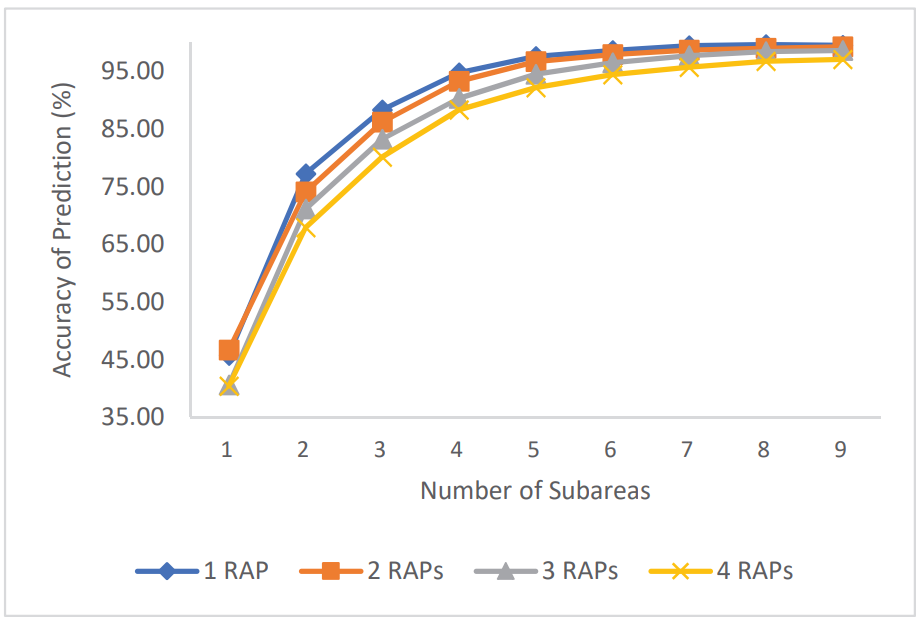
\includegraphics[width=0.75\textwidth]{2/figures/ketkha2022.png}
		\caption[Precisión de la predicción en función del número de subzonas para la predicción de la ubicación de 1 a 4 RAP.]{Precisión de la predicción en función del número de subzonas para la predicción de la ubicación de 1 a 4 RAP.\\
		Fuente: \cite{pr_ketkhaw2019deepl}. \citetitle{pr_ketkhaw2019deepl}. (p. 13)}
		\label{2:fig114}
	\end{center}
\end{figure}

\subsection{\citetitle{pr_nauata2021housegan}}
\cite{pr_nauata2021housegan} ,en la conferencia "2021 IEEE/CVF Conference on Computer Vision and Pattern Recognition (CVPR)", que tuvo lugar en Nashville, Tennessee, Estados Unidos en el año 2021, publicaron un artículo titulado \citetitle{pr_nauata2021housegan}, en español se traduce como "House-GAN++: Generative Adversarial Layout Refinement Network hacia un agente computacional inteligente para arquitectos profesionales".

Para la generación automatizada de planos de planta, se sugiere una red generativa rival de refinamiento de diseño de planos de planta (House-GAN++). El sistema recibe un diagrama de burbujas que muestra las conexiones funcionales entre las habitaciones y, como salida, crea un plano de planta realista.

Como se muestra en la Figura 7, la arquitectura sugerida integra una GAN relacional con restricciones de grafo y una GAN condicional. El generador itera el diseño antes de convertirlo en la siguiente restricción de entrada. Cada componente recibe una máscara de segmentación de la verdad fundamental con una probabilidad aleatoria durante el entrenamiento (condicionamiento GT por componente).

\begin{figure}[!ht]
	\begin{center}
		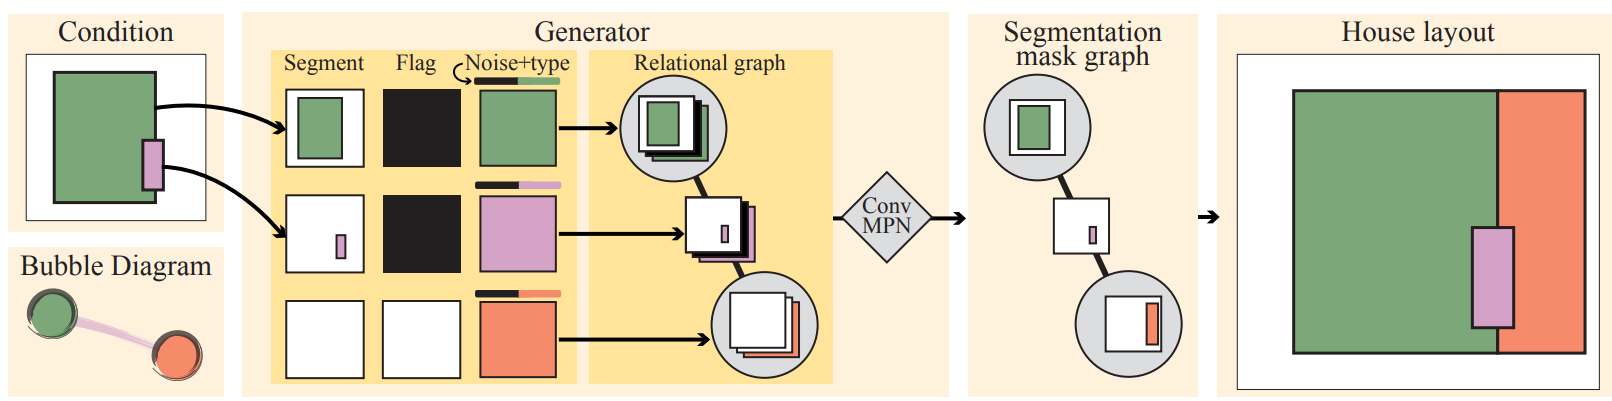
\includegraphics[width=0.8\textwidth]{2/figures/nauata2021.png}
		\caption[La arquitectura se basa en un GAN relacional. Se puede especificar una máscara de segmentación 2D adicional para cada habitación/puerta como condición de entrada, lo que permite un refinamiento iterativo del diseño.]{La arquitectura se basa en un GAN relacional. Se puede especificar una máscara de segmentación 2D adicional para cada habitación/puerta como condición de entrada, lo que permite un refinamiento iterativo del diseño.\\
		Fuente: \cite{pr_nauata2021housegan}. \citetitle{pr_nauata2021housegan}. (p. 3)}
		\label{2:fig115}
	\end{center}
\end{figure}

El sistema sugerido supera ampliamente los enfoques del estado del arte actuales en las tres métricas estándar de realismo, diversidad y compatibilidad. En un estudio de usuarios con arquitectos profesionales, el sistema obtuvo puntajes de realismo de -0.7 para los métodos comparativos y puntajes de 0.5 para el sistema propuesto en la tarea más difícil de generar planos de 8 habitaciones. Como se muestra en la Figura 8, la distancia de edición de gráficos (compatibilidad) aumenta de 11.8 para el estado del arte a 6.5 para el sistema propuesto en planos de 8 habitaciones.

\begin{figure}[!ht]
	\begin{center}
		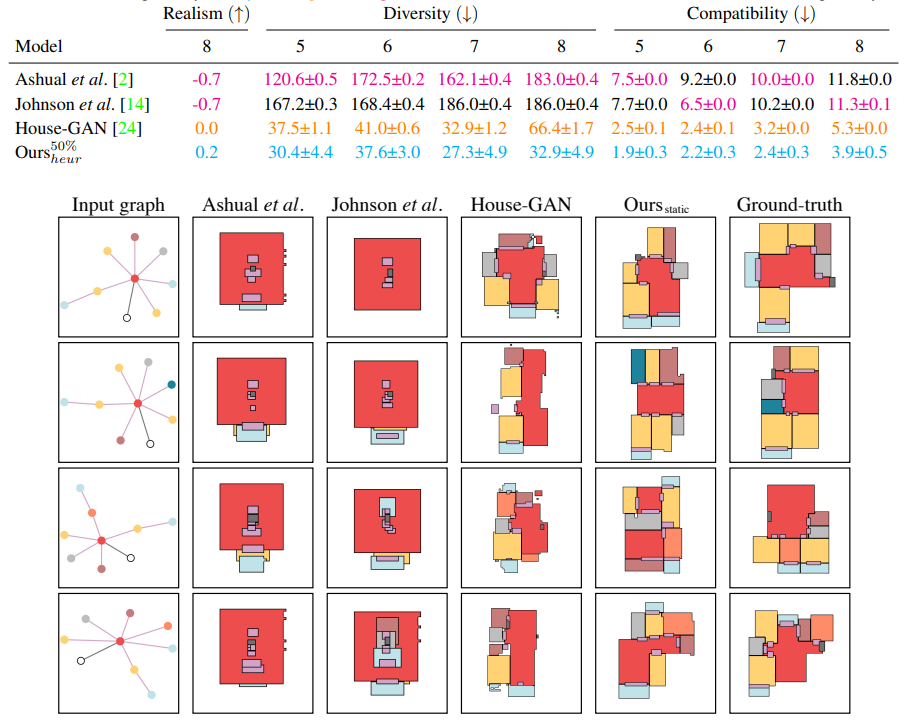
\includegraphics[width=1.1\textwidth]{2/figures/nauata2021_2.png}
		\caption[Evaluación del realismo. Se muestra un diseño generado para cada diagrama de burbujas de entrada]{Evaluación del realismo. Se muestra un diseño generado para cada diagrama de burbujas de entrada.\\
			Fuente: \cite{pr_nauata2021housegan}. \citetitle{pr_nauata2021housegan}. (p. 6)}
		\label{2:fig116}
	\end{center}
\end{figure}

\subsection{\citetitle{pr_cai2023precisewifi}}
\cite{pr_cai2023precisewifi} publicaron un artículo que se llamaba \citetitle{pr_cai2023precisewifi}, el término se traduce al español como "Posicionamiento WiFi preciso en el interior mediante algoritmos de aprendizaje profundo" para la revista científica "ArXiv:2307.02011v" publicada en 2023.

Este artículo presenta una nueva estrategia para el posicionamiento en interiores que emplea tecnología WiFi. Para mejorar la precisión del posicionamiento en comparación con el enfoque tradicional basado únicamente en RSSI, se recomienda utilizar una combinación de mediciones de la Intensidad de la Señal Recibida (RSSI) y el Ángulo de Llegada (AoA).

La metodología se compone de tres pasos principales: 1) Usando puntos de referencia, crear modelos de posicionamiento basados en RSSI y el método híbrido RSSI-AoA; 2) Entrenar los modelos utilizando varios algoritmos de aprendizaje profundo, como BPNN, RBF y CNN; 3) Probar el rendimiento de los modelos y calcular los errores en tres entornos de prueba diferentes: un salón de clases grande, un salón de clases pequeño y un salón de clases pasillo.

Independientemente del algoritmo de aprendizaje profundo utilizado y del entorno de prueba, los resultados muestran que el método híbrido RSSI-AoA tiene un error medio absoluto (MAE) más pequeño que el método basado únicamente en RSSI. Por ejemplo, el MAE del método híbrido con CNN es inferior a 300 mm en un salón de clases grande, mientras que el MAE del método basado en RSSI con CNN es inferior a 400 mm. Como se muestra en la Figura 9, el algoritmo CNN supera a BPNN y RBF en ambos modelos de posicionamiento.

\begin{figure}[!ht]
	\begin{center}
		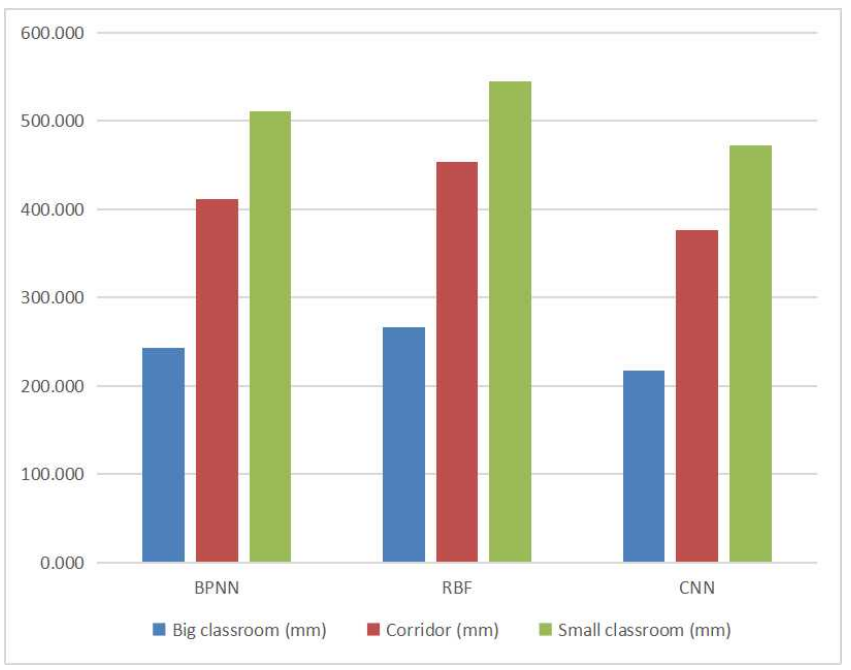
\includegraphics[width=0.90\textwidth]{2/figures/cai2023.png}
		\caption[Los MAE del modelo híbrido de posicionamiento]{Los MAE del modelo híbrido de posicionamiento.\\
			Fuente: \cite{pr_cai2023precisewifi}. \citetitle{pr_cai2023precisewifi}. (p. 26)}
		\label{2:fig117}
	\end{center}
\end{figure}

\subsection{\citetitle{pr_hosseini2023NSGAIIap}}
En el año 2023, la revista "Automation in Construction" publicó \cite{pr_hosseini2023NSGAIIap} publicaron el artículo conocido como \citetitle{pr_hosseini2023NSGAIIap}, "Ubicación óptima de puntos de acceso Wi-Fi basada en NSGA-II para posicionamiento interior: una predicción RSS basada en BIM", según su traducción al español.

Este artículo presenta un método para optimizar la colocación de puntos de acceso Wi-Fi (AP) en interiores utilizando un modelo de propagación de señal calibrado y un algoritmo genético multiobjetivo (NSGA-II).

La técnica consta de varias etapas: 1) Voxelización del modelo BIM del edificio, 2) Muestreo de intensidad de señal recibida (RSS) en puntos de control y verificación, 3) Calibrar el modelo de propagación de señal mediante el método de cuadrados mínimos, 4) Creación de huellas digitales virtuales 3D y 5) Uso de NSGA-II para optimizar la ubicación de los AP Wi-Fi. 

Los resultados demuestran que el método sugerido puede reducir significativamente el número de AP Wi-Fi necesarios sin sacrificar la precisión de la ubicación. La mejor solución encontrada tenía 4 APs y 13 APs, respectivamente, con una mejora en la precisión del posicionamiento del 35.54\% y 44.82\% en comparación con la distribución actual de 6 APs, como se muestra en la Figura 10.

\begin{figure}[!ht]
	\begin{center}
		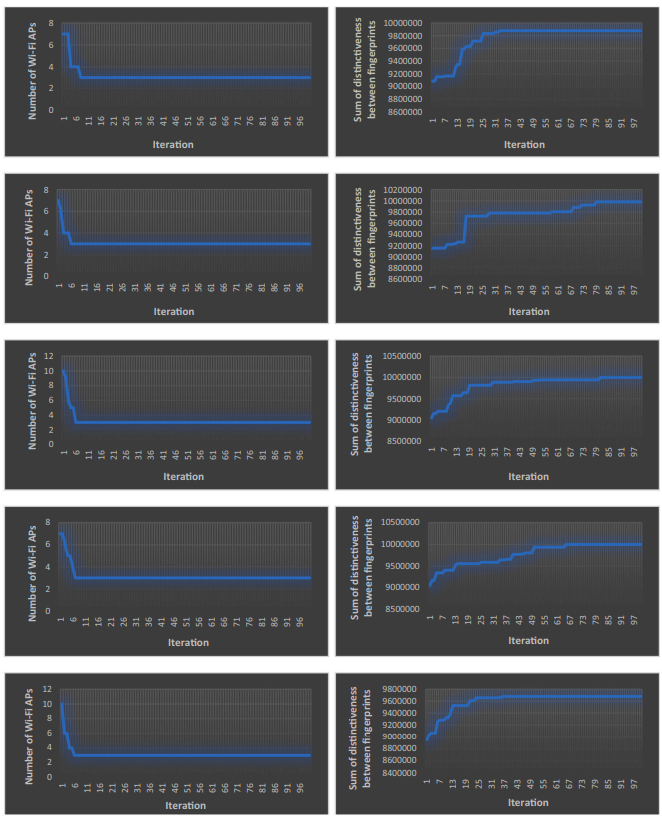
\includegraphics[width=0.75\textwidth]{2/figures/hosseini2023.png}
		\caption[Los resultados de la evaluación de la convergencia del NSGA-II]{Los resultados de la evaluación de la convergencia del NSGA-II.\\
		Fuente: \cite{pr_hosseini2023NSGAIIap}. \citetitle{pr_hosseini2023NSGAIIap}. (p. 16)}
		\label{2:fig118}
	\end{center}
\end{figure}

\subsection{\citetitle{pr_lee2015coverage3d}}
En noviembre del 2015, en la publicación "Computers, Environment and Urban Systems", \cite{pr_lee2015coverage3d} publicaron un artículo que se llamaba \citetitle{pr_lee2015coverage3d}, "Modelización 3D de la ubicación de puntos de acceso Wi-Fi en interiores" en español.

Este documento presenta un modelo de optimización para la ubicación de puntos de acceso (AP) Wi-Fi en un entorno interior de múltiples pisos con el objetivo de maximizar la cobertura de la señal. El modelo utiliza el modelo de sombra log-normal para considerar la atenuación de la señal en tres dimensiones. Esto permite una representación más precisa de la cobertura de la señal en comparación con los métodos tradicionales en dos dimensiones.

El artículo aborda los siguientes puntos importantes: Para estimar la atenuación de la señal en 3D, se define un modelo de propagación de señal log-normal en sombra. El problema de ubicación de AP se identificó como un problema de cobertura de señal máxima (MSCLP), Resolver el MSCLP utilizando un algoritmo de optimización para encontrar las ubicaciones de AP ideales, y finalmente, utilizando esferas que representan la fuerza de la señal en los puntos de demanda para visualizar la cobertura 3D resultante.

El modelo sugerido indica que las ubicaciones de AP ideales se encuentran en varios pisos, con el 70\% de las ubicaciones en los pisos centrales tercero y cuarto. Se logra una cobertura del 98.81\% de los puntos de demanda para una solución con 10 AP sin restricción de capacidad. A medida que se agregan más AP, la fuerza de señal promedio aumenta, pero la tasa de aumento disminuye. La solución propuesta con el mismo número de AP cubre significativamente más puntos de demanda que la solución actual de 117 AP en el edificio de prueba (77.61\% en comparación con 54.63\%). Según el modelo, solo se necesitarían 21 AP sin restricción de capacidad para una cobertura completa, como se muestra en la Figura 11.

\begin{figure}[!ht]
	\begin{center}
		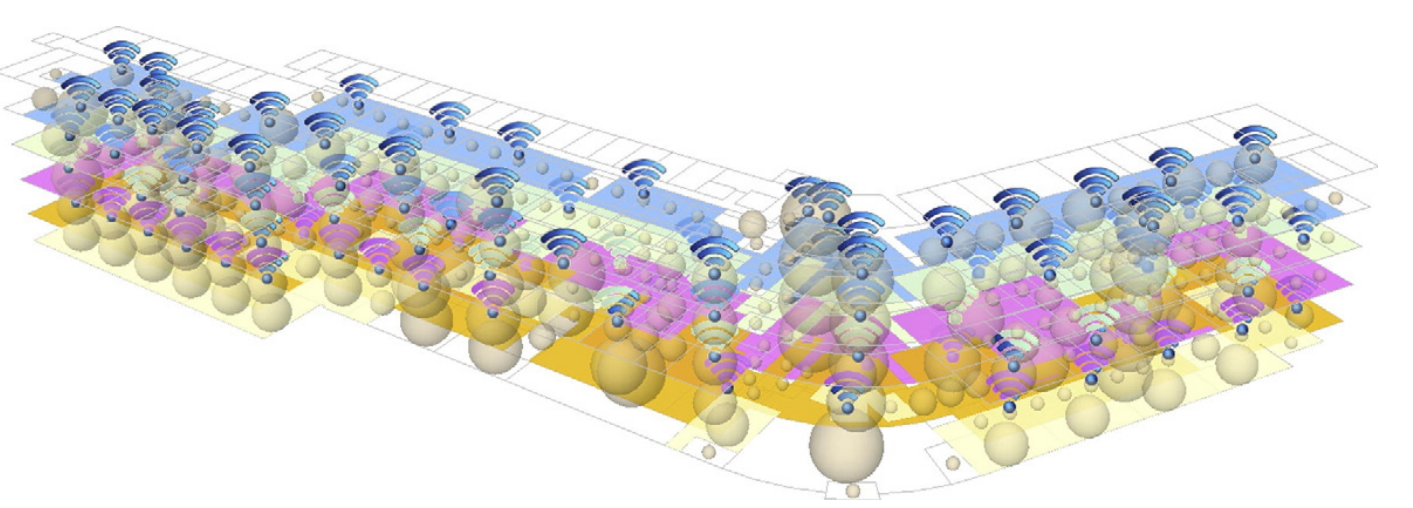
\includegraphics[width=1\textwidth]{2/figures/lee2015.png}
		\caption[Colocación óptima de AP capacitados con demandas ponderadas (p = 117)]{Colocación óptima de AP capacitados con demandas ponderadas (p = 117).\\
		Fuente: \cite{pr_lee2015coverage3d}. \citetitle{pr_lee2015coverage3d}. (p. 9)}
		\label{2:fig119}
	\end{center}
\end{figure}

\subsection{\citetitle{pr_ozerol2023genermass}}
En marzo de 2023, en la revista científica "Architecture and Planning Journal (APJ)", \cite{pr_ozerol2023genermass} publicaron el artículo conocido como \citetitle{pr_ozerol2023genermass}, en español, esto se traduce como "Creación de planes de vivienda colectiva a través de Gans - Un caso en Tokio, Turquía".

El estudio investigó la capacidad de Generative Adversarial Neural Networks (GAN) para crear dibujos arquitectónicos de proyectos de vivienda masiva de TOKI utilizando conjuntos de datos. El objetivo principal fue capacitar al algoritmo HouseGAN para crear tipologías de planos de TOKI actuales y diagramas de burbujas.

En el artículo se explica cómo se multiplicaron planos correlacionados espacialmente con la configuración RGB de 21 tipologías de planos para obtener 157 conjuntos de datos de planos. Estos datos se utilizaron para entrenar al algoritmo de deep learning HouseGAN, que generó imágenes de fondo realistas como salidas del proceso de entrenamiento. El estudio siguió los siguientes pasos: Los diseños arquitectónicos de los proyectos de vivienda masiva de TOKI se utilizaron como conjuntos de datos. Después, se multiplicaron los planos para obtener 157 conjuntos de datos de planos, que se correlacionaron espacialmente con la configuración RGB de 21 tipologías de planos. Posteriormente, se empleó el conjunto de datos generado para entrenar a HouseGAN. Finalmente, los resultados del entrenamiento se convirtieron en imágenes de fondo realistas.

La investigación reveló que la planificación del diseño espacial del algoritmo HouseGAN proporciona diagramas de burbujas y tipologías de planos de TOKI actuales. Como se muestra en la Figura 12, este método permitió crear planos arquitectónicos útiles y realistas para el desarrollo de proyectos de vivienda masiva.

\begin{figure}[!ht]
	\begin{center}
		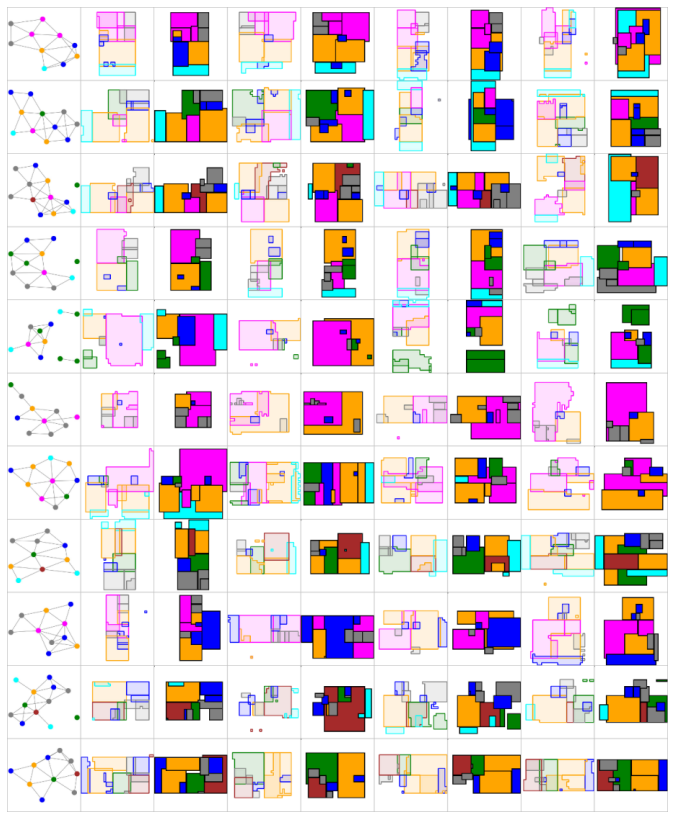
\includegraphics[width=1\textwidth]{2/figures/ozerol2023.png}
		\caption[HouseGAN con LIFULL HOMES Datasets, imágenes generadas por los autores]{HouseGAN con LIFULL HOMES Datasets, imágenes generadas por los autores.\\
		Fuente: \cite{pr_ozerol2023genermass}. \citetitle{pr_ozerol2023genermass}. (p. 10)}
		\label{2:fig120}
	\end{center}
\end{figure}

\subsection{\citetitle{pr_chang2021buildinggan}}
En abril del 2021, en la revista científica "arXiv", \cite{pr_chang2021buildinggan} publicaron el artículo conocido como \citetitle{pr_chang2021buildinggan}, el título "Building-GAN: generación de diseños arquitectónicos volumétricos condicionados por grafos" se traduce al español.

Para mejorar la eficiencia en el diseño volumétrico de edificios en la industria de la arquitectura y la construcción, este artículo presenta un enfoque innovador llamado Building-GAN. Para visualizar los diseños arquitectónicos, se introduce un grafo de voxels tridimensional, así como un generador que incorpora un módulo de punteros cruzados para conectar el grafo de programas y el grafo de voxels.

El artículo detalla los pasos que se deben seguir para crear el modelo Building-GAN. Comienza con la recopilación de datos, que produce un conjunto de datos sintéticos que incluye 120,000 diseños volumétricos de edificios comerciales. Luego se implementa un Grafo Neural Generativo (GNN) de voxels y se crea un grafo de programas jerárquico. Un módulo cruzado basado en punteros también se agrega para conectar los grafos de programas y los voxels.

Los resultados muestran que el modelo propuesto supera significativamente al método anterior, House-GAN, en un estudio de usuarios con 20 arquitectos profesionales, con una puntuación promedio de 0.85 y 0.92, respectivamente. Además, el modelo propuesto obtiene una puntuación promedio de 0.37 en comparación con el modelo Ground Truth, lo que indica que los arquitectos a menudo no pueden distinguir claramente entre el modelo Ground Truth y el modelo propuesto, como se muestra en la Figura 13.

\begin{figure}[!ht]
	\begin{center}
		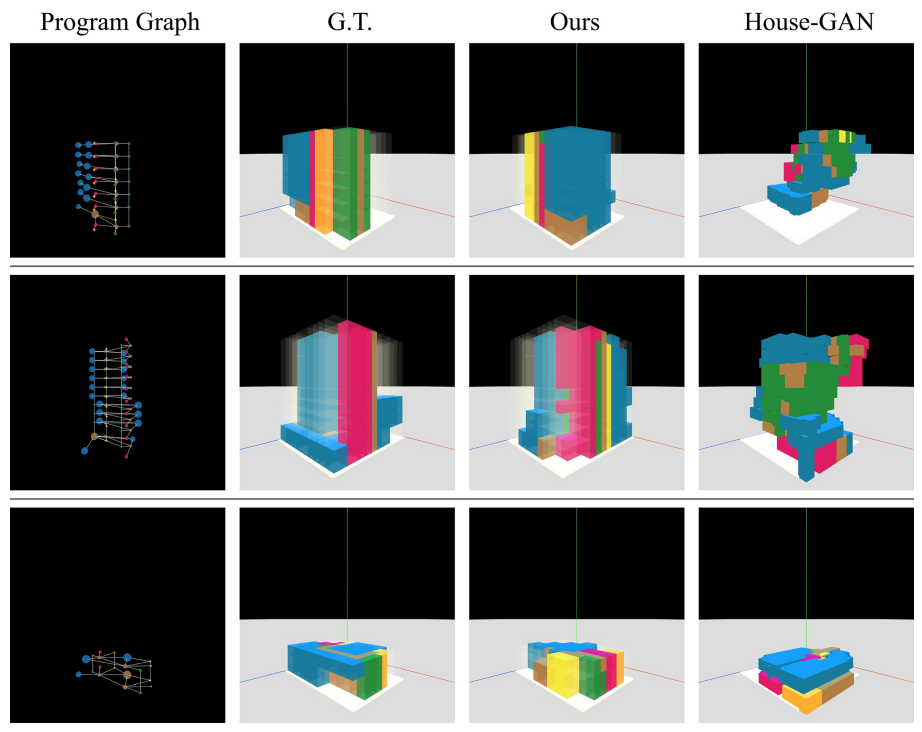
\includegraphics[width=0.7\textwidth]{2/figures/chang2021.png}
		\caption[Para cada gráfico de programa, se generan diseños volumétricos mediante nuestro modelo y mediante House-GAN]{Para cada gráfico de programa, se generan diseños volumétricos mediante nuestro modelo y mediante House-GAN.\\
		Fuente: \cite{pr_chang2021buildinggan}. \citetitle{pr_chang2021buildinggan}. (p. 7)}
		\label{2:fig121}
	\end{center}
\end{figure}

\subsection{\citetitle{pr_chen2020intelhome3d}}
\cite{pr_chen2020intelhome3d} publicaron un artículo que se llamaba \citetitle{pr_chen2020intelhome3d}, en español, se ha traducido como "Inteligente Casa 3D: Diseño automático de casas en 3D solo a partir de descripciones lingüísticas" para la revista científica "arXiv" en 2020.

Este artículo presenta un modelo generativo que utiliza descripciones lingüísticas para diseñar automáticamente planos de casas en tres dimensiones. Dos tareas principales componen el proceso: generar el plano de la planta y la síntesis de las texturas internas.

Los siguientes son los pasos que componen la metodología: representar las descripciones lingüísticas en un grafo estructural utilizando un analizador de escenas de Stanford, utilizando una red neuronal condicional de grafos (GC-LPN) para crear un diseño de planta grueso. Refinar el diseño grueso para crear un plano que incluya puertas y ventanas, Usando una red generativa adversaria condicional a lenguaje (LCT-GAN), se pueden sintetizar las texturas interiores de cada habitación. crear y mostrar la escena 3D completa a partir del plano con texturas.

Los hallazgos indican que el 39,41\% de los diseños creados por el modelo no se distinguían de los creados por humanos en un estudio en el que participaron 20 personas. Además, en evaluaciones cuantitativas, el modelo obtuvo un puntaje de IoU de 0,4765 para la generación de planos y un FID de 27,32 para la síntesis de texturas.

\begin{figure}[!ht]
	\begin{center}
		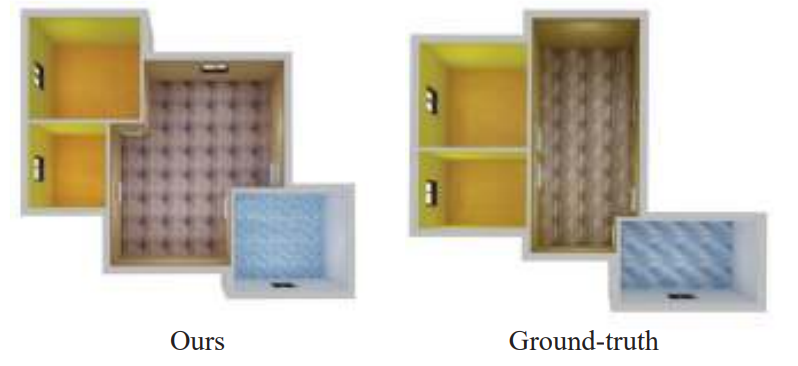
\includegraphics[width=0.73\textwidth]{2/figures/chen2020.png}
		\caption[Comparación de nuestros planos de casas en 3D generados con sus contrapartes reales (hechas por humanos)]{Comparación de nuestros planos de casas en 3D generados con sus contrapartes reales (hechas por humanos).\\
		Fuente: \cite{pr_chen2020intelhome3d}. \citetitle{pr_chen2020intelhome3d}. (p. 8)}
		\label{2:fig122}
	\end{center}
\end{figure}

\subsection{\citetitle{pr_dou2023researchwir}}
\cite{pr_dou2023researchwir} publicaron un artículo que se llamaba \citetitle{pr_dou2023researchwir}, "Investigación sobre cobertura de red inalámbrica para la transformación y actualización de la gestión expositiva con tecnología de inteligencia artificial", según la revista académica internacional "Matemáticas aplicadas y ciencias no lineales" en junio de 2023.

El rápido crecimiento de la inteligencia artificial y la tecnología de comunicación moderna ofrece una oportunidad poderosa para transformar, actualizar y desarrollar una gestión de exposiciones de alta calidad. Sin embargo, es necesario abordar el problema de la cobertura ideal de la red inalámbrica en el área de exposición. Se ha introducido un nuevo algoritmo de inteligencia artificial basado en la optimización de Harris Hawk (HHO) para abordar este problema.

El artículo resuelve el problema de cobertura de la red inalámbrica utilizando un método de optimización multiobjetivo. Primero, el problema de la cobertura se plantea como una función de objetivo que busca maximizar la cobertura y minimizar la redundancia. Como se muestra en la Figura 14, se resuelve este problema utilizando el algoritmo de optimización de Harris Hawk mejorado (IHHO). El IHHO permite una búsqueda eficiente del espacio de soluciones al simular el comportamiento de los halcones de Harris al cazar presas. Además, para inicializar la población, se utiliza un muestreo de hipercubo latino, lo que mejora la diversidad de la población inicial y reduce la probabilidad de convergencia prematura.

\begin{figure}[!ht]
	\begin{center}
		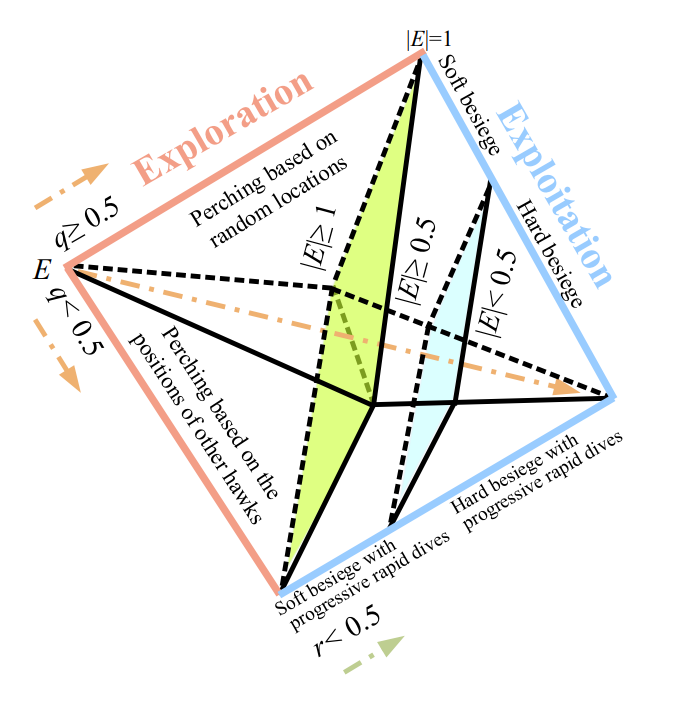
\includegraphics[width=0.5\textwidth]{2/figures/dou2023.png}
		\caption[Estructura de HHO]{Estructura de HHO.\\
		Fuente: \cite{pr_dou2023researchwir}. \citetitle{pr_dou2023researchwir}. (p. 5)}
		\label{2:fig123}
	\end{center}
\end{figure}

Como se muestra en la Figura 15, los resultados de la simulación muestran que el algoritmo de optimización tiene un índice de evaluación integral del 98,03\%, que es superior al del optimizador de enjambre de partículas (PSO) y al algoritmo HHO estándar. Esto demuestra que el algoritmo IHHO sugerido es efectivo para resolver los problemas de cobertura de la red inalámbrica y mejora la cobertura de los nodos más que los métodos de optimización convencionales.

\begin{figure}[!ht]
	\begin{center}
		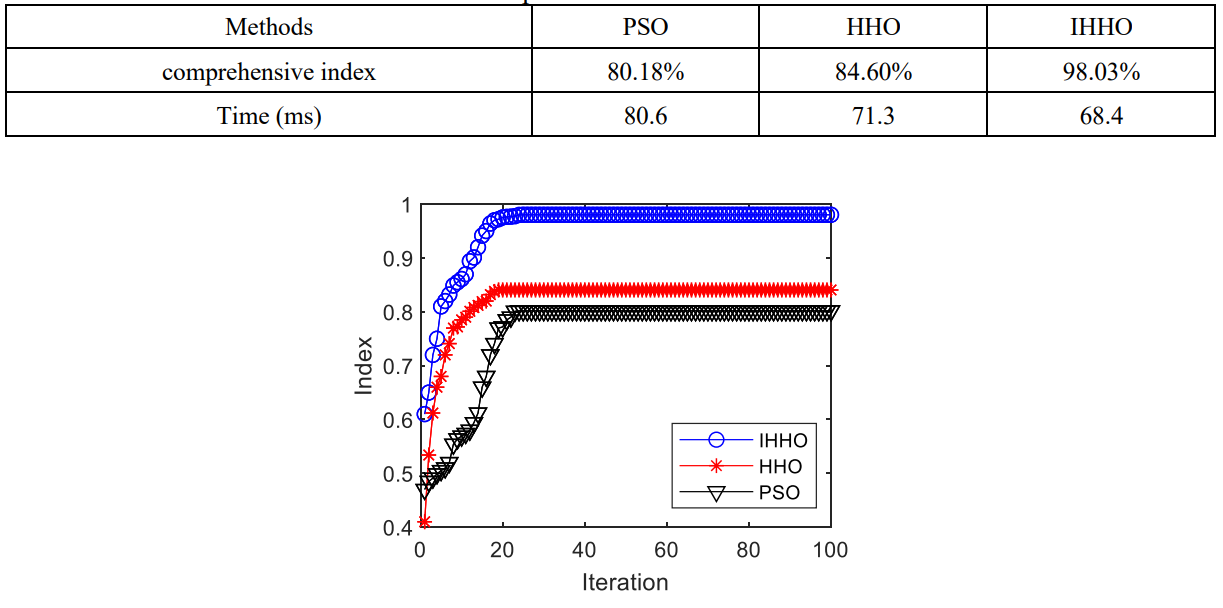
\includegraphics[width=0.5\textwidth]{2/figures/dou2023_2.png}
		\caption[Comparaciones entre los métodos]{Comparaciones entre los métodos.\\
			Fuente: \cite{pr_dou2023researchwir}. \citetitle{pr_dou2023researchwir}. (p. 11)}
		\label{2:fig124}
	\end{center}
\end{figure}
\clearpage

\section{Bases Teóricas}
\subsection{Inteligencia Artificial}

El método racional combina la ingeniería y las matemáticas en base a las "leyes del pensamiento", que se remontan a la antigua Grecia y son influenciadas por filósofos como Aristóteles. Se desarrollaron programas capaces de resolver problemas de lógica en el siglo XIX. Por lo tanto, el objetivo de la inteligencia artificial en el mundo real es desarrollar sistemas inteligentes que tengan estas capacidades. Incluso cuando hay incertidumbre, un "agente racional" actúa para lograr el mejor resultado posible. La inteligencia artificial se basa en una variedad de ciencias, como la ingeniería computacional, la teoría de control, la cibernética, la lingüística, la filosofía, la economía, la psicología, la neurociencia y las matemáticas, según \parencite{bk_russell2004intart}.

Dos investigadores en neurociencia crearon el primer modelo de IA basado en neuronas artificiales en 1943, dando inicio al análisis de la inteligencia artificial. Warren McCulloch y Walter Pitts idearon un modelo que permitía que las neuronas fueran "activadas" o "desactivadas", lo que demostró que una red de neuronas era capaz de realizar cualquier tarea computacional. Posteriormente, Donald Hebb propuso la "regla de aprendizaje hebbiano". John McCarthy, Allen Newell y Herbert Simon desarrollaron un programa capaz de pensar de forma no numérica en el taller de Dartmouth, aunque no se publicó. El término "Inteligencia Artificial" fue acuñado por McCarthy, \parencite{bk_russell2004intart}.

La IA comenzó a entrar en la industria en los años 80, especialmente en grandes empresas de países desarrollados, a través de la investigación en sistemas expertos y el desarrollo de computadoras más poderosas.

\subsection{Aprendizaje Automático}
El aprendizaje automático es una rama de la inteligencia artificial que se centra en técnicas que permiten a las computadoras aprender mediante algoritmos, transformando muestras de datos en programas sin necesidad de programación explícita. \parencite{bk_russell2009intart} describen el aprendizaje automático como una rama de la inteligencia artificial. Estos algoritmos utilizan tecnologías como el procesamiento del lenguaje natural, el aprendizaje profundo y las redes neuronales. Ambos tipos de aprendizaje, supervisado y no supervisado, se basan en lecciones derivadas de datos. El desarrollo de algoritmos que puedan recibir datos de entrada y utilizar análisis estadístico para predecir una salida, que cambia a medida que se adquieren nuevos datos, es la base del aprendizaje automático. \parencite{bk_alpaydin2014ml}

Se puede clasificar en cuatro tipos principales de la siguiente manera según el objetivo que se desea alcanzar mediante el uso de ML:
\begin{itemize}
	\item \textbf{Aprendizaje supervisado}: El aprendizaje supervisado se ganó su nombre porque los científicos de datos actúan como una guía para enseñarle al algoritmo las conclusiones a las que debe llegar. Es similar a la forma en que un estudiante aprende aritmética básica de un maestro. Este tipo de aprendizaje requiere datos etiquetados con las respuestas correctas que se esperan del resultado del algoritmo. Para problemas de clasificación y regresión, el aprendizaje supervisado demostró ser preciso y rápido según \parencite{bk_zambrano2018supnosup}.
	
	Los dos tipos de aprendizaje supervisado son:

	\begin{itemize}
		\item \textbf{La Clasificación}: es la predicción del valor categórico de salida que permite dividir los datos en clases específicas. La clasificación se puede usar para varios propósitos, como determinar el clima, determinar si un correo electrónico es spam o no o identificar tipos de animales después de recibir una educación adecuada, un conjunto de datos con etiquetas de imágenes que incluyen la especie y algunas identificaciones características, según \parencite{bk_zambrano2018supnosup}.
		\item \textbf{La Regresión}: es un tipo de problema en el que la predicción de un valor de respuesta continua es necesaria, como los precios de las acciones y la vivienda, según \parencite{bk_zambrano2018supnosup}.
	\end{itemize}

	Por lo tanto, funciona modelando las relaciones y dependencias entre las características de entrada y la salida de predicción objetivo, lo que permite predecir los valores de salida para nuevos datos utilizando las relaciones que aprendió de conjuntos de datos anteriores, según \parencite{bk_alpaydin2014ml}.

	\item \textbf{Aprendizaje no supervisado}: Por otro lado, el aprendizaje no supervisado se asemeja más a lo que algunos expertos llaman inteligencia artificial real: la idea de que una máquina puede aprender a identificar patrones y procesos complejos sin la supervisión de humanos. Cuando los expertos no saben qué buscar en los datos y los datos en sí no incluyen objetivos, este método es particularmente útil. La agrupación de k-means, el análisis de componentes principales e independientes y las reglas de asociación según \parencite{bk_zambrano2018supnosup} son algunos de los muchos casos de uso del aprendizaje automático no supervisado.
	
	\begin{itemize}
		\item \textbf{Agrupación K-means}: es un tipo de problema en el que cosas similares están agrupadas, como se muestra en la Figura 16. Comparte el mismo concepto con la clasificación, pero no se proporcionan etiquetas, por lo que el sistema entenderá los datos y los agrupará. Un uso de esto sería agrupar los artículos y las noticias según su género y contenido, según \parencite{tec_sancho2018supnosup}
	\end{itemize}
	
		\begin{figure}[h]
		\begin{center}
			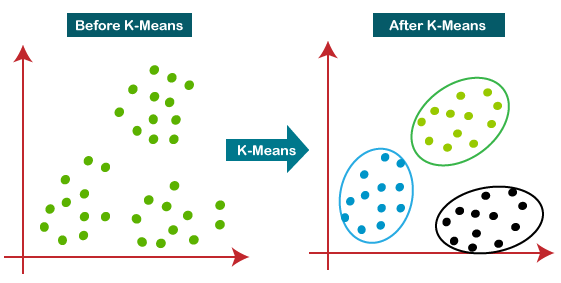
\includegraphics[width=0.75\textwidth]{2/figures/kmeans.png}
			\caption[El algoritmo de K medias]{El algoritmo de K medias.\\
			Fuente: \cite{tec_sancho2018supnosup}. \citetitle{tec_sancho2018supnosup}.}
			\label{2:fig3}
		\end{center}
	\end{figure}
		
	Debido a su complejidad y dificultad de implementación, este tipo de aprendizaje automático no se utiliza tan frecuentemente como el aprendizaje supervisado, a pesar de que abre las puertas a la resolución de problemas que los humanos normalmente no abordarían, según \parencite{tec_sancho2018supnosup}

	\item \textbf{Aprendizaje semisupervisado}: Hasta el momento, todos los datos enviados han sido etiquetados con el resultado deseado o no han sido etiquetados en absoluto. El aprendizaje automático semisupervisado utiliza ambos. El costo de etiquetar es bastante alto en muchas situaciones prácticas y, en el caso de grandes conjuntos de datos, se vuelve aburrido y requiere mucho tiempo. Además, proporcionar demasiados datos etiquetados puede hacer que el modelo tenga sesgos humanos. A pesar de que los datos sin etiquetar son desconocidos para la red, ofrecen información útil sobre los parámetros del grupo objetivo. que conduce a la conclusión de que se puede mejorar la precisión del modelo al incluir datos sin etiquetar y, al mismo tiempo, ahorrar tiempo y dinero en su construcción. Por ejemplo, la clasificación de páginas web, el reconocimiento de voz o la secuenciación genética pueden usar aprendizaje automático semisupervisado. En esos casos, los científicos de datos pueden acceder a grandes cantidades de datos sin etiquetarlos, y la tarea de etiquetarlos todos llevaría mucho tiempo, según \parencite{bk_zambrano2018supnosup}.

	Se puede comparar estos tres tipos de aprendizaje automático para el mismo uso, como clasificación, utilizando los datos recopilados hasta ahora:

	\begin{itemize}
		\item \textbf{Clasificación supervisada}: el algoritmo clasificará los tipos de páginas web según las etiquetas proporcionadas desde el principio, según \parencite{bk_zambrano2018supnosup}.
		\item \textbf{Agrupación no supervisada}: el algoritmo buscará patrones y características que ayudan a agrupar páginas web en grupos, según \parencite{bk_zambrano2018supnosup}.
		\item \textbf{Clasificación semi no supervisada}: identificará varios grupos de páginas web utilizando los datos etiquetados, luego utilizará los datos no etiquetados para establecer los límites de esos grupos de páginas web y buscar otros tipos que posiblemente no aparezcan en los datos etiquetados, según \parencite{bk_zambrano2018supnosup}.
	\end{itemize}
	

	\item \textbf{Aprendizaje por refuerzo}: junto con el aprendizaje supervisado y no supervisado, es el aprendizaje por refuerzo. Como se muestra en la Figura 17, se compone de cinco componentes principales: el agente, el entorno, el estado, la acción y la recompensa. Utilizando su interacción con el entorno, RL busca maximizar la recompensa y reducir el riesgo. El algoritmo RL (también conocido como agente) mejorará el entorno a intervalos regulares experimentando varios estados potenciales. Los agentes seleccionarán automáticamente el comportamiento ideal para maximizar el rendimiento. La retroalimentación, también conocida como recompensa, es lo que permite al agente mejorar su comportamiento, según \parencite{bk_sutton2018rl}.
	
	\begin{figure}[h]
		\begin{center}
			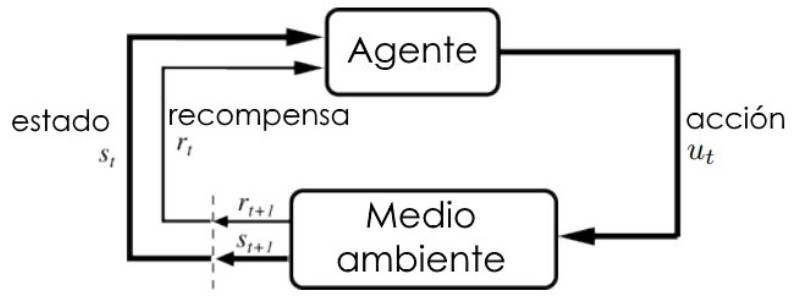
\includegraphics[width=0.60\textwidth]{2/figures/aprendizaje_refuerzo.jpg}
			\caption[Características del Aprendizaje por Refuerzo]{Características del Aprendizaje por Refuerzo.\\
				Fuente: \cite{bk_sutton2018rl}. \textit{Finite Markov Decision Processes}. (p. 48)}
			\label{2:fig4}
		\end{center}
	\end{figure}
	
\end{itemize}

\subsection{Aprendizaje Profundo}

Desde que llegó la Inteligencia Artificial hace un tiempo, tiene una amplia gama de aplicaciones y se divide en muchas ramas, como se menciona en \parencite{gl_sas_deeplearning}. El aprendizaje profundo es un subconjunto del aprendizaje automático, que es en sí mismo un subcampo de la IA. La Figura 18 es una representación visual de la relación entre AI, ML y DL.

\begin{figure}[!ht]
	\begin{center}
		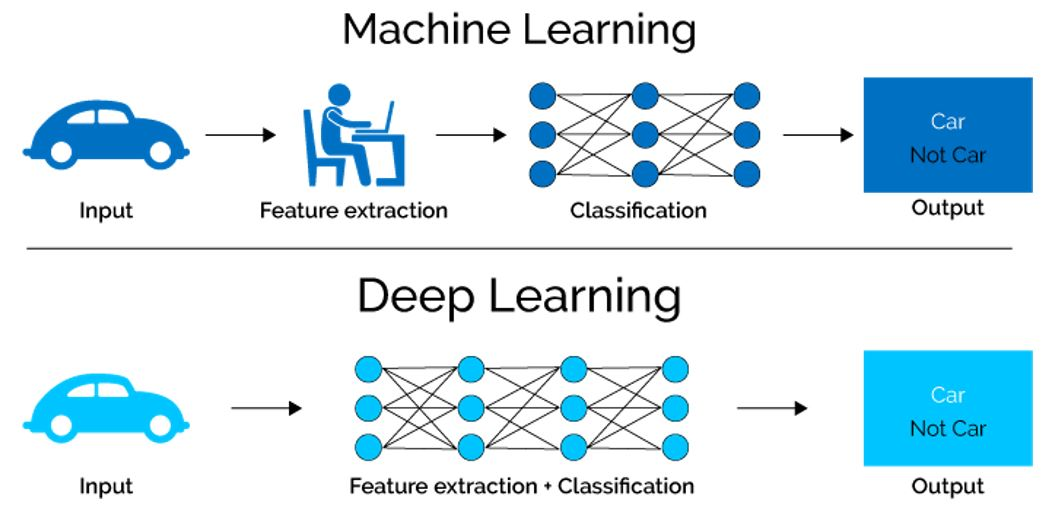
\includegraphics[width=0.50\textwidth]{2/figures/deeplearning_machinelearning.jpg}
		\caption[Relación entre IA, ML y DL]{Relación entre IA, ML y DL.\\
		Fuente: \cite{tec_cook2018deeplearning}. \textit{Most Popular 20 Free Online Courses to Learn Deep Learning}.}
		\label{2:fig5}
	\end{center}
\end{figure}

El aprendizaje profundo no solo permite representar datos de la manera correcta, sino que también permite que la computadora aprenda programas informáticos de varios pasos al incluir el concepto de profundidad en sus modelos. Como se muestra en la Figura 19, cada capa de representación puede interpretarse como el estado de la memoria de la computadora. Las computadoras interpretan las imágenes como una colección de valores de píxeles que representan escenas de nuestra realidad. Según \parencite{tec_cook2018deeplearning}, identificar un objeto o mapear su identidad a partir de esos valores es una tarea difícil para las máquinas y puede resultar casi imposible cuando se intenta aprender este mapeo directamente.

\begin{figure}[!ht]
	\begin{center}
		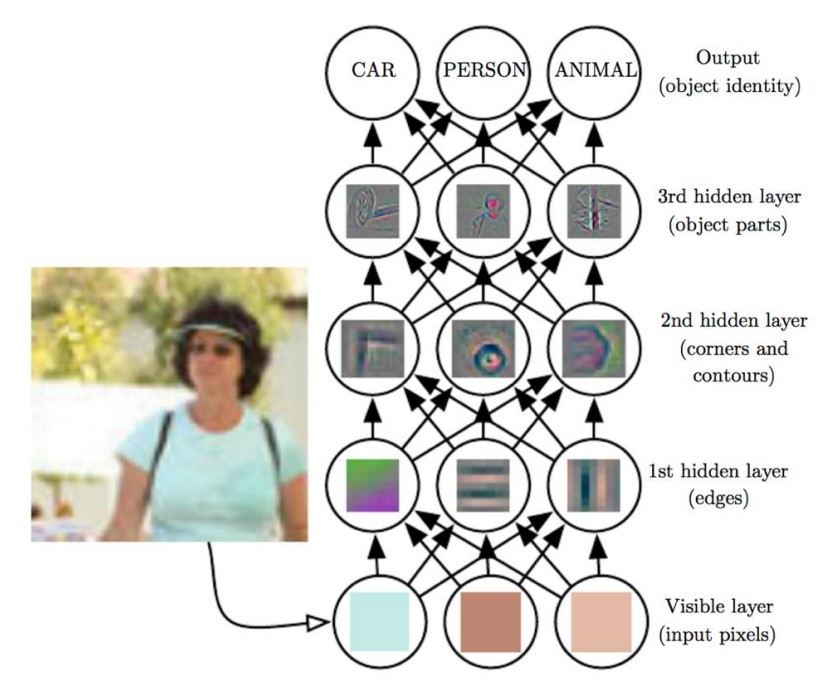
\includegraphics[width=0.70\textwidth]{2/figures/deeplearning_machinelearning2.jpg}
		\caption[Modelo de aprendizaje profundo]{Modelo de aprendizaje profundo.\\
		Fuente: \cite{tec_cook2018deeplearning}. \textit{Most Popular 20 Free Online Courses to Learn Deep Learning}.}
		\label{2:fig6}
	\end{center}
\end{figure}


\subsection{Aprendizaje Profundo Multimodal}
Como se muestra en la Figura 19, el fundamento del aprendizaje profundo multimodal es la integración de diversas modalidades a través del uso de redes neuronales profundas. \parencite{bk_deng2018deeplearningnlp}.

\begin{figure}[!ht]
	\begin{center}
		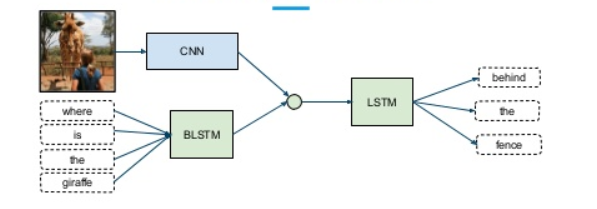
\includegraphics[width=0.85\textwidth]{2/figures/multimodal_network.png}
		\caption[Modelo que combina imágenes y texto]{Modelo que combina imágenes y texto.\\
		Fuente: \cite{tec_nishida2015multimodal}. \textit{Multimodal gesture recognition using multi-stream recurrent neural network}.}
		\label{2:fig7}
	\end{center}
\end{figure}

Las señales de diferentes modalidades aportan información complementaria sobre diversos aspectos de un objeto, evento o actividad, lo que permite a los modelos multimodales hacer inferencias más robustas. Entre las técnicas multimodales existentes se encuentran la fusión temprana y tardía, la integración de modelos, el ensamblado de modelos y las redes neuronales profundas. Cuando estas características se combinan para tomar decisiones, se utilizan enfoques aditivos, los cuales recopilan información útil y mejoran la precisión de las predicciones de manera colectiva. \parencite{bk_deng2018deeplearningnlp}

\cite{tec_baheti2020introduction_mdl} afirman que el uso de modelos multimodales mejora el rendimiento de las redes neuronales y permite una extracción más efectiva de características, lo que favorece predicciones mayores. Uno de las ventajas es que los datos de diferentes fuentes ofrecen información complementaria que revela patrones ocultos que no se pueden ver cuando las modalidades se analizan individualmente, mejorando así la precisión de las predicciones.

Según \cite{tec_brownlee2018stacked_models}, se puede mejorar la calidad del promedio del modelo al considerar de manera ponderada las contribuciones de cada submodelo a la predicción combinada. Este enfoque se conoce como "generalización apilada" y se divide en dos niveles.

\begin{itemize}
    \item Nivel 0: Este nivel utiliza los datos de entrada del conjunto de entrenamiento para enseñar a los modelos a hacer predicciones.
    \item Nivel 1: Aquí, los datos provienen de las salidas de los modelos del nivel anterior, que se utilizan como entradas para enseñar a los modelos de este nivel, también conocidos como meta-aprendices o generalizadores.
\end{itemize}

Dentro de los modelos ensamblados apilados, se emplean dos enfoques distintos:

\begin{itemize}
    \item Modelo apilado separado: Consiste en generar un conjunto de datos de entrada a partir de las predicciones combinadas de otros modelos, los cuales se utilizan para entrenar un nuevo modelo y realizar la predicción final.
    \item Modelo apilado integrado: Este enfoque permite el uso de redes neuronales y un modelo multicéfalo compuesto por otros modelos preentrenados. Estos modelos no necesitan mantener la misma estructura, ya que sus capas se designan como "no entrenables" para evitar la actualización de sus pesos antes de generar predicciones. Los resultados de los submodelos se incorporan directamente en el generalizador.
\end{itemize}

\begin{figure}[!ht]
	\begin{center}
		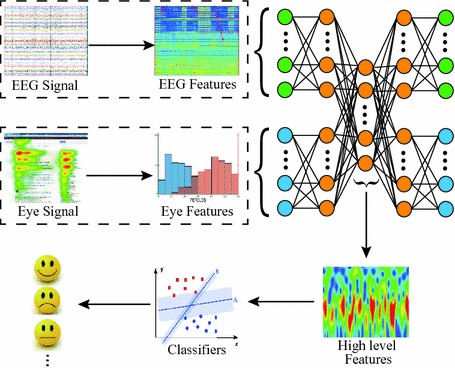
\includegraphics[width=0.79\textwidth]{2/figures/multimodal_deep_learning_example.jpg}
		\caption[Un modelo multimodal para las señales de la vista]{Un modelo multimodal para las señales de la vista.\\
		Fuente: \cite{tec_baheti2020introduction_mdl}. \citetitle{tec_baheti2020introduction_mdl}.}
		\label{2:fig7}
	\end{center}
\end{figure}

\subsection{Inteligencia Artificial Generativa}

La inteligencia artificial generativa es el campo de la ciencia que estudia cómo crear inteligencia totalmente automatizada. Esto contrasta con el campo de la inteligencia artificial moderna, que investiga cómo los humanos comprenden y construyen la inteligencia. La construcción manual es lo que hacen los investigadores, pero la parte "por humanos" de la definición de IA suele ser una variable oculta en la construcción de los sistemas de IA contemporáneos. Aunque la diferencia puede parecer sutil, incluso innecesaria, la construcción automatizada requiere una perspectiva completamente nueva, que no está disponible en la literatura sobre IA actual. No importa si los humanos comprenden cómo funcionan los mecanismos internos de una máquina en la Inteligencia Artificial Generativa, aunque podría ayudar a los investigadores en su búsqueda de la creación de máquinas inteligentes. Lo que importa es que la máquina pueda controlar y dirigir el proceso de creación de estructuras internas en la dirección deseada. Es como criar hijos: los seres humanos no son conscientes de los procesos mentales, pero interactúan con sus hijos en un nivel diferente al hablar de sus sustratos neuronales. En lugar de eso, utilizan una variedad de máquinas clasificadoras para diferenciar los comportamientos positivos de los negativos, que podrían ser beneficiosos para el niño cuando sea mayor. Los castigos corporales, los institutos educativos, los medios de comunicación y otros lugares son algunos de los usos de estas máquinas clasificadoras, según \parencite{th_zant2010genai}

A continuación, ofrecemos una variedad de categorías de modelos de inteligencia artificial generativa.

\begin{itemize}
	\item \textbf{Modelos de difusión}: crean nuevos datos iterando cambios aleatorios controlados en una muestra de datos previa. Empezan con los datos originales y luego agregan cambios sutiles, también conocidos como ruido, que hacen que gradualmente pierdan la similitud con el original. Este ruido se controla minuciosamente para garantizar que los datos generados sigan siendo consistentes y realistas. El modelo de difusión invierte el proceso después de agregar ruido en varias iteraciones. Como se muestra en la Figura 22, la eliminación de ruido inversa crea una muestra de datos nueva que se asemeja a la original, según \parencite{tec_amaz2023iagen}.
	
	\begin{figure}[!ht]
		\begin{center}
			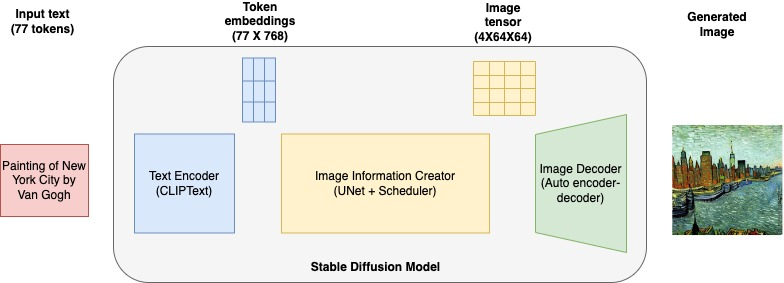
\includegraphics[width=0.85\textwidth]{2/figures/modelosdedifusion.jpg}
			\caption[Modelos de difusión]{Modelos de difusión.\\
			Fuente: \cite{tec_amaz2023iagen}. \citetitle{tec_amaz2023iagen}.}
			\label{2:fig8}
		\end{center}
	\end{figure}

	\item \textbf{Redes generativas adversativas}: compiten con dos redes neuronales. La primera red, también conocida como generador, agrega ruido aleatorio para crear muestras de datos falsas. La segunda red, conocida como discriminador, ayuda a distinguir entre los datos reales y falsos generados por el generador. El generador mejora continuamente su capacidad de generar datos realistas, mientras que el discriminador mejora su capacidad de distinguir entre lo real y lo falso. Hasta que el generador produzca datos tan persuasivos que el discriminador no pueda diferenciarlos de los datos reales, este proceso adversativo termina, según \parencite{tec_amaz2023iagen}.

	\item \textbf{Autocodificadores variacionales}: aprenden sobre el espacio latente, una pequeña representación de datos. La representación matemática de los datos se conoce como espacio latente. Puede verse como un código único que representa los datos en función de cada característica. Por ejemplo, cuando se estudian los rostros, el espacio latente contiene números que representan la forma de las orejas, los pómulos, la nariz y los ojos. Las dos redes neuronales utilizadas por los VAE son el codificador y el decodificador. Para cada dimensión del espacio latente, la red neuronal del codificador mapea los datos de entrada a una media y una varianza. crea una muestra aleatoria utilizando la distribución normal gaussiana. Este ejemplo es un punto en el espacio latente, y como se puede ver en la Figura 23, representa una versión comprimida y simplificada de los datos de entrada, según \parencite{tec_amaz2023iagen}.
	
	\begin{figure}[!ht]
		\begin{center}
			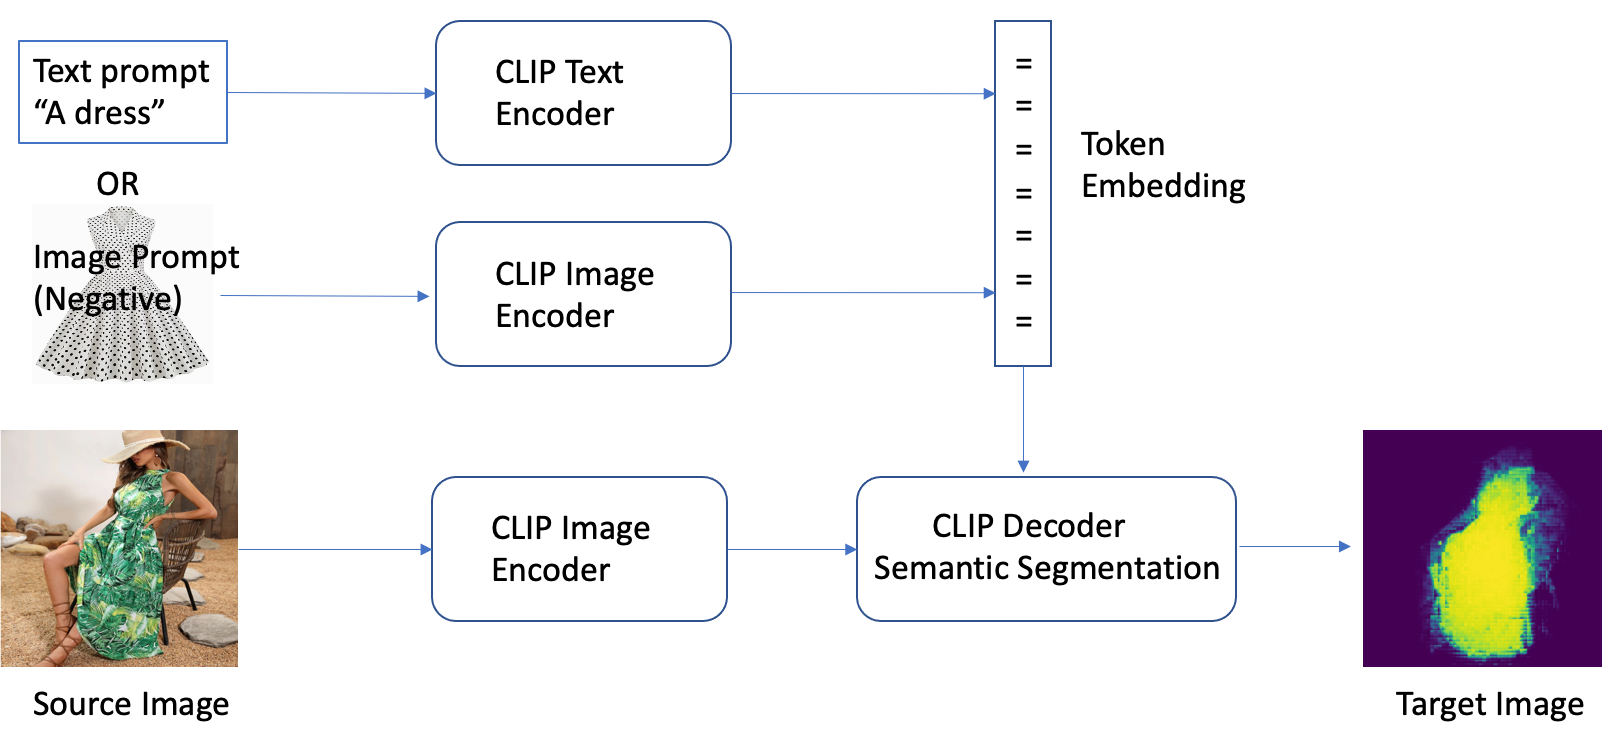
\includegraphics[width=0.85\textwidth]{2/figures/autocodificadoresvariacionales.png}
			\caption[Autocodificadores variacionales]{Autocodificadores variacionales.\\
			Fuente: \cite{tec_amaz2023iagen}. \citetitle{tec_amaz2023iagen}.}
			\label{2:fig9}
		\end{center}
	\end{figure}
\end{itemize}


\subsection{Modelos de Predicción y Análisis de Datos Espaciales}

Los modelos estadísticos se utilizan para prever comportamientos futuros mediante la recopilación de datos actuales e históricos, la creación de modelos estadísticos, la realización de predicciones y la validación continua a medida que se recopilan más datos. Estos modelos predictivos identifican patrones ocultos y usan los sucesos anteriores con el fin de calcular las diversas opciones de si el individuo presente algún cambio tiempo después. \parencite{gl_gartner2019pm}

El análisis espacial es una colección de técnicas y modelos que utilizan explícitamente referencias espaciales para cada valor de datos u objeto especificado en el sistema en estudio. Los métodos de análisis espacial necesitan hacer suposiciones o basarse en datos para describir las relaciones espaciales o interacciones espaciales entre casos. Los resultados de cualquier análisis espacial no son iguales cuando se reordenan la distribución espacial de valores o se reconfigura la estructura espacial del sistema. \parencite{bk_haining2003spdat}

Al realizar un análisis estadístico, es necesario tener en cuenta muchas características de los datos espaciales. El análisis de la dependencia espacial es crucial para el análisis de datos espaciales y central, por ejemplo, para realizar predicciones espaciales o especificar diseños de muestreo. Sin embargo, concentrarse demasiado en este aspecto de los datos espaciales puede llevar al analista a ignorar otras cuestiones. Por ejemplo, el impacto de una partición de área en la precisión de un estimador o el conjunto más amplio de supuestos y efectos de los datos que determinan si un modelo puede considerarse apropiado para el propósito previsto. Por lo tanto, el análisis de datos espaciales es una rama del análisis de datos más amplio. \parencite{bk_haining2003spdat}

Existe, por lo tanto, un papel importante para las áreas de la teoría estadística desarrolladas para manejar otros tipos de datos no espaciales, al definir las habilidades y conceptos necesarios para realizar un análisis adecuado de datos espaciales. Se mantiene un vínculo con el cuerpo más amplio de teoría y métodos estadísticos al adoptar esta definición bastante más amplia de análisis de datos espaciales. \parencite{bk_haining2003spdat}

Los métodos utilizados para el análisis espacial son:

\begin{itemize}
	\item \textbf{Análisis Exploratorio de Datos Espaciales (ESDA)}:describe cómo utilizar técnicas de visualización y análisis numérico para explorar y comprender la estructura espacial de los datos como se ve en la Figura 24. Esto incluye métodos numéricos para identificar propiedades de los datos espaciales, como suavización espacial, métodos de agrupación y comparación de mapas, así como métodos visuales para explorar los datos espaciales, como mapas y gráficos. \parencite{bk_haining2003spdat}
	
	\begin{figure}[h]
		\begin{center}
			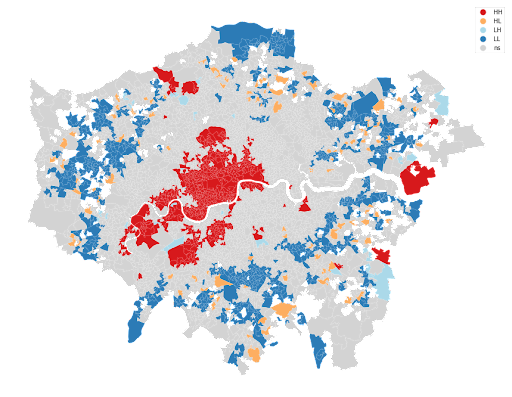
\includegraphics[width=0.65\textwidth]{2/figures/esda.png}
			\caption[Análisis Exploratorio de Datos Espaciales (ESDA)]{Análisis Exploratorio de Datos Espaciales (ESDA).\\
			Fuente: \cite{bk_haining2003spdat}. \citetitle{bk_haining2003spdat}. (p. 181)}
			\label{2:fig10}
		\end{center}
	\end{figure}
		

	\item \textbf{Modelos de Análisis Espacial}:para estimar y modelar el semivariograma, se presentan modelos de análisis espacial, como kriging con datos gaussianos que se muestra en la Figura 25. Esto es particularmente útil para datos de superficies continuos. \parencite{bk_haining2003spdat}
	
	\begin{figure}[h]
		\begin{center}
			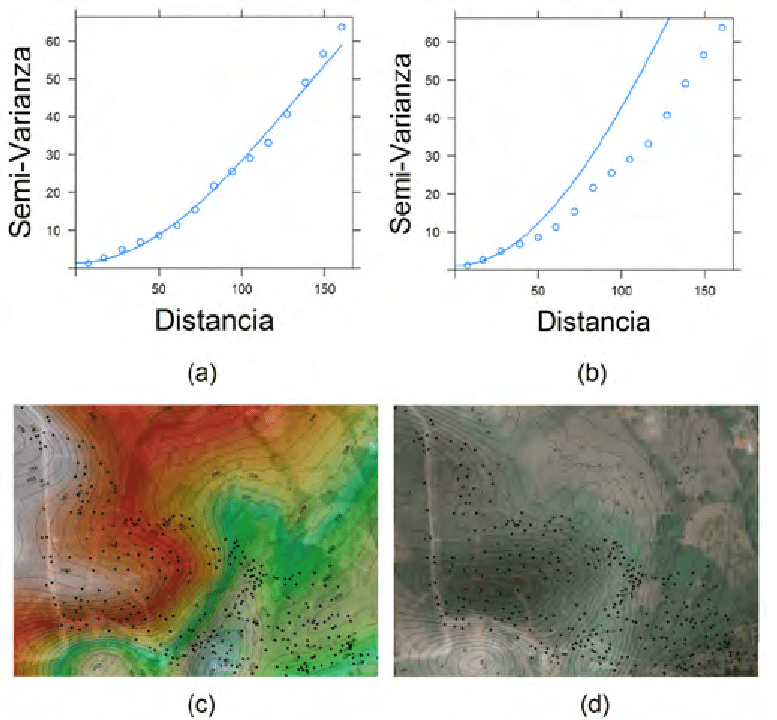
\includegraphics[width=0.70\textwidth]{2/figures/kriging.jpg}
			\caption[El modelo gaussiano isotrópico; el modelo gaussiano anisotrópico ajustado; la predicción de Kriging Simple Residual; y la varianza de Kriging Simple Residual.]{El modelo gaussiano isotrópico; el modelo gaussiano anisotrópico ajustado; la predicción de Kriging Simple Residual; y la varianza de Kriging Simple Residual.\\
			Fuente: \cite{bk_haining2003spdat}. \citetitle{bk_haining2003spdat}. (p. 352)}
			\label{2:fig11}
		\end{center}
	\end{figure}

	\item \textbf{Logistic Regression}: modela fenómenos espaciales como las relaciones entre variables espaciales y no espaciales. \parencite{bk_haining2003spdat}
	
	\begin{figure}[h]
		\begin{center}
			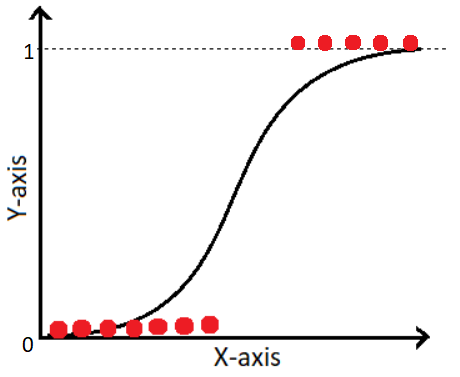
\includegraphics[width=0.70\textwidth]{2/figures/logisticregression.png}
			\caption[Regresión Logística]{Regresión Logística.\\
			Fuente: \cite{bk_haining2003spdat}. \citetitle{bk_haining2003spdat}. (p. 358)}
			\label{2:fig12}
		\end{center}
	\end{figure}
\end{itemize}
	
\subsection{Redes Neuronales Recurrentes y Redes Neuronales Convolucionales}

Las Redes Neuronales Convolucionales (CNN) y las Redes Neuronales Recurrentes (RNN) son algunas de las técnicas de aprendizaje profundo que se utilizan actualmente para resolver problemas de lenguaje natural. A continuación se describen algunos de los más comunes, junto con las principales características y diferencias de los ejemplos ya mencionados.

\begin{itemize}
	\item \textbf{Redes Neuronales Convolucionales}: Hoy en día, el procesamiento de imágenes, que incluye problemas de clasificación y visión por computadora, es una de sus aplicaciones más relevantes. El proyecto de Yann LeCun, ImageNet, utiliza el reconocimiento de objetos en imágenes.
	
	Estas redes también se utilizan para clasificar textos. Ronan Collobert y Jason Weston modificaron la arquitectura y los parámetros internos de las CNN para usarlas en tareas de procesamiento de lenguaje natural. La Figura \ref{2:fig40} muestra la estructura de una CNN para problemas de procesamiento de información natural. \parencite{bk_kamath2019deeplearning_nlp_sr}
	\begin{figure}[!ht]
		\begin{center}
			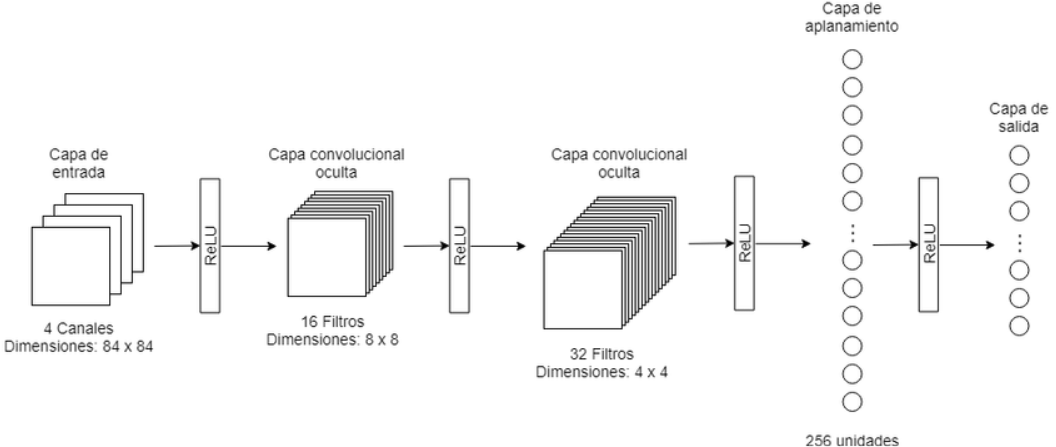
\includegraphics[width=0.95\textwidth]{2/figures/cnn_nlp.png}
			\caption[Arquitectura de un modelo CNN]{Arquitectura de un modelo CNN.\\
			Fuente: \cite{tec_kim2014convolutional}. \citetitle{tec_kim2014convolutional}. (p. 1747)}
			\label{2:fig40}
		\end{center}
	\end{figure}
	
	Debido a que se mueven a través de matrices en dos dimensiones, las convoluciones de imágenes suelen ser bidimensionales (2D). Sin embargo, debido a que están conformadas por vectores, las convoluciones unidimensionales son extremadamente útiles para las series de tiempo. La Figura \ref{2:fig41} compara los tipos de convolución en función del tamaño de la dimensión. \parencite{bk_rao2019nlp_pytorch}

 	El proceso de arquitectura CNN generalmente está situado en los problemas de clasificación de texto considerados en esta investigación y algunas priorizaciones relacionadas con el contenido del texto.

 	La ID genérica es la creación de los vectores de los códigos Mots para la matriz de entidad genérica, que es la misma que los unidimensionales para los mapas de características genéricos de la siguiente entrada. Para generar vectores nuevos y consistentes después de cada resultado, se reagrupan según la función de los criterios utilizados (por ejemplo, máximo, mínimo, mes, etc.) y luego se vinculan al valor.

	\item \textbf{Redes Neuronales Recurrentes}: son muy utilizadas porque los datos son secuencias. En la comunicación del ser humano, se sabe que los fonemas son secuencias de palabras, se puede usar un elemento dependiente para predecir la palabra que sigue de una oración. En la siguiente figura se puede ejemplificar una RNN. \parencite{bk_rao2019nlp_pytorch}
	\begin{figure}[!ht]
		\begin{center}
			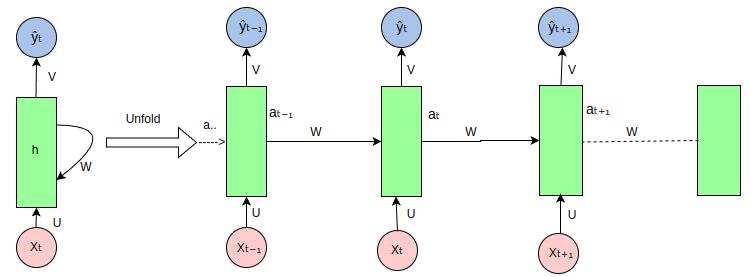
\includegraphics[width=0.95\textwidth]{2/figures/rnn.png}
			\caption[Modelo RNN]{Modelo RNN.\\
			Fuente: \cite{bk_rao2019nlp_pytorch}. \citetitle{bk_rao2019nlp_pytorch}. (p. 1747)}
			\label{2:fig41}
		\end{center}
	\end{figure}

	Para representar un estado determinado en una RNN se debe usar la siguiente fórmula:

	\begin{equation}\label{eq:RNN}
		s_i = \text{RSRNN}(x_i, s_{i-1}) = g(W[s_{i-1}; x_i] + b)
	\end{equation}
	\myequations{Fórmula para hallar el estado de una RNN}

	\item \textbf{Modelo Secuencia a Secuencia}: una técnica común en la traducción es la generación de lenguaje natural (NLG), basado en dos capas LSTM. De esto, 1° capa transforma la oración inicial para un "vector de pensamiento", mientras que en 2° capa decodifica la respuesta, como se se observa la Figura \ref{2:fig46}. \parencite{bk_deng2018deeplearningnlp}.
	
	\begin{figure}[!ht]
		\begin{center}
			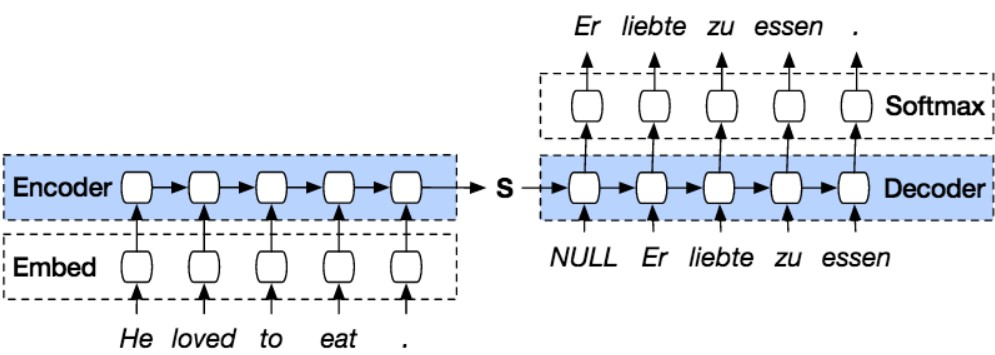
\includegraphics[width=0.67\textwidth]{2/figures/encoder-decoder.jpg}
			\caption[Modelo Seq2seq]{Modelo Seq2seq.\\
			Fuente: \cite{tec_kostadinov2019seq2seq}. \citetitle{tec_kostadinov2019seq2seq}.}
			\label{2:fig46}
		\end{center}
	\end{figure}	
\end{itemize}

Debido a que estos modelos no pueden incluir el texto en su estado original sin limpiarlo previamente, estos modelos requieren un preprocesamiento del contenido textual. La biblioteca Natural Language Toolkit (NLTK) de Python facilita la modelización y el trabajo con texto. Sus funciones incluyen dividir el texto en oraciones, tokenizar, eliminar puntos y palabras de parada, reducir palabras a su forma raíz y convertir palabras a su forma base o diccionario. \parencite{bk_brownlee2017deeplearning_nlp}

\subsection{Redes Generativas Antagónicas}

Las redes generadoras y discriminadoras son las dos redes que compiten entre sí en las Generative Adversarial Networks (GAN). El discriminador determina si los datos son reales o generados por el generador, mientras que la función del generador es producir nuevos datos que se asemejen al conjunto de datos de entrenamiento. \parencite{tec_goodfellow2014gan}

En este juego de suma cero, quien gana pierde. El generador tiene un alto error si el discriminador clasifica correctamente los datos generados, y viceversa. Debido a que dos tipos de redes trabajan juntos, el proceso de entrenamiento es esencial. \parencite{tec_goodfellow2014gan}

Las GAN se utilizan principalmente para producir datos que se asemejan a los de entrada. Esto puede ser simplemente para generar nuevos datos o para aumentar el tamaño de un conjunto de datos existente para entrenar otra red neuronal. \parencite{tec_goodfellow2014gan}

\subsubsection{Arquitectura de las GAN}

La Figura 30 muestra la relación entre el generador y el discriminador en una GAN. El discriminador debe determinar la procedencia de cada imagen que recibe, que puede provenir de un generador o de un conjunto de datos. Mientras tanto, los valores aleatorios se convierten en imágenes que el discriminador reconoce como pertenecientes al conjunto de datos a través del generador. \parencite{tec_goodfellow2014gan}

\begin{figure}[!ht]
	\begin{center}
		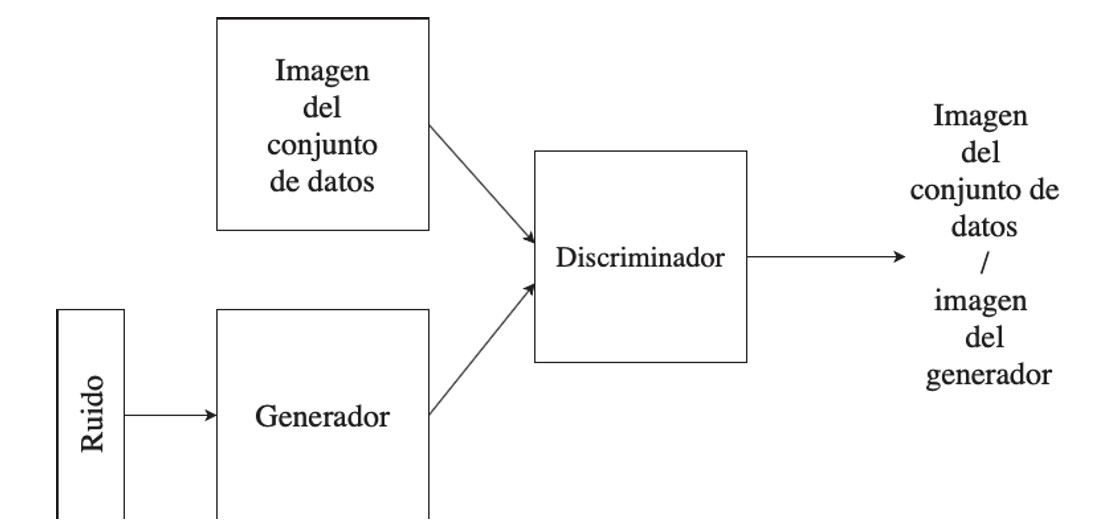
\includegraphics[width=0.75\textwidth]{2/figures/redgan.jpg}
		\caption[Red Generativa Antagónica de Imágenes]{Red Generativa Antagónica de Imágenes.\\
		Fuente: \cite{tec_goodfellow2014gan}. \citetitle{tec_goodfellow2014gan}.}
		\label{2:fig47}
	\end{center}
\end{figure}

El uso de GANs es amplia y no se limita a un tipo de datos específico. La Figura 31 muestra una GAN con un generador y un discriminador de dos capas. En el generador, cada capa es gradualmente más grande, mientras que en el discriminador, cada capa se vuelve más pequeña hasta que se encuentra una neurona en la última capa. \parencite{tec_goodfellow2014gan}

\begin{figure}[!ht]
	\begin{center}
		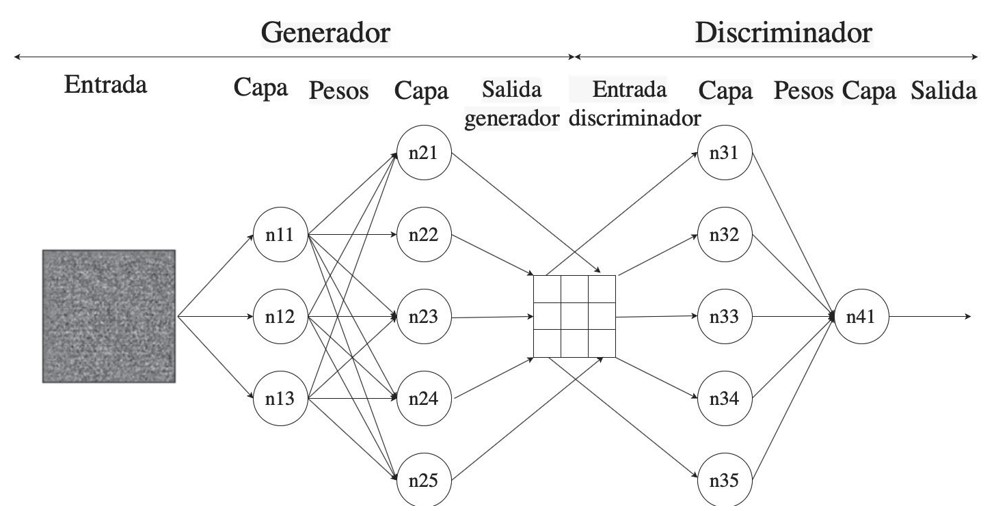
\includegraphics[width=0.75\textwidth]{2/figures/redgan2.jpg}
		\caption[Red Generativa Antagónica de Imágenes]{Red Generativa Antagónica de Imágenes.\\
		Fuente: \cite{tec_goodfellow2014gan}. \citetitle{tec_goodfellow2014gan}.}
		\label{2:fig48}
	\end{center}
\end{figure}

Como se muestra en la Figura 32 con imágenes en blanco y negro, la entrada del generador es una distribución aleatoria gaussiana. Su salida es comparable a la del conjunto de datos, y la capa de salida debe tener suficientes neuronas dispuestas de manera adecuada para producir datos con la misma estructura que el conjunto de datos original, ya sea imágenes, audio o cualquier otro tipo de datos. Por ejemplo, si se quieren imágenes de 20 x 20 píxeles, el generador debe producir 400 neuronas. Cada capa del generador es más grande que la anterior y generalmente utiliza la activación Selu, excepto la capa final, que utiliza Sigmoide. \parencite{tec_goodfellow2014gan}

\begin{figure}[!ht]
	\begin{center}
		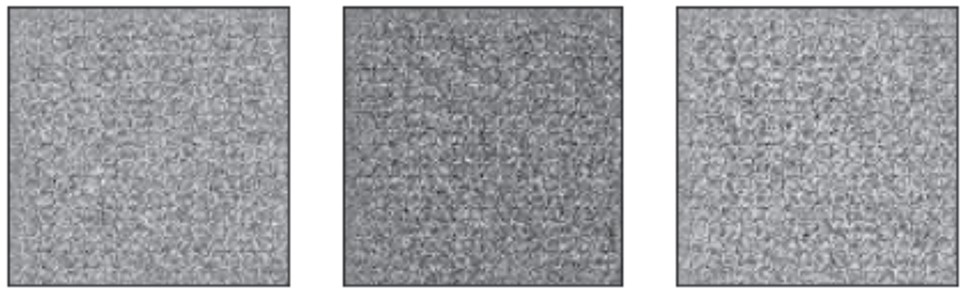
\includegraphics[width=0.75\textwidth]{2/figures/redgan3.jpg}
		\caption[Imágenes de Ruido Gaussiano]{Imágenes de Ruido Gaussiano.\\
		Fuente: \cite{tec_goodfellow2014gan}. \citetitle{tec_goodfellow2014gan}.}
		\label{2:fig49}
	\end{center}
\end{figure}

Los datos del conjunto de datos o los creados por el generador son la entrada del discriminador. Su salida consiste en una neurona con un solo valor numérico que intenta determinar si la entrada proviene del generador o del conjunto de datos. Por lo general, cada capa del discriminador contiene menos neuronas hasta que solo queda una neurona en la capa más alta. \parencite{tec_goodfellow2014gan}

\subsubsection{Entrenamiento de las GAN}

En el primer paso del proceso, el discriminador recibe capacitación para diferenciar entre imágenes reales y imágenes creadas por el generador. El generador se entrena para crear imágenes en el segundo paso, pero los pesos del discriminador no se actualizan en este caso. Las imágenes generadas se etiquetan como reales y el generador ajusta sus pesos para que el discriminador piense que son reales. Esto mejora su capacidad para generar imágenes más parecidas al conjunto de datos original mediante la retropropagación del gradiente. \parencite{bk_geron2019machilear}

Hasta que el generador produzca resultados satisfactorios, estos pasos se repiten. El discriminador se entrena con las imágenes recién generadas y luego se enseña al generador con lo que el discriminador ha aprendido. \parencite{bk_geron2019machilear}

\subsubsection{Dificultades del entrenamiento de las GAN}

El juego de suma cero en las GAN significa que cuanto menor sea el error de uno de los elementos, mayor será el error del otro. Cuando ninguna de las dos redes cambia su estrategia, se alcanza un estado de equilibrio de Nash. Este equilibrio se alcanza cuando el generador crea imágenes perfectamente realistas y el discriminador intenta clasificarlas con una probabilidad del 50\% como generadas o del conjunto de datos. Es necesario aplicar la técnica de prueba y error durante el entrenamiento de una GAN porque no se puede garantizar que se llegue a este equilibrio. \parencite{bk_geron2019machilear}

Cuando el conjunto de datos incluye varias clases, como diferentes tipos de mascotas (gatos, perros y conejos), el entrenamiento de una GAN se vuelve más difícil. Aunque el objetivo del discriminador sigue siendo distinguir entre imágenes reales y generadas, puede haber una clase en la que el generador produzca más imágenes que el discriminador clasifique como reales, mientras que en otras clases puede haber deficiencias. Por ejemplo, el generador puede ser muy hábil en la creación de imágenes de perros, pero no lo es en otras categorías. Esto puede llevar al generador a producir más imágenes de perros y olvidarse de cómo producir imágenes de otras clases. Al recibir principalmente imágenes de perros, el discriminador puede fallar en clasificar correctamente las imágenes de otras clases. \parencite{bk_geron2019machilear}

\subsection{Generación de Imágenes}

En los últimos años, ha habido una notable evolución en la generación de imágenes a través de la inteligencia artificial, impulsada por dos modelos generativos importantes: los autocodificadores variacionales y las redes generativas antagónicas, particularmente las que utilizan capas convolucionales. Aunque existen otras técnicas para generar imágenes no relacionadas con la IA, como las utilizadas en cine o videojuegos, se utiliza el término "imágenes generadas por ordenador" o CGI en inglés para estos fines. A pesar de que este término incluye una variedad de técnicas, en su mayoría implica modelar objetos en tres dimensiones, aplicar texturas y renderizarlos en dos dimensiones. \parencite{tec_kingma2019variat}

DCGAN, o GAN con capas convolucionales, es una herramienta común para la generación de imágenes. Como las GAN convencionales, tiene un generador y un discriminador. La Figura 33 muestra la estructura típica de una DCGAN, que utiliza una capa inicial de tres neuronas, seguida de tres capas de normalización y convolución transpuesta, produciendo una imagen a color. El discriminador, por otro lado, utiliza dos capas de convolución, dos capas de reducción y dos capas totalmente conectadas. \parencite{tec_kingma2019variat}

\begin{figure}[!ht]
	\begin{center}
		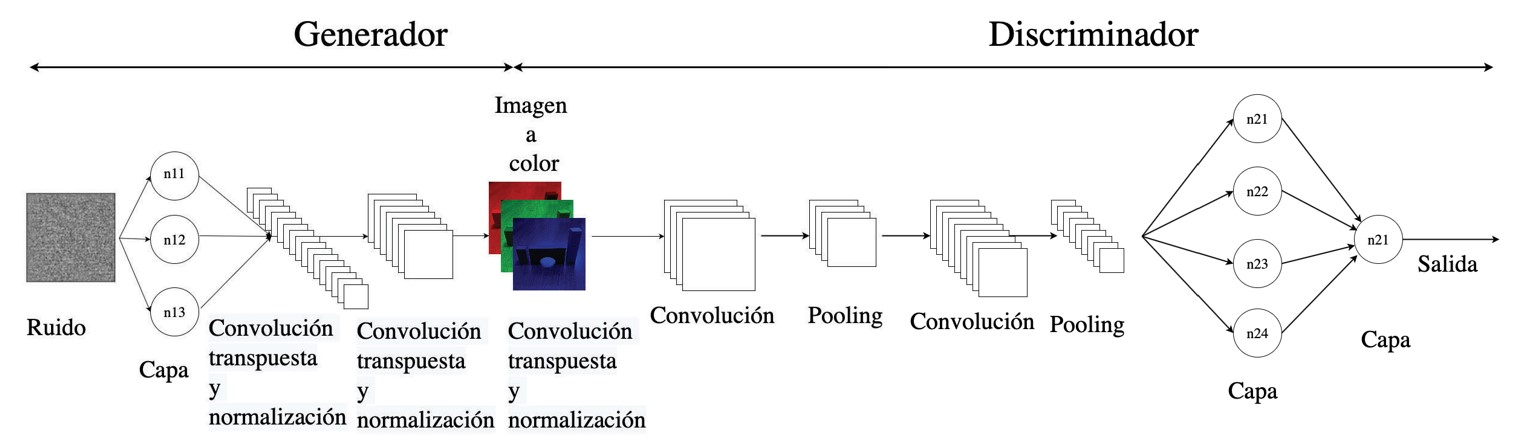
\includegraphics[width=1\textwidth]{2/figures/genimagenes.jpg}
		\caption[Arquitectura de Red Generativa Antagónica con Capas Convolucionales (DCGAN)]{Arquitectura de Red Generativa Antagónica con Capas Convolucionales (DCGAN).\\
		Fuente: \cite{tec_kingma2019variat}. \citetitle{tec_kingma2019variat}.}
		\label{2:fig50}
	\end{center}
\end{figure}

La entrada de ruido del generador se procesa a través de capas de normalización y convolución transpuesta para crear la imagen deseada. La entrada del discriminador conecta la salida del generador, que clasifica las imágenes como generadas o reales. El discriminador generalmente se compone de capas convolucionales y redes neuronales, con una sola neurona de salida con activación Sigmoide. \parencite{tec_kingma2019variat}

Los autocodificadores variacionales (VAE), que tienen similitudes con las GAN, son otra técnica común para generar imágenes. Los VAE consisten en un codificador y un decodificador y tienen como objetivo reconstruir las entradas de la red. El codificador reduce gradualmente la dimensionalidad de los datos hasta obtener una representación latente, que el decodificador reconstruye posteriormente. Los VAE pueden producir datos similares a los de entrenamiento y aplicar aleatoriedad para generar nuevas muestras. \parencite{tec_kingma2013bayes}

La interpolación de datos es otra aplicación de los autocodificadores y los VAE; en este caso, la representación latente de dos datos se combina ponderadamente para generar nuevas muestras. Interpolar entre dos muestras ya existentes permite la creación de nuevas instancias de datos. \parencite{tec_kingma2013bayes}

\newpage

\section{Marco Conceptual}
\subsection{Redes Inalámbricas}
Una red inalámbrica es un sistema de comunicación de datos flexible que reduce la necesidad de conexiones físicas al enviar y recibir datos por aire a través de medios inalámbricos, como la tecnología de radiofrecuencia. Las redes de datos están experimentando un cambio significativo gracias a la revolución de las comunicaciones inalámbricas. Los recientes avances en las redes y la tecnología inalámbrica han permitido que la gran mayoría de los dispositivos inalámbricos que se utilizan hoy en día se conecten fácilmente. Es necesario maximizar el uso de los recursos del espectro para permitir que millones de dispositivos inalámbricos se conecten inalámbricamente. \parencite{tec_pundalik2023anwirnet}

Las redes inalámbricas utilizan ondas electromagnéticas para transferir información entre lugares sin tener conexiones físicas. Las ondas de radio suelen denominarse portadoras de radio, ya que sólo envían energía a un receptor distante. Los datos que se transfieren se superponen a la onda de radio para garantizar una extracción precisa en el extremo receptor. Debido a que la frecuencia de la información de modulación o la velocidad de bits se suman a la portadora de radio después de que los datos se superponen (modulan) sobre ella, la señal de radio tiene muchas frecuencias. Si las ondas de radio se envían en diferentes frecuencias de radio, varias portadoras de radio pueden coexistir en el mismo espacio sin interferir entre sí. Las señales de radio, los formatos de datos y la arquitectura de la red son los tres componentes de una red inalámbrica. Dado que estos tres elementos no están relacionados entre sí, deben describirse al construir una nueva red. Mientras que la señal de radio opera en la capa física, el formato de datos tiene un impacto en varios niveles superiores del modelo de referencia OSI. Las estaciones base y los adaptadores de interfaz de red inalámbrica son componentes de la estructura de la red que envían y reciben señales de radio. Cada computadora y estación base en una red inalámbrica tiene adaptadores de interfaz de red que transforman los datos digitales en señales de radio, que luego se envían a otros dispositivos conectados. Además, reciben y transforman las señales de radio entrantes de otros componentes de la red en datos digitales. Los formatos de datos, las arquitecturas de red y las señales de radio son distintos para cada servicio de datos inalámbricos de banda ancha. \parencite{tec_rafaqat2019surveywir}

Las redes inalámbricas se clasifican normalmente en cinco grupos distintos. La región de aplicación y el rango de señal son los principales criterios utilizados para esta clasificación (Figura 30). Las redes inalámbricas en el primer grupo, WBAN, conectan dispositivos en la superficie del cuerpo entre sí. Las señales de estas redes pueden alcanzar un máximo de dos metros. El segundo grupo, conocido como WPAN, está compuesto por redes inalámbricas con un alcance de señal mínimo de 10 metros que se utilizan para conectar varios dispositivos entre sí. El tercer grupo cumple con el estándar de redes inalámbricas, que busca cubrir un edificio o habitación como máximo. El alcance de señal de este grupo, conocido como WLAN, suele ser de 30 metros en interiores y de 100 a 200 metros en exteriores. El término fidelidad inalámbrica (Wi-Fi o IEEE 802.11) se usa con frecuencia para describir la tecnología inalámbrica. La WMAN, la cuarta clase de red inalámbrica, permite a los usuarios conectarse a Internet con un alcance de señal de entre 5 y 20 kilómetros. Este protocolo a menudo se conoce como IEEE 802.16-2001, también conocido como interoperabilidad mundial para acceso por microondas (WiMAX). El WWAN es el grupo final. Las redes WWAN (redes basadas en GSM y CDMA) ofrecen conexiones inalámbricas en una área mucho más amplia que el grupo anteriormente mencionado utilizando la infraestructura de red de los operadores móviles. \parencite{tec_ieee2010draft}
\begin{figure}[!ht]
	\begin{center}
		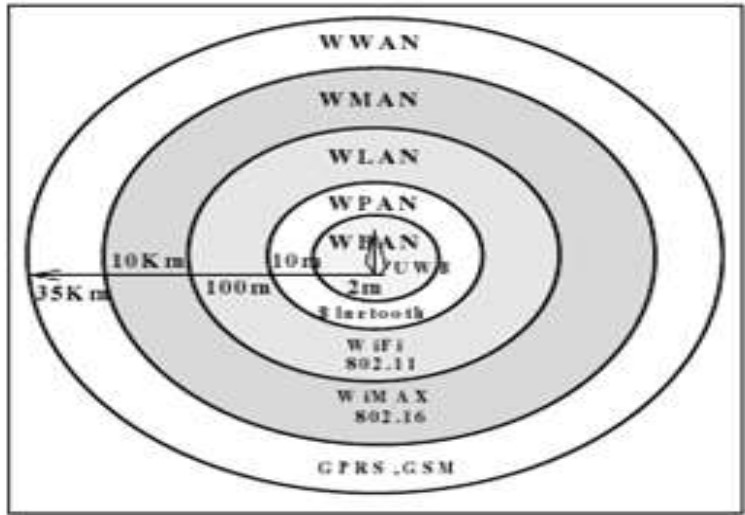
\includegraphics[width=0.5\textwidth]{2/figures/clasificacionredes.jpg}
		\caption[Clasificación de redes inalámbricas con su alcance de señal]{Clasificación de redes inalámbricas con su alcance de señal.\\
			Fuente: \cite{tec_ieee2010draft}. \citetitle{tec_ieee2010draft}.}
		\label{2:fig52}
	\end{center}
\end{figure}

\subsection{Calidad de Servicio (QoS)}
La expansión de las redes de datos de alta velocidad depende de la calidad de servicio (QoS). Esto es particularmente cierto cuando se trata de cumplir con las limitaciones de velocidad de datos y latencia de paquetes de los consumidores de datos en tiempo real. Al transferir un flujo de paquetes desde el origen al destino, la red debe cumplir con ciertos requisitos de calidad de servicio (QoS). Debido a este requisito, las redes que utilizan comunicación inalámbrica enfrentan desafíos especiales. La calidad de un canal inalámbrico varía significativamente entre los usuarios y cambia enormemente con el tiempo, tanto en escalas de tiempo lentas como rápidas. Además, el ancho de banda inalámbrico generalmente es limitado y debe utilizarse con precaución. Encontrar formas eficientes de proporcionar QoS para datos en tiempo real (como transmisiones de audio y video en vivo) a través de canales inalámbricos es necesario para brindar la calidad de servicio (QoS) adecuada a la mayor cantidad de personas posible \parencite{tec_pang2010wifireport}. La confiabilidad de la red siempre ha sido crucial para muchas aplicaciones de red. Sin embargo, con el aumento en la cantidad de datos de audio y video que se transmiten a través de las redes abiertas de conmutación de paquetes, la capacidad de garantizar la calidad de servicio (QoS) en las redes actuales puede ser más crucial que nunca. Como resultado, se ha dedicado una gran cantidad de tiempo y esfuerzo a encontrar una forma de mantener un rendimiento constante de la red mientras se utilizan todos los recursos disponibles. Las garantías de servicio probablemente sean el requisito previo más importante para el éxito de la transmisión de audio y video. Muchos proveedores de servicios han comenzado a utilizar redes de conmutación de paquetes para ofrecer servicios de video y telefonía en los últimos años. Una de las razones por las que se crearon estos servicios es que la red IP ofrece capacidad adicional que puede utilizarse por una fracción del costo de una red dedicada de conmutación de circuitos. Otro argumento es que la naturaleza libre de forma de una red de conmutación de paquetes aumenta su adaptabilidad y permite la creación de nuevos servicios como video bajo demanda. Los diferentes métodos de compresión codifican los flujos a diferentes velocidades de bits para maximizar la eficiencia, lo que crea un problema único para la transmisión de audio/vídeo (VBR). Es posible garantizar el rendimiento a tasas de bits más altas para tales flujos, pero esto es ineficaz. Un sistema de calidad de servicio (QoS) mejorado también garantizaría el rendimiento a la velocidad de bits promedio y permitiría el tráfico en ráfagas con la menor pérdida y retraso. \parencite{tec_pang2010wifireport}

\subsection{Diferentes parámetros que deben enviarse para las comunicaciones de extremo a extremo a través de redes inalámbricas }

Actualmente, la información se presenta en una variedad de formatos, como texto, imágenes, sonido y video.

\begin{itemize}
	\item \textbf{Textos}: En tecnología de la información, el texto es una serie de caracteres que los humanos pueden leer y luego codificar en formatos legibles por computadora como ASCII. Las imágenes visuales en forma de mapas de bits, que en realidad están en su propio formato legible por computadora, y el código de programa, al que con frecuencia se hace referencia como "binario", son ejemplos de datos que no han sido codificados con caracteres. En las transmisiones de datos, el texto se representa como una serie de bits o un patrón de bits (0 o 1). Muchos conjuntos de patrones de bits se han desarrollado para representar símbolos de texto. El proceso de representar símbolos se conoce como codificación, y cada conjunto se denomina código. El sistema de codificación popular actual, Unicode, representa cada letra o símbolo en cualquier idioma del mundo en 32 bits. El Código Estándar Americano para el Intercambio de Información (ASCII), creado hace muchos años en los Estados Unidos, es responsable de los primeros 127 caracteres de Unicode, que se conocen comúnmente como Latín Básico. \parencite{tec_marks2001standieee}
	\item \textbf{Imágenes}: Las imágenes también se pueden representar utilizando patrones de bits. Una matriz de píxeles, o "componentes de imagen", donde cada píxel es un punto diminuto, compone una imagen. El tamaño de un píxel está influenciado por la resolución. Por ejemplo, una imagen se puede dividir en 1.000 o 10.000 píxeles. En el segundo escenario, la imagen tiene una mejor resolución y representación, pero necesita más memoria para retenerla. Después de dividirlo en píxeles individuales en una imagen, a cada píxel se le asigna un patrón de bits. El tamaño y el valor del patrón se determinan por la imagen. Por ejemplo, puede mostrar escala de grises en cuatro niveles diferentes utilizando patrones de dos bits. Los números 00, 01, 10 y 11 pueden usarse para representar un píxel negro, mientras que el número 10 puede usarse para representar un píxel gris claro. Es posible representar una imagen en color de varias maneras. Como resultado de la combinación de los colores rojo, verde y azul, una técnica conocida como RGB crea cada color. Después de medir la intensidad de cada color, se le asigna un patrón de bits. Otra técnica llamada YCM combina tres colores principales: amarillo, cian y magenta. \parencite{tec_singh2011perfommobil}
	\item \textbf{Audios}: El término "audio" se refiere a la transmisión o grabación de sonido o música. El sonido se distingue del texto, los números y las imágenes por sus características propias. No es diferente; es constante. Incluso cuando utilizamos un micrófono para convertir música o voz en señal eléctrica, seguimos produciendo una señal continua. Los Capítulos 4 y 5 nos enseñan cómo convertir sonido o música a una señal digital o analógica. \parencite{tec_singh2011perfommobil}
	\item \textbf{Videos}: Un video es una imagen o película que ha sido grabada o transmitida. El video se puede crear como una entidad continua (como una cámara de televisión) o como una colección de imágenes discretas combinadas para crear la ilusión de movimiento. El video se puede convertir nuevamente en una señal digital o analógica. \parencite{tec_karnik2005wirnetwo}
\end{itemize}

\subsection{Access Points}
Un dispositivo de red que permite la conexión de dispositivos inalámbricos a una red cableada se conoce como punto de acceso inalámbrico (WAP). La instalación de WAP es más rápida y fácil que conectar todos los dispositivos mediante cables. \parencite{ot_cisco2024queesap}

Los puntos de acceso también se conocen como AP o WAP. Son dispositivos que pueden conectar dispositivos móviles o tarjetas de red inalámbricas a equipos a través de una red inalámbrica externa, que puede ser local o de Internet. Esta red inalámbrica, conocida como WLAN (Red inalámbrica de área local), se utiliza para disminuir las conexiones cableadas. Conozca el significado de AP y todas sus características. \parencite{ot_ymant2023ap}

\begin{figure}[!ht]
	\begin{center}
		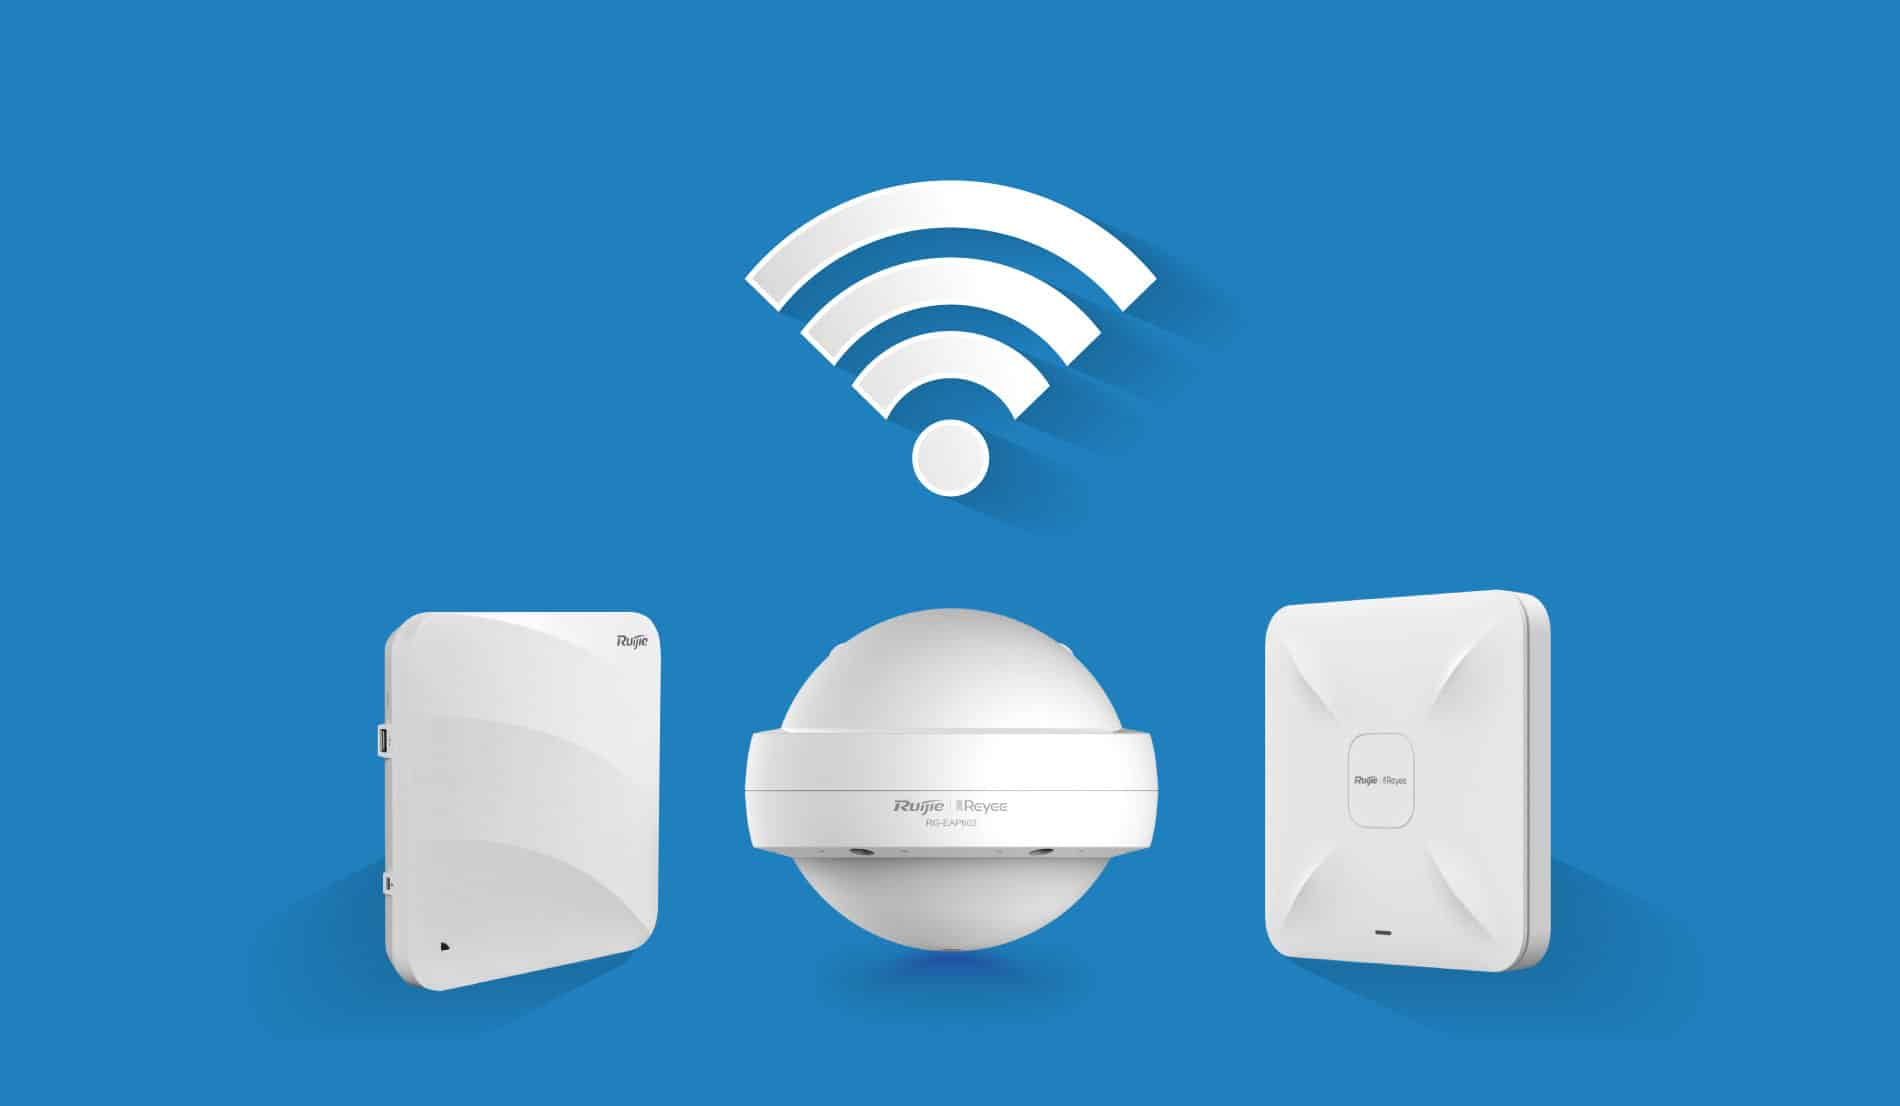
\includegraphics[width=0.85\textwidth]{2/figures/accesspoints.jpg}
		\caption[Access Points]{Access Points.\\
			Fuente: \cite{ot_cisco2024queesap}. \citetitle{ot_cisco2024queesap}.}
		\label{2:fig52}
	\end{center}
\end{figure}

Se pueden configurar para una variedad de funciones según nuestras necesidades. Algunas de las características incluyen:

\begin{itemize}
	\item \textbf{Modo cliente}: Se utiliza como receptor y se conecta a una red como un cable de red. \parencite{ot_ymant2023ap}
	\item \textbf{Modo AP (punto de Acceso)}: El punto de acceso es donde se instala el cableado y permite que varios usuarios accedan a la red. \parencite{ot_ymant2023ap}
	\item \textbf{Modo Repetidor}: Este modo puede extender la señal para que el punto de acceso amplifique la señal que recibe para maximizar el rango de acción. \parencite{ot_ymant2023ap}
	\item \textbf{Modo Bridge}: Este método se emplea para cubrir distancias considerables, como dos edificios distintos. Podemos establecer una red Wi-Fi a distancias significativas si conectamos dos puntos de acceso entre sí. \parencite{ot_ymant2023ap}
\end{itemize}

Los WAP conectan cada dispositivo a la red de manera más fácil, segura y económica que los cables. El uso de WAP para establecer una red inalámbrica puede ser muy ventajoso para las pequeñas empresas. Las redes inalámbricas facilitan el acceso y la incorporación de nuevos usuarios. Con una contraseña segura para la red inalámbrica, un invitado puede acceder fácilmente a Internet. También es posible dividir a los usuarios, incluidos los invitados, para proteger los recursos y los activos de la red. \parencite{ot_cisco2024queesap}

\begin{figure}[!ht]
	\begin{center}
		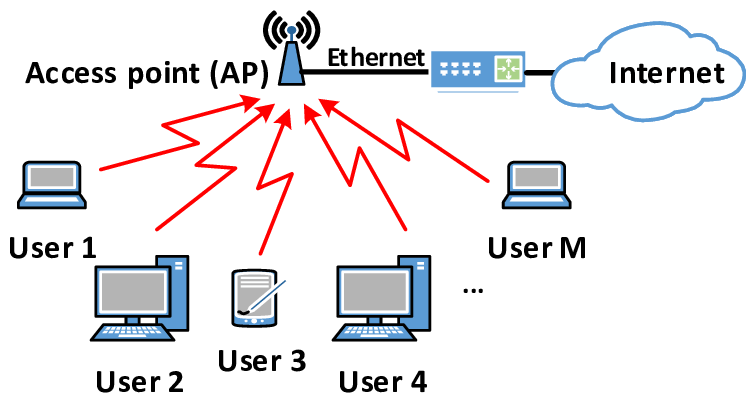
\includegraphics[width=0.85\textwidth]{2/figures/funcionap.png}
		\caption[Funcionamiento de un AP]{Funcionamiento de un AP.\\
			Fuente: \cite{ot_ymant2023ap}. \citetitle{ot_ymant2023ap}.}
		\label{2:fig53}
	\end{center}
\end{figure}



%\chapter{Metodología de la Investigación}
\section{Diseño de la investigación}
En esta sección se detallan el diseño, tipo y enfoque de la investigación, así como la población y la muestra.

\subsection{Tipo de investigación}
Se ha identificado que este estudio posee un diseño experimental con el propósito de establecer el tipo de investigación. Como lo dice \cite{bk_hernandez2014metodologia}, en la obra titulada \citetitle{bk_hernandez2014metodologia}, busca determinar la consecuencia de una razón manipulada. Específicamente, se clasifica como un diseño experimental puro debido a la utilización intencionada de variables independientes (modificadas, eliminadas o añadidas) para evaluar su influencia en la variable dependiente, que en este caso es la predicción de las ubicaciones de puntos de acceso (AP) en diversos planos.

\subsection{Enfoque de la investigación}
Este estudio adoptó un enfoque cuantitativo, conforme a lo explicado por \cite{bk_hernandez2014metodologia} en su libro \citetitle{bk_hernandez2014metodologia}. Este enfoque se basa en la recopilación de datos para comprobar hipótesis mediante mediciones numéricas y análisis estadísticos, con el objetivo de identificar patrones de comportamiento y validar teorías. La metodología empleada sigue los diez pasos del proceso cuantitativo descritos por el autor, aplicados desde la formulación de la idea hasta la presentación de los resultados finales en el informe de investigación.

\subsection{Población}
Podemos mostrar que la población se compone por los diversos entornos y espacios interiores (planos de edificios, oficinas, centros comerciales, etc.) donde se planea optimizar la cobertura de redes inalámbricas mediante la predicción de ubicaciones para puntos de acceso (APs) utilizando Inteligencia Artificial Generativa.

\subsection{Muestra}
La muestra consistió en 19,154 imágenes de planos interiores en formato vectorial del antecedente \cite{art_wu2019interior}, que se obtuvieron del conjunto RPLAN público. El criterio de selección de esta categoría se basó en los problemas que enfrentan tanto empresas como usuarios en la actualidad con la cobertura Wi-Fi y la ubicación ineficaz de los puntos de acceso interior, lo que resulta en quejas y pérdidas de dinero al realizar una reinstalación o reubicación de estos puntos.

\subsection{Operacionalización de Variables}
Los detalles acerca de cómo se definen y miden las variables de estudio se presentan en la Tabla 1.
%\begin{table}[h!]

\begin{longtable}{>{\raggedright\arraybackslash}m{3cm} >{\raggedright\arraybackslash}m{2cm} >{\raggedright\arraybackslash}m{2cm} >{\raggedright\arraybackslash}m{3cm} >{\raggedright\arraybackslash}m{2cm} >{\raggedright\arraybackslash}m{2.5cm}}
    \caption{Matriz de Variables Principales.}
    \label{tabla:variables}\\
    \hline
    VARIABLE & DIMENSIÓN & INDICADOR & DEFINICIÓN DEL INDICADOR & TÉCNICA DE MEDICIÓN & ESCALA \\
    \hline
    Independiente: Imágenes de Planos Interiores & Calidad de la Imagen & Resolución & Número de píxeles por unidad de área (píxeles por pulgada) & Análisis de propiedades de la imagen & ppi (píxeles por pulgada) \\
    \cline{2-6}
     & Detalle Arquitectónico & Número de Elementos Arquitectónicos Identificables & Cantidad de detalles arquitectónicos (paredes, puertas, ventanas) claramente identificables en la imagen & Contaje manual o mediante software de análisis de imágenes & Número \\
    \hline
    Dependiente: Predicción de Ubicaciones de APs Indoor Con Inteligencia Artificial Generativa & Precisión de la Predicción & Diferencia de Cobertura Predicha vs Real & Diferencia entre la cobertura predicha por el algoritmo y la cobertura real medida & Comparación de resultados de simulación y medición real & Porcentaje \\
    \cline{2-6}
     & Sensibilidad & Tasa de Verdaderos Positivos & Proporción de ubicaciones predichas correctamente como óptimas respecto al total de ubicaciones óptimas reales & Evaluación de predicciones respecto a un conjunto de prueba & Porcentaje \\
    \cline{2-6}
     & Puntaje F1 & Media Armónica de Precisión y Sensibilidad & Integra la precisión y la sensibilidad en un único valor & Evaluación de predicciones respecto a un conjunto de prueba & Valor F1 \\
    \cline{2-6}
     & Área Bajo la Curva ROC & AUC-ROC & Evalúa la habilidad del modelo para distinguir entre diferentes clases & Evaluación de la curva ROC & Valor AUC \\
    \hline
\end{longtable}
%\par	%%Salto de linea
%\bigskip
\begin{flushleft}	%%Alinear a la izquierda sin justificar
	\small Fuente: Elaboración propia.
\end{flushleft}
%\end{table}

\section{Técnicas de recolección de datos}
La recolección de planos interiores es un paso crucial para la optimización de la cobertura de redes inalámbricas mediante la Inteligencia Artificial Generativa. Una de las técnicas más accesibles y efectivas para obtener estos planos es a través del uso de bases de datos públicas y repositorios en línea. Estas fuentes ofrecen una amplia variedad de planos de planta, que pueden ser utilizados para modelar y predecir las ubicaciones óptimas de puntos de acceso (APs) en diferentes entornos interiores.

\begin{figure}[h]
	\begin{center}
		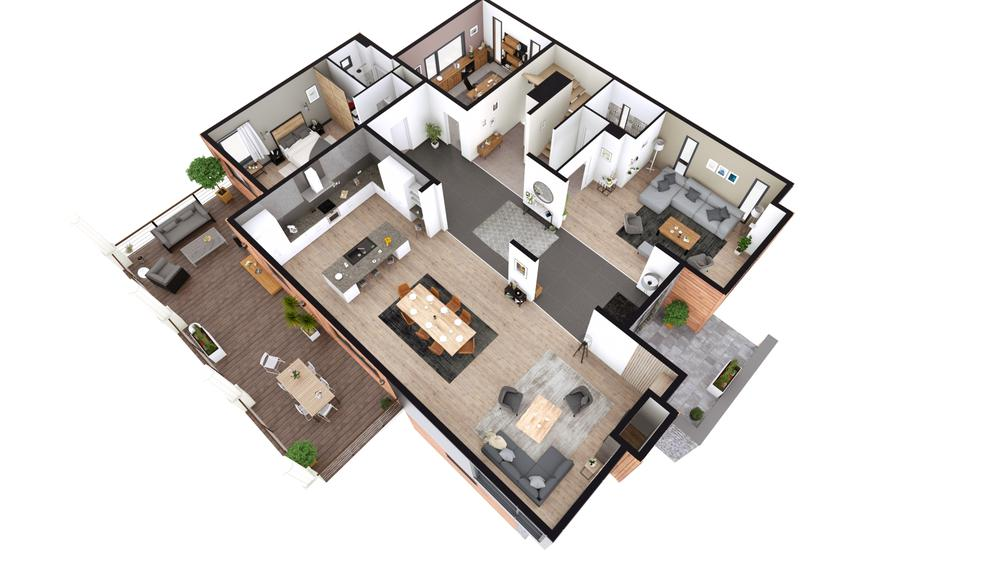
\includegraphics[width=0.75\textwidth]{3/figures/plano2d.jpg}
		\caption[Plano interior]{Plano interior.\\
			Fuente: \cite{art_wu2019interior}.}
		\label{3:fig1}
	\end{center}
\end{figure}

\begin{itemize}
    \item \textbf{Repositorios de Arquitectura y Diseño}: Existen múltiples repositorios en línea dedicados específicamente a la arquitectura y el diseño. Sitios web como ArchDaily, Floorplanner y otros, ofrecen planos de planta y modelos 3D de edificios que pueden ser descargados y utilizados para diversos fines. Estos repositorios suelen incluir planos de diferentes tipos de edificios, desde residenciales hasta comerciales y educativos, lo que proporciona una amplia gama de opciones para la optimización de redes inalámbricas.
    \item \textbf{Bibliotecas Digitales y Bases de Datos Académicas}: Las bibliotecas digitales y bases de datos académicas son otra fuente valiosa para la recolección de planos interiores. Instituciones académicas y bibliotecas públicas a menudo mantienen colecciones de planos de edificios históricos y contemporáneos. Plataformas como JSTOR, Google Scholar y las bibliotecas digitales universitarias pueden contener planos de planta detallados en publicaciones académicas, tesis y proyectos de investigación.
    \item \textbf{Plataformas de Colaboración y Repositorios de Código Abierto}: Plataformas como GitHub y otros repositorios de código abierto también pueden ser recursos útiles para la recolección de planos interiores. Investigadores y profesionales de la industria a menudo comparten conjuntos de datos, modelos y planos como parte de sus proyectos de colaboración. Estos recursos pueden ser utilizados libremente bajo licencias abiertas, lo que facilita su integración en proyectos de optimización de redes inalámbricas.
    \item \textbf{Repositorios de Proyectos de Construcción}: Sitios web como Procore y otros repositorios de gestión de proyectos de construcción ofrecen planos y documentos relacionados con proyectos de construcción. Estos repositorios son utilizados por profesionales de la construcción para gestionar y compartir información sobre proyectos, y a menudo incluyen planos de planta detallados que pueden ser utilizados para análisis posteriores.
    \end{itemize}



%\newpage
\section{Técnicas para el procesamiento y análisis de la información}

\subsection{Metodología de implementación de la solución}

La producción de imágenes mediante Inteligencia Artificial Generativa involucra varias fases de desarrollo, que van desde la recopilación de imágenes hasta su interpretación, como se menciona en el trabajo de \cite{tec_kingma2019variat}. La imagen adquirida debe pasar por un proceso detallado posteriormente para alcanzar su etapa final. La metodología de esta investigación se muestra en la Figura 37.

\begin{figure}[h]
	\begin{center}
		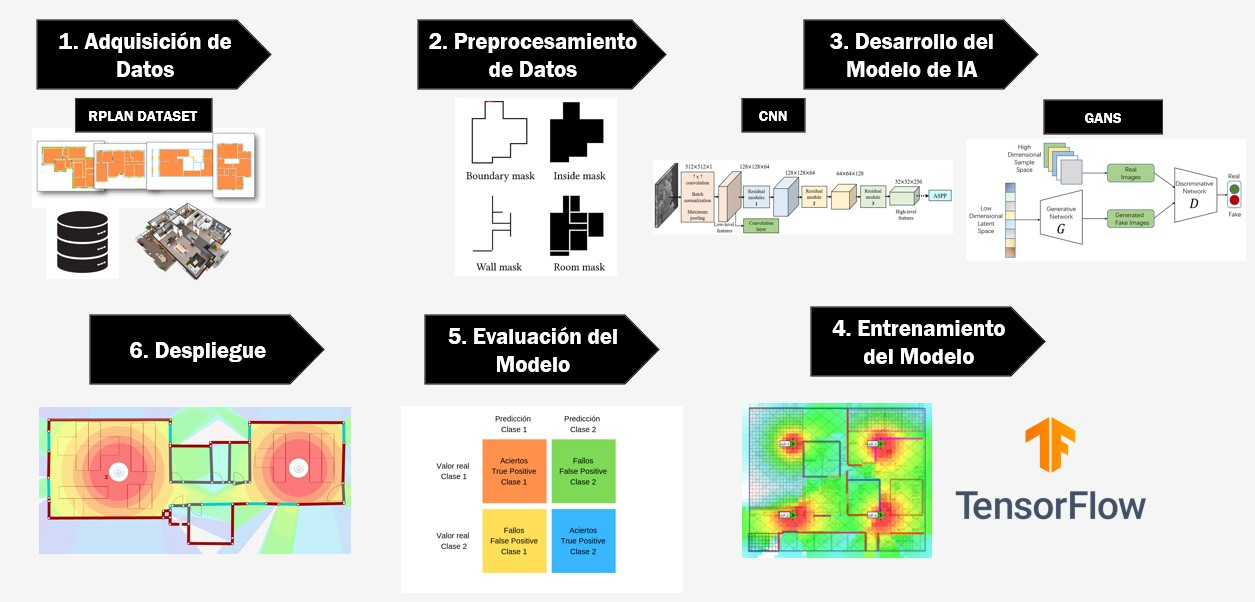
\includegraphics[width=1.1\textwidth]{3/figures/metodologia.jpg}
		\caption[Método de Investigación]{Método de Investigación.\\
			Fuente: Elaboración propia.}
		\label{3:fig2}
	\end{center}
\end{figure}

\newpage
\subsubsection{Adquisición de Datos}

En esta sección se describe el procedimiento utilizado para obtener el conjunto de datos empleado en este estudio. A continuación, se presenta una tabla que resume las tareas y actividades realizadas durante esta fase de adquisición. El primer paso fue la recopilación de datos. Los detalles sobre las actividades y tareas se encuentran en la Tabla 2.

\begin{longtable}{>{\raggedright\arraybackslash}p{4cm} >{\raggedright\arraybackslash}p{4cm} >{\raggedright\arraybackslash}p{5cm}}
    \caption{Tabla de la Adquisición de Datos.}
    \label{tabla:actividades}\\
    \hline
    \textbf{Actividades} & \textbf{Descripción} & \textbf{Tareas}\\
    \hline
    \endfirsthead

    \multicolumn{3}{c}%
    {{\bfseries \tablename\ \thetable{} -- continuación de la página anterior}} \\
    \hline
    \textbf{Actividades} & \textbf{Descripción} & \textbf{Tareas}\\
    \hline
    \endhead

    \hline
    \multicolumn{3}{r}{{Continúa en la siguiente página}} \\
    \endfoot

    \hline
    \endlastfoot

    Identificación de la data que contengan imágenes de planos interiores de planta con dimensiones idénticas y características similares. & Identificación de la data que contengan imágenes de planos interiores de planta relevantes para la investigación. & 
    \begin{itemize}
        \item Analizar y identificar bases de datos con planos de planta interiores.
        \item Confirmar que la base de datos esté disponible públicamente y sea pertinente para el estudio.
        \item Descargar los datos desde el repositorio apropiado.
    \end{itemize} \\
\end{longtable}


\begin{flushleft}
    \small Fuente: Elaboración propia.
\end{flushleft}

Enseguida, se proporciona un detalle de la actividad mencionada en la tabla anterior, junto con los resultados que se esperan obtener.

\textbf{Actividad 1: Identificación de la data que contengan imágenes de planos interiores de planta con dimensiones idénticas y características similares}
\\
Esta actividad explica la identificación de la data. Para la data, se obtuvieron más de ochenta mil planos de plantas de edificios residenciales reales de la data pública RPLAN, que recolectó planos del mercado inmobiliario de Asia en 2019. Las imágenes de planos interiores se encuentran en la base de datos. La Figura 38 muestra ejemplos de cómo es la data. Cada plano de planta tiene gráficos vectoriales dentro de una región cuadrada de 18m × 18m con elementos geométricos e información semántica, y cada plano de planta tiene una imagen de 256 × 256.


\textbf{Entregable}: Dataset, creado en Asia, contiene imágenes de planos interiores del mercado inmobiliario asiático.


\subsubsection{Preprocesamiento de Datos}
Se realizará el preprocesamiento de las imágenes del conjunto en esta etapa. La tabla 3 incluye las tareas y actividades necesarias para completar la etapa de preprocesamiento:
\vspace{2ex}


\begin{longtable}{|p{3cm}|p{3cm}|p{9cm}|}
    \caption{Actividades de la fase de Preprocesamiento de Datos.}
    \label{tabla:preprocesamiento}\\
    \hline
    \textbf{Actividades} & \textbf{Descripción} & \textbf{Tareas} \\
    \hline
    \endfirsthead

    \hline
    \textbf{Actividades} & \textbf{Descripción} & \textbf{Tareas} \\
    \hline
    \endhead

    \hline
    \endfoot

    \hline
    \endlastfoot

    Filtración de las imágenes de los planos interiores& Filtrado de datos no estándar para evitar interferencias y mejorar la fiabilidad del conjunto de datos. & 
    \begin{itemize}
        \item Eliminar planos de planta que contengan tipos de habitaciones indefinidas o de muy baja frecuencia.
        \item Mantener planos de planta que cumplan con los siguientes requisitos:
        \begin{enumerate}
            \item Área total del plano de planta superior a 60 m² y menor a 120 m².
            \item Número de habitaciones en el plano de planta mayor que 3 y menor que 9.
            \item El plano de planta tiene sala de estar.
            \item La proporción del área de la sala de estar respecto al área total del plano de planta es mayor que 0.25 y menor que 0.55.
            \item El área promedio de cada habitación es mayor a 10 m² y menor a 20 m².
        \end{enumerate}
    \end{itemize} \\
    \hline
    Representación de las imágenes de los planos interiores& Representación de cada plano de planta como una imagen de cuatro canales. & 
    \begin{itemize}
        \item Guardar la máscara interior en el primer canal.
        \item Almacenar la información de límites en el segundo canal.
        \item Representar la semántica de habitaciones y paredes en el tercer canal con números enteros específicos.
        \item Usar el cuarto canal para almacenar información adicional que distinga entre diferentes habitaciones con las mismas etiquetas. Diferentes números enteros se utilizan para distinguir habitaciones con las mismas etiquetas.
    \end{itemize} \\
    \hline
    \caption{Actividades de la fase de Preprocesamiento de Datos.}
    \label{tabla:actividades}
\end{longtable}


%\par	%%Salto de linea
%\bigskip
\begin{flushleft}	%%Alinear a la izquierda sin justificar
	\small Fuente: Elaboración propia.
\end{flushleft}

Enseguida, se describe en detalle las actividades junto con el resultado esperado.

\textbf{Actividad 1: Filtración de las imágenes de los planos interiores}
\\
En la fase de preprocesamiento de datos, la actividad de Filtración se enfoca en depurar y mejorar la calidad del conjunto de datos al eliminar información irrelevante o poco confiable. Esto se logra a través de la eliminación de datos no estándar y la conservación de aquellos que cumplen con criterios específicos de relevancia y fiabilidad. 

\textbf{Entregable}: Conjunto de datos filtrado y optimizado para su posterior análisis.

\textbf{Actividad 2: Representación de las imágenes de los planos interiores}
\\
Por otro lado, la actividad de Representación se encarga de convertir los datos en un formato visual o estructurado más adecuado para su análisis y comprensión. Esto implica transformar los datos en imágenes o representaciones gráficas que faciliten su visualización y entendimiento, contribuyendo así a una mejor interpretación por parte de los usuarios finales, como podemos observar en la Figura 38.

\textbf{Entregable}: Representación visual y estructurada de cada plano de planta en un formato adecuado para su procesamiento y análisis posterior.

\begin{figure}[h]
    \begin{center}
        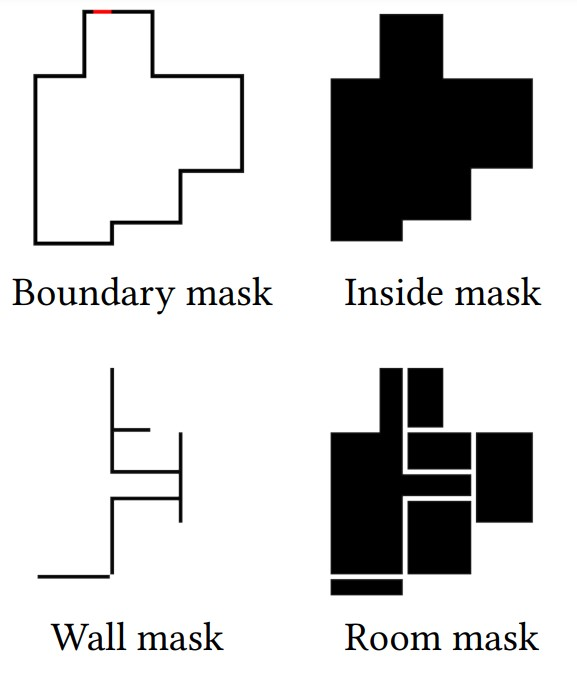
\includegraphics[width=0.5\textwidth]{3/figures/Representacion_planos.jpg}
        \caption[Representación de las imágenes de los planos interiores]{Representación de las imágenes de los planos interiores.\\
        Fuente: \cite{art_wu2019interior}. \citetitle{art_wu2019interior}.}
        \label{3:fig3}
    \end{center}
\end{figure}

\subsubsection{Desarrollo del Modelo de IA}
Tres actividades fundamentales componen el modelo generativo para la optimización de la cobertura de las redes inalámbricas para la predicción de las ubicaciones de los puntos de acceso. Cada una de estas actividades utiliza estrategias de Aprendizaje Profundo avanzadas para trabajar de manera secuencial y colaborativa. La Tabla 4 muestra todo esto más a fondo.

\vspace{2ex}
\begingroup
\renewcommand\arraystretch{0.3}
\begin{longtable}{|p{4cm}|p{6cm}|p{6cm}|}
    \caption{Actividades de la fase de Desarrollo del Modelo de IA.}
    \label{tabla:actividades}\\
    \hline
    \textbf{Actividades} & \textbf{Descripción} & \textbf{Tareas} \\
    \hline
    \endfirsthead
    
    \multicolumn{3}{c}%
    {{\bfseries \tablename\ \thetable{} -- continuación de la página anterior}} \\
    \hline
    \textbf{Actividades} & \textbf{Descripción} & \textbf{Tareas} \\
    \hline
    \endhead
    
    \hline \multicolumn{3}{|r|}{{Continúa en la próxima página}} \\
    \hline
    \endfoot
    
    \hline
    \endlastfoot
    
    Arquitectura de la Red & Diseñar la arquitectura de la red neuronal para la predicción de APs. & 
    \begin{itemize}
        \item Selección del tipo de red CNN y GAN.
        \item Diseño de la arquitectura de la red (capas convolucionales).
        \item Implementación de la red en un framework de Aprendizaje Profundo.
        \item Definición de entradas y salidas.
    \end{itemize} \\
    \hline
    
    \end{longtable}
\endgroup

%\par	%%Salto de linea
%\bigskip
\begin{flushleft}	%%Alinear a la izquierda sin justificar
	\small Fuente: Elaboración propia
\end{flushleft}

Enseguida, se proporciona un detalle de la actividad junto con el entregable correspondiente que se espera obtener.

\textbf{Actividad 1: Arquitectura de la Red}
\\
Durante esta etapa, mencionaré el diseño e implementación de la arquitectura de una red neuronal destinada a predecir las ubicaciones de puntos de acceso (APs). Se empleará una combinación de Redes Neuronales Convolucionales (CNN) y Redes Generativas Antagónicas (GANs) para aprovechar sus capacidades en la extracción de características espaciales y la generación de soluciones óptimas.

Respecto, al proceso de Red Neuronal Convolucional (CNN) para la extracción de características, podemos verla con más detalle en la Figura 39, donde se ve el uso de la capa Conv2D (Varias capas convolucionales para extraer características espaciales), la capa MaxPooling2D (Capas de pooling para reducir dimensionalidad y mantener características importantes), la capa Flatten (Aplanar la salida para conectarla con capas densas) y finalmente la capa Dense (Capas densas para aprendizaje y combinación de características extraídas).

\begin{figure}[H]
	\centering
	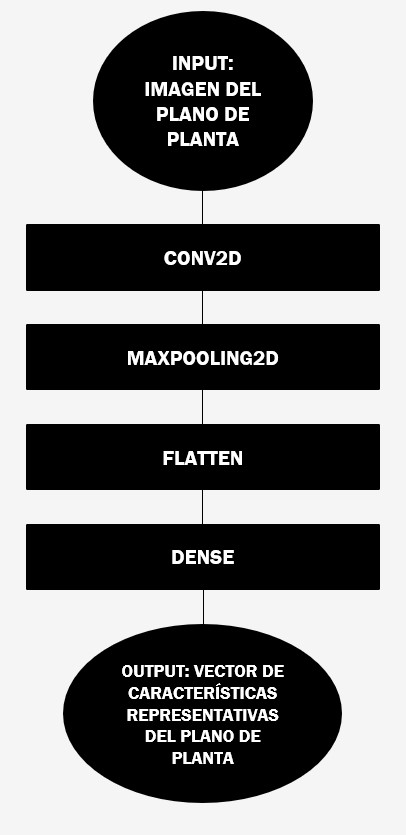
\includegraphics[width=0.3\textwidth]{3/figures/CNN_redneuro.jpg}
	\caption[CNN para el análisis y extracción de rasgos característicos]{CNN para el análisis y extracción de rasgos característicos.\\ Fuente: Elaboración propia.}
	\label{3:4}
\end{figure}


Por consiguiente, al proceso del Generador del GAN, podemos verla con más detalle en la Figura 40, donde se ve el uso de la capa Dense (Varias capas densas para transformar el vector de características en un plano con las ubicaciones de los Aps), la capa Reshape (Dar forma al plano para que corresponda con las dimensiones del plano de planta), la capa Flatten (Aplanar la salida para conectarla con capas densas) y finalmente la capa Conv2DTranspose (Capas convolucionales transpuestas para generar la imagen final).

\begin{figure}[H]
	\centering
	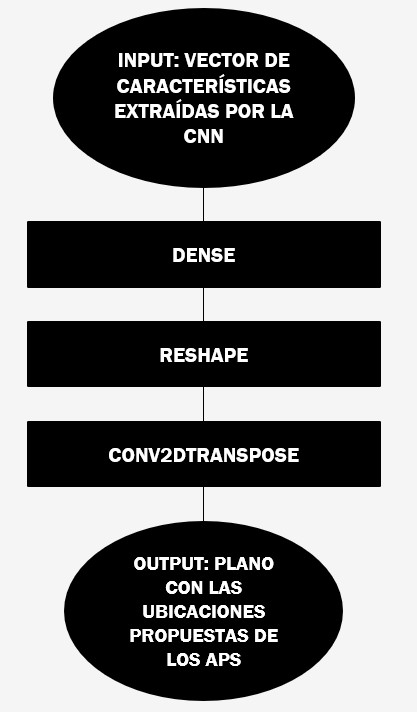
\includegraphics[width=0.4\textwidth]{3/figures/gans_capas.jpg}
	\caption[Generador del GAN]{Generador del GAN.\\ Fuente: Elaboración propia.}
	\label{3:5}
\end{figure}

Finalmente, al proceso del Discriminador del GAN, podemos verla con más detalle en la Figura 41, donde se ve el uso de la capa Conv2D (Varias capas convolucionales para analizar la imagen y evaluar la calidad de las ubicaciones propuestas), la capa MaxPooling2D (Capas de pooling para reducir dimensionalidad), la capa Flatten (Aplanar la salida para conectarla con capas densas) y finalmente la capa Dense (Capas densas para la clasificación final).

\begin{figure}[H]
	\centering
	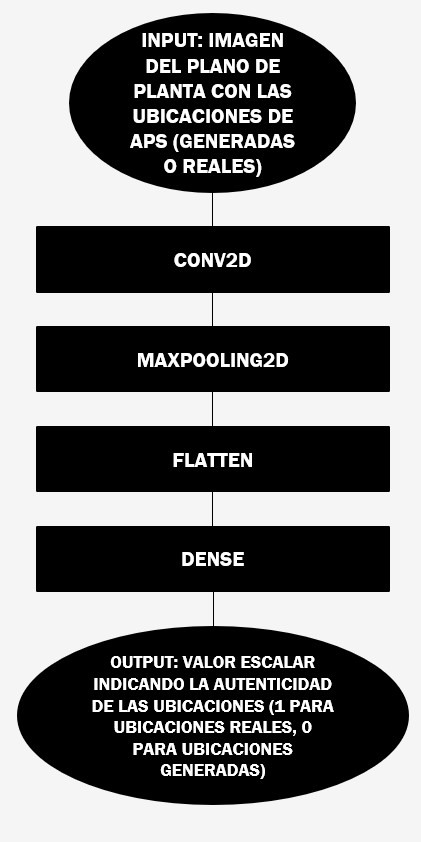
\includegraphics[width=0.4\textwidth]{3/figures/discrimGAN.jpg}
	\caption[Discriminador del GAN]{Discriminador del GAN.\\ Fuente: Elaboración propia.}
	\label{3:6}
\end{figure}

A todo ello se se utilizará TensorFlow para implementar la arquitectura descrita. A continuación, se presenta un pseudocódigo para la implementación en la Figura 42.

\begin{figure}[H]
	\centering
	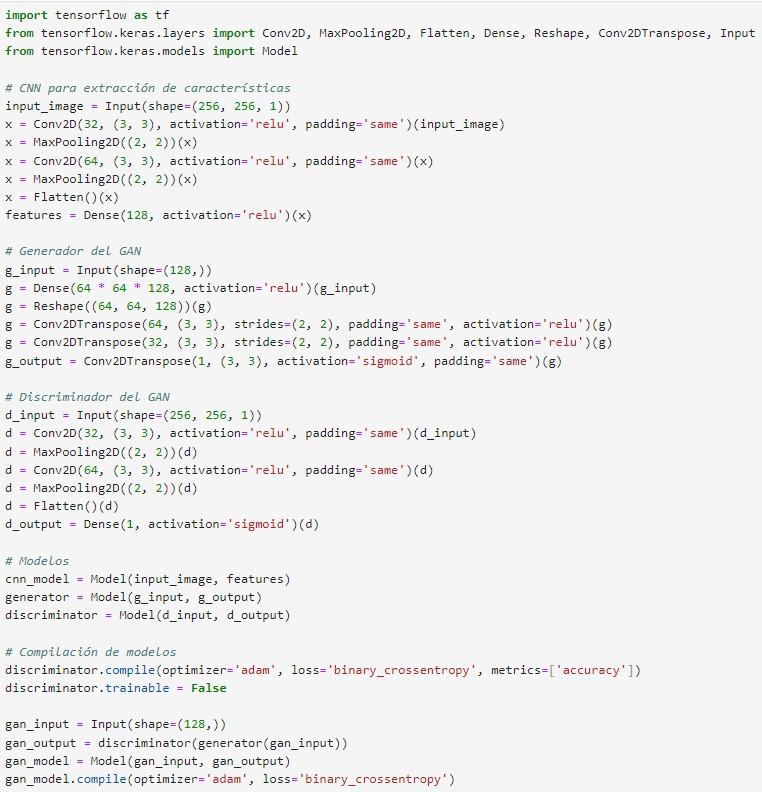
\includegraphics[width=1\textwidth]{3/figures/pseudocodigo.jpg}
	\caption[Pseudocódigo para la implementación]{Pseudocódigo para la implementación.\\ Fuente: Elaboración propia.}
	\label{3:7}
\end{figure}

\textbf{Entregable}: Código fuente de la red neuronal implementada, Diagramas y especificaciones de la arquitectura de la red y Especificaciones de entrada y salida del modelo.

\subsubsection{Entrenamiento del Modelo}
Al concluir la etapa del Desarrollo del Modelo de IA, se continua con el Entrenamiento, en la Tabla 5 fueron diseñados siguiendo las actividades.

\vspace{2ex}
\begingroup
\renewcommand\arraystretch{0.3}
\begin{longtable}{|p{4cm}|p{6cm}|p{6cm}|}
    \caption{Actividades del Entrenamiento del Modelo.}
    \label{tabla:actividades}\\
    \hline
    \textbf{Actividades} & \textbf{Descripción} & \textbf{Tareas} \\
    \hline
    \endfirsthead
    
    \multicolumn{3}{c}%
    {{\bfseries \tablename\ \thetable{} -- continuación de la página anterior}} \\
    \hline
    \textbf{Actividades} & \textbf{Descripción} & \textbf{Tareas} \\
    \hline
    \endhead
    
    \hline \multicolumn{3}{|r|}{{Continúa en la próxima página}} \\
    \hline
    \endfoot
    
    \hline
    \endlastfoot
    
    Entrenamiento Supervisado & Utilizar datos anotados para entrenar el modelo de predicción de APs. & 
    \begin{itemize}
        \item Entrenamiento del modelo utilizando el dataset anotado.
        \item Evaluación y ajuste de hiperparámetros.
    \end{itemize} \\
    \hline
    
    Optimización de Cobertura & Entrenar el modelo para maximizar la cobertura y minimizar la interferencia. & 
    \begin{itemize}
        \item Uso de técnicas de regularización para evitar sobreajuste.
        \item Simulaciones para evaluar el impacto de las predicciones de APs en la cobertura de red.
        \item Ajuste iterativo del modelo basado en los resultados de las simulaciones.
    \end{itemize} \\
    \hline
    
    \end{longtable}
\endgroup

\textbf{Actividad 1: Entrenamiento Supervisado}
\\
El entrenamiento supervisado implica el uso de un conjunto de datos anotado donde las ubicaciones óptimas de los puntos de acceso (APs) están previamente definidas. Este proceso es fundamental para enseñar al modelo a reconocer patrones y aprender a predecir ubicaciones óptimas de APs en base a la disposición de los planos de planta.
Asimismo, se elaboró el pseudocódigo el cual se puede ver en la Figura 43.

\begin{figure}[H]
	\centering
	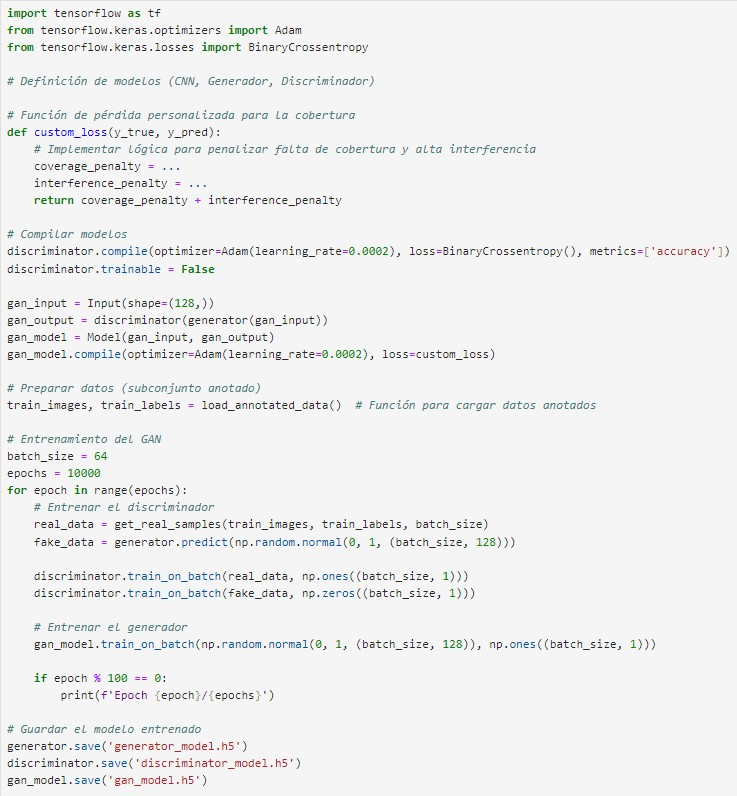
\includegraphics[width=1\textwidth]{3/figures/pseudo_train.jpg}
	\caption[Pseudocódigo para el Entrenamiento Supervisado]{Pseudocódigo para el Entrenamiento Supervisado.\\ Fuente: Elaboración propia.}
	\label{3:8}
\end{figure}

\textbf{Entregable}: Modelo entrenado y archivos de checkpoints.

\textbf{Actividad 2: Optimización de Cobertura}
\\
La optimización de la cobertura implica ajustar el modelo para maximizar la cobertura de red y minimizar la interferencia. Esto se logra implementando métricas específicas en la función de pérdida y realizando simulaciones de cobertura.

Asimismo, se elaboró el pseudocódigo el cual se puede ver en la Figura 44.

\begin{figure}[H]
	\centering
	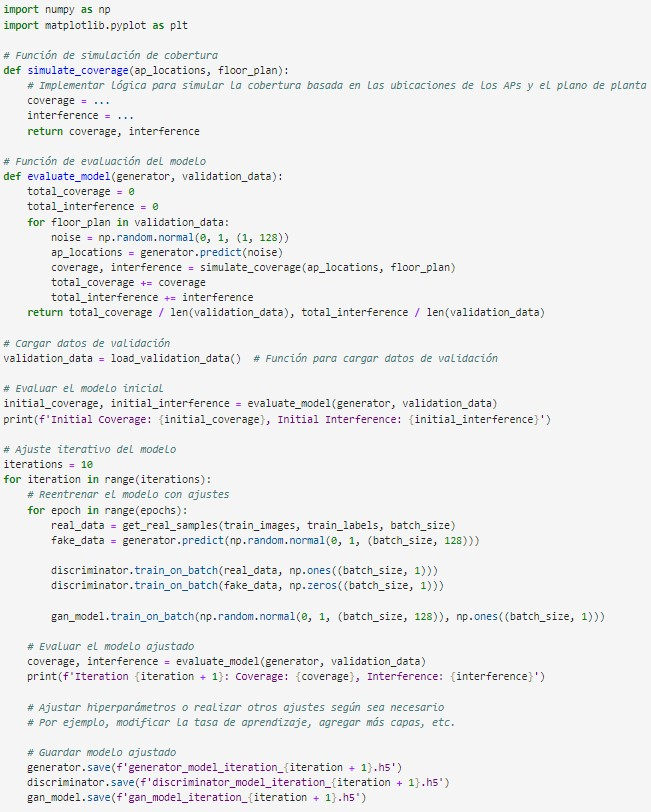
\includegraphics[width=1\textwidth]{3/figures/pseudo_cobert.jpg}
	\caption[Pseudocódigo para la Optimización de Cobertura]{Pseudocódigo para la Optimización de Cobertura.\\ Fuente: Elaboración propia.}
	\label{3:9}
\end{figure}

\textbf{Entregable}: Función de pérdida mejorada con métricas de cobertura e interferencia y Reporte de resultados de simulaciones de cobertura.

\subsubsection{Evaluación del Modelo}
Durante esta fase, se procede a evaluar los modelos desarrollados en la investigación utilizando las métricas de clasificación seleccionadas y descritas en la sección 3.3.2. La Tabla 6 proporciona un desglose detallado de las actividades y tareas realizadas durante esta fase.

%\vspace{2ex}
%\begingroup
%\renewcommand\arraystretch{0.3}
\begin{longtable}{|>{\raggedright\arraybackslash}p{4cm}|>{\raggedright\arraybackslash}p{5cm}|>{\raggedright\arraybackslash}p{6cm}|}
    \caption{Actividades de la Evaluación del Modelo.}
    \label{tabla:actividades}\\
    \hline
    \textbf{Actividad} & \textbf{Descripción} & \textbf{Tareas} \\
    \hline
    \endfirsthead

    \hline
    \textbf{Actividad} & \textbf{Descripción} & \textbf{Tareas} \\
    \hline
    \endhead

    \hline
    \endfoot

    \hline
    \endlastfoot

    Preparación de Datos de Validación & Seleccionar y preparar un conjunto de datos de validación representativo. & 
    \begin{itemize}
        \item Elección de planos de planta que no hayan sido empleados en el proceso de entrenamiento.
        \item Preprocesamiento de imágenes.
    \end{itemize} \\
    \hline
    Definición de Métricas de Evaluación & Definir métricas cuantitativas para evaluar la cobertura y la interferencia. & 
    \begin{itemize}
        \item Identificación de métricas adecuadas.
        \item Implementación de funciones para calcular estas métricas.
    \end{itemize} \\
    \hline
    Evaluación del Modelo & Evaluar el modelo entrenado en el conjunto de datos de validación para obtener una línea base. & 
    \begin{itemize}
        \item Predicción de ubicaciones de APs en el conjunto de validación.
        \item Cálculo de métricas de evaluación.
    \end{itemize} \\
    \hline
\end{longtable}
%\endgroup
%\par	%%Salto de linea
%\bigskip
\begin{flushleft}	%%Alinear a la izquierda sin justificar
	\small Fuente: Elaboración propia
\end{flushleft}

\textbf{Actividad 1: Preparación de Datos de Validación}
\\
La preparación de los datos de validación desempeña un papel crucial en la evaluación de la efectividad del modelo en datos no previamente vistos. Esta tarea implica seleccionar un subconjunto representativo del conjunto de datos que no se haya utilizado durante el entrenamiento del modelo. La selección debe tener en cuenta la diversidad en los planos de planta y sus configuraciones para garantizar que el modelo pueda generalizar correctamente a diferentes escenarios.

\textbf{Entregable}: Un conjunto de datos listo para su uso en la evaluación del modelo, que incluye imágenes preprocesadas y listas para ser utilizadas en el análisis.

\textbf{Actividad 2: Definición de Métricas de Evaluación}
\\
Para evaluar el rendimiento del modelo de manera cuantitativa, es esencial definir métricas claras que reflejen tanto la cobertura de la red como los niveles de interferencia. Estas métricas proporcionarán una base objetiva para comparar el rendimiento del modelo en diferentes escenarios y con otros enfoques existentes.

\textbf{Entregable}: Un documento detallado que describe cada métrica y proporciona el código o las funciones necesarias para calcularlas.

\vspace{0.5cm}
\textbf{Actividad 3: Evaluación del Modelo}
\\
La evaluación del modelo involucra el uso del conjunto de datos de validación para establecer un punto de referencia sobre su rendimiento. Esta evaluación es esencial para comprender el comportamiento del modelo en situaciones no previamente vistas durante el entrenamiento y para identificar posibles áreas de mejora.

\textbf{Entregable}: Un informe que presenta los resultados de la evaluación inicial, incluyendo las métricas de rendimiento calculadas y cualquier observación relevante sobre el comportamiento del modelo.

\subsubsection{Despliegue}
Al concluir la metodología empleada, se procedió a implementar el modelo propuesto luego de finalizar su entrenamiento y evaluación correspondiente. Los pasos y tareas realizados en esta fase se encuentran detallados en la Tabla 7.

%\vspace{2ex}
%\begingroup
%\renewcommand\arraystretch{0.3}
\begin{longtable}{|>{\raggedright\arraybackslash}p{4cm}|>{\raggedright\arraybackslash}p{5cm}|>{\raggedright\arraybackslash}p{6cm}|}
    \caption{Actividades del Despliegue.}
    \label{tabla:actividades}\\
    \hline
    \textbf{Actividad} & \textbf{Descripción} & \textbf{Tareas} \\
    \hline
    \endfirsthead

    \hline
    \textbf{Actividad} & \textbf{Descripción} & \textbf{Tareas} \\
    \hline
    \endhead

    \hline
    \endfoot

    \hline
    \endlastfoot

    Preparación del Entorno de Despliegue & Configurar el entorno necesario para desplegar el modelo en producción. & 
    \begin{itemize}
        \item Selección de infraestructura.
        \item Configuración del entorno de hardware y software.
        \item Pruebas iniciales.
    \end{itemize} \\
    \hline
    Despliegue del Modelo en Producción & Implementar el modelo en el entorno de producción para su uso real. & 
    \begin{itemize}
        \item Implementación del modelo en producción.
        \item Configuración de parámetros en tiempo de ejecución.
        \item Monitoreo inicial del desempeño.
    \end{itemize} \\
    \hline
\end{longtable}
%\endgroup
%\par	%%Salto de linea
%\bigskip
\begin{flushleft}	%%Alinear a la izquierda sin justificar
	\small Fuente: Elaboración propia
\end{flushleft}

\textbf{Actividad 1: Preparación del Entorno de Despliegue}
\\
La preparación del entorno de despliegue es una etapa fundamental para asegurar que el modelo de IA pueda ser ejecutado eficientemente en producción. Este proceso implica la selección y configuración de la infraestructura necesaria, incluyendo tanto hardware como software, y la realización de pruebas iniciales para confirmar que todo funciona correctamente antes del despliegue completo.

\textbf{Entregable}: Un entorno completamente preparado, con todos los componentes necesarios instalados y configurados, listo para el despliegue del modelo.

\vspace{0.25cm}
\textbf{Actividad 2: Despliegue del Modelo en Producción}
\\
El despliegue del modelo en producción es el paso en el que el modelo de IA se pone en funcionamiento en el entorno de producción. Este proceso incluye la implementación del modelo, la configuración de parámetros necesarios para su ejecución en tiempo real, y el monitoreo inicial para asegurar que el modelo funciona correctamente en condiciones reales.

\textbf{Entregable}: El modelo está completamente implementado y operando en el entorno de producción, con los parámetros ajustados y el desempeño monitoreado para asegurar su correcto funcionamiento.

\vspace{0.5cm}
\subsection{Metodología para la medición de resultados}
Diversas métricas se emplean para evaluar el desempeño de un modelo, sirviendo como herramientas de evaluación fundamentadas en los datos de la Matriz de Confusión. A continuación, se detalla su concepto y sus componentes.

\begin{itemize}
\item \textbf{Matriz de confusión}: La Matriz de Confusión es una tabla de dimensiones NxN que sintetiza la precisión de las predicciones generadas por un modelo de clasificación. Esta matriz muestra la relación entre las etiquetas predichas por el modelo y las etiquetas reales de los datos. Uno de los ejes de la matriz representa las etiquetas predichas, mientras que el otro muestra las etiquetas reales, con N representando el número total de clases. En el contexto de un problema de clasificación binaria, N=2 \parencite{gl_kohavi1998ml_glossary}. Su objetivo principal es evaluar el rendimiento de un modelo de Machine Learning supervisado en datos de prueba, donde las etiquetas reales son desconocidas. El término <<matriz de confusión>> se origina porque ayuda a identificar dónde el sistema confunde entre dos clases (Big Data, 2019). Puedes encontrar una representación visual de la matriz de confusión en la Figura 45.
\begin{figure}[H]
	\centering
	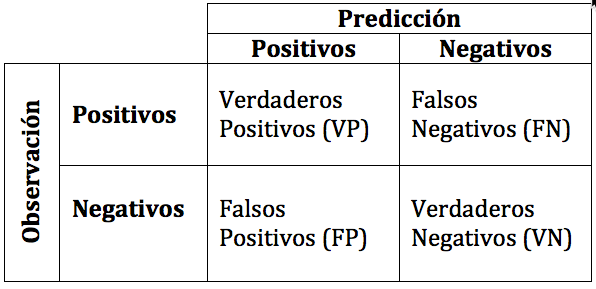
\includegraphics[width=0.75\textwidth]{3/figures/matriz_confusion.png}
	\caption[Matriz de Confusión]{Matriz de Confusión.\\ Fuente: \cite{gl_izco2018bdc}. \citetitle{gl_izco2018bdc}.}
	\label{3:9}
\end{figure}
\end{itemize}

\begin{itemize}
    \item \textbf{Verdaderos Positivos}: Se denomina verdadero positivo cuando el modelo realiza una predicción precisa de la clase positiva.
    \item \textbf{Verdaderos Negativos}: Se trata de un verdadero negativo cuando el modelo realiza una predicción correcta de la clase negativa.
    \item \textbf{Falsos Positivos}: Ocurre un falso positivo cuando el modelo hace una predicción incorrecta de la clase positiva. 
    \item \textbf{Falsos Negativos}: Ocurre un falso negativo cuando el modelo hace una predicción incorrecta de la clase negativa. 
    \end{itemize}

    Después de explicar los conceptos previos, se obtienen las siguientes métricas comúnmente utilizadas en clasificación, de las cuales se utilizarán solo las tres primeras según lo referenciado en los documentos anteriores:

    \begin{itemize}
    \item \textbf{Exactitud}: se determina a partir de la fórmula que se mostrará \parencite{gl_kohavi1998ml_glossary} y cuantifica la precisión de las predicciones en relación con el conjunto total de ejemplos en un modelo de clasificación.
    	%\begin{equcaption}[!ht]
    \begin{equation}\label{eq:accuracy}
        \phantomsection
        Exactitud=\frac{V.P.+V.N.}{V.P.+V.N.+F.P.+F.N.}
        \end{equation}
        \myequations{Fórmula para la exactitud}
        
        La pregunta que responde esta métrica es ¿Cuál es la proporción de predicciones correctas? 
        
        \item \textbf{Precisión}: evalúa la proporción de elementos identificados correctamente como positivos entre todos los elementos identificados como positivos. Su cálculo se basa en la siguiente expresión.
        \begin{equation}\label{eq:precision}
            \phantomsection
            \text{Precisión}=\frac{V.P.}{V.P.+F.P.}
            \end{equation}
        \myequations{Fórmula para la precisión}
        
        La pregunta que responde esta métrica es: ¿Cuál es la proporción de predicciones positivas que son precisas?

	\item \textbf{Área bajo la curva ROC}: es una medida que abarca todos los posibles umbrales de clasificación, indicando la probabilidad de que un clasificador esté más confiado en identificar un verdadero positivo que un falso positivo \parencite{gl_google2018machinelearning}. Para comprender mejor esta métrica, es fundamental tener conocimiento previo sobre la curva ROC y su relevancia en evaluaciones de modelos.
	
    La curva ROC es una herramienta que evalúa la capacidad de distinguir entre dos categorías en un modelo, como por ejemplo, determinar si un paciente tiene cáncer o no.

Al ajustar el umbral hacia la izquierda, lo que aumenta la sensibilidad, la especificidad tiende a disminuir. Por otro lado, al mover el umbral hacia la derecha, disminuye la sensibilidad y aumenta la especificidad. Según \parencite{gl_gonzalez2019auc}, el área bajo la curva (AUC) refleja la sensibilidad en función de la especificidad.

El rendimiento del modelo se refleja en el área bajo la curva, donde un rendimiento superior se evidencia en una curva que se distancia de la diagonal principal. Este cálculo se realiza utilizando la siguiente fórmula:

\begin{equation}\label{eq
}
\phantomsection
\mathrm{P}(\text{score}(x^{+}) > \text{score}(x^{-}))
\end{equation}
\myequations{Fórmula para el área bajo la curva ROC}
En cuanto a la interpretación del AUC, se establece lo siguiente:
\begin{itemize}
    \item Si el valor es igual a 0.5, indica que el modelo no tiene capacidad discriminativa.
    \item Si el valor está entre 0.5 y 0.7, se considera que la capacidad discriminativa del modelo es insatisfactoria.
    \item Si el valor está entre 0.7 y 0.8, se considera que la capacidad discriminativa del modelo es aceptable.
    \item Si el valor está entre 0.8 y 0.9, se considera que la capacidad discriminativa del modelo es excelente.
    \item Si el valor es igual o mayor a 0.9, se considera que la capacidad discriminativa del modelo es excepcionalmente buena.
    \end{itemize}
	\item \textbf{Sensibilidad}: 
    Evalúa la fracción de elementos correctamente detectados como positivos en relación con el número total de positivos verdaderos \parencite{gl_bigdata2019metricas}. Su determinación se efectúa utilizando la siguiente fórmula:

	\begin{equation}\label{eq:recall}
        \phantomsection
        \text{Sensibilidad}=\frac{V.P.}{V.P.+F.N.}
        \end{equation}
        \myequations{Fórmula para la sensibilidad}
        
        \item \textbf{Puntaje F1}: El F1-score es una medida que combina la precisión y la sensibilidad en una media armónica. Se emplea especialmente cuando estas métricas difieren significativamente entre sí, lo que dificulta llegar a una conclusión definitiva debido a que solo se puede predecir de manera precisa una de las clases \parencite{gl_bigdata2019metricas}. Su cálculo se realiza mediante la siguiente fórmula:

        \begin{equation}\label{eq:f1-score}
        \phantomsection
        Puntaje F1=\frac{2*Precisi\acute{o}n*Sensibilidad}{Precisi\acute{o}n+Sensibilidad}
        \end{equation}
        \myequations{Fórmula para el puntaje F1}
	
\end{itemize}

\begin{landscape}
	\section{Cronograma de actividades y presupuesto}
	Se creó un plan de trabajo detallado para el proyecto de investigación, representado en la Figura 46, abarcando desde su inicio a inicios de 2024 hasta la presentación del trabajo prevista para finales de 2024.

	\begin{figure}[!ht]
		\begin{center}
			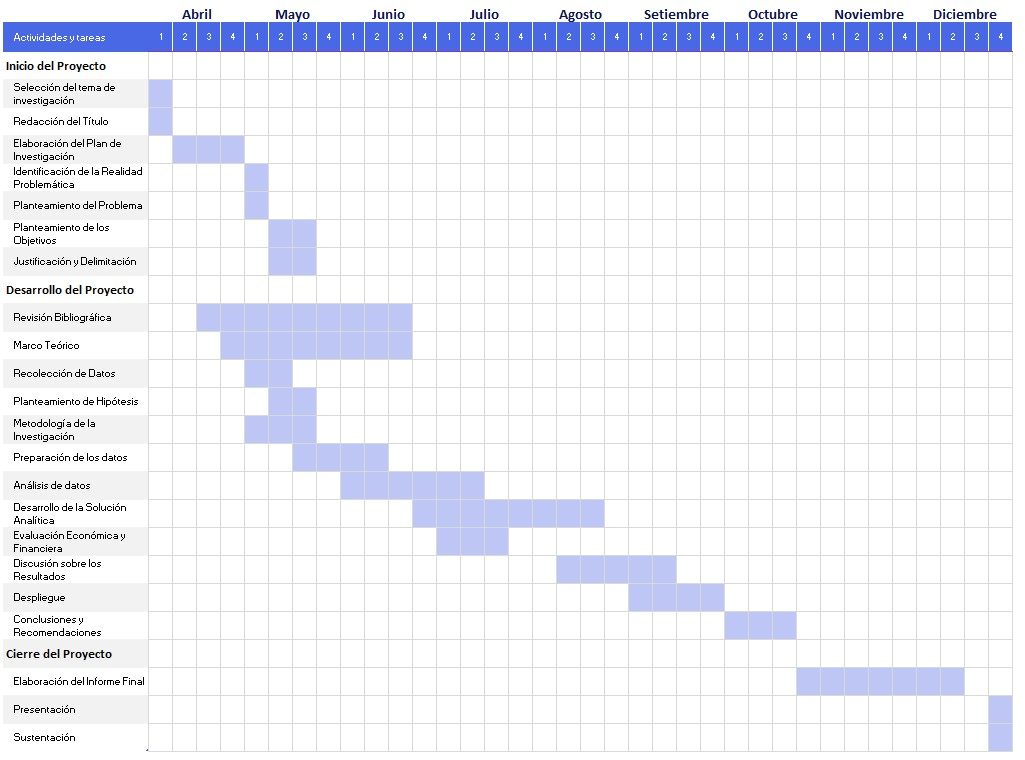
\includegraphics[width=1.35\textwidth]{3/figures/gantt.jpg}
			\caption[Cronograma de actividades]{Cronograma de actividades.\\
				Fuente: Elaboración propia.}
			\label{3:fig1}
		\end{center}
	\end{figure}
	
\end{landscape}

La Tabla 8 detalla los gastos relacionados con la investigación, incluyendo la compra de herramientas como una computadora portátil antes del inicio del proyecto, así como los costos asociados a actividades generales y al proceso de redacción y presentación pública de la tesis.

\begin{table}[h!]
	\caption{Presupuesto}
	\label{tab:presupuesto}
	\centering
	\small
	\begin{tabular}{p{6cm}rrr}
		\toprule
		\textbf{Concepto} & \textbf{Horas empleadas} & \textbf{Gasto (en soles)} & \textbf{Total} \\
		\midrule
		\multicolumn{4}{l}{\textbf{Activos físicos}} \\
		Portátil Lenovo Ideapad S340-15IIL Core i7 de 10ma GEN & -- & S/.5,700.00 & S/.5,700.00 \\
		\midrule
		\multicolumn{4}{l}{\textbf{Honorarios por el proceso de elaboración y defensa pública de la tesis}} \\
		Tasa de registro para el tema de investigación & -- & S/.800.00 & S/.800.00 \\
		Apartado del tema de tesis & -- & S/.2,700.00 & S/.2,700.00 \\
		Honorarios de defensa & -- & S/.1,500.00 & S/.1,500.00 \\
		\midrule
		\multicolumn{4}{l}{\textbf{Personal o equipo humano}} \\
		Progreso de tesis & 1000 & Inconmensurable & -- \\
		\midrule
		\multicolumn{4}{l}{\textbf{Gastos operativos}} \\
		Conexión a internet y servicio de electricidad (durante 8 meses) & 200 & S/.50.00 & S/.1000.00 \\
		\midrule
		\textbf{Python} & 50 & - & - \\
		\midrule
		\textbf{Suma total} & 1250 & -- & S/.11,700.00 \\
		\bottomrule
	\end{tabular}
	\begin{flushleft}
		\small Fuente: Elaboración propia.
	\end{flushleft}
\end{table}



%\chapter{Desarrollo del Experimento}
En este capítulo se detalla el proceso explicado en el capítulo anterior para cada actividad de la metodología aplicada, así como los entregables comprometidas.

\section{Comprensión del negocio}
\textbf{Actividad 1: Definir problemas, objetivos e hipótesis}
\\
El inicio de la implementación de la primera fase de la metodología CRISP-DM fue la identificación del problema general a partir del estudio de la realidad problemática abordada en los primeros capítulos. El objetivo, por lo tanto, busca resolver el problema y se encuentra alineado con el título de la investigación. Asimismo, la hipótesis resulta la proposición planteada para explicar el logro del objetivo. Los objetivos específicos del trabajo, que responde a cada problema específico, se definieron a partir de una lluvia de ideas en base a la asociación de objetivos específicos de los antecedentes con la actual investigación. Estos se explican en la siguiente actividad.

\textbf{Actividad 2: Desarrollar la literatura de la investigación}
\\
Se buscaron desde libros y artículos online para la comprensión teórica del financiamiento colectivo e Inteligencia Artificial, hasta papers publicados en conferencias, revistas internacionales y científicas, reportes técnicos y tesis de grado acerca de propuestas para resolver el problema estudiado en la investigación.

Para ello, como se describió en la sección 3.2, a través de búsqueda de palabras clave como \textit{crowdfunding}, \textit{Machine Learning}, \textit{Deep Learning}, \textit{prediction}, \textit{Kickstarter}, \textit{accuracy} y \textit{projects}, y el uso del buscador Google Académico, se encontraron estos papers publicados entre el 2013 y 2020.

A continuación, se realizó un resumen de cada antecedente en una hoja de cálculo de Excel con el fin de comparar sus objetivos y metodologías implementadas, como se puede observar el detalle en el Anexo \ref{anexo5}.

\textbf{Actividad 3: Definir metodología de la investigación}
\\
Luego de elaborar el detalle del anterior anexo, a excepción de la investigación del autor \cite{pr_fernandezblanco2020crowdfunding_empirical} que utilizó la metodología CRISP-DM, cada antecedente fue agrupado con otro similar de acuerdo a los pasos seguidos en su propia metodología. El resultado fue la Tabla \ref{2:table1} explicada en la sección 3.3.1.

\section{Comprensión de los datos}
\textbf{Actividad 1: Construir base de datos de Metainformación}
\\
El punto de partida para la construcción de los conjuntos de datos que se usaron más adelante en cada modelo de acuerdo a su modalidad fue la adquisición de bases de datos capturadas mensualmente desde finales del 2015 hasta 2019 por la página Web Robots (\url{https://webrobots.io/kickstarter-datasets/}), fundada por los ex corporativos de TI Tomás Vitulskis y Paulius Jonaitis, como se aprecia en la Figura \ref{4:fig1} \cite{ot_webrobots2019kickstarter}. Para el presente trabajo, se optó por descargar en archivos de valores separados por comas (.csv). De acuerdo sus creadores, se ejecutan robots en dos servidores en la nube encargados de recolectar en un determinado punto del día y una vez al mes información de las campañas que aparecen en Kickstarter.

\begin{figure}[!ht]
	\begin{center}
		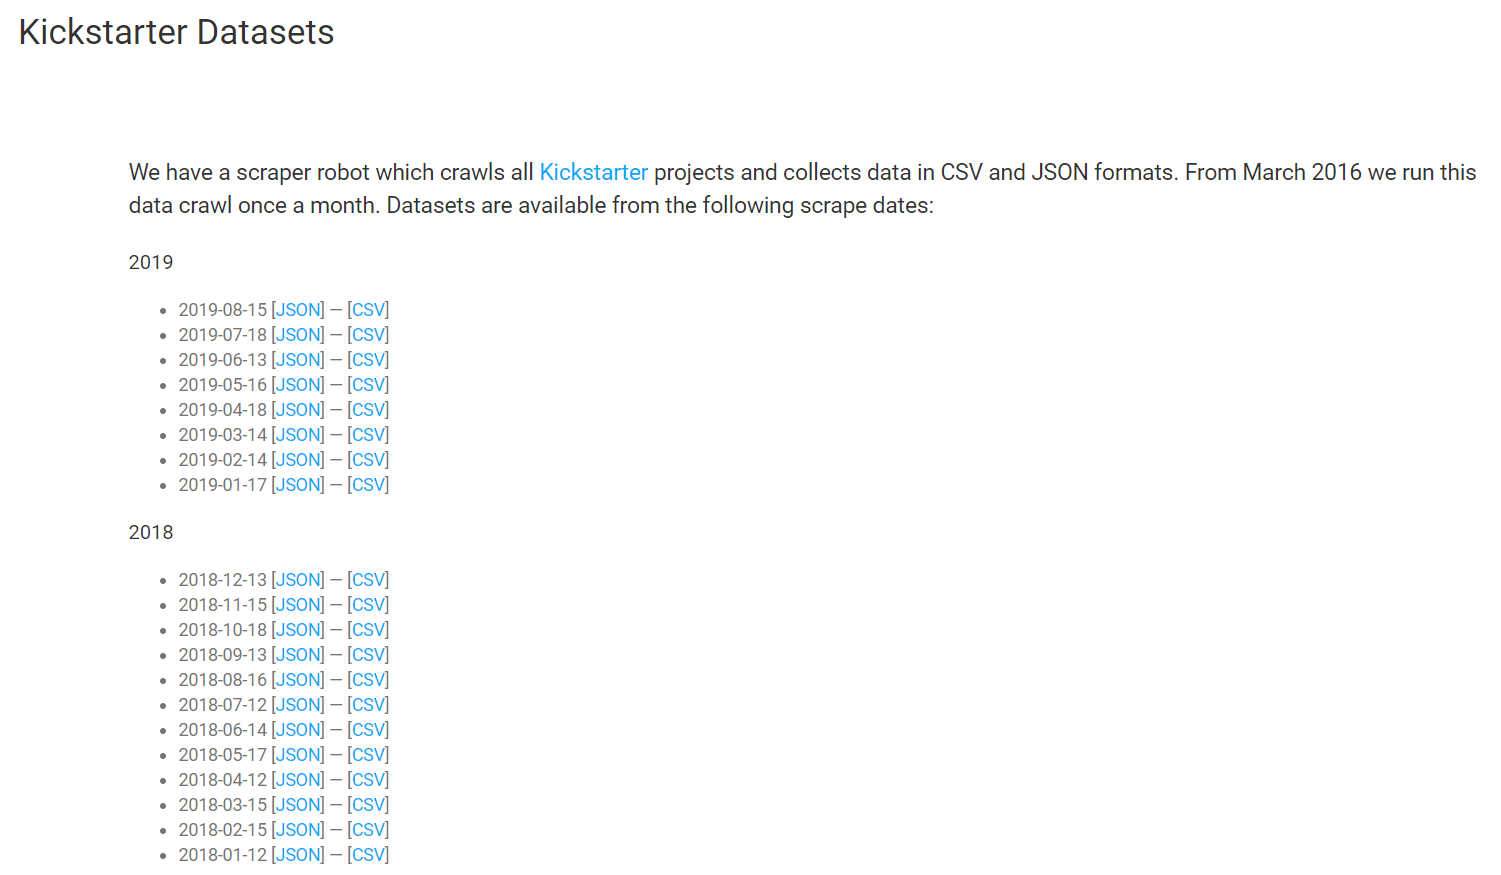
\includegraphics[width=1\textwidth]{4/figures/web_robots_2019.png}
		\caption[Vista del website Web Robots (visitado en agosto del 2019)]{Vista del website Web Robots (visitado en agosto del 2019).\\
		Fuente: Elaboración propia.}
		\label{4:fig1}
	\end{center}
\end{figure}

A continuación, los archivos descargados que se encontraban fraccionados en varios archivos .csv, donde luego de ser descomprimidos, fueron unidos por mes de captura y almacenados en carpetas independientes por mes, cuyo peso individual osciló entre 1 y 5 gigabytes (GB). Con el fin de ahorrar espacio en la computadora, las partes originales fueron eliminadas.

En la Figura \ref{4:fig2} se detalla el tamaño del conjunto de datos total al corte del periodo de captura de información Julio 2019, aproximadamente más de 212 mil proyectos de todas las categorías y 37 columnas de variables.

\begin{figure}[h]
	\begin{center}
		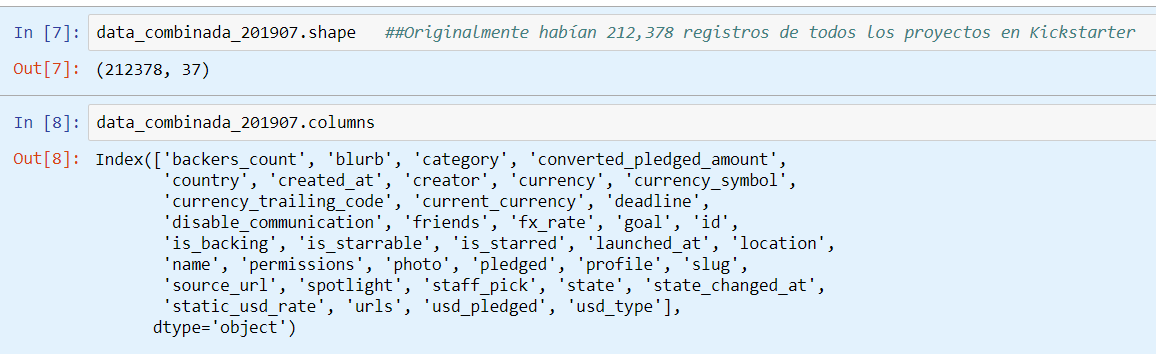
\includegraphics[width=1\textwidth]{4/figures/dataset_201907.png}
		\caption[Tamaño de conjunto de datos al corte de Julio 2019]{Tamaño de conjunto de datos al corte de Julio 2019.\\
			Fuente: Elaboración propia.}
		\label{4:fig2}
	\end{center}
\end{figure}

A cada conjunto de datos generado se filtraron los que pertenecen a la categoría \textit{\textbf{Technology}}. Al no contar con la información de la columna \textit{main\_category}, este proceso se logró utilizando la variable \textit{source\_url} seleccionando aquellos registros que contengan la cadena de caracteres “\textbf{https://www.kickstarter.com/discover/categories/technology}”.

Cuando se repitió este procedimiento con cada conjunto generado, se observó que la proporción de proyectos tecnológicos en Kickstarter representa el 10\% de la totalidad, aproximadamente más de 21 mil registros por mes. Esto se calculó al comparar el tamaño de cada conjunto generado con el total.

A continuación, se unieron los 45 archivos separados por coma (.csv) capturados mensualmente desde noviembre del 2015 hasta agosto del 2019. Se realizaron 2 uniones internamente ya que, a partir de marzo del 2018, algunas de las variables y valores presentan diferente estructura a la de sus predecesoras.

Luego, se realizó limpieza de datos para las variables \textit{category}, \textit{location}, \textit{photo} y \textit{urls}, y se transformaron las variables numéricas en milisegundos \textit{created\_at}, \textit{launched\_at} y \textit{deadline} a variables de fecha. Esto último permitió calcular la variable \textit{duration} para determinar la duración de la campaña (en días) de un proyecto calculando la diferencia entre la fecha de culminación (\textit{deadline}) y la fecha de lanzamiento (\textit{launched\_at}). Luego se excluyeron los proyectos en proceso de la variable \textit{state} para conservar los culminados, es decir, aquellos cuyo valor sea “successful” o “failed” ya que se analizarán solamente los proyectos que han sido exitosos o fracasados. Los proyectos cancelados o suspendidos no aparecieron. El último paso del flujo consistió en generar y exportar el archivo final en formato .csv. En la Figura \ref{4:fig4} se visualiza el conjunto final de Metainformación subido públicamente a la plataforma Kaggle. Cada variable se detalla en la Tabla \ref{4:table1}.

\begin{figure}[h]
	\begin{center}
		\includegraphics[width=0.93\textwidth]{4/figures/metadata_kaggle_preview.jpg}
		\caption[Visualización del archivo de metainformación subido a Kaggle]{Visualización del archivo de metainformación subido a Kaggle.\\
			Fuente: Elaboración propia.}
		\label{4:fig4}
	\end{center}
\end{figure}

\begin{table}[h!]
	\caption[Diccionario de datos del dataset final de Metainformación]{Diccionario de datos del dataset final de Metainformación.}
	\label{4:table1}
	\centering
	\small
	\begin{tabular}{ m{3cm}m{9.5cm}m{2.5cm} }
		\specialrule{.1em}{.05em}{.05em}
		\Centering{Variable}& \Centering{Detalle}& \Centering{Tipo de dato}\\
		\specialrule{.1em}{.05em}{.05em}
		id & Identificador del proyecto. & number \\
		%\hline
		backers\_count & Número de patrocinadores de la campaña del proyecto. & number \\
		%\hline
		name &	Nombre del proyecto. &	string \\
		%\hline
		blurb & Propaganda del proyecto. & string \\
		%\hline
		category & Categoría (dentro de categoría principal) del proyecto. & string \\
		%\hline
		photo & Dirección de enlace de la foto del proyecto. & string \\
		%\hline
		urls & Dirección de la página de la campaña del proyecto. & string \\
		%\hline
		city & Ciudad del creador del proyecto. & string \\
		%\hline
		country & Código de país del creador del proyecto. & string \\
		%\hline
		goal &	Monto de la meta de financiamiento del proyecto. &	float \\
		%\hline
		pledge\_amounts & Montos disponibles para patrocinar la campaña. & string \\
		%\hline
		pledged & Monto final patrocinado de la campaña. & float \\
		%\hline
		currency & Divisa del monto final patrocinado. & string \\
		%\hline
		usd\_pledged & Monto final patrocinado de la campaña (en USD). & float \\
		%\hline
		created\_at & Fecha de creación de la campaña. & date \\
		%\hline
		launched\_at & Fecha de lanzamiento de la campaña. & date \\
		%\hline
		deadline & Fecha de culminación de la campaña. & date \\
		%\hline
		duration &	Duración de la campaña (en días). &	number \\
		%\hline
		state & Estado de financiamiento del proyecto. & string \\
		\specialrule{.1em}{.05em}{.05em}
	\end{tabular}
	%\par	%%Salto de linea
	%\bigskip
	\begin{flushleft}	%%Alinear a la izquierda sin justificar
		\small Fuente: Elaboración propia.
	\end{flushleft}
\end{table}

\newpage
\textbf{Actividad 2: Construir base de datos de Descripción}
\\
La variable \textit{description} se obtuvo utilizando web scraping en cada proyecto gracias a la variable \textit{urls}. Para ello, se elaboró un algoritmo usando la librería BeautifulSoup que, mediante acceso y navegación al contenido de estas páginas a través de un agente falso, se dirigió a las descripciones de los proyectos identificando las etiquetas con clase llamada “\textbf{rte\_\_content js-full-description responsive-media}” y las almacenó en un vector vacío, uniendo previamente todos los párrafos y eliminando caracteres especiales, para posteriormente asignarle la id de su proyecto y guardarlo en un archivo de extensión .csv y exportarlo. En caso el algoritmo no encuentre esta clase dentro de las páginas (\textit{IndexError}), el vector almacena con el valor “null”.

\begin{figure}[!ht]
	\begin{center}
		\includegraphics[width=1\textwidth]{4/figures/description_scraping.jpg}
		\caption[Función para extraer textos de modalidad de descripción]{Función para extraer textos de modalidad de descripción.\\
			Fuente: Elaboración propia.}
		\label{4:fig5}
	\end{center}
\end{figure}

Debido a la gran cantidad de memoria y tiempo que iba a presentar este proceso, se determinó fraccionar los 27,251 proyectos en tres partes y repetir el mismo en cada uno de ellos. El tiempo aproximado de descarga de cada fracción fue de 6 horas.

Finalmente, las tres partes fueron unidas, se reemplazaron los valores nulos por espacios en blanco y se guardó como un nuevo archivo de valores separados por coma (.csv) en código Unicode UTF-8 para la lectura de caracteres no alfabéticos, como se observa en la Figura \ref{4:fig6}.

\begin{figure}[!ht]
	\begin{center}
		\includegraphics[width=0.95\textwidth]{4/figures/description_scraping_execution.jpg}
		\caption[Ejecución de la función de extracción de descripciones y almacenamiento]{Ejecución de la función de extracción de descripciones y almacenamiento.\\
			Fuente: Elaboración propia.}
		\label{4:fig6}
	\end{center}
\end{figure}

El archivo generado fue subido a la plataforma Kaggle de manera pública para que pueda ser descargada a través del API de la web, como se aprecia en la Figura \ref{4:fig7}.

\begin{figure}[!ht]
	\begin{center}
		\includegraphics[width=0.36\textwidth]{4/figures/description_kaggle_preview.jpg}
		\caption[Visualización del archivo de descripción subido a Kaggle]{Visualización del archivo de descripción subido a Kaggle.\\
			Fuente: Elaboración propia.}
		\label{4:fig7}
	\end{center}
\end{figure}

\textbf{Actividad 3: Construir base de datos de Comentarios}
\\
Al igual que la descripción, los comentarios se obtuvieron utilizando la variable \textit{urls} para web scraping, pero reemplazando caracteres que contengan desde “\textbf{?ref=}” en adelante, por “\textbf{/comments}” para redireccionarse a la sección de comentarios de cada proyecto. Para lograrlo, se codificó la función de la Figura \ref{4:fig8}.

\begin{figure}[!ht]
	\begin{center}
		\includegraphics[width=1\textwidth]{4/figures/comments_scraping.jpg}
		\caption[Función para extraer textos de modalidad de comentarios]{Función para extraer textos de modalidad de comentarios.\\
			Fuente: Elaboración propia.}
		\label{4:fig8}
	\end{center}
\end{figure}

Los comentarios, al ser dinámicos, no podían ser extraídos mediante la librería BeautifulSoup como en el caso de las descripciones, por lo que se utilizó la librería Selenium para extraerlos al iniciar una sesión desde Google Chrome. Una vez permitido el acceso al navegador, el algoritmo se redirecciona a la sección de comentarios del proyecto, espera un máximo de 30 segundos de carga de la página, busca el elemento Xpath “\textbf{//*[@id="react-project-comments"]/div/button}” para hacer clic en el botón “Load More” (Cargar más) hasta un máximo de 13 veces esperando 2 segundos entre cada clic, busca todos los comentarios bajo el nombre del elemento CSS “\textbf{div.w100p}”, elimina aquellos que pertenezcan al creador del proyecto identificados con etiqueta verde en el extremo superior derecho del recuadro del comentario con el nombre del elemento “\textbf{span.bg-ksr-green-700.white.px1.type-14.mr1}” (asignados con el valor de «Creator»), y almacena los restantes que pertenecen a los patrocinadores. En caso no encuentre ningún item de comentarios en la sección, se asignará un valor aleatorio no relacionado con proyectos. Luego de eliminar mensajes de la página acerca de comentarios ocultos o eliminados, el algoritmo culmina creando la lista de comentarios separados por autor y cerrando el web driver. Esta función fue ejecutada en 16 partes, asignando el id respectivo a los comentarios extraídos por cada proyecto en un archivo .csv, como se observa en la Figura \ref{4:fig9}.

\begin{figure}[!ht]
	\begin{center}
		\includegraphics[width=1\textwidth]{4/figures/comments_scraping_execution.jpg}
		\caption[Ejecución de la función de extracción de comentarios y almacenamiento]{Ejecución de la función de extracción de comentarios y almacenamiento.\\
			Fuente: Elaboración propia.}
		\label{4:fig9}
	\end{center}
\end{figure}

Para optimizar la descarga, se crearon 8 instancias en Google Cloud (Figura \ref{4:fig10}).

\begin{figure}[!ht]
	\begin{center}
		\includegraphics[width=0.95\textwidth]{4/figures/gc_instances_comments.jpg}
		\caption[Instancias lanzadas en paralelo para la extracción de comentarios]{Instancias lanzadas en paralelo para la extracción de comentarios.\\
			Fuente: Elaboración propia.}
		\label{4:fig10}
	\end{center}
\end{figure}

Cada instancia contenía dos copias del algoritmo, con la cantidad de proyectos fraccionada en 16 partes para que sean ejecutados en paralelo. Si bien el tiempo total de la consolidación de esta base de información duró aproximadamente un mes debido a percances de la conexión interna de las instancias y algunos problemas de ineficiencia de la primera versión del algoritmo, durante el transcurso dentro de este lapso de tiempo fueron solucionados hasta lograr optimizar el algoritmo de web scraping y tener el conjunto final de datos tomó menos de 48 horas. Este se encuentra disponible públicamente en Kaggle y se visualiza en la Figura \ref{4:fig11}.

\begin{figure}[!ht]
	\begin{center}
		\includegraphics[width=0.43\textwidth]{4/figures/comments_kaggle_preview.jpg}
		\caption[Visualización del archivo de comentarios subido a Kaggle]{Visualización del archivo de comentarios subido a Kaggle.\\
			Fuente: Elaboración propia.}
		\label{4:fig11}
	\end{center}
\end{figure}

\textbf{Actividad 4: Realizar análisis exploratorio y estadístico de variables considerados}
\\
En esta sección, se analizaron estadísticamente las variables de cada modalidad, tanto las distribuciones de sus datos para la metainformación y contenido textual, así como estadísticos para las variables cuantitativas de la metainformación, entre ellos el rango de sus valores, la media, la mediana, la moda, la desviación estándar y la varianza. En la variable dependiente estado de financiamiento, los 27,251 proyectos se distribuyen mediante el gráfico de pie de la Figura \ref{4:fig12}. Se observa que casi 20 mil proyectos entre 2009 y 2019 no llegaron a ser financiados, es decir, aproximadamente el 72\% del total fracasaron.

\begin{figure}[!ht]
	\begin{center}
		\includegraphics[width=0.60\textwidth]{4/figures/projects by state.png}
		\caption[Distribución de proyectos tecnológicos según su estado]{Distribución de proyectos tecnológicos según su estado.\\
			Fuente: Elaboración propia.}
		\label{4:fig12}
	\end{center}
\end{figure}

\newpage
De acuerdo a la distribución por año de la Figura \ref{4:fig13}, 2015 fue el periodo en donde se registraron más campañas de proyectos tecnológicos en la plataforma.

\begin{figure}[!ht]
	\begin{center}
		\includegraphics[width=0.77\textwidth]{4/figures/projects state by year.png}
		\caption[Evolución de cantidad de proyectos tecnológicos por año]{Evolución de cantidad de proyectos tecnológicos por año.\\
			Fuente: Elaboración propia.}
		\label{4:fig13}
	\end{center}
\end{figure}

El anterior gráfico abierto por estado de financiamiento, como se representa en la Figura \ref{4:fig14}, muestra que el 2015 resultó ser el año más disparejo, donde el 78\% fueron fracasados.

\begin{figure}[!ht]
	\begin{center}
		\includegraphics[width=0.77\textwidth]{4/figures/projects state evolution by year.png}
		\caption[Evolución de proyectos tecnológicos, por su estado y año]{Evolución de proyectos tecnológicos, por su estado y año.\\
			Fuente: Elaboración propia.}
		\label{4:fig14}
	\end{center}
\end{figure}

Por el lado de Metainformación, de las 19 variables de la Tabla \ref{4:table1}, se consideraron como potenciales variables independientes a 3 categóricas, 5 numéricas y 1 lista compuesta por números (\textit{pledge\_amounts}). La distribución del primer grupo se ilustra en la Figura \ref{4:fig15}.

\begin{figure}[!ht]
	\centering
	\small
	\begin{subfigure}{.35\textwidth}
		\centering
		\includegraphics[width=1.13\linewidth]{4/figures/country_distribution.png}
		\caption{país}
	\end{subfigure}%
	\begin{subfigure}{.36\textwidth}
		\centering
		\includegraphics[width=1.13\linewidth]{4/figures/currency_distribution.png}
		\caption{divisa}
	\end{subfigure}%
	\begin{subfigure}{.35\textwidth}
		\centering
		\includegraphics[width=1.15\linewidth]{4/figures/category_distribution.png}
		\caption{categoría}
	\end{subfigure}
	\caption[Distribución de las variables categóricas de Metainformación]{Distribución de las variables categóricas de Metainformación.\\
		Fuente: Elaboración propia.}
	\label{4:fig15}
\end{figure}

De las 3 variables categóricas (\textit{country}, \textit{currency} y \textit{category}), se observa que más de la mitad de creadores proyectos provienen de los Estados Unidos (64\%) e invierten en dólares. A ellos los acompañan personas de Gran Bretaña (9\%), que invierten en libras esterlinas, y de Canadá (6\%), que invierten en dólares canadienses. El 21\% restante provienen de otros países, donde el 12\% de ellos invierten en euros. Por el lado de las categorías, las más resaltantes son Apps, Web, Hardware, Software y Gadgets.

Para las potenciales variables numéricas de Metainformación (\textit{backers\_count}, \textit{goal}, \textit{pledged}, \textit{usd\_pledged} y \textit{duration}), se calcularon sus datos estadísticos de rango de valores, media, mediana, desviación estándar y varianza, con ayuda de diagramas de caja y bigote que se muestran a continuación:

\begin{itemize}
	\item Número de patrocinadores de la campaña (\textit{backers\_count}):
	\begin{itemize}
		\item Rango de valores: [0; 105,857]
		\item Media: 208.710469340575
		\item Mediana: 9.487
		\item Desviación estándar: 1,179.68237749203
		\item Varianza: 1,391,650.51176525
		\begin{figure}[!ht]
			\begin{center}
				\includegraphics[width=0.80\textwidth]{4/figures/caja_bigote_backers.png}
				\caption[Diagrama de caja y bigote de patrocinadores]{Diagrama de caja y bigote de patrocinadores.\\
					Fuente: Elaboración propia.}
				\label{4:fig16}
			\end{center}
		\end{figure}
	\end{itemize}
	\item Monto meta de la campaña (\textit{goal}):
	\begin{itemize}
		\item Rango de valores: [1; 100,000,000]
		\item Media: 91,263.9666162825
		\item Mediana: 15,762.614
		\item Desviación estándar: 1,259,282.1587922
		\item Varianza: 1,585,791,555,452.35
		\begin{figure}[!ht]
			\begin{center}
				\includegraphics[width=0.80\textwidth]{4/figures/caja_bigote_goal.png}
				\caption[Diagrama de caja y bigote de meta]{Diagrama de caja y bigote de meta.\\
					Fuente: Elaboración propia.}
				\label{4:fig17}
			\end{center}
		\end{figure}
	\end{itemize}
	\item Monto patrocinado al final de la campaña (\textit{pledged}):
	\begin{itemize}
		\item Rango de valores: [0; 17,406,300]
		\item Media: 34,668.5134710787
		\item Mediana: 1,382.933
		\item Desviación estándar: 226,763.900313481
		\item Varianza: 51,421,866,485.3822
		\begin{figure}[!ht]
			\begin{center}
				\includegraphics[width=0.80\textwidth]{4/figures/caja_bigote_pledged.png}
				\caption[Diagrama de caja y bigote de monto patrocinado]{Diagrama de caja y bigote de monto patrocinado.\\
					Fuente: Elaboración propia.}
				\label{4:fig18}
			\end{center}
		\end{figure}
	\end{itemize}
	\item Duración de la campaña (\textit{duration}).
	\begin{itemize}
		\item Rango de valores: [1; 92]
		\item Media: 35.4654141132436
		\item Mediana: 30
		\item Desviación estándar: 11.84570862999998
		\item Varianza: 140.320812946853
		\begin{figure}[!ht]
			\begin{center}
				\includegraphics[width=0.80\textwidth]{4/figures/caja_bigote_duration.png}
				\caption[Diagrama de caja y bigote de duración]{Diagrama de caja y bigote de duración.\\
					Fuente: Elaboración propia.}
				\label{4:fig19}
			\end{center}
		\end{figure}
	\end{itemize}
\end{itemize}

\newpage
Posterior a este entendimiento de datos, se elaboró una matriz de correlaciones (Figura \ref{4:fig20}) para encontrar correlaciones entre ellas y determinar la existencia de alguna variable redundante y descartarla para no afectar el rendimiento del modelo.

\begin{figure}[!ht]
	\begin{center}
		\includegraphics[width=0.90\textwidth]{4/figures/metadata correlation.png}
		\caption[Matriz de correlaciones entre variables independientes]{Matriz de correlaciones entre variables independientes.\\
			Fuente: Elaboración propia.}
		\label{4:fig20}
	\end{center}
\end{figure}

Como se puede apreciar en la figura anterior, la variable \textit{usd\_pledged} está altamente correlacionada con las variables \textit{backers\_count} y \textit{pledged} (ambas con un aproximado de 70\%). Esto quiere decir que dicha variable no es significativa porque explicaría de manera muy similar a las otras dos.

\newpage
Asimismo, si se observan los registros desde una matriz que contiene, además de gráficos de dispersión de las correlaciones, histogramas de las variables independientes como en la Figura \ref{4:fig21}, se confirma y concluye no utilizar las observaciones comentadas.

\begin{figure}[!ht]
	\begin{center}
		\includegraphics[width=1.00\textwidth]{4/figures/metadata cor-plot2.png}
		\caption[Gráfico de dispersión de correlaciones entre variables independientes]{Gráfico de dispersión de correlaciones entre variables independientes.\\
			Fuente: Elaboración propia.}
		\label{4:fig21}
	\end{center}
\end{figure}

La variable \textit{duration} es la única que sigue una distribución normal debido a la forma de campana de su silueta. Asimismo, los registros de proyectos exitosos y fracasados para las otras 4 variables se encuentran mezcladas en los mismos grupos al cruzarse entre ellas. También se visualizan observaciones en los extremos de cada gráfico, tal y como se detalló en sus valores estadísticos individuales.

\newpage
Por el lado de Descripción, solo 640 proyectos (2\% del total) no presentaron descripciones por razones externas durante el proceso de extracción de datos. De ellos, 512 (80\% de proyectos sin descripciones) fracasaron en ser financiados. Por el lado de proyectos con descripciones, casi el 30\% fueron exitosos como se grafica en la Figura \ref{4:fig22}.

\begin{figure}[!ht]
	\begin{center}
		\includegraphics[width=0.75\textwidth]{4/figures/projects description by state.png}
		\caption[Distribución de proyectos por presencia de descripciones y estado final]{Distribución de proyectos por presencia de descripciones y estado final.\\
			Fuente: Elaboración propia.}
		\label{4:fig22}
	\end{center}
\end{figure}

Asimismo, el registro con descripción de mayor longitud presentó 5,152 palabras y, a nivel total de proyectos, el vocabulario fue de 165,683 palabras.

\begin{figure}[!ht]
	\begin{center}
		\includegraphics[width=0.64\textwidth]{4/figures/description_wordcloud_original_data.png}
		\caption[Nube de palabras de descripciones]{Nube de palabras de descripciones.\\
			Fuente: Elaboración propia.}
		\label{4:fig23}
	\end{center}
\end{figure}

En la nube de palabras de la anterior Figura \ref{4:fig23}, los términos más frecuentes en ellas se relacionan con las funcionalidades del producto (\textit{system}, \textit{app}, \textit{need}, \textit{help}, \textit{product}, etc).

Por el lado de Comentarios, al analizar los proyectos exitosos y fracasados por la presencia de comentarios (Figura \ref{4:fig24}), se observa que el 60\% de proyectos con comentarios (4,626 registros) fueron exitosos, mientras que el 84\% de los proyectos sin comentarios fracasaron.

\begin{figure}[!ht]
	\begin{center}
		\includegraphics[width=0.80\textwidth]{4/figures/projects comment by state.png}
		\caption[Distribución de proyectos por presencia de comentarios y estado final]{Distribución de proyectos por presencia de comentarios y estado final.\\
			Fuente: Elaboración propia.}
		\label{4:fig24}
	\end{center}
\end{figure}

Esto señala que es más probable que un proyecto sin recibir comentarios tiende a fracasar por la diferencia notable entre ambas categorías (68\%). Por el contrario, para el caso de aquellos que presentan comentarios, no se puede formular una hipótesis sobre su comportamiento ya que la diferencia de proporciones no es muy alta (20\%) en comparación con el grupo sin comentarios. Por ello, para conocer un poco más a este último grupo, se analizó el impacto de las cantidades de comentarios independientes realizados por patrocinadores exclusivamente en el resultado final de la meta de financiamiento.

\newpage
De aquellos proyectos con comentarios, el 96\% que fueron financiados exitosamente recogieron más de 475 mil comentarios, como se aprecia en la Figura \ref{4:fig25}.

\begin{figure}[!ht]
	\begin{center}
		\includegraphics[width=0.44\textwidth]{4/figures/total comments by projects state.png}
		\caption[Distribución de comentarios en proyectos exitosos y fracasados]{Distribución de comentarios en proyectos exitosos y fracasados.\\
			Fuente: Elaboración propia.}
		\label{4:fig25}
	\end{center}
\end{figure}

Respecto al contenido, en la Figura \ref{4:fig26} se ilustra la nube de palabras más frecuentes, respectivamente, luego de quitar URLs, emoticonos y términos en idioma distinto al inglés.

\begin{figure}[htbp]
	\begin{center}
		\includegraphics[width=0.68\textwidth]{4/figures/comments_wordcloud_wordunit.png}
		\caption[Nube de palabras de comentarios más frecuentes]{Nube de palabras de comentarios más frecuentes.\\
			Fuente: Elaboración propia.}
		\label{4:fig26}
	\end{center}
\end{figure}

De esta imagen, se observa que las palabras más frecuentes en los comentarios (tamaño de fuente más grande) se relacionan con términos clave respecto a la campaña (\textit{update}, \textit{project}, \textit{backer}, \textit{product} y \textit{Kickstarter}) y palabras relacionadas a su interacción con el público (\textit{thank}, \textit{will}, \textit{received}, \textit{time}, \textit{money}). Algunos de estos términos, tanto en su forma raíz como en conjugaciones, suelen aparecer solitarias o acompañados de otros para formar frases recurrentes.

\section{Preparación de los datos}
\textbf{Actividad 1: Pre-procesar base de datos de Metainformación}
\\
De acuerdo a los autores \cite{pr_chen2013kickpredict}, \cite{pr_chen2015predcrowd} y \cite{pr_jin2019dayssuccess}, a las 5 potenciales variables numéricas se adicionaron 7 variables basadas en el mecanismo financiero (mediana (\textit{pledges\_median}), promedio (\textit{pledges\_mean}), valor máximo (\textit{pledges\_max}), valor mínimo (\textit{pledges\_min}), variación estándar (\textit{pledges\_std}) y cantidad de montos disponibles para contribuir (\textit{pledges\_num})) y efecto progresión (porcentaje de financiamiento o completitud (\textit{completeness}) del monto prometido). Esta última se calcula dividiendo el monto alcanzado en el tiempo t, sobre la meta de la campaña, multiplicado por 100\%. La nueva matriz de correlación se observa en la Figura \ref{4:fig27}.

\begin{figure}[!ht]
	\begin{center}
		\includegraphics[width=1.00\textwidth]{4/figures/metadata correlation v2.png}
		\caption[Matriz de correlaciones entre variables independientes considerando adicionales]{Matriz de correlaciones entre variables independientes considerando adicionales.\\
			Fuente: Elaboración propia.}
		\label{4:fig27}
	\end{center}
\end{figure}

\newpage
Para la selección de variables, se consideró a aquellas con correlación clasificada como insignificante, es decir, menor o igual a 0.30 \parencite{tec_mukaka2012correlation}. Las únicas que cumplen son \textit{goal}, \textit{pledges\_num}, \textit{completeness} y \textit{duration}. Sin embargo, algunas de las restantes pueden ser consideradas condicionándose a excluir otras. En la Tabla \ref{4:table2} se listan las 8 combinatorias posibles de variables que se pueden formar.

\begin{table}[h!]
	\caption[Potenciales combinatorias de variables de metainformación]{Potenciales combinatorias de variables de metainformación.}
	\label{4:table2}
	\centering
	\small
	\begin{tabular}{ m{3.5cm}m{3.5cm}m{3.5cm}m{3.5cm}  }
		\specialrule{.1em}{.05em}{.05em}
		%\rowcolor{bluejean}
		\Centering{Combinación 1}& \Centering{Combinación 2}& \Centering{Combinación 3}& \Centering{Combinación 4}
		\\
		\specialrule{.1em}{.05em}{.05em}
		goal & goal & goal & goal \\
		\hline
		completeness & completeness & completeness & completeness
		\\
		\hline
		duration & duration & duration & duration
		\\
		\hline
		pledges\_num & pledges\_num & pledges\_num & pledges\_num
		\\
		\hline
		backers\_count & backers\_count & backers\_count & backers\_count \\
		\hline
		pledges\_median & pledges\_mean & pledges\_min & pledges\_max \\
		\hline
		&  & pledges\_std &  \\
		\specialrule{.1em}{.05em}{.05em}
		\Centering{Combinación 5}& \Centering{Combinación 6}&
		\Centering{Combinación 7}& \Centering{Combinación 8}
		\\
		\specialrule{.1em}{.05em}{.05em}
		goal & goal & goal & goal
		\\
		\hline
		completeness & completeness & completeness & completeness
		\\
		\hline
		duration & duration & duration & duration
		\\
		\hline
		pledges\_num & pledges\_num & pledges\_num & pledges\_num
		\\
		\hline
		pledged & pledged & pledged & pledged \\
		\hline
		pledges\_median & pledges\_mean & pledges\_min & pledges\_max \\
		\hline
		&  & pledges\_std &  \\
		\specialrule{.1em}{.05em}{.05em}
	\end{tabular}
	%\par	%%Salto de linea
	%\bigskip
	\begin{flushleft}	%%Alinear a la izquierda sin justificar
		\small Fuente: Elaboración propia.
	\end{flushleft}
\end{table}

Una vez generadas las variables independientes (X) y dependiente (Y), el conjunto de datos es separado en subconjuntos de entrenamiento y prueba, con proporciones de 80\% y 20\% respectivamente \citep{pr_yuan2016textanalytics,pr_yu2018deeplearning,pr_chen2019keywords_crowdfunding,pr_mitra2014phrases,pr_sawhney2016usingLT} y se fija un valor de aleatoriedad. Dentro de los parámetros de separación, se establece el argumento de estratificación según la variable Y, es decir, cada subconjunto mantendrá la distribución 72\% exitosos y 28\% fracasados.

\begin{figure}[!ht]
	\begin{center}
		\includegraphics[width=1.00\textwidth]{4/figures/train_test_split.jpg}
		\caption[Función para dividir base de datos en subconjuntos de entrenamiento y prueba]{Función para dividir base de datos en subconjuntos de entrenamiento y prueba.\\
			Fuente: Elaboración propia.}
		\label{4:fig28}
	\end{center}
\end{figure}

Luego, utilizando el escalador Mínimo Máximo (\textit{Min-Max scaler}) de la librería Scikit-learn, se normalizaron las variables independientes a un nuevo rango conformando valores entre 0 y 1. La función creada para este proceso se muestra en la Figura \ref{4:fig29}.

\begin{figure}[!ht]
	\begin{center}
		\includegraphics[width=0.95\textwidth]{4/figures/metadata_scaler_function.jpg}
		\caption[Función para normalizar variables]{Función para normalizar variables.\\
			Fuente: Elaboración propia.}
		\vspace{-0.5cm}
		\label{4:fig29}
	\end{center}
\end{figure}

Para calcular los nuevos valores normalizados usando el anterior escalador, se sigue la siguiente fórmula \citep{tec_minmaxscaler,tec_scikitlearn,tec_datascaling}:

\begin{equation}\label{eq:minmaxscaler}
\phantomsection
x_{escalado}=\frac{x-x_{min}}{x_{max}-x_{min}}
\end{equation}
\myequations{Fórmula del escalador Mínimo Máximo}

Donde $x$ representa el valor original de un dato, $x_{min}$ el valor mínimo existente para dicha variable y $x_{max}$, el valor máximo.

Por ejemplo, tomando como referencia las estadísticas de la variable \textit{duration} en la Figura \ref{4:fig19}, se desea transformar una duración de 30 días dentro del rango [0; 1]. Para aplicar la fórmula, los valores serían $x=30$, $x_{min}=1$ y $x_{max}=92$. Entonces, el nuevo resultado sería $x_{escalado}=\frac{30-1}{92-1}=0.32$.

\vspace{0.5cm}
\textbf{Actividad 2: Pre-procesar base de datos de Descripción}
\\
Se realizó la limpieza de texto basándose en los trabajos de los autores \cite{pr_mitra2014phrases}, \cite{pr_yuan2016textanalytics} y \cite{pr_chen2019keywords_crowdfunding} y además, se agregaron pasos de lematización y supresión de palabras de parada siguiendo el proceso dictado en el curso de Procesamiento de Lenguaje Natural en la Escuela Superior de Economía de la Universidad Nacional de Investigación, Rusia \parencite{tec_zimovnov2018text_preprocessing}. Antes de ejecutarse el proceso, los registros sin descripciones (\textit{NaN}) fueron convertidos en cadena (\textit{string}) para evitar problemas de procesamiento de texto. Se remueven las contracciones, caracteres especiales, enlaces externos y contenidos en otros idiomas. Este resultado fue separado en palabras o tókens para eliminar palabras de parada en inglés, lematizar las restantes y finalmente juntarlas en una lista por su proyecto.

Cada iteración se pudo lograr gracias a elementos de la biblioteca para procesamiento de lenguaje natural Natural Language Toolkit (NLTK), como por ejemplo \textit{word\_tokenize}, \textit{stopwords} y \textit{WordNetLemmatizer}. La descripción de mayor longitud pasó a presentar 3,671 palabras y a nivel general de proyectos, el nuevo vocabulario tuvo 165,526 palabras.

Las nubes de palabras reflejan las palabras más frecuente dentro de un conjunto de datos. La Figura \ref{4:fig30} representa aquellas palabras que más aparecen en las descripciones.

\begin{figure}[!ht]
	\begin{center}
		\includegraphics[width=0.65\textwidth]{4/figures/description_wordcloud.png}
		\caption[Nube de palabras de descripciones posterior a la limpieza de texto]{Nube de palabras de descripciones posterior a la limpieza de texto.\\
			Fuente: Elaboración propia.}
		\label{4:fig30}
	\end{center}
\end{figure}

Luego de la limpieza de textos, la variable independiente \textit{description}, como en el caso de Metainformación, fue dividida en subconjuntos de 80\% para entrenamiento y 20\% para prueba, estratificados según la distribución de la variable \textit{state}. A continuación, en la Figura \ref{4:fig31} se ejecuta el proceso para representar las palabras de las descripciones en vectores.

\begin{figure}[!ht]
	\begin{center}
		\includegraphics[width=0.95\textwidth]{4/figures/description_word_representation.jpg}
		\caption[Proceso de representación de palabras en vectores codificados]{Proceso de representación de palabras en vectores codificados.\\
			Fuente: Elaboración propia.}
		\label{4:fig31}
	\end{center}
\end{figure}

De acuerdo al algoritmo de la figura anterior, se usó la función \textit{Tokenizer} de la librería \textbf{tensorflow.keras.preprocessing.text}, para separar las palabras únicas o \textit{tokens} de una línea de texto asignada. En caso se encuentre un término no identificado dentro del diccionario a entrenar, se asignará a dicho token el valor de \textit{$<$OOV$>$}. Esta función se aplicó al subconjunto de entrenamiento para elaborar un diccionario a partir de sus tokens. Luego, se creó una función para determinar la mayor longitud de palabras de las descripciones del dataset. Esta cantidad representó 3,671 términos. A continuación, se desarrolló una función para crear una secuencia de las palabras codificadas, homologar hasta la máxima longitud de descripciones y rellenar con ceros a la derecha (parámetro \textit{padding=`post'}) en caso un vector no alcance esta longitud. Se aplicó este proceso a los subconjuntos originales de entrenamiento y prueba.

Una vez obtenido el vocabulario de palabras únicas y asignado el tamaño de cada arreglo (en este caso, se asignó el de la descripción de mayor longitud), se procedió a elaborar la matriz de características usando incrustaciones de GloVe como se observa en la Figura \ref{4:fig32}. Para la presente investigación, se seleccionó la opción Wikipedia 2014 + Gigaword 5, con una matriz de 100 columnas, donde cada una contendrá las incrustaciones de palabras GloVe para las palabras del corpus, cuyos índices se corresponderán con cada número de fila \parencite{tec_malik2019pythonnlp}.

\begin{figure}[!ht]
	\begin{center}
		\includegraphics[width=0.75\textwidth]{4/figures/description_embedding_matrix.jpg}
		\caption[Proceso de creación de matriz de incrustaciones de palabras]{Proceso de creación de matriz de incrustaciones de palabras.\\
			Fuente: Elaboración propia.}
		\label{4:fig32}
	\end{center}
\end{figure}

En la figura anterior, luego de abrirse el archivo GloVe, se completa un diccionario creado con los registros extraídos del algoritmo GloVe. Luego de terminarse este proceso y cerrarse el archivo, se crea la matriz de incrustación de palabras que será utilizada más adelante en la capa de incrustación del modelo predictivo.

\textbf{Actividad 3: Pre-procesar base de datos de Comentarios}
\\
La base de datos de comentarios está conformada a nivel de 1 proyecto con una lista de comentarios separados en sublistas. De los 7,750 proyectos con comentarios (4,626 exitosos), se removieron aquellos que presentaron términos en idioma distinto al inglés, URLs, emoticonos, emojis, números y caracteres especiales, quedando 7,658 registros (4,574 exitosos).

Debido a la gran cantidad de registros carecientes de comentarios, se propuso rellenarlos con un término aleatorio no relacionado con las temáticas principales: \textit{kuwagatabaizan}. Posteriormente, se repitió el mismo ejercicio para las descripciones. Sin considerar este nuevo término, la nube de palabras se representa en la Figura \ref{4:fig33}.

\begin{figure}[!ht]
	\begin{center}
		\includegraphics[width=0.63\textwidth]{4/figures/comments_wordcloud_processed.png}
		\caption[Nube de palabras de comentarios posterior a la limpieza de texto]{Nube de palabras de comentarios posterior a la limpieza de texto.\\
			Fuente: Elaboración propia.}
		\label{4:fig33}
	\end{center}
\end{figure}

Al igual que el caso de Descripción, se siguieron los procesos de la Figura \ref{4:fig31} para obtener la representación de palabras en vectores codificados y la Figura \ref{4:fig32} para crear la matriz de incrustación de palabras que se usarán en la capa de incrustaciones, con la diferencia en que el tamaño de la secuencia de palabras codificadas no será la máxima longitud de comentarios ya que estos, inicialmente separados por autor, al ser concatenados en un solo registro por proyecto, ampliaron su longitud exponencialmente. La máxima longitud de todos los registros fue de 30,072 palabras; por ello, se limitó el tamaño de secuencias a 5,000 términos.
%\chapter{Análisis y Discusión de Resultados}
En este capítulo, se continuaron las 3 últimas fases de la metodología seleccionada.

\section{Modelamiento}
Antes de crear los modelos correspondientes, y después de definir los valores de entrada y parámetros (las subsecciones que se detallarán a continuación), se asigna una semilla inicial con un valor fijado por el usuario con el fin de evitar resultados aleatorios para futuras iteraciones. Se establece, además, una ruta local en donde se almacena cada punto de control basado en la mejora de la pérdida del subconjunto de validación con respecto a su iteración anterior. En caso de un estancamiento de esta última durante 10 épocas, es decir, si el valor de la pérdida no decrementa, el modelo dejará de entrenar. A esta regla se le añade la reducción de la tasa de aprendizaje luego de 5 épocas en caso el valor de la exactitud del subconjunto de validación no refleje un incremento. El objetivo de estas condiciones es evitar el sobreajuste en los modelos durante el entrenamiento.

Por último, es importante asignar un peso distinto para cada una de las dos clases de la variable dependiente \textit{state}. Con el fin de evitar un mal entrenamiento, los pesos de ambas clases se balancean y se almacenan en un diccionario con su etiqueta correspondiente.

\textbf{Actividad 1: Desarrollar modelo predictivo de Metainformación}
\\
Se diseñó el modelo de descripciones basada en un Perceptrón Multicapa (MLP por sus siglas en inglés) bajo la arquitectura de la Figura \ref{4:fig34} y teniendo como referencia a los autores \citeauthor{pr_yu2018deeplearning}. Se asignaron 100 épocas y el número de lotes fue 32.

\begin{figure}[!ht]
	\begin{center}
		\includegraphics[width=0.43\textwidth]{4/figures/model_mlp_metadata.png}
		\caption[Arquitectura de modelo MLP para la metadata]{Arquitectura de modelo MLP para la metadata.\\
			Fuente: Elaboración propia.}
		\vspace{-0.5cm}
		\label{4:fig34}
	\end{center}
\end{figure}

La arquitectura comienza con la capa de entrada alimentadas por las 6 variables consideradas, que representan la cantidad de neuronas, tanto de entrada como de salida.

Si bien no existe alguna regla general para definir el número de capas óptimas, así como los hiperparámetros que se deben configurar en ellas, se puede utilizar como referencia algunas metodologías como las Reglas del Pulgar según \cite{tec_ranjan2019thumbrules}.

De acuerdo a una de ellas, el número de capas ocultas comienza con 2 sin contar la última. La primera capa densa continúa a la capa de entrada, mientras que la segunda aparece después de la primera capa de desactivación.

Otro punto considerado fue el número de nodos o neuronas de las capas intermedias. Estas deben seguir una progresión geométrica de 2, donde la primera capa debe ser la mitad del número de variables en la capa de entrada. Dado que la mitad de 6 es un valor que no cumple, un número potencial puede ser 4.

El autor también menciona tener en consideración utilizar la función de activación \textit{\textbf{relu}} para las capas intermedias, una tasa de abandono de por lo menos 0.5 para las capas de desactivación, tamaño de salida de 1 neurona y función de activación \textit{\textbf{sigmoide}} por tratarse de un problema de clasificación binaria, utilizar el optimizador \textit{\textbf{adam}}, comenzar con 20 épocas en adelante de acuerdo al progreso de los resultados y fijar un tamaño de lote bajo progresión geométrica de 2; además de otros requerimientos previamente establecidos como la ponderación de clases para la variable dependiente en caso de datos desbalanceados y escalado de datos antes del entrenamiento.

Estas opciones fueron probadas en el modelo y evaluadas con las métricas correspondientes. Sin embargo, al calibrar el modelo y comparar distintos resultados, se obtuvo que la mejor cantidad de neuronas para la primera capa densa era de 32. De este modo, la siguiente capa intermedia se le asignó la mitad (16). La función de activación \textit{\textbf{tanh}} para la segunda capa oculta presentó mejores resultados, así como tasas de abandono entre 0.25 y 0.3 para las capas de desactivación. El criterio para elegir esta función se explica en el modelo de descripción, en el cual también fue aplicado. Por último, además de \textit{adam}, se realizó experimentos con otros optimizadores como por ejemplo \textit{RMSprop} siendo este el resultado más cercano. Al final, \textit{adam} fue escogido pero con una tasa de aprendizaje baja como 0.005 debido a que el modelo tendía a aprender muy rápido durante el transcurso de las épocas. Al ratio de decaimiento se le asignó, entonces, el valor de 0.00005 y para evaluar el modelo se usó la exactitud.

El resumen de la explicación anterior, desde la configuración de parámetros para entrenar hasta los elementos presentes en cada capa, se encuentra en el Anexo \ref{anexo6}.

%\newpage
\textbf{Actividad 2: Desarrollar modelo predictivo de Descripción}
\\
Se diseñó el modelo de descripciones basada en una Red Neuronal Convolucional unidimensional (Conv1D) bajo la arquitectura de la Figura \ref{4:fig35}, así como de referencia un trabajo de análisis de sentimientos de películas \parencite{tec_malik2019pythonnlp}. Se asignaron 100 épocas para entrenar y número de lotes de 128.

\begin{figure}[!ht]
	\begin{center}
		\includegraphics[width=0.63\textwidth]{4/figures/model_cnn_description.png}
		\caption[Arquitectura de modelo CNN para las descripciones]{Arquitectura de modelo CNN para las descripciones.\\
			Fuente: Elaboración propia.}
		\vspace{-0.5cm}
		\label{4:fig35}
	\end{center}
\end{figure}

Esta red se compone de una capa de incrustación de palabras o \textit{Embedding} alimentada por los datos de entrada en la primera capa \textit{InputLayer} de dimensión de 3,671 vectores de palabras (la mayor longitud de palabras de todas las descripciones), la cual genera como salida una matriz de 3,671 por 100 (número de columnas de incrustaciones de GloVe). Para esta capa se entrenarán 14,827,000 parámetros como resultado del producto de las 100 columnas mencionadas y 148,270 como el tamaño del vocabulario entrenado.

La siguiente capa es la Convolución en 1 dimensión o \textit{Conv1D} (usado frecuentemente para extraer características de datos de textos por ser unidimensionales) que, con 128 características, 5 de tamaño de kernel y función de activación \textit{\textbf{relu}}, generó una salida de 3,667 por 128; así como 64,128 parámetros entrenables.

A continuación, le sigue la capa de reducción \textit{GlobalMaxPooling}. Al igual que en la convolución, esta también fue unidimensional y se caracteriza por realizar agrupamiento global basado en el valor máximo de los bloques seleccionados para reducir el tamaño del vector generado.

Esta nueva salida pasa por la capa de aplanamiento o \textit{Flatten}, en donde se multiplican las filas y columnas y tener un solo vector. Esta sirve para conectar con las 64 neuronas de la nueva capa densa y función de activación \textit{\textbf{tanh}}, agregada con el fin de mejorar la performance del modelo. Según \cite{tec_brownlee2019vanishing_gradients}, se puede considerar el uso tanto de una función \textit{relu} como una función \textit{tanh} cuando se presente la desaparición de grandientes al propagar hacia atrás a mayor cantidad de capas, hecho presentado en los experimentos. Si bien menciona que el uso de la función tangente hiperbólica en capas ocultas resultó una buena práctica durante las décadas de 1990 y 2000, teniendo mejor rendimiento que la función logística, afirma que ambas son dos opciones válidas para problemas de redes neuronales profundas. Por lo tanto, el criterio para considerar una función \textit{tanh} en la investigación obedece a un mejor desempeño en 2\% más de exactitud en el entrenamiento que utilizando la función \textit{relu}.

Finalmente, la arquitectura culmina con la última capa con función de activación \textit{\textbf{sigmoid}} para regular el valor de salida entre 0 y 1, ya que, al tratarse de un problema de clasificación binaria (predecir si un proyecto será financiado: exitoso, de lo contrario: fracasado), cuenta con solo 1 neurona y su parámetro de pérdida es \textit{binary\_crossentropy}. El resumen de todo lo anterior explicado se encuentra en el Anexo \ref{anexo7}.

\textbf{Actividad 3: Desarrollar modelo predictivo de Comentarios}
\\
Al igual que en el modelo de descripciones de proyectos, se creó un diccionario de palabras con la data luego de tokenizar y codificarlas con las mismas funciones y librerías. Sin embargo, a diferencia del anterior modelo, la longitud de la matriz para el rellenado de ceros con el fin de homogenizar el tamaño de cada vector de incrustaciones se limitó a las 5,000 últimas palabras de una oración (parámetro \textbf{padding=`post'} de la función \textit{pad\_sequences}) en lugar de la longitud máxima dado que ésta representa una cantidad considerable (30,072) como para utilizar todos los recursos del entorno de ejecución.

De igual manera, se creó una matriz de incrustaciones de palabras usando GloVe y se diseñó una arquitectura basada en una Red Neuronal Recurrente (RNN por sus siglas en inglés) ilustrada en la Figura \ref{4:fig36}.

\begin{figure}[!ht]
	\begin{center}
		\includegraphics[width=0.63\textwidth]{4/figures/model_rnn_comments.png}
		\caption[Arquitectura de modelo RNN para los comentarios]{Arquitectura de modelo RNN para los comentarios.\\
			Fuente: Elaboración propia.}
		\vspace{-0.5cm}
		\label{4:fig36}
	\end{center}
\end{figure}

Existe una similitud de estructura en las 2 primeras capas con las del modelo de descripción. Luego de la capa de incrustaciones o \textit{Embedding}, para reducir las conexiones entre neuronas se añadió 1 capa de desactivación o \textit{Dropout}.

A continuación, los vectores de palabras ingresan a la capa de la red neuronal recurrente \textit{LSTM}. Para este caso, se consideró envolverla dentro de una Red Bidireccional de 128 neuronas, ya que como se explicó en el Marco Teórico del Capítulo II sobre las RNN Bidireccionales, este tipo es una mejora de la LSTM tradicional al entrenar 2 juntas (la segunda representa una copia invertida de la secuencia de entrada) en donde cada capa ahora puede considerar también información de las capas siguientes junto con la información de las previas que ya tenía en cuenta, es decir, toma información de 2 direcciones \parencite{tec_brownlee2017bidirectional_lstm}.

Finalmente, el modelo culmina con una capa densa en donde recibe 256 valores de entrada (2*128 de la capa Bidireccional LSTM) y utiliza la función de activación \textit{sigmoid} para transformar el valor final entre 0 y 1. El resumen de lo anterior se encuentra en el Anexo \ref{anexo8}.

Antes de continuar con el desarrollo del modelo de Aprendizaje Profundo Multimodal, en la Tabla \ref{4:table3} se presentan las variables de las modalidades que se usaron para entrenarlo. Estas se seleccionaron de acuerdo al Benchmarking aplicado a los antecedentes en el Capítulo II.

\begin{table}[h!]
	\caption[Diccionario de datos del conjunto final entrenado]{Diccionario de datos del conjunto final entrenado.}
	\label{4:table3}
	\centering
	\small
	\begin{tabular}{ m{3cm}m{9.5cm}m{2.5cm} }
		\specialrule{.1em}{.05em}{.05em}
		\Centering{Variable}& \Centering{Detalle}& \Centering{Tipo de dato}
		\\
		\specialrule{.1em}{.05em}{.05em}
		\multicolumn{3}{c}{Variables independientes} \\
		\hline
		goal &	Monto de la meta de financiamiento del proyecto. &	float64 \\
		%\hline
		completeness & Porcentaje de financiamiento o completitud. & float64 \\
		%\hline
		duration &	Duración de la campaña (en días). &	int64 \\
		%\hline
		pledges\_num &	Cantidad de montos disponibles para contribuir. &	int64 \\
		%\hline
		pledged &	Monto contribuído en la campaña. &	float64 \\
		%\hline
		pledges\_median &	Mediana de montos disponibles para contribuir. &	float64 \\
		%\hline
		description &	Descripción del proyecto. &	object \\
		%\hline
		comments & Comentarios de patrocinadores sobre el proyecto. & object \\
		\hline
		\multicolumn{3}{c}{Variable dependiente} \\
		\hline
		state & Estado de financiamiento del proyecto. & object \\
		\specialrule{.1em}{.05em}{.05em}
	\end{tabular}
	%\par	%%Salto de linea
	%\bigskip
	\begin{flushleft}	%%Alinear a la izquierda sin justificar
		\small Fuente: Elaboración propia.
	\end{flushleft}
\end{table}

Los autores citados por cada variable utilizada se mencionan a continuación:
\begin{itemize}
	\item \textbf{goal}: \cite{pr_chen2013kickpredict}, \cite{pr_mitra2014phrases}, \cite{pr_zhou2015projectdesc}, \cite{pr_chen2015predcrowd}, \cite{pr_li2016predcrowd}, \cite{pr_yuan2016textanalytics}, \cite{pr_sawhney2016usingLT}, \cite{pr_kaur2017socmedcrowd}, \cite{pr_kamath2018suplearn}, \cite{pr_yu2018deeplearning}, \cite{pr_jin2019dayssuccess}, \cite{pr_cheng2019deeplearning}.
	\item \textbf{completeness}: \cite{pr_chen2015predcrowd}.
	\item \textbf{duration}: \cite{pr_mitra2014phrases}, \cite{pr_zhou2015projectdesc}, \cite{pr_li2016predcrowd}, \cite{pr_sawhney2016usingLT}, \cite{pr_kaur2017socmedcrowd}, \cite{pr_kamath2018suplearn}, \cite{pr_yu2018deeplearning}, \cite{pr_jin2019dayssuccess}.
	\item \textbf{pledges\_num}: \cite{pr_chen2013kickpredict}, \cite{pr_mitra2014phrases}, \cite{pr_chen2015predcrowd}, \cite{pr_yuan2016textanalytics}, \cite{pr_jin2019dayssuccess}.
	\item \textbf{pledged}: \cite{pr_chen2013kickpredict}, \cite{pr_li2016predcrowd}, \cite{pr_kamath2018suplearn}.
	\item \textbf{pledges\_median}: \cite{pr_chen2015predcrowd}*, \cite{pr_jin2019dayssuccess}*.
	\item \textbf{description}: \cite{pr_mitra2014phrases}, \cite{pr_zhou2015projectdesc}, \cite{pr_yuan2016textanalytics}, \cite{pr_sawhney2016usingLT}, \cite{pr_kamath2018suplearn}, \cite{pr_lee2018contentDL}, \cite{pr_jin2019dayssuccess}, \cite{pr_cheng2019deeplearning}, \cite{pr_chen2019keywords_crowdfunding}, \cite{pr_chaichi2019nlp_3dprinting}.
	\item \textbf{comments}: \cite{pr_li2016predcrowd}, \cite{pr_kaur2017socmedcrowd}, \cite{pr_lee2018contentDL}, \cite{pr_jin2019dayssuccess}.
\end{itemize}

Si bien en los respectivos antecedentes marcados en (*) figuran el promedio de los montos disponibles para patrocinar, se usó la mediana en vez de la media ya que presentó mejor performance en los experimentos.

\begin{landscape}
	\textbf{Actividad 4: Desarrollar modelo ensamblado apilado}
	\\
	Una vez construidos los modelos para cada modalidad (metainformación, descripción y comentarios), se construyó un modelo de Aprendizaje Profundo Multimodal ilustrado en la Figura \ref{4:fig37}.
	
	\begin{figure}[!ht]
		\begin{center}
			\includegraphics[width=1.20\textwidth]{4/figures/final_stacked_model.png}
			\caption[Arquitectura del modelo apilado final The Hydra]{Arquitectura del modelo apilado final The Hydra.\\
				Fuente: Elaboración propia.}
			\label{4:fig37}
		\end{center}
	\end{figure}
	
\end{landscape}

La finalidad de este modelo apilado de múltiples cabezas es aprender la mejor manera de combinar las predicciones de cada submodelo para lograr un mayor rendimiento y clasificar mejor la variable dependiente que cada modalidad.

A este modelo se le denominó “\textit{The Hydra}” (La Hidra por su traducción al español) en referencia al monstruo mitológico del lago de Lerna, con 7 cabezas que renacían a medida que se cortaban \parencite{ot_rae_hidra}.

Al tratarse de un modelo ensamblado apilado, las salidas de cada modelo se concatenaron en una capa debajo de estos, generando 3 valores de entrada para una penúltima capa densa con 10 neuronas de salida y una función de activación \textit{\textbf{relu}}. El modelo apilado culmina con una capa densa de 1 salida y asignándose la función Sigmoide para generar probabilidades entre 0 y 1, los valores de Fracasado o Exitoso respectivamente.

Previo a la compilación del modelo final, se repitió el ejercicio de cada modelo cargado asignar los parámetro de pérdida \textit{binary\_crossentropy} para la clasificación binaria, \textit{accuracy} (exactitud) para la métrica del entrenamiento, pesos balanceados para las clases de la variable \textit{state} (0.6987077585764833 para 0 y 1.7581290322580645 para 1), y optimizador \textit{Adam} con la variante de asignarle el ratio de aprendizaje y también de decaimiento de 0.00005. El resumen de todo los parámetros anteriores se encuentra en el Anexo \ref{anexo9}.


\section{Evaluación}
Como parte de la aplicación de la metodología CRISP-DM, explicada en el sexto subcapítulo del Capítulo III, se mencionaron las métricas usadas en la literatura. La más recurrente fue la exactitud. Dado que la librería Scikit-learn cuenta con un reporte de clasificación con esta métrica y otras 4 más como la precisión, sensibilidad, puntaje F1 y AUC, además que la distribución de proyectos por su estado de financiamiento es desbalanceada y se necesita más de un indicador para poder evaluar y comparar, se decidió usar estas 5 teniendo como referencias a los autores \citeauthor{pr_beckwith2016predcrowd} (quinto antecedente), \citeauthor{pr_yuan2016textanalytics}* (séptimo antecedente), \citeauthor{pr_kaur2017socmedcrowd} (noveno antecedente), \citeauthor{pr_cheng2019deeplearning} (decimocuarto antecedente), y \citeauthor{pr_chen2019keywords_crowdfunding}** (decimoquinto antecedente).

En el antecedente marcado en (*), los modelos no fueron evaluados por AUC; mientras que en (**), las métricas precisión y AUC no fueron tomadas en cuenta.

\vspace{0.5cm}
\textbf{Actividad 1: Evaluar desempeño del modelo predictivo de Metainformación}
\\
Las 8 combinaciones de variables de la Tabla \ref{4:table2} para el submodelo de Metainformación, luego de ser pre-procesadas utilizando el escalador Min-Max, fueron entrenadas durante 100 épocas cada una. En la Tabla \ref{5:table0} se presentan los resultados obtenidos.

\begin{table}[h!]
	\caption[Exactitud de los conjuntos de datos de validación para las 8 combinaciones]{Exactitud de los conjuntos de datos de validación para las 8 combinaciones.}
	\label{5:table0}
	\centering
	\small
	\begin{tabular}{ M{3.5cm}M{3.5cm}M{3.5cm}M{3.5cm}  }
		\specialrule{.1em}{.05em}{.05em}
		%\rowcolor{bluejean}
		\Centering{Combinación 1}& \Centering{Combinación 2}& \Centering{Combinación 3}& \Centering{Combinación 4}
		\\
		\specialrule{.1em}{.05em}{.05em}
		0.88405 & 0.89855 & 0.89763 & 0.88369 \\
		\specialrule{.1em}{.05em}{.05em}
		\Centering{Combinación 5}& \Centering{Combinación 6}&
		\Centering{Combinación 7}& \Centering{Combinación 8}
		\\
		\specialrule{.1em}{.05em}{.05em}
		0.93102 & 0.92588 & 0.92478 & 0.92478
		\\
		\specialrule{.1em}{.05em}{.05em}
	\end{tabular}
	%\par	%%Salto de linea
	%\bigskip
	\begin{flushleft}	%%Alinear a la izquierda sin justificar
		\small Fuente: Elaboración propia.
	\end{flushleft}
	\vspace{-0.5cm}
\end{table}

El mejor rendimiento lo produjo la combinación 5 (compuesta por las variables \textit{goal}, \textit{completeness}, \textit{duration}, \textit{pledges\_num}, \textit{pledged} y \textit{pledges\_median}), la cual alcanzó un valor de exactitud de 0.93102 luego de 19 épocas, con un promedio de 3 segundos de entrenamiento cada una. Al acabar este proceso, el modelo dejó de entrenar dado que durante 7 épocas no registró una reducción en el valor de la pérdida del subconjunto de validación, a pesar de que hace 3 épocas se redujo su tasa de aprendizaje.

Se concluye que la ventaja del grupo de las 4 últimas combinatorias frente a las primeras se da por la inclusión de la variable del monto recaudado al final de la campaña (\textit{pledged}) en lugar del número de patrocinadores alcanzados (\textit{backer\_count}). Además, la combinación 5 supera a las siguientes 3 por considerar la mediana de los montos disponibles para contribuir en la campaña, frente a la media, variación estándar, valor máximo y valor mínimo de estos montos.

Así, de acuerdo a la Figura \ref{5:fig1}, en la época 11 se registran los mejores valores de exactitud y pérdida para el subconjunto de validación, alcanzando 0.9523 y 0.1246 respectivamente.

\begin{figure}[!ht]
	\begin{center}
		\includegraphics[width=1\textwidth]{5/figures/metadata_model_acc_loss.png}
		\caption[Exactitud y pérdida respectivamente de los subconjuntos de entrenamiento y validación para el modelo MLP de metadata con 100 épocas]{Exactitud y pérdida respectivamente de los subconjuntos de entrenamiento y validación para el modelo MLP de metadata con 100 épocas.\\
		Fuente: Elaboración propia.}
		\vspace{-0.5cm}
		\label{5:fig1}
	\end{center}
\end{figure}

La matriz de confusión resultante se representa en la Figura \ref{5:fig2}.

\begin{figure}[!ht]
	\begin{center}
		\includegraphics[width=0.70\textwidth]{5/figures/metadata_confusion_matrix.png}
		\caption[Matriz de confusión para el modelo de metadata]{Matriz de confusión para el modelo de metadata.\\
		Fuente: Elaboración propia.}
		\label{5:fig2}
		\vspace{-0.5cm}
	\end{center}
\end{figure}

De esta matriz, se derivan los resultados de la Tabla \ref{5:table1} y el AUC en la Figura \ref{5:fig3}.

\begin{table}[h!]
	\caption[Informe de clasificación para el modelo de metadata]{Informe de clasificación para el modelo de metadata.}
	\label{5:table1}
	\centering
	\small
	\begin{tabular}{ m{4.5cm}M{2.5cm}M{2.5cm}M{2.5cm}M{2.5cm} }
		\specialrule{.1em}{.05em}{.05em}
		\Centering{Valor}& \Centering{Precisión}& \Centering{Sensibilidad}& \Centering{Puntaje F1}& \Centering {Muestras}\\
		\specialrule{.1em}{.05em}{.05em}
		Fracasado & 0.96 & 0.95 & 0.95 & 3,901 \\
		%\hline
		Exitoso & 0.87 & 0.89 & 0.88 & 1,550 \\
		\hline
		%\multicolumn{5}{c}{ } \\
		%\hline
		Exactitud &  &	 & 0.93 & 5,451 \\
		\hline
		Promedio macro & 0.91 & 0.92 & 0.92 & 5,451 \\
		%\hline
		Promedio ponderado & 0.93 & 0.93 & 0.93 & 5,451 \\
		\specialrule{.1em}{.05em}{.05em}
	\end{tabular}
	%\par	%%Salto de linea
	%\bigskip
	\begin{flushleft}	%%Alinear a la izquierda sin justificar
		\small Fuente: Elaboración propia.
	\end{flushleft}
	\vspace{-0.5cm}
\end{table}

\begin{itemize}
	\item El ratio de exactitud se interpreta como: El 93\% de los proyectos de la muestra fueron predichos correctamente.
	\item El ratio de precisión para los positivos (\textit{Successful}) se interpreta como: El 87\% de los proyectos exitosos predichos de la muestra fueron clasificados correctamente. 
	\item El ratio de sensibilidad para los positivos (\textit{Successful}) se interpreta como: El 89\% de los proyectos exitosos reales de la muestra fueron clasificados correctamente.
	\item El ratio de Puntaje F1 para los positivos (\textit{Successful}) representa un balance entre las 2 métricas anteriores. En la tabla se observa que su valor es de 88\%, lo cual indica que en general, el modelo mantiene un alto rendimiento.
\end{itemize}

\begin{figure}[!ht]
	\begin{center}
		\includegraphics[width=0.50\textwidth]{5/figures/metadata_auc.png}
		\caption[Área bajo la curva ROC de modelo de metadata]{Área bajo la curva ROC de modelo de metadata.\\
		Fuente: Elaboración propia.}
		\vspace{-0.5cm}
		\label{5:fig3}
	\end{center}
\end{figure}

El área bajo la Curva ROC presenta un valor de aproximadamente 92\%, del cual se observa en el gráfico que su sensibilidad es muy alta y el ratio de Falsa Alarma es casi nulo. De acuerdo con \cite{bk_britos2006datamining}, el poder discriminante del modelo es excelente.

\vspace{0.5cm}
\textbf{Actividad 2: Evaluar desempeño del modelo predictivo de Descripción}
\\
Luego de 82 épocas, con un promedio de 106 segundos de entrenamiento cada una, el modelo dejó de entrenar dado que durante 10 épocas no registró una reducción en el valor de la pérdida del subconjunto de validación, a pesar de que hace 5 épocas se redujo su tasa de aprendizaje.

Así, de acuerdo a la Figura \ref{5:fig4}, en la época 72 se registran los mejores valores de exactitud y pérdida para el subconjunto de validación, alcanzando 0.7683 y 0.4901 respectivamente.

\begin{figure}[!ht]
	\begin{center}
		\includegraphics[width=1\textwidth]{5/figures/description_model_acc_loss.png}
		\caption[Exactitud y pérdida respectivamente de los subconjuntos de entrenamiento y validación para el modelo CNN de descripciones con 100 épocas]{Exactitud y pérdida respectivamente de los subconjuntos de entrenamiento y validación para el modelo CNN de descripciones con 100 épocas.\\
		Fuente: Elaboración propia.}
		\vspace{-1cm}
		\label{5:fig4}
	\end{center}
\end{figure}

\newpage
La matriz de confusión resultante se representa en la Figura \ref{5:fig5}.

\begin{figure}[!ht]
	\begin{center}
		\includegraphics[width=0.68\textwidth]{5/figures/description_confusion_matrix.png}
		\caption[Matriz de confusión para el modelo de descripciones]{Matriz de confusión para el modelo de descripciones.\\
		Fuente: Elaboración propia.}
		\label{5:fig5}
	\end{center}
	\vspace{-0.5cm}
\end{figure}

De esta matriz, se derivan los resultados de la Tabla \ref{5:table2} y el AUC en la Figura \ref{5:fig6}.

\begin{table}[h!]
	\caption[Informe de clasificación para el modelo de descripciones]{Informe de clasificación para el modelo de descripciones.}
	\label{5:table2}
	\centering
	\small
	\begin{tabular}{ m{4.5cm}M{2.5cm}M{2.5cm}M{2.5cm}M{2.5cm} }
		\specialrule{.1em}{.05em}{.05em}
		\Centering{Valor}& \Centering{Precisión}& \Centering{Sensibilidad}& \Centering{Puntaje F1}& \Centering{Muestras}\\
		\specialrule{.1em}{.05em}{.05em}
		Fracasado & 0.87 & 0.79 & 0.83 & 3,901 \\
		%\hline
		Exitoso & 0.58 & 0.71 & 0.63 & 1,550 \\
		\hline
		%\multicolumn{5}{c}{ } \\
		%\hline
		Exactitud &  &	 & 0.77 & 5,451 \\
		\hline
		Promedio macro & 0.72 & 0.75 & 0.73 & 5,451 \\
		%\hline
		Promedio ponderado & 0.79 & 0.77 & 0.77 & 5,451 \\
		\specialrule{.1em}{.05em}{.05em}
	\end{tabular}
	%\par	%%Salto de linea
	%\bigskip
	\begin{flushleft}	%%Alinear a la izquierda sin justificar
		\small Fuente: Elaboración propia.
	\end{flushleft}
	\vspace{-0.7cm}
\end{table}

\begin{itemize}
	\item El ratio de exactitud se interpreta como: El 77\% de los proyectos de la muestra fueron predichos correctamente.
	\item El ratio de precisión para los positivos (\textit{Successful}) se interpreta como: El 58\% de los proyectos exitosos predichos de la muestra fueron clasificados correctamente. 
	\item El ratio de sensibilidad para los positivos (\textit{Successful}) se interpreta como: El 71\% de los proyectos exitosos reales de la muestra fueron clasificados correctamente.
	\item El ratio de Puntaje F1 para los positivos (\textit{Successful}) representa un balance entre las 2 métricas anteriores. En la tabla se observa que su valor es de 63\%, lo cual indica que en general, el modelo presenta un rendimiento regular.
\end{itemize}

\begin{figure}[!ht]
	\begin{center}
		\includegraphics[width=0.48\textwidth]{5/figures/description_auc.png}
		\caption[Área bajo la curva ROC de modelo de descripciones]{Área bajo la curva ROC de modelo de descripciones.\\
		Fuente: Elaboración propia.}
		\label{5:fig6}
	\end{center}
	\vspace{-0.7cm}
\end{figure}

El área bajo la Curva ROC presenta un valor de aproximadamente 75\%, del cual se observa en el gráfico que su sensibilidad es medianamente alta y el ratio de Falsa Alarma es medianamente baja. De acuerdo con \cite{bk_britos2006datamining}, el poder discriminante del modelo es aceptable .

\vspace{0.3cm}
\textbf{Actividad 3: Evaluar desempeño del modelo predictivo de Comentarios}
\\
Luego de 43 épocas, con 77 segundos en promedio de entrenamiento cada una, el modelo dejó de entrenar dado que durante 10 épocas no registró una reducción en el valor de la pérdida del subconjunto de validación, por más que 1 época antes se había reducido su tasa de aprendizaje.

Así, de acuerdo a la Figura \ref{5:fig7}, en la época 33 se registran los mejores valores de exactitud y pérdida para el subconjunto de validación, alcanzando 0.8510 y 0.4472 respectivamente.

\begin{figure}[!ht]
	\begin{center}
		\includegraphics[width=1\textwidth]{5/figures/comments_model_acc_loss.png}
		\caption[Exactitud y pérdida respectivamente de los subconjuntos de entrenamiento y validación para el modelo RNN de comentarios con 50 épocas]{Exactitud y pérdida respectivamente de los subconjuntos de entrenamiento y validación para el modelo RNN de comentarios con 50 épocas.\\
		Fuente: Elaboración propia.}
		\vspace{-1cm}
		\label{5:fig7}
	\end{center}
\end{figure}

\newpage
La matriz de confusión resultante se representa en la Figura \ref{5:fig8}.
\begin{figure}[!ht]
	\begin{center}
		\includegraphics[width=0.70\textwidth]{5/figures/comments_confusion_matrix.png}
		\caption[Matriz de confusión para el modelo de comentarios]{Matriz de confusión para el modelo de comentarios.\\
		Fuente: Elaboración propia.}
		\vspace{-0.8cm}
		\label{5:fig8}
	\end{center}
\end{figure}

De esta matriz, se derivan los resultados de la Tabla \ref{5:table3} y el AUC en la Figura \ref{5:fig9}.

\begin{table}[h!]
	\caption[Informe de clasificación para el modelo de comentarios]{Informe de clasificación para el modelo de comentarios.}
	\label{5:table3}
	\centering
	\small
	\begin{tabular}{ m{4.5cm}M{2.5cm}M{2.5cm}M{2.5cm}M{2.5cm} }
		\specialrule{.1em}{.05em}{.05em}
		\Centering{Valor}& \Centering{Precisión}& \Centering{Sensibilidad}& \Centering{Puntaje F1}& \Centering{Muestras}\\
		\specialrule{.1em}{.05em}{.05em}
		Fracasado & 0.84 & 0.98 & 0.90 & 3,901 \\
		%\hline
		Exitoso & 0.91 & 0.53 & 0.67 & 1,550 \\
		\hline
		%\multicolumn{5}{c}{ } \\
		%\hline
		Exactitud &  &	 & 0.85 & 5,451 \\
		\hline
		Promedio macro & 0.87 & 0.75 & 0.79 & 5,451 \\
		%\hline
		Promedio ponderado & 0.86 & 0.85 & 0.84 & 5,451 \\
		\specialrule{.1em}{.05em}{.05em}
	\end{tabular}
	%\par	%%Salto de linea
	%\bigskip
	\begin{flushleft}	%%Alinear a la izquierda sin justificar
		\small Fuente: Elaboración propia.
	\end{flushleft}
	\vspace{-0.8cm}
\end{table}

\begin{itemize}
	\item El ratio de exactitud se interpreta como: El 85\% de los proyectos de la muestra fueron predichos correctamente.
	\item El ratio de precisión para los positivos (\textit{Successful}) se interpreta como: El 91\% de los proyectos exitosos predichos de la muestra fueron clasificados correctamente. 
	\item El ratio de sensibilidad para los positivos (\textit{Successful}) se interpreta como: El 53\% de los proyectos exitosos reales de la muestra fueron clasificados correctamente.
	\item El ratio de Puntaje F1 para los positivos (\textit{Successful}) representa un balance entre las 2 métricas anteriores. En la tabla se observa que su valor es de 67\%, lo cual indica que en general, el modelo presenta un rendimiento regular.
\end{itemize}

\begin{figure}[!ht]
	\begin{center}
		\includegraphics[width=0.47\textwidth]{5/figures/comments_auc.png}
		\caption[Área bajo la curva de modelo de comentarios]{Área bajo la curva de modelo de comentarios.\\
		Fuente: Elaboración propia.}
		\vspace{-0.5cm}
		\label{5:fig9}
	\end{center}
\end{figure}

El área bajo la Curva ROC presenta un valor de aproximadamente 75\%, del cual se observa en el gráfico que su sensibilidad es baja pero su ratio de Falsa Alarma es casi nulo. De acuerdo con \cite{bk_britos2006datamining}, el poder discriminante del modelo es aceptable.

\vspace{0.5cm}
\textbf{Actividad 4: Evaluar desempeño del modelo ensamblado apilado}
\\
Luego de 13 épocas, con 152 segundos de entrenamientos cada una, el modelo dejó de entrenar dado que durante 10 épocas no registró una reducción en el valor de la pérdida del subconjunto de validación, a pesar de que hace 2 épocas se redujo su tasa de aprendizaje.

Así, de acuerdo a la Figura \ref{5:fig10}, en la época 3 se registran los mejores valores de exactitud y pérdida para el subconjunto de validación, alcanzando 0.9336 y 0.1810 respectivamente.

\begin{figure}[!ht]
	\begin{center}
		\includegraphics[width=1\textwidth]{5/figures/stacked_model_acc_loss.png}
		\caption[Exactitud y pérdida respectivamente de los subconjuntos de entrenamiento y validación para el modelo apilado con 200 épocas]{Exactitud y pérdida respectivamente de los subconjuntos de entrenamiento y validación para el modelo apilado con 200 épocas.\\
		Fuente: Elaboración propia.}
		\vspace{-0.5cm}
		\label{5:fig10}
	\end{center}
\end{figure}

La matriz de confusión resultante se representa en la Figura \ref{5:fig11}.
\begin{figure}[!ht]
	\begin{center}
		\includegraphics[width=0.70\textwidth]{5/figures/stacked_confusion_matrix.png}
		\caption[Matriz de confusión para el modelo apilado]{Matriz de confusión para el modelo apilado.\\
		Fuente: Elaboración propia.}
		\vspace{-0.8cm}
		\label{5:fig11}
	\end{center}
\end{figure}

De esta matriz, se derivan los resultados de la Tabla \ref{5:table4} y el AUC en la Figura \ref{5:fig12}.

\begin{table}[h!]
	\caption[Informe de clasificación para el modelo apilado]{Informe de clasificación para el modelo apilado.}
	\label{5:table4}
	\centering
	\small
	\begin{tabular}{ m{4.5cm}M{2.5cm}M{2.5cm}M{2.5cm}M{2.5cm} }
		\specialrule{.1em}{.05em}{.05em}
		\Centering{Valor}& \Centering{Precisión}& \Centering{Sensibilidad}& \Centering{Puntaje F1}& \Centering{Muestras}\\
		\specialrule{.1em}{.05em}{.05em}
		Fracasado & 0.96 & 0.94 & 0.95 & 3,901 \\
		%\hline
		Exitoso & 0.87 & 0.91 & 0.89 & 1,550 \\
		\hline
		%\multicolumn{5}{c}{ } \\
		%\hline
		Exactitud &  &	 & 0.93 & 5,451 \\
		\hline
		Promedio macro & 0.91 & 0.93 & 0.92 & 5,451 \\
		%\hline
		Promedio ponderado & 0.93 & 0.93 & 0.93 & 5,451 \\
		\specialrule{.1em}{.05em}{.05em}
	\end{tabular}
	\begin{flushleft}	%%Alinear a la izquierda sin justificar
		\small Fuente: Elaboración propia.
	\end{flushleft}
	\vspace{-0.7cm}
\end{table}

\begin{itemize}
	\item El ratio de exactitud se interpreta como: El 93\% de los proyectos de la muestra fueron predichos correctamente.
	\item El ratio de precisión para los positivos (\textit{Successful}) se interpreta como: El 87\% de los proyectos exitosos predichos de la muestra fueron clasificados correctamente. 
	\item El ratio de sensibilidad para los positivos (\textit{Successful}) se interpreta como: El 91\% de los proyectos exitosos reales de la muestra fueron clasificados correctamente.
	\item El ratio de Puntaje F1 para los positivos (\textit{Successful}) representa un balance entre las 2 métricas anteriores. En la tabla se observa que su valor es de 89\%, lo cual indica que en general, el modelo presenta un rendimiento regular.
\end{itemize}

\begin{figure}[!ht]
	\begin{center}
		\includegraphics[width=0.50\textwidth]{5/figures/stacked_auc.png}
		\caption[Área bajo la curva de modelo apilado]{Área bajo la curva de modelo apilado.\\
		Fuente: Elaboración propia.}
		\vspace{-0.5cm}
		\label{5:fig12}
	\end{center}
\end{figure}

El área bajo la Curva ROC presenta un valor aproximado de 93\%, del cual se observa en el gráfico que su sensibilidad es muy alta y su ratio de Falsa Alarma es casi nulo. De acuerdo con \cite{bk_britos2006datamining}, el poder discriminante del modelo es excepcionalmente bueno.

Finalmente, considerando los modelos independientes para cada modalidad, así como un trabajo previo del autor de la presente investigación cuyo trabajo sirvió de base \parencite{pr_puente2019kickstarter_prediction}, se armó el cuadro comparativo de la Tabla \ref{5:table5}.

\begin{table}[h!]
	\caption[Comparación de resultados de modelos propuestos con antecedentes]{Comparación de resultados de modelos propuestos con antecedentes.}
	\label{5:table5}
	\centering
	\small
	\begin{tabular}{llccccc}
		\specialrule{.1em}{.05em}{.05em}
		\multicolumn{2}{c}{Modelos} & Exactitud & Precisión & Sensibilidad & Puntaje F1 & AUC
		\\
		\specialrule{.1em}{.05em}{.05em}
		\multirow{2}{*}{Tesis de pregrado} & Metainformación                                                            & 0.89                                                              & 0.86                                                              & 0.72                                                                 & 0.75                                                               & 0.84                                                        \\
		%\hline
		{} & Descripción                                                         & 0.75                                                              & 0.59                                                              & 0.53                                                                 & 0.35                                                               & 0.68                                                        \\
		\hline
		\multirow{4}{*}{Propuesta} & Metainformación                                                                 & 0.93                                                              & 0.91                                                              & 0.92                                                                 & 0.92                                                               & 0.92                                                        \\
		%\hline
		{} & Descripción                                                               & 0.77                                                              & 0.72                                                              & 0.75                                                                 & 0.73                                                               & 0.75                                                        \\
		%\hline
		{} & Comentarios                                                               & 0.85                                                              & 0.87                                                              & 0.75                                                                 & 0.79                                                               & 0.75                                                        \\
		%\specialrule{.1em}{.05em}{.05em}
		{} & The Hydra & 0.93 & 0.91 & 0.93 & 0.92 & 0.93 \\
		\specialrule{.1em}{.05em}{.05em}
	\end{tabular}
	\begin{flushleft}	%%Alinear a la izquierda sin justificar
		\small Fuente: Elaboración propia.
	\end{flushleft}
	\vspace{-0.4cm}
\end{table}

Los modelos citados de la Tesis de pregrado para Metainformación y Descripción utilizaron una Máquina de Vectores de Soporte (SVM) y una SVM entrenada con el algoritmo TF-IDF, respectivamente.

Para comparar ambas investigaciones, se usaron las mismas bases de datos para las 2 modalidades, con proyectos tecnológicos de Kickstarter finalizados entre 2009 y 2019, así como también las mismas métricas para evaluar cada modelo. El tiempo de entrenamiento en el antecedente mencionado fue mayor (aproximadamente 16 segundos para la metainformación y 4 horas para la descripción), en contraste con los elaborados en este trabajo (aproximadamente 38 segundos para la metainformación y 2 horas y media para la descripción).

Como se observa en la Tabla \ref{5:table5}, a nivel general, la performance de The Hydra fue mejor tanto contra los modelos individuales de cada modalidad (superando en más de 0.03 y más de 0.05 al modelo de comentarios y descripción respectivamente en las 5 métricas, y en 0.01 al de metainformación en AUC) como contra los modelos referenciados en los antecedentes (más de 0.05 en todas las métricas para el modelo de metainformación y más de 0.18 en todas las métricas para el modelo de descripción). El concepto (con otros modelos y variantes en el desarrollo) utilizado en la Tesis de pregrado se basó en el trabajo de los autores \cite{pr_cheng2019deeplearning}, el cual utilizó un marco de trabajo de Aprendizaje Profundo Multimodal (\textit{Multimodal Deep Learning} en inglés), donde se combinan las características de metainformación, descripción e imagen principal del proyecto en la capa totalmente conectada. Sin embargo, en dicha ocasión no se alcanzó lograr los objetivos dado que el modelo de contenido visual presentó problemas para clasificar adecuadamente un proyecto según su estado. Esto se dio en parte a la variedad de imágenes dentro de la misma categoría Tecnología, que contiene asimismo 16 subcategorías, lo cual dificultó en su momento a la red a encontrar patrones a partir de su características. Se decidió, entonces, cambiar el criterio de reemplazar el contenido visual por otra modalidad respaldada por varios antecedentes (enunciados en la descripción del prototipo de investigación del Capítulo III) y que no fue tomada en cuenta en su momento, los comentarios realizados durante la campaña por los patrocinadores del proyecto.

\section{Despliegue}
\textbf{Actividad 1: Diseñar prototipo de sistema con modelo propuesto}
\\
La última fase de la metodología CRISP-DM comienza con el diseño del prototipo que contemplará el sistema conformado por la captura de datos y la predicción del estado de financiamiento de un proyecto consultado. Para ello, previamente se deberán cargarse todos los complementos necesarios para que el modelo de Aprendizaje Profundo Multimodal funcione correctamente. Desde librerías de Python que incluyen elementos utilizados en la recolección de datos como Selenium y las librerías de Keras para la carga de las capas del modelo, hasta algoritmos usados para la limpieza de texto como NLTK y las métricas de clasificación por parte de Scikit-learn.

Luego, se diseñó el código para ejecutar el proceso de la Figura \ref{3:fig10}, el cual puede ser descargado desde el link \textbf{\url{https://www.kaggle.com/alonsopuente/tesis-titulacion-demo}}

\textbf{Actividad 2: Ejecutar prototipo con proyectos tecnológicos vigentes}
\\
Una vez diseñado el proceso del prototipo, el software es ejecutado localmente desde Jupyter Notebook y recibe como dato de entrada el enlace web de un proyecto vigente en Kickstarter, representado en la Figura \ref{4:fig38}.

\begin{figure}[!ht]
	\begin{center}
		\includegraphics[width=1\textwidth]{4/figures/prototipo_input_project1.jpg}
		\caption[Proyecto consultado para la demostración. Captura de pantalla: 15/02/21]{Proyecto consultado para la demostración. Captura de pantalla: 15/02/21.\\
			Fuente: Elaboración propia.}
		\vspace{-0.5cm}
		\label{4:fig38}
	\end{center}
\end{figure}

Uno de los experimentos hechos el 23 de enero del 2021 se realizó con la campaña vigente de ejemplo de la Figura \ref{4:fig39}.

\begin{figure}[!ht]
	\begin{center}
		\includegraphics[width=0.95\textwidth]{4/figures/example_project_150221.jpg}
		\caption[Campaña del proyecto consultado. Captura de pantalla: 15/02/21]{Campaña del proyecto consultado. Captura de pantalla: 15/02/21.\\
			Fuente: Elaboración propia.}
		\vspace{-0.5cm}
		\label{4:fig39}
	\end{center}
\end{figure}

La primera acción hecha por el sistema fue extraer la metainformación, descripción y comentarios del proyecto desde el ingreso al URL por un navegador. Debido al cambio de políticas de acceso a la plataforma en 2020, Kickstarter detecta la presencia de bots y restringe la navegación usando CAPTCHAs para evitar su accionar. Algunas veces fue detectado el bot del sistema. Ante ello, la única acción manual por parte del usuario en el sistema se da en este paso presionando por 5 segundos el botón de “\textit{I'm a human}” (Soy humano por su traducción al español) que se muestra en la ventana. Desde este punto, luego de ingresar al enlace de la campaña del proyecto, el sistema primero se redirige a la sección de la metainformación y extrae las variables usadas para el entrenamiento del modelo.

Esta secuencia es repetida para las otras modalidades. En el caso de los comentarios, se encuentran en una sección distinta, para lo cual el sistema primero se redirige a ella a partir del dominio de la sección principal, en donde se encontraron la metainformación y la descripción.

Los datos extraídos de cada modalidad se muestran en la Figura \ref{4:fig40} respectivamente.

\begin{figure}[!ht]
	\centering
	\small
	\begin{subfigure}{1.0\textwidth}
		\centering
		\includegraphics[width=0.75\linewidth]{4/figures/metadata_scraped_project.jpg}
		\caption{Metainformación}
	\end{subfigure}
	\begin{subfigure}{.50\textwidth}
		\centering
		\includegraphics[width=0.95\linewidth]{4/figures/description_scraped_project.jpg}
		\caption{Descripción}
	\end{subfigure}%
	\begin{subfigure}{.50\textwidth}
		\centering
		\includegraphics[width=0.95\linewidth]{4/figures/comments_scraped_project.jpg}
		\caption{Comentarios}
	\end{subfigure}
	\caption[Variables extraídas por modalidad del proyecto consultado]{Variables extraídas por modalidad del proyecto consultado.\\
		Fuente: Elaboración propia.}
	\vspace{-0.3cm}
	\label{4:fig40}
\end{figure}

La información extraída es pre-procesada de la misma manera que la data usada para entrenar cada modelo. A continuación, el modelo cargado The Hydra recibe los datos procesados y concatenados para realizar la predicción. Si el umbral es por lo menos 0.50, el resultado será \textbf{EXITOSO} (\textit{Successful} en inglés) como en la Figura \ref{4:fig41}.

\begin{figure}[!ht]
	\begin{center}
		\includegraphics[width=0.75\textwidth]{4/figures/demo_project_prediction.jpg}
		\caption[Resultado de predicción de The Hydra para el proyecto consultado]{Resultado de predicción de The Hydra para el proyecto consultado.\\
			Fuente: Elaboración propia.}
		\vspace{-0.7cm}
		\label{4:fig41}
	\end{center}
\end{figure}
%\chapter{Conclusiones y Recomendaciones}
\section{Conclusiones}
Luego de identificar y formular el problema general, plantear los objetivos y las hipótesis, se logró cumplir el objetivo de predecir el estado de financiamiento de un proyecto, ya sea detectando aquellos que podrían ser exitosos como los que podrían fracasar, bajo un nuevo criterio, solo considerar proyectos de tecnología, y un nuevo enfoque, implementar un modelo de Aprendizaje Profundo Multimodal que fue denominado «The Hydra».

Respecto a los objetivos específicos, se determinó que el análisis de las alternativas propuestas en los trabajos previos sí influyó en la selección de características y del desarrollo del marco de trabajo de la investigación, ya que se validaron algunas hipótesis de la literatura respecto al rendimiento de modelos de acuerdo a las variables, técnicas y parámetros establecidos en el desarrollo, como por ejemplo, la efectividad de modelos de redes neuronales frente a modelos convencionales de Aprendizaje Automático. Esto se puede corroborar en los resultados mostrados en la Tabla \ref{5:table5}.

De la mencionada tabla, también se concluye que el modelo de Aprendizaje Profundo Multimodal se vio afectado por las características consideradas en su desarrollo, ya que presentó mejor rendimiento tanto contra sus submodelos como contra los modelos de tesis de pregrado evaluado por las 5 métricas, siendo 0.01 la diferencia contra el segundo mejor modelo bajo el valor AUC y 0.57 contra el peor modelo bajo la sensibilidad. Sin embargo, la desventaja de la propuesta de la investigación radica en que la ausencia o poca presencia de datos en alguna de las modalidades basadas en texto disminuye el ratio de éxito predicho para un proyecto. Esto se debe al comportamiento mencionado, con tendencia al fracaso, que se observó al probar el prototipo con proyectos de tecnología con dichas características, por ejemplo, descripción muy breve o pocos comentarios recibidos por patrocinadores.

Otra desventaja relacionada con el punto anterior fue el comportamiento de la modalidad de comentarios, ya que si bien hasta en 4 antecedentes se resalta su buena performance y el submodelo entrenado presentó niveles entre 0.75 y 0.87 en las 5 métricas evaluadas, solo el 29\% de proyectos de tecnología de este trabajo presentó comentarios, y de este universo, el 41\% fracasaron en ser financiados. Se encontró, además, una notable brecha entre el promedio de palabras de proyectos exitosos (aproximadamente 103 palabras en todos los comentarios) frente al de aquellos que fracasaron (en promedio 6 palabras en todos los comentarios). Como dato adicional, de las más de 74 mil palabras únicas en el diccionario desarrollado, se observaron términos que no fueron del todo lematizados dado a la complejidad de interpretación por parte del algoritmo ante los errores ortográficos encontrados en cada palabra (por ejemplo, repeticiones de vocales o sustitución de consonantes), comúnmente expuestas en el lenguaje informal de las comunicaciones online. Esta observación no afectó significativamente en la etapa de entrenamiento del submodelo. Sin embargo, encontrar una manera de lidiar con ella, es decir, aumentar la valorización del procesamiento de textos sobre todo en los comentarios, sí hubiese permitido mejorar su actual rendimiento al utilizar su lema correcta que aparece con mayor frecuencia.

A nivel individual, The Hydra bajo cada métrica (desde las más usadas como la exactitud hasta aquellas más recomendadas para problemas con data desbalanceada como el puntaje F1) mantuvo niveles parejos y conllevó sin problemas su entrenamiento, pese a que tanto el modelo de descripción como de comentarios se obstaculizaron con el sobreajuste luego de muchas épocas. Entre una de las razones por las cuales ambos modelos no progresaban luego de una avanzada cantidad de épocas se encontró en el contenido textual, en especial, el de comentarios ya que la interacción social muchas veces no está sujeta a estrictas normativas de la gramática hacia los usuarios que expresan libremente su opinión. Por lo tanto, algunas palabras incorrectamente redactadas no pudieron ser lematizadas al 100\% por la librería NLTK. El modelo de metainformación, en cambio, ayudó a mejorar el rendimiento del modelo apilado, ya que al combinar sus predicciones con los otros dos modelos, la nueva performance del conjunto se incrementó al evaluarse con las 5 métricas (un poco menos de 0.01 en la exactitud, precisión, sensibilidad y puntaje F1, y un poco más de 0.01 en el AUC).

A pesar de presentarse una data desbalanceada (72\% proyectos fracasados y 28\% exitosos), fraccionar la base total en subconjuntos de entrenamiento y pruebas de forma estratificada, es decir, mantener la distribución de 72\% fracasados y 28\% exitosos para cada subconjunto, y luego previo a la creación de cada modelo balancear los pesos de las clases (0.6987077585764833 para proyectos fracasados y 1.7581290322580645 para exitosos) fueron también determinantes para que los modelos eviten caer en sobreajuste tempranamente y presenten comportamientos de exactitud y pérdida en la validación cercanas al entrenamiento como se presentó en la Figura \ref{5:fig10}.

Asimismo, la evaluación de la factibilidad técnica del ambiente de desarrollo para las características del modelo de Aprendizaje Profundo Multimodal determinó la aplicabilidad de las condiciones propuestas en la literatura. Algunos de los trabajos del Capítulo II que inicialmente se tenía en mente implementar eran modelos Seq2seq o LDA. Por ejemplo, \cite{pr_shafqat2019topicpredictions} planteó una arquitectura de este último tipo para resolver el problema de clasificación que encajaba con el marco de trabajo de la actual tesis de investigación, aplicando segmentaciones de comentarios según el tema de su contenido para luego alimentar a su sistema de recomendación de proyectos. Sin embargo, como se explica en las especificaciones de sus requerimientos para llevar a cabo estos experimentos, se necesitó tener al menos una memoria RAM de 32 GB y una GPU potente como Nvidia GForce 1080 para llevar a cabo los experimentos con más de 504 mil comentarios filtrados provenientes de 600 proyectos de Kickstarter. Esto resultó inviable para las condiciones presentes en el entorno ya que, si bien la suscripción a Google Colab Pro permite utilizar GPU con hasta aproximadamante 26 GB de memoria, el conjunto recolectado de comentarios representó más de 10 veces (7,865 proyectos con comentarios) la cantidad mencionada con un total de más de 494 mil comentarios. De igual manera, el modelo Seq2seq implicaba el uso de una extensa memoria RAM y su otra desventaja se encontró en no poder alterar internamente una arquitectura ya modificada, es decir, modificar las capas y sus conexiones. Ante este escenario, se optó por la opción de un modelo LSTM Bidireccional, acortando el número de palabras del total de comentarios por proyecto a un valor estándar para poder diseñar la capa de incrustación correspondiente.

Finalmente, el último objetivo específico cumplido fue la implementación de una herramienta analítica en tiempo real para ayudar a los emprendedores y creadores de proyectos de tecnología en la toma de decisiones y estrategias de sus campañas. El prototipo del sistema funciona localmente en la computadora del investigador y fue puesto a prueba con al menos 1 proyecto vigente de tecnología.

\section{Recomendaciones}
Para futuros trabajos de investigación, se recomienda crear una plataforma web que contenga el prototipo del sistema descrito en la sección de despliegue del Capítulo V, que integre tanto la parte de extracción y pre-procesamiento del input como el modelo The Hydra, con una interfaz que permita al usuario aprender a utilizarla de manera autodidacta, siguiendo las buenas prácticas de experiencia del usuario y motivada por la aplicación de la extensión en Google Chrome que realizaron los autores \cite{pr_chen2013kickpredict}.

Para afinar el desarrollo y los resultados de este trabajo, se sugiere comenzar con continuar ajustando los hiperparámetros de los modelos de contenido textual para progresar en la etapa de entrenamiento, mediante técnicas como validación cruzada (\textit{k-fold Cross Validation}), \textit{Grid Search}, \textit{Random Search}, entre otros. Además, se sugiere también buscar otras alternativas de optimizadores (por ejemplo, \textit{RMSProp}, \textit{SGD}) o alterar más parámetros de la opción usada \textit{Adam}, usando otros inicializadores de kernel, entre otros, con el fin de optimizar los resultados de la predicción de los submodelos.

En caso se cuente con herramientas tecnológicas más potentes de hardware y software para el desarrollo de modelos predictivos más profundos como modelos Seq2seq, multimodales o híbridos del tipo DC-LDA, se recomienda limitar la extensión de palabras a un valor no mayor a la cantidad de comentarios presentada en el trabajo de \cite{pr_shafqat2019topicpredictions}.

Para lidiar con las oportunidades de mejora del tercer y cuarto párrafo de las conclusiones, se sugiere considerar otras variables y modalidades, como por ejemplo, la interacción social externa entre el creador y la comunidad, ya sea en la sección de comentarios como se consideró en esta investigación, así como también en las menciones del proyecto en las redes sociales para efectuar un análisis de sentimientos más profundo. Estas deberían considerarse en un segundo modelo de Aprendizaje Profundo Multimodal (como lo trabajaron los autores \cite{pr_shafqat2019topicpredictions} en su investigación de predicción de temas en varios documentos) que luego sería concatenado con el primero, en las que el creador de la campaña interviene directamente (metainformación y descripción del proyecto), ya que la dependencia de una modalidad en la cual interviene una tercera parte (patrocinadores) podría afectar negativamente la poca o nula presencia de esta información, para lo cual se le podría asignar a este último grupo un menor peso en la fase de entrenamiento. Bajo este escenario, se podría tomar en cuenta opciones de limpieza de texto más avanzadas u otras disponibles (por ejemplo, realizar experimentos con \textit{stemming}) para reducir lo máximo posible la aparición de palabras únicas de un mismo significado u origen pero reconocidas como distintas en el diccionario entrenado, y con esto implementar un clasificador de estados de financiamiento más sólido.

Se prefiere evitar usar la modalidad de imagen y/o video principal de la campaña, ya que como se comentó en la fase de Evaluación, en un trabajo previo desarrollado por el autor, no se encontraron características similares entre ellos para el caso particular de la categoría Tecnología. Otras alternativas potenciales también figuran la de predicción de las mejores opciones de valores que deberían contener las variables (tanto cuantitativas como cualitativas) para un proyecto antes del lanzamiento de su campaña. Este enfoque permitiría evaluar indefinidamente la información que un creador asigne a su campaña hasta encontrar la mejor combinación gracias a un modelo de recomendación.

Como penúltima sugerencia, debería seguirse alguna metodología para definir el valor del punto de corte o \textit{threshold}, ya sea explorando más a detalle los puntos del Área bajo la curva ROC (AUC) u otra técnica, y poder implementar una clasificación más precisa.

Finalmente, como en varias referencias y libros sobre Aprendizaje Automático y Aprendizaje Profundo que se pueden encontrar, no existe una regla definida para asegurar el rendimiento excelente de cualquier modelo. El factor del logro de objetivos principalmente se debe a la continua experimentación y uso de distintas técnicas para alcanzar la performance esperada.

%%Para insertar los capítulos de forma seguida
\chapter{Planteamiento del Problema}
\section{Descripción de la Realidad Problemática}

En la actualidad, se entiende por emprendimiento al impulso que muchas personas asumen para salir adelante. Este impulso se manifiesta de diversas maneras: desde crear, o innovar, productos y servicios, hasta inaugurar nuevas maneras de ejercer actividades cotidianas. Esta gama de posibilidades está determinada por la urgencia de satisfacer necesidades.

De acuerdo al reporte de Global Entrepreneurship Monitor (GEM) del 2014, el 50.6\% de la población del Perú entre 18 y 64 años tenía la expectativa de iniciar un emprendimiento dentro de los siguientes tres años. A su vez, el 62.3\% de esta población se mostró más optimista en su percepción de oportunidades. Asimismo, según informa la Cámara de Comercio de Lima, la iniciativa emprendedora responde más a la identificación de una oportunidad de negocio que a una falta de oportunidad de empleo \parencite{cr_gestion2015emprendper}. Sin embargo, en un estudio más reciente basado en una encuesta realizada a residentes peruanos entre junio y julio del 2017 desarrollada por el equipo GEM Perú y ESAN a 2080 personas entre el mismo rango de edad, el 24.6\% de emprendimientos se encontraba en fase temprana, es decir, representaba una dificultad para el emprendedor peruano llegar a etapas más avanzadas como un emprendimiento establecido (negocios con más de 3.5 años, que representan solo el 7.4\% para Perú), ubicando así al país en la posición 25 de 54 economías a nivel mundial \parencite{cr_gestion2018emprend}. %\medskip

\begin{figure}[h]
	\begin{center}
		\includegraphics[width=0.65\textwidth]{1/figures/cuadro_esan.jpg}
		\caption[Resultados y ratios obtenidos en la encuesta por GEM y ESAN]{Resultados y ratios obtenidos en la encuesta por GEM y ESAN.\\
		Fuente: \cite{cr_gestion2018emprend}. \textit{Perú es el tercer país con mayor cantidad de emprendimientos en fase temprana a nivel mundial}.}
		\label{1:fig}
	\end{center}
\end{figure}

Los resultados desfavorables tienen como base el ecosistema poco beneficioso para los emprendimientos que permitan establecerse en su entorno nacional, con condiciones asociadas al acceso de financiamiento, políticas gubernamentales que alienten la implementación de Innovación y Desarrollo en las empresas, acceso a infraestructura física y asesoría a nivel comercial y profesional, como sostiene el investigador del equipo GEM Perú Carlos Guerrero \parencite{cr_gestion2018emprend}. De acuerdo con la \cite{cr_aep2018emprend}, en la región solo se invierte el 1.5\% del PIB en actividades de ciencia, tecnología e innovación, y las limitaciones son dadas por barreras burocráticas ejercidas por el Gobierno y el sector privado. Otras razones que representan barreras para emprender son: la falta de conocimientos en la iniciación de un negocio, su tramitación, la fuente de financiamiento del proyecto o búsqueda de inversionistas, la cultura, la escasa difusión de las ideas que fomenten el emprendimiento y la falta de red de contactos \parencite{cr_sandoval_barreras}.

Ante estas limitaciones, en la actualidad muchos emprendedores se ven forzados a mostrar sus proyectos al público en la Internet con el fin de captar personas interesadas en ayudarlos en el financiamiento de estos. Por ello, se han creado plataformas web con el fin de permitir la interacción entre los proyectos publicados en un determinado tiempo, el cual puede variar entre 30 y 120 días, y la comunidad en general que desee colaborar con una cantidad de dinero para su financiamiento. El sitio web solo servirá para mostrar los proyectos presentados a detalle por los creadores y la promoción de estos al público. La idea es que, al término de este plazo de tiempo, el proyecto sea financiado y se logre convertir en una realidad. A esta práctica se le conoce como crowdfunding \parencite{cr_uc_crowdfunding}.

En Latinoamérica, son muy pocos los países los que se han incorporado en el crowdfunding, entre los principales se destacan Chile, México, Argentina y Brasil. Sin embargo, aquí el modelo funciona distinto que en los países de Norteamérica y Europa debido a la diferencia cultural y resistencia a su implementación por la poca confianza en el éxito de los proyectos. Por ejemplo, se encontró en dichos países que los proyectos audiovisuales, a pesar de encontrarse en desventaja que en sus pares europeos y norteamericanos, se estrenaron 4,135 títulos extranjeros en la región iberoamericana frente a 791 propios, de los cuales 162 fueron obras brasileñas y 131, argentinas, en el año 2015. Algunos de los factores principales fueron el apoyo de sus gobiernos, la masificación de las comunicaciones digitales y por ende, la participación activa de usuarios en redes sociales y el papel protagónico que toma el crowdfunding para apoyar estos proyectos (22,179 proyectos financiados con éxito en Kickstarter con más de 1 millón de dólares de recaudación en el 2017) \parencite{cr_lopezgolan2017crowdfunding}. Asimismo, en los últimos años se decidió seguir una manera muy similar a los modelos de Estados Unidos, basados en la creación de campañas de un emprendedor para obtener fondos para sus ideas con la moneda norteamericana pero limitados a las leyes económicas de cada país \parencite{cr_sl_crowdfundlatam}. En el caso del Perú, el crowdfunding existe y es apoyado por universidades y organizaciones sin fines de lucro, cuyo objetivo es generar empresas comerciales que aumenten la calidad de vida en la comunidad, además de convertir a las personas en socios financieros \parencite{cr_fernandezbedoya2020colecoperu}. Esta actividad es parte de uno de los 4 grupos básicos de economía colaborativa: el financiamiento colaborativo \parencite{cr_stokes2014coleco}.

Kickstarter e Indiegogo figuran entre los sitios web más conocidos de crowdfunding. El primero, desde su inicio en 2009, es una plataforma de financiamiento de proyectos creativos de todo tipo, los cuales incluyen películas, juegos, música, arte, diseño y tecnología. Actualmente, se han registrado más de 162 mil proyectos realizados, 16 millones de contribuyentes y 4,3 miles de millones de dólares fondeados \parencite{cr_kickstarter_about}. Utiliza un modelo de financiamiento llamado “todo o nada”, el cual consiste en que si un proyecto no alcanza su meta de financiamiento en un determinado plazo de tiempo, no se realiza ninguna transacción de fondos \parencite{cr_kickstarter_founding}. Si bien los patrocinadores apoyan estos proyectos por motivos personales y distintos para hacerlos realidad, ellos no obtienen la propiedad o los ingresos de los proyectos que financian, sino que los creadores conservan la totalidad de su trabajo \parencite{cr_kickstarter_press}.

De todas las categorías, los proyectos tecnológicos alcanzaron el ratio más bajo (20\%) al 2019, como se aprecia en la Figura \ref{1:fig2}.
\begin{figure}[h]
	\begin{center}
		\includegraphics[width=0.55\textwidth]{1/figures/kickstarter_success_rate_2009_2019.jpg}
		\caption[Ratio de éxito de proyectos en Kickstarter desde 2009 hasta 2019 (Febrero)]{Ratio de éxito de proyectos en Kickstarter desde 2009 hasta 2019 (Febrero).\\
		Fuente: \cite{cr_hustle2019successrate}. \textit{What are your chances of successfully raising money on Kickstarter?}}
		\label{1:fig2}
	\end{center}
\end{figure}

Además de este problema, en general muchas veces las campañas fracasan por los valores incorrectos que toman sus variables, desde el contenido de la publicación hasta la comunicación de parte de los creadores con los patrocinadores. Es decir, el factor incertidumbre se vincula con la campaña cuando esta no resulta lo suficientemente atractiva por la ausencia de características que sí presentan los proyectos que fueron financiados.

Existen estudios previos para predecir la probabilidad de éxito de financiamiento para este tipo de proyectos utilizando técnicas de Aprendizaje Automático y Profundo. Sin embargo, la mayoría de los modelos predictivos entrenan usando solo una modalidad o utilizando la data de todas las categorías, originando una generalización en base al ratio global de éxito. Para la actual investigación, se implementó un modelo bajo un enfoque distinto y considerando solamente a proyectos de tecnología.

\section{Formulación del Problema}
Para la formulación de los problemas de la presente investigación, se elaboró un «árbol de problemas» (véase Anexo \ref{anexo1}).

\subsection{Problema General}
PG: \newcommand{\ProblemaGeneral}{
¿Es posible predecir el estado de financiamiento de proyectos de tecnología en sitio web de crowdfunding Kickstarter mediante un modelo de Aprendizaje Profundo Multimodal?
}
\ProblemaGeneral
\subsection{Problemas Específicos}
\newcommand{\Pbone}{
¿Qué alternativas se proponen en los trabajos previos para seleccionar características y desarrollar el marco de trabajo de la investigación?
}
\newcommand{\Pbtwo}{
¿Qué condiciones técnicas factibles de las propuestas de la literatura existen en el ambiente de desarrollo para implementar las características del modelo de Aprendizaje Profundo Multimodal?
}
\newcommand{\Pbthree}{
¿Cuál es el impacto que generarán las características consideradas en el desarrollo del modelo de Aprendizaje Profundo Multimodal?
}
\newcommand{\Pbfour}{
¿Qué alternativas analíticas existen para ayudar a los emprendedores y creadores de proyectos de tecnología en la toma de decisiones y estrategias de sus campañas?
}

\begin{itemize}
	\item PE1: {\Pbone}
	\item PE2: {\Pbtwo}
	\item PE3: {\Pbthree}
	\item PE4: {\Pbfour}
\end{itemize}

\section{Objetivos de la Investigación}
Para la formulación de los objetivos de la presente investigación, se elaboró un «árbol de objetivos» (véase Anexo \ref{anexo2}) 
\subsection{Objetivo General}
OG: \newcommand{\ObjetivoGeneral}{
Predecir el estado de financiamiento de proyectos de tecnología en sitio web de crowdfunding Kickstarter mediante modelo de Aprendizaje Profundo Multimodal.
}
\ObjetivoGeneral
\subsection{Objetivos Específicos}
\newcommand{\Objone}{
Analizar las alternativas propuestas en los trabajos previos para seleccionar características y desarrollar el marco de trabajo de la investigación.
}
\newcommand{\Objtwo}{
Evaluar la factibilidad técnica del ambiente de desarrollo para las características del modelo de Aprendizaje Profundo Multimodal bajo las condiciones de las propuestas de la literatura.
}
\newcommand{\Objthree}{
Examinar el impacto de las características consideradas en el desarrollo del modelo de Aprendizaje Profundo Multimodal.
}
\newcommand{\Objfour}{
Implementar una herramienta analítica en tiempo real para ayudar a los emprendedores y creadores de proyectos de tecnología en la toma de decisiones y estrategias de sus campañas.
}

\begin{itemize}
	\item OE1: {\Objone}
	\item OE2: {\Objtwo}
	\item OE3: {\Objthree}
	\item OE4: {\Objfour}
\end{itemize}

\section{Hipótesis}

\subsection{Hipótesis General}
HG: \newcommand{\HipotesisGeneral}{
	El modelo de Aprendizaje Profundo Multimodal predecirá el estado de financiamiento de proyectos de tecnología en sitio web de crowdfunding Kickstarter.
}
\HipotesisGeneral
\subsection{Hipótesis Específicas}
\newcommand{\Hone}{
El análisis de las alternativas propuestas en los trabajos previos influirá en la selección de características y desarrollo del marco de trabajo de la investigación.
}
\newcommand{\Htwo}{
La factibilidad técnica del ambiente de desarrollo para las características del modelo de Aprendizaje Profundo Multimodal determinará la aplicabilidad de las condiciones de las propuestas de la literatura.
}
\newcommand{\Hthree}{
El modelo de Aprendizaje Profundo Multimodal se verá afectado por las características consideradas en su desarrollo.
}
\newcommand{\Hfour}{
La herramienta analítica implementada ayudará en tiempo real a los emprendedores y creadores de proyectos de tecnología en la toma de decisiones y estrategias de sus campañas.
}

\begin{itemize}
	\item HE1: \Hone
	\item HE2: \Htwo
	\item HE3: \Hthree
	\item HE4: \Hfour
\end{itemize}

Los problemas, objetivos e hipótesis descritas anteriormente se encuentran alineados en la Matriz de Consistencia del Anexo \ref{anexo3}. Además, los objetivos específicos se formularon a partir de una lluvia de ideas luego de examinar los objetivos planteados en los antecedentes, cuyo detalle e item de referencia se encuentra en el Anexo \ref{anexo5}.

\section{Justificación de la Investigación}

\subsection{Teórica}
Esta investigación se realizó con la finalidad de aportar al conocimiento existente del problema de la predicción del estado de financiamiento de un proyecto en plataformas de crowdfunding como Kickstarter, pero considerando solo proyectos de la categoría Tecnología, cuyo ratio de éxito de 20\% la clasifica como la más baja de todas, criterio que también se menciona en la literatura por \cite{pr_lee2018contentDL}.

Para ello, el nuevo aporte aplicado a la investigación fue la implementación de un modelo de Aprendizaje Profundo Multimodal utilizando la información de la sección principal de la campaña (metainformación y descripción) y los comentarios de los patrocinadores como resultado de la interacción entre ellos y los creadores. Esta nueva perspectiva considera las 3 modalidades más utilizadas en los antecedentes bajo un modelo que solo fue desarrollado en 1 antecedente por \cite{pr_cheng2019deeplearning}, el cual utilizó solo modalidades de la sección principal (metainformación, descripción e imagen del proyecto).

\subsection{Práctica}
Muchos trabajos previos analizados en la literatura plantearon distintas soluciones para resolver el mismo problema. Sin embargo, a pesar de que sus resultados en su mayoría alcanzaron niveles de predicción por encima a los esperados por los autores, menos de la mitad (8 de los 18 antecedentes mencionados) llegaron a ejecutar la fase de Despliegue, es decir, no fueron puestos en producción para ser utilizados por otros usuarios, o se mencionaron que se convertiría en una tarea para trabajos a futuro.

Al culminar esta invesigación, se podrá utilizar el prototipo de un sistema que integra el modelo propuesto, el cual funciona en tiempo real capturando la información de las variables solamente recibiendo como entrada la URL del proyecto, con la finalidad de poder ser una herramienta analítica de ayuda en la toma de decisiones a emprendedores que buscan financiar sus proyectos de tecnología en Kickstarter. La retroalimentación será recíproca entre el usuario y el prototipo, ya que en la primera iteración, el creador tendrá una idea inicial del resultado de éxito de financiamiento que tendrá su campaña de acuerdo a la información actual presente en sus variables, y ante una respuesta adversa, podrá realizar las modificaciones respectivas en las modalidades entrenadas que tiene acceso (metainformación y descripción) para ejecutar nuevamente el prototipo, que ahora hará la predicción a partir de nuevos datos, de forma indefinida. De esta manera, se logrará crear una campaña más atractiva para los patrocinadores.

\subsection{Metodológica}
La implementación del modelo propuesto ayudará a los emprendedores y creadores a evaluar las campañas de sus proyectos a partir de la información vigente que sea capturada en tiempo real por el prototipo para predecir el estado de financiamiento.

Para ello, se utilizaron técnicas de Aprendizaje Profundo y Procesamiento de Lenguaje Natural entrenados con un conjunto de datos compuesto por 3 modalidades de proyectos en Kickstarter que fueron generados luego de un proceso de recolección de datos.

\section{Delimitación del Estudio}

\subsection{Espacial}
Para la presente investigación, se consideraron proyectos de tecnología de distintas ciudades y países, mayoritariamente del territorio de los Estados Unidos. Sin embargo, la información textual (descripción y comentarios) para la fase de entrenamiento solo se tómo en cuenta palabras en inglés.

\subsection{Temporal}
El periodo de tiempo abarcará desde el año 2009, fecha en el cual se tiene registrado los primeros conjuntos de datos de proyectos en Kickstarter hasta el mes de agosto del año 2019, últimos registros descargados hasta el inicio del presente trabajo.

\subsection{Conceptual}
Esta investigación se orientará en la implementación de un modelo que logre predecir si un proyecto de tecnología en el sitio web de crowdfunding Kickstarter será financiado o no. Para ello, se valió del uso de herramientas de Aprendizaje Profundo y Procesamiento de Lenguaje Natural para desarrollar los modelos de acuerdo a sus modalidades respectivas, así como el Aprendizaje Profundo Multimodal para consolidar estos conceptos.
\chapter{Marco Teórico}
\section{Antecedentes de la investigación}
\subsection{\citetitle{pr_contreras2021modelwlan}}
La predicción del éxito o fracaso de las ubicaciones de puntos de acceso interior en diferentes planos utilizando conjuntos de datos con estructuras similares a la del presente trabajo se abordará a continuación en esta sección. En cada uno se describen el problema y su propósito, la metodología utilizada, las técnicas empleadas y los resultados.

\cite{pr_contreras2021modelwlan} publicaron el modelo de optimización  \citetitle{pr_contreras2021modelwlan} para el departamento de Investigación e Innovación en Ingenierías de la Universidad Simón Bolívar.

Debido a su movilidad y bajo costo, la demanda de redes inalámbricas, particularmente WLAN, ha aumentado significativamente. Para que estas redes inalámbricas funcionen en hogares, oficinas y escuelas, los puntos de acceso (AP) son necesarios. La ubicación y densidad de los AP tienen un impacto en la cobertura y la calidad de la señal. Para mejorar la eficiencia y la cobertura de la red, este artículo propone un modelo de optimización para la ubicación de AP en interiores que utiliza el modelo de propagación Log-Normal Shadowing Path Loss.

El desarrollo del modelo de optimización incluyó una serie de pasos importantes: se utilizó el modelo de propagación Log-Normal Shadowing Path Loss para estimar el radio de cobertura y la probabilidad de corte de la señal utilizando dimensiones del escenario, frecuencia y condiciones ambientales; se implementó un pseudocódigo para calcular el radio de cobertura y la probabilidad de corte de la señal para las bandas de 2,4 GHz y 5 GHz; y se diseñó una técnica específica para determinar la ubicación óptima de los AP dentro de una construcción, considerando la probabilidad de corte, la sensibilidad de recepción y otros parámetros técnicos.

Los resultados del modelo sugerido demostraron una mejora significativa en la identificación de las áreas de cobertura y la probabilidad de corte. En particular, se descubrió que la banda de 2.4 GHz cubre un mayor área de cobertura en comparación con la banda de 5 GHz, pero también se observó que tiene una mayor probabilidad de interferencia. La técnica permitió el cálculo de los radios de cobertura apropiados y la mejora de la ubicación geográfica de los AP, lo que permitió maximizar la cobertura y reducir las zonas de silencio. Las tablas y los gráficos que muestran la relación entre la distancia y la potencia de la señal describieron los parámetros específicos para cada banda de frecuencia y tipo de entorno.

El modelo de optimización para la ubicación de puntos de acceso en redes WLAN en ambientes interiores demostró ser efectivo para aumentar la cobertura y reducir la probabilidad de corte de señal como se ilustra en la Figura 3. Los algoritmos y metodologías creados ofrecen una herramienta útil para diseñar y desplegar redes WLAN de manera eficiente. Este modelo debería ser utilizado en futuras investigaciones y aplicaciones prácticas para mejorar la calidad y el rendimiento de las redes inalámbricas, especialmente en entornos con alta densidad de usuarios y dispositivos.

\begin{figure}[!ht]
	\begin{center}
		\includegraphics[width=0.80\textwidth]{2/figures/contreras2021.png}
		\caption[Diagrama de cobertura y ubicación de AP]{Diagrama de cobertura y ubicación de AP.\\
			Fuente: \cite{pr_contreras2021modelwlan}. \citetitle{pr_contreras2021modelwlan}. (p. 14)}
		\label{2:fig111}
	\end{center}
\end{figure}

\subsection{\citetitle{pr_alathari2023optaps}}
Según el acta de la conferencia "TInternational Conference on Computational Science and Technology", que se llevó a cabo en 2022, \cite{pr_alathari2023optaps} publicaron el artículo conocido como \citetitle{pr_alathari2023optaps}, "Optimización de la ubicación de puntos de acceso en comunicaciones interiores" en español.

El estudio presenta un modelo de optimización para la ubicación de puntos de acceso (AP) en redes inalámbricas. Utilizando técnicas sofisticadas de algoritmos genéticos y simulaciones de Monte Carlo, el objetivo principal es maximizar la cobertura y minimizar la interferencia. La necesidad creciente de mejorar la eficiencia de las redes inalámbricas en entornos de alta densidad es el tema de esta investigación.

La técnica utilizada consta de numerosos pasos cruciales. Primero, se recopilan datos sobre la distribución del espacio y la cobertura. Después, se utiliza un algoritmo genético para crear las ubicaciones iniciales potenciales de AP. Se utilizan simulaciones de Monte Carlo para evaluar la efectividad de estas ubicaciones en términos de cobertura y minimización de interferencia. Se siguen estos pasos hasta llegar a la configuración de AP ideal.

Comparado con las técnicas convencionales, los resultados muestran una mejora significativa en la cobertura de la red y una reducción en la interferencia que se puede observar en la Figura 4. Se logró aumentar la cobertura en un 25 \% y disminuir la interferencia en un 15 \%. Estos hallazgos se comprobaron en un entorno simulado que emulaba las condiciones de una red inalámbrica de alta densidad real.

\begin{figure}[!ht]
	\begin{center}
		\includegraphics[width=0.75\textwidth]{2/figures/alathari2023.png}
		\caption[Un mapa de calor que describe la intensidad de la señal recibida antes y después. a Área de cobertura de la señal para los puntos de acceso de la izquierda, b Área de cobertura de la señal para los puntos de acceso de la derecha, c Área de cobertura de la señal para los puntos de acceso de la izquierda, d Área de cobertura de la señal para los puntos de acceso de la derecha.]{Un mapa de calor que describe la intensidad de la señal recibida antes y después. a Área de cobertura de la señal para los puntos de acceso de la izquierda, b Área de cobertura de la señal para los puntos de acceso de la derecha, c Área de cobertura de la señal para los puntos de acceso de la izquierda, d Área de cobertura de la señal para los puntos de acceso de la derecha.\\
		Fuente: \cite{pr_alathari2023optaps}. \citetitle{pr_alathari2023optaps}. (p. 11)}
		\label{2:fig112}
	\end{center}
\end{figure}

\subsection{\citetitle{pr_ketkhaw2019deepl}}
\cite{pr_ketkhaw2019deepl}  publicaron la investigación \citetitle{pr_ketkhaw2019deepl}, en español "Predicción de la ubicación de puntos de acceso no autorizados basada en redes neuronales profundas", se publicó en el journal tailandés "Journal of Mobile Multimedia" en 2022.

El objetivo del estudio es desarrollar un método llamado LPRAP que utiliza redes neuronales profundas para predecir la ubicación de puntos de acceso no autorizados en redes inalámbricas locales. La detección y localización precisa de estos RAPs es esencial para garantizar la seguridad de las redes y proteger la información confidencial de posibles amenazas.

Los dos mecanismos principales del proceso LPRAP son la detección de RAPs y la predicción de su ubicación. Para determinar la intensidad de la señal recibida (RSSI) en cada subárea, se recopila un conjunto de marcos de balizas en la detección de RAP. Posteriormente, se clasifica la ubicación de los RAPs utilizando un espacio de características de 81 dimensiones. En cuanto a la predicción de ubicación, se utiliza la precisión de la predicción de ubicación para evaluar el rendimiento del esquema propuesto comparándolo con otros algoritmos de aprendizaje automático como SVM, KNN, Naive Bayes y MLP.

Los resultados del experimento muestran que LPRAP supera a todos los demás algoritmos de aprendizaje automático evaluados. La precisión de la predicción de la ubicación de los RAPs aumenta significativamente con el aumento del número de subáreas. Por ejemplo, LPRAP logra una precisión de predicción del 88,31\% para 3 subáreas, lo que demuestra su capacidad para detectar y encontrar RAPs en entornos de redes inalámbricas como se puede observar en la Figura 6.

\begin{figure}[!ht]
	\begin{center}
		\includegraphics[width=0.75\textwidth]{2/figures/ketkha2022.png}
		\caption[Precisión de la predicción en función del número de subzonas para la predicción de la ubicación de 1 a 4 RAP.]{Precisión de la predicción en función del número de subzonas para la predicción de la ubicación de 1 a 4 RAP.\\
		Fuente: \cite{pr_ketkhaw2019deepl}. \citetitle{pr_ketkhaw2019deepl}. (p. 13)}
		\label{2:fig114}
	\end{center}
\end{figure}

\subsection{\citetitle{pr_nauata2021housegan}}
\cite{pr_nauata2021housegan} ,en la conferencia "2021 IEEE/CVF Conference on Computer Vision and Pattern Recognition (CVPR)", que tuvo lugar en Nashville, Tennessee, Estados Unidos en el año 2021, publicaron un artículo titulado \citetitle{pr_nauata2021housegan}, en español se traduce como "House-GAN++: Generative Adversarial Layout Refinement Network hacia un agente computacional inteligente para arquitectos profesionales".

Para la generación automatizada de planos de planta, se sugiere una red generativa rival de refinamiento de diseño de planos de planta (House-GAN++). El sistema recibe un diagrama de burbujas que muestra las conexiones funcionales entre las habitaciones y, como salida, crea un plano de planta realista.

Como se muestra en la Figura 7, la arquitectura sugerida integra una GAN relacional con restricciones de grafo y una GAN condicional. El generador itera el diseño antes de convertirlo en la siguiente restricción de entrada. Cada componente recibe una máscara de segmentación de la verdad fundamental con una probabilidad aleatoria durante el entrenamiento (condicionamiento GT por componente).

\begin{figure}[!ht]
	\begin{center}
		\includegraphics[width=0.8\textwidth]{2/figures/nauata2021.png}
		\caption[La arquitectura se basa en un GAN relacional. Se puede especificar una máscara de segmentación 2D adicional para cada habitación/puerta como condición de entrada, lo que permite un refinamiento iterativo del diseño.]{La arquitectura se basa en un GAN relacional. Se puede especificar una máscara de segmentación 2D adicional para cada habitación/puerta como condición de entrada, lo que permite un refinamiento iterativo del diseño.\\
		Fuente: \cite{pr_nauata2021housegan}. \citetitle{pr_nauata2021housegan}. (p. 3)}
		\label{2:fig115}
	\end{center}
\end{figure}

El sistema sugerido supera ampliamente los enfoques del estado del arte actuales en las tres métricas estándar de realismo, diversidad y compatibilidad. En un estudio de usuarios con arquitectos profesionales, el sistema obtuvo puntajes de realismo de -0.7 para los métodos comparativos y puntajes de 0.5 para el sistema propuesto en la tarea más difícil de generar planos de 8 habitaciones. Como se muestra en la Figura 8, la distancia de edición de gráficos (compatibilidad) aumenta de 11.8 para el estado del arte a 6.5 para el sistema propuesto en planos de 8 habitaciones.

\begin{figure}[!ht]
	\begin{center}
		\includegraphics[width=1.1\textwidth]{2/figures/nauata2021_2.png}
		\caption[Evaluación del realismo. Se muestra un diseño generado para cada diagrama de burbujas de entrada]{Evaluación del realismo. Se muestra un diseño generado para cada diagrama de burbujas de entrada.\\
			Fuente: \cite{pr_nauata2021housegan}. \citetitle{pr_nauata2021housegan}. (p. 6)}
		\label{2:fig116}
	\end{center}
\end{figure}

\subsection{\citetitle{pr_cai2023precisewifi}}
\cite{pr_cai2023precisewifi} publicaron un artículo que se llamaba \citetitle{pr_cai2023precisewifi}, el término se traduce al español como "Posicionamiento WiFi preciso en el interior mediante algoritmos de aprendizaje profundo" para la revista científica "ArXiv:2307.02011v" publicada en 2023.

Este artículo presenta una nueva estrategia para el posicionamiento en interiores que emplea tecnología WiFi. Para mejorar la precisión del posicionamiento en comparación con el enfoque tradicional basado únicamente en RSSI, se recomienda utilizar una combinación de mediciones de la Intensidad de la Señal Recibida (RSSI) y el Ángulo de Llegada (AoA).

La metodología se compone de tres pasos principales: 1) Usando puntos de referencia, crear modelos de posicionamiento basados en RSSI y el método híbrido RSSI-AoA; 2) Entrenar los modelos utilizando varios algoritmos de aprendizaje profundo, como BPNN, RBF y CNN; 3) Probar el rendimiento de los modelos y calcular los errores en tres entornos de prueba diferentes: un salón de clases grande, un salón de clases pequeño y un salón de clases pasillo.

Independientemente del algoritmo de aprendizaje profundo utilizado y del entorno de prueba, los resultados muestran que el método híbrido RSSI-AoA tiene un error medio absoluto (MAE) más pequeño que el método basado únicamente en RSSI. Por ejemplo, el MAE del método híbrido con CNN es inferior a 300 mm en un salón de clases grande, mientras que el MAE del método basado en RSSI con CNN es inferior a 400 mm. Como se muestra en la Figura 9, el algoritmo CNN supera a BPNN y RBF en ambos modelos de posicionamiento.

\begin{figure}[!ht]
	\begin{center}
		\includegraphics[width=0.90\textwidth]{2/figures/cai2023.png}
		\caption[Los MAE del modelo híbrido de posicionamiento]{Los MAE del modelo híbrido de posicionamiento.\\
			Fuente: \cite{pr_cai2023precisewifi}. \citetitle{pr_cai2023precisewifi}. (p. 26)}
		\label{2:fig117}
	\end{center}
\end{figure}

\subsection{\citetitle{pr_hosseini2023NSGAIIap}}
En el año 2023, la revista "Automation in Construction" publicó \cite{pr_hosseini2023NSGAIIap} publicaron el artículo conocido como \citetitle{pr_hosseini2023NSGAIIap}, "Ubicación óptima de puntos de acceso Wi-Fi basada en NSGA-II para posicionamiento interior: una predicción RSS basada en BIM", según su traducción al español.

Este artículo presenta un método para optimizar la colocación de puntos de acceso Wi-Fi (AP) en interiores utilizando un modelo de propagación de señal calibrado y un algoritmo genético multiobjetivo (NSGA-II).

La técnica consta de varias etapas: 1) Voxelización del modelo BIM del edificio, 2) Muestreo de intensidad de señal recibida (RSS) en puntos de control y verificación, 3) Calibrar el modelo de propagación de señal mediante el método de cuadrados mínimos, 4) Creación de huellas digitales virtuales 3D y 5) Uso de NSGA-II para optimizar la ubicación de los AP Wi-Fi. 

Los resultados demuestran que el método sugerido puede reducir significativamente el número de AP Wi-Fi necesarios sin sacrificar la precisión de la ubicación. La mejor solución encontrada tenía 4 APs y 13 APs, respectivamente, con una mejora en la precisión del posicionamiento del 35.54\% y 44.82\% en comparación con la distribución actual de 6 APs, como se muestra en la Figura 10.

\begin{figure}[!ht]
	\begin{center}
		\includegraphics[width=0.75\textwidth]{2/figures/hosseini2023.png}
		\caption[Los resultados de la evaluación de la convergencia del NSGA-II]{Los resultados de la evaluación de la convergencia del NSGA-II.\\
		Fuente: \cite{pr_hosseini2023NSGAIIap}. \citetitle{pr_hosseini2023NSGAIIap}. (p. 16)}
		\label{2:fig118}
	\end{center}
\end{figure}

\subsection{\citetitle{pr_lee2015coverage3d}}
En noviembre del 2015, en la publicación "Computers, Environment and Urban Systems", \cite{pr_lee2015coverage3d} publicaron un artículo que se llamaba \citetitle{pr_lee2015coverage3d}, "Modelización 3D de la ubicación de puntos de acceso Wi-Fi en interiores" en español.

Este documento presenta un modelo de optimización para la ubicación de puntos de acceso (AP) Wi-Fi en un entorno interior de múltiples pisos con el objetivo de maximizar la cobertura de la señal. El modelo utiliza el modelo de sombra log-normal para considerar la atenuación de la señal en tres dimensiones. Esto permite una representación más precisa de la cobertura de la señal en comparación con los métodos tradicionales en dos dimensiones.

El artículo aborda los siguientes puntos importantes: Para estimar la atenuación de la señal en 3D, se define un modelo de propagación de señal log-normal en sombra. El problema de ubicación de AP se identificó como un problema de cobertura de señal máxima (MSCLP), Resolver el MSCLP utilizando un algoritmo de optimización para encontrar las ubicaciones de AP ideales, y finalmente, utilizando esferas que representan la fuerza de la señal en los puntos de demanda para visualizar la cobertura 3D resultante.

El modelo sugerido indica que las ubicaciones de AP ideales se encuentran en varios pisos, con el 70\% de las ubicaciones en los pisos centrales tercero y cuarto. Se logra una cobertura del 98.81\% de los puntos de demanda para una solución con 10 AP sin restricción de capacidad. A medida que se agregan más AP, la fuerza de señal promedio aumenta, pero la tasa de aumento disminuye. La solución propuesta con el mismo número de AP cubre significativamente más puntos de demanda que la solución actual de 117 AP en el edificio de prueba (77.61\% en comparación con 54.63\%). Según el modelo, solo se necesitarían 21 AP sin restricción de capacidad para una cobertura completa, como se muestra en la Figura 11.

\begin{figure}[!ht]
	\begin{center}
		\includegraphics[width=1\textwidth]{2/figures/lee2015.png}
		\caption[Colocación óptima de AP capacitados con demandas ponderadas (p = 117)]{Colocación óptima de AP capacitados con demandas ponderadas (p = 117).\\
		Fuente: \cite{pr_lee2015coverage3d}. \citetitle{pr_lee2015coverage3d}. (p. 9)}
		\label{2:fig119}
	\end{center}
\end{figure}

\subsection{\citetitle{pr_ozerol2023genermass}}
En marzo de 2023, en la revista científica "Architecture and Planning Journal (APJ)", \cite{pr_ozerol2023genermass} publicaron el artículo conocido como \citetitle{pr_ozerol2023genermass}, en español, esto se traduce como "Creación de planes de vivienda colectiva a través de Gans - Un caso en Tokio, Turquía".

El estudio investigó la capacidad de Generative Adversarial Neural Networks (GAN) para crear dibujos arquitectónicos de proyectos de vivienda masiva de TOKI utilizando conjuntos de datos. El objetivo principal fue capacitar al algoritmo HouseGAN para crear tipologías de planos de TOKI actuales y diagramas de burbujas.

En el artículo se explica cómo se multiplicaron planos correlacionados espacialmente con la configuración RGB de 21 tipologías de planos para obtener 157 conjuntos de datos de planos. Estos datos se utilizaron para entrenar al algoritmo de deep learning HouseGAN, que generó imágenes de fondo realistas como salidas del proceso de entrenamiento. El estudio siguió los siguientes pasos: Los diseños arquitectónicos de los proyectos de vivienda masiva de TOKI se utilizaron como conjuntos de datos. Después, se multiplicaron los planos para obtener 157 conjuntos de datos de planos, que se correlacionaron espacialmente con la configuración RGB de 21 tipologías de planos. Posteriormente, se empleó el conjunto de datos generado para entrenar a HouseGAN. Finalmente, los resultados del entrenamiento se convirtieron en imágenes de fondo realistas.

La investigación reveló que la planificación del diseño espacial del algoritmo HouseGAN proporciona diagramas de burbujas y tipologías de planos de TOKI actuales. Como se muestra en la Figura 12, este método permitió crear planos arquitectónicos útiles y realistas para el desarrollo de proyectos de vivienda masiva.

\begin{figure}[!ht]
	\begin{center}
		\includegraphics[width=1\textwidth]{2/figures/ozerol2023.png}
		\caption[HouseGAN con LIFULL HOMES Datasets, imágenes generadas por los autores]{HouseGAN con LIFULL HOMES Datasets, imágenes generadas por los autores.\\
		Fuente: \cite{pr_ozerol2023genermass}. \citetitle{pr_ozerol2023genermass}. (p. 10)}
		\label{2:fig120}
	\end{center}
\end{figure}

\subsection{\citetitle{pr_chang2021buildinggan}}
En abril del 2021, en la revista científica "arXiv", \cite{pr_chang2021buildinggan} publicaron el artículo conocido como \citetitle{pr_chang2021buildinggan}, el título "Building-GAN: generación de diseños arquitectónicos volumétricos condicionados por grafos" se traduce al español.

Para mejorar la eficiencia en el diseño volumétrico de edificios en la industria de la arquitectura y la construcción, este artículo presenta un enfoque innovador llamado Building-GAN. Para visualizar los diseños arquitectónicos, se introduce un grafo de voxels tridimensional, así como un generador que incorpora un módulo de punteros cruzados para conectar el grafo de programas y el grafo de voxels.

El artículo detalla los pasos que se deben seguir para crear el modelo Building-GAN. Comienza con la recopilación de datos, que produce un conjunto de datos sintéticos que incluye 120,000 diseños volumétricos de edificios comerciales. Luego se implementa un Grafo Neural Generativo (GNN) de voxels y se crea un grafo de programas jerárquico. Un módulo cruzado basado en punteros también se agrega para conectar los grafos de programas y los voxels.

Los resultados muestran que el modelo propuesto supera significativamente al método anterior, House-GAN, en un estudio de usuarios con 20 arquitectos profesionales, con una puntuación promedio de 0.85 y 0.92, respectivamente. Además, el modelo propuesto obtiene una puntuación promedio de 0.37 en comparación con el modelo Ground Truth, lo que indica que los arquitectos a menudo no pueden distinguir claramente entre el modelo Ground Truth y el modelo propuesto, como se muestra en la Figura 13.

\begin{figure}[!ht]
	\begin{center}
		\includegraphics[width=0.7\textwidth]{2/figures/chang2021.png}
		\caption[Para cada gráfico de programa, se generan diseños volumétricos mediante nuestro modelo y mediante House-GAN]{Para cada gráfico de programa, se generan diseños volumétricos mediante nuestro modelo y mediante House-GAN.\\
		Fuente: \cite{pr_chang2021buildinggan}. \citetitle{pr_chang2021buildinggan}. (p. 7)}
		\label{2:fig121}
	\end{center}
\end{figure}

\subsection{\citetitle{pr_chen2020intelhome3d}}
\cite{pr_chen2020intelhome3d} publicaron un artículo que se llamaba \citetitle{pr_chen2020intelhome3d}, en español, se ha traducido como "Inteligente Casa 3D: Diseño automático de casas en 3D solo a partir de descripciones lingüísticas" para la revista científica "arXiv" en 2020.

Este artículo presenta un modelo generativo que utiliza descripciones lingüísticas para diseñar automáticamente planos de casas en tres dimensiones. Dos tareas principales componen el proceso: generar el plano de la planta y la síntesis de las texturas internas.

Los siguientes son los pasos que componen la metodología: representar las descripciones lingüísticas en un grafo estructural utilizando un analizador de escenas de Stanford, utilizando una red neuronal condicional de grafos (GC-LPN) para crear un diseño de planta grueso. Refinar el diseño grueso para crear un plano que incluya puertas y ventanas, Usando una red generativa adversaria condicional a lenguaje (LCT-GAN), se pueden sintetizar las texturas interiores de cada habitación. crear y mostrar la escena 3D completa a partir del plano con texturas.

Los hallazgos indican que el 39,41\% de los diseños creados por el modelo no se distinguían de los creados por humanos en un estudio en el que participaron 20 personas. Además, en evaluaciones cuantitativas, el modelo obtuvo un puntaje de IoU de 0,4765 para la generación de planos y un FID de 27,32 para la síntesis de texturas.

\begin{figure}[!ht]
	\begin{center}
		\includegraphics[width=0.73\textwidth]{2/figures/chen2020.png}
		\caption[Comparación de nuestros planos de casas en 3D generados con sus contrapartes reales (hechas por humanos)]{Comparación de nuestros planos de casas en 3D generados con sus contrapartes reales (hechas por humanos).\\
		Fuente: \cite{pr_chen2020intelhome3d}. \citetitle{pr_chen2020intelhome3d}. (p. 8)}
		\label{2:fig122}
	\end{center}
\end{figure}

\subsection{\citetitle{pr_dou2023researchwir}}
\cite{pr_dou2023researchwir} publicaron un artículo que se llamaba \citetitle{pr_dou2023researchwir}, "Investigación sobre cobertura de red inalámbrica para la transformación y actualización de la gestión expositiva con tecnología de inteligencia artificial", según la revista académica internacional "Matemáticas aplicadas y ciencias no lineales" en junio de 2023.

El rápido crecimiento de la inteligencia artificial y la tecnología de comunicación moderna ofrece una oportunidad poderosa para transformar, actualizar y desarrollar una gestión de exposiciones de alta calidad. Sin embargo, es necesario abordar el problema de la cobertura ideal de la red inalámbrica en el área de exposición. Se ha introducido un nuevo algoritmo de inteligencia artificial basado en la optimización de Harris Hawk (HHO) para abordar este problema.

El artículo resuelve el problema de cobertura de la red inalámbrica utilizando un método de optimización multiobjetivo. Primero, el problema de la cobertura se plantea como una función de objetivo que busca maximizar la cobertura y minimizar la redundancia. Como se muestra en la Figura 14, se resuelve este problema utilizando el algoritmo de optimización de Harris Hawk mejorado (IHHO). El IHHO permite una búsqueda eficiente del espacio de soluciones al simular el comportamiento de los halcones de Harris al cazar presas. Además, para inicializar la población, se utiliza un muestreo de hipercubo latino, lo que mejora la diversidad de la población inicial y reduce la probabilidad de convergencia prematura.

\begin{figure}[!ht]
	\begin{center}
		\includegraphics[width=0.5\textwidth]{2/figures/dou2023.png}
		\caption[Estructura de HHO]{Estructura de HHO.\\
		Fuente: \cite{pr_dou2023researchwir}. \citetitle{pr_dou2023researchwir}. (p. 5)}
		\label{2:fig123}
	\end{center}
\end{figure}

Como se muestra en la Figura 15, los resultados de la simulación muestran que el algoritmo de optimización tiene un índice de evaluación integral del 98,03\%, que es superior al del optimizador de enjambre de partículas (PSO) y al algoritmo HHO estándar. Esto demuestra que el algoritmo IHHO sugerido es efectivo para resolver los problemas de cobertura de la red inalámbrica y mejora la cobertura de los nodos más que los métodos de optimización convencionales.

\begin{figure}[!ht]
	\begin{center}
		\includegraphics[width=0.5\textwidth]{2/figures/dou2023_2.png}
		\caption[Comparaciones entre los métodos]{Comparaciones entre los métodos.\\
			Fuente: \cite{pr_dou2023researchwir}. \citetitle{pr_dou2023researchwir}. (p. 11)}
		\label{2:fig124}
	\end{center}
\end{figure}
\clearpage

\section{Bases Teóricas}
\subsection{Inteligencia Artificial}

El método racional combina la ingeniería y las matemáticas en base a las "leyes del pensamiento", que se remontan a la antigua Grecia y son influenciadas por filósofos como Aristóteles. Se desarrollaron programas capaces de resolver problemas de lógica en el siglo XIX. Por lo tanto, el objetivo de la inteligencia artificial en el mundo real es desarrollar sistemas inteligentes que tengan estas capacidades. Incluso cuando hay incertidumbre, un "agente racional" actúa para lograr el mejor resultado posible. La inteligencia artificial se basa en una variedad de ciencias, como la ingeniería computacional, la teoría de control, la cibernética, la lingüística, la filosofía, la economía, la psicología, la neurociencia y las matemáticas, según \parencite{bk_russell2004intart}.

Dos investigadores en neurociencia crearon el primer modelo de IA basado en neuronas artificiales en 1943, dando inicio al análisis de la inteligencia artificial. Warren McCulloch y Walter Pitts idearon un modelo que permitía que las neuronas fueran "activadas" o "desactivadas", lo que demostró que una red de neuronas era capaz de realizar cualquier tarea computacional. Posteriormente, Donald Hebb propuso la "regla de aprendizaje hebbiano". John McCarthy, Allen Newell y Herbert Simon desarrollaron un programa capaz de pensar de forma no numérica en el taller de Dartmouth, aunque no se publicó. El término "Inteligencia Artificial" fue acuñado por McCarthy, \parencite{bk_russell2004intart}.

La IA comenzó a entrar en la industria en los años 80, especialmente en grandes empresas de países desarrollados, a través de la investigación en sistemas expertos y el desarrollo de computadoras más poderosas.

\subsection{Aprendizaje Automático}
El aprendizaje automático es una rama de la inteligencia artificial que se centra en técnicas que permiten a las computadoras aprender mediante algoritmos, transformando muestras de datos en programas sin necesidad de programación explícita. \parencite{bk_russell2009intart} describen el aprendizaje automático como una rama de la inteligencia artificial. Estos algoritmos utilizan tecnologías como el procesamiento del lenguaje natural, el aprendizaje profundo y las redes neuronales. Ambos tipos de aprendizaje, supervisado y no supervisado, se basan en lecciones derivadas de datos. El desarrollo de algoritmos que puedan recibir datos de entrada y utilizar análisis estadístico para predecir una salida, que cambia a medida que se adquieren nuevos datos, es la base del aprendizaje automático. \parencite{bk_alpaydin2014ml}

Se puede clasificar en cuatro tipos principales de la siguiente manera según el objetivo que se desea alcanzar mediante el uso de ML:
\begin{itemize}
	\item \textbf{Aprendizaje supervisado}: El aprendizaje supervisado se ganó su nombre porque los científicos de datos actúan como una guía para enseñarle al algoritmo las conclusiones a las que debe llegar. Es similar a la forma en que un estudiante aprende aritmética básica de un maestro. Este tipo de aprendizaje requiere datos etiquetados con las respuestas correctas que se esperan del resultado del algoritmo. Para problemas de clasificación y regresión, el aprendizaje supervisado demostró ser preciso y rápido según \parencite{bk_zambrano2018supnosup}.
	
	Los dos tipos de aprendizaje supervisado son:

	\begin{itemize}
		\item \textbf{La Clasificación}: es la predicción del valor categórico de salida que permite dividir los datos en clases específicas. La clasificación se puede usar para varios propósitos, como determinar el clima, determinar si un correo electrónico es spam o no o identificar tipos de animales después de recibir una educación adecuada, un conjunto de datos con etiquetas de imágenes que incluyen la especie y algunas identificaciones características, según \parencite{bk_zambrano2018supnosup}.
		\item \textbf{La Regresión}: es un tipo de problema en el que la predicción de un valor de respuesta continua es necesaria, como los precios de las acciones y la vivienda, según \parencite{bk_zambrano2018supnosup}.
	\end{itemize}

	Por lo tanto, funciona modelando las relaciones y dependencias entre las características de entrada y la salida de predicción objetivo, lo que permite predecir los valores de salida para nuevos datos utilizando las relaciones que aprendió de conjuntos de datos anteriores, según \parencite{bk_alpaydin2014ml}.

	\item \textbf{Aprendizaje no supervisado}: Por otro lado, el aprendizaje no supervisado se asemeja más a lo que algunos expertos llaman inteligencia artificial real: la idea de que una máquina puede aprender a identificar patrones y procesos complejos sin la supervisión de humanos. Cuando los expertos no saben qué buscar en los datos y los datos en sí no incluyen objetivos, este método es particularmente útil. La agrupación de k-means, el análisis de componentes principales e independientes y las reglas de asociación según \parencite{bk_zambrano2018supnosup} son algunos de los muchos casos de uso del aprendizaje automático no supervisado.
	
	\begin{itemize}
		\item \textbf{Agrupación K-means}: es un tipo de problema en el que cosas similares están agrupadas, como se muestra en la Figura 16. Comparte el mismo concepto con la clasificación, pero no se proporcionan etiquetas, por lo que el sistema entenderá los datos y los agrupará. Un uso de esto sería agrupar los artículos y las noticias según su género y contenido, según \parencite{tec_sancho2018supnosup}
	\end{itemize}
	
		\begin{figure}[h]
		\begin{center}
			\includegraphics[width=0.75\textwidth]{2/figures/kmeans.png}
			\caption[El algoritmo de K medias]{El algoritmo de K medias.\\
			Fuente: \cite{tec_sancho2018supnosup}. \citetitle{tec_sancho2018supnosup}.}
			\label{2:fig3}
		\end{center}
	\end{figure}
		
	Debido a su complejidad y dificultad de implementación, este tipo de aprendizaje automático no se utiliza tan frecuentemente como el aprendizaje supervisado, a pesar de que abre las puertas a la resolución de problemas que los humanos normalmente no abordarían, según \parencite{tec_sancho2018supnosup}

	\item \textbf{Aprendizaje semisupervisado}: Hasta el momento, todos los datos enviados han sido etiquetados con el resultado deseado o no han sido etiquetados en absoluto. El aprendizaje automático semisupervisado utiliza ambos. El costo de etiquetar es bastante alto en muchas situaciones prácticas y, en el caso de grandes conjuntos de datos, se vuelve aburrido y requiere mucho tiempo. Además, proporcionar demasiados datos etiquetados puede hacer que el modelo tenga sesgos humanos. A pesar de que los datos sin etiquetar son desconocidos para la red, ofrecen información útil sobre los parámetros del grupo objetivo. que conduce a la conclusión de que se puede mejorar la precisión del modelo al incluir datos sin etiquetar y, al mismo tiempo, ahorrar tiempo y dinero en su construcción. Por ejemplo, la clasificación de páginas web, el reconocimiento de voz o la secuenciación genética pueden usar aprendizaje automático semisupervisado. En esos casos, los científicos de datos pueden acceder a grandes cantidades de datos sin etiquetarlos, y la tarea de etiquetarlos todos llevaría mucho tiempo, según \parencite{bk_zambrano2018supnosup}.

	Se puede comparar estos tres tipos de aprendizaje automático para el mismo uso, como clasificación, utilizando los datos recopilados hasta ahora:

	\begin{itemize}
		\item \textbf{Clasificación supervisada}: el algoritmo clasificará los tipos de páginas web según las etiquetas proporcionadas desde el principio, según \parencite{bk_zambrano2018supnosup}.
		\item \textbf{Agrupación no supervisada}: el algoritmo buscará patrones y características que ayudan a agrupar páginas web en grupos, según \parencite{bk_zambrano2018supnosup}.
		\item \textbf{Clasificación semi no supervisada}: identificará varios grupos de páginas web utilizando los datos etiquetados, luego utilizará los datos no etiquetados para establecer los límites de esos grupos de páginas web y buscar otros tipos que posiblemente no aparezcan en los datos etiquetados, según \parencite{bk_zambrano2018supnosup}.
	\end{itemize}
	

	\item \textbf{Aprendizaje por refuerzo}: junto con el aprendizaje supervisado y no supervisado, es el aprendizaje por refuerzo. Como se muestra en la Figura 17, se compone de cinco componentes principales: el agente, el entorno, el estado, la acción y la recompensa. Utilizando su interacción con el entorno, RL busca maximizar la recompensa y reducir el riesgo. El algoritmo RL (también conocido como agente) mejorará el entorno a intervalos regulares experimentando varios estados potenciales. Los agentes seleccionarán automáticamente el comportamiento ideal para maximizar el rendimiento. La retroalimentación, también conocida como recompensa, es lo que permite al agente mejorar su comportamiento, según \parencite{bk_sutton2018rl}.
	
	\begin{figure}[h]
		\begin{center}
			\includegraphics[width=0.60\textwidth]{2/figures/aprendizaje_refuerzo.jpg}
			\caption[Características del Aprendizaje por Refuerzo]{Características del Aprendizaje por Refuerzo.\\
				Fuente: \cite{bk_sutton2018rl}. \textit{Finite Markov Decision Processes}. (p. 48)}
			\label{2:fig4}
		\end{center}
	\end{figure}
	
\end{itemize}

\subsection{Aprendizaje Profundo}

Desde que llegó la Inteligencia Artificial hace un tiempo, tiene una amplia gama de aplicaciones y se divide en muchas ramas, como se menciona en \parencite{gl_sas_deeplearning}. El aprendizaje profundo es un subconjunto del aprendizaje automático, que es en sí mismo un subcampo de la IA. La Figura 18 es una representación visual de la relación entre AI, ML y DL.

\begin{figure}[!ht]
	\begin{center}
		\includegraphics[width=0.50\textwidth]{2/figures/deeplearning_machinelearning.jpg}
		\caption[Relación entre IA, ML y DL]{Relación entre IA, ML y DL.\\
		Fuente: \cite{tec_cook2018deeplearning}. \textit{Most Popular 20 Free Online Courses to Learn Deep Learning}.}
		\label{2:fig5}
	\end{center}
\end{figure}

El aprendizaje profundo no solo permite representar datos de la manera correcta, sino que también permite que la computadora aprenda programas informáticos de varios pasos al incluir el concepto de profundidad en sus modelos. Como se muestra en la Figura 19, cada capa de representación puede interpretarse como el estado de la memoria de la computadora. Las computadoras interpretan las imágenes como una colección de valores de píxeles que representan escenas de nuestra realidad. Según \parencite{tec_cook2018deeplearning}, identificar un objeto o mapear su identidad a partir de esos valores es una tarea difícil para las máquinas y puede resultar casi imposible cuando se intenta aprender este mapeo directamente.

\begin{figure}[!ht]
	\begin{center}
		\includegraphics[width=0.70\textwidth]{2/figures/deeplearning_machinelearning2.jpg}
		\caption[Modelo de aprendizaje profundo]{Modelo de aprendizaje profundo.\\
		Fuente: \cite{tec_cook2018deeplearning}. \textit{Most Popular 20 Free Online Courses to Learn Deep Learning}.}
		\label{2:fig6}
	\end{center}
\end{figure}


\subsection{Aprendizaje Profundo Multimodal}
Como se muestra en la Figura 19, el fundamento del aprendizaje profundo multimodal es la integración de diversas modalidades a través del uso de redes neuronales profundas. \parencite{bk_deng2018deeplearningnlp}.

\begin{figure}[!ht]
	\begin{center}
		\includegraphics[width=0.85\textwidth]{2/figures/multimodal_network.png}
		\caption[Modelo que combina imágenes y texto]{Modelo que combina imágenes y texto.\\
		Fuente: \cite{tec_nishida2015multimodal}. \textit{Multimodal gesture recognition using multi-stream recurrent neural network}.}
		\label{2:fig7}
	\end{center}
\end{figure}

Las señales de diferentes modalidades aportan información complementaria sobre diversos aspectos de un objeto, evento o actividad, lo que permite a los modelos multimodales hacer inferencias más robustas. Entre las técnicas multimodales existentes se encuentran la fusión temprana y tardía, la integración de modelos, el ensamblado de modelos y las redes neuronales profundas. Cuando estas características se combinan para tomar decisiones, se utilizan enfoques aditivos, los cuales recopilan información útil y mejoran la precisión de las predicciones de manera colectiva. \parencite{bk_deng2018deeplearningnlp}

\cite{tec_baheti2020introduction_mdl} afirman que el uso de modelos multimodales mejora el rendimiento de las redes neuronales y permite una extracción más efectiva de características, lo que favorece predicciones mayores. Uno de las ventajas es que los datos de diferentes fuentes ofrecen información complementaria que revela patrones ocultos que no se pueden ver cuando las modalidades se analizan individualmente, mejorando así la precisión de las predicciones.

Según \cite{tec_brownlee2018stacked_models}, se puede mejorar la calidad del promedio del modelo al considerar de manera ponderada las contribuciones de cada submodelo a la predicción combinada. Este enfoque se conoce como "generalización apilada" y se divide en dos niveles.

\begin{itemize}
    \item Nivel 0: Este nivel utiliza los datos de entrada del conjunto de entrenamiento para enseñar a los modelos a hacer predicciones.
    \item Nivel 1: Aquí, los datos provienen de las salidas de los modelos del nivel anterior, que se utilizan como entradas para enseñar a los modelos de este nivel, también conocidos como meta-aprendices o generalizadores.
\end{itemize}

Dentro de los modelos ensamblados apilados, se emplean dos enfoques distintos:

\begin{itemize}
    \item Modelo apilado separado: Consiste en generar un conjunto de datos de entrada a partir de las predicciones combinadas de otros modelos, los cuales se utilizan para entrenar un nuevo modelo y realizar la predicción final.
    \item Modelo apilado integrado: Este enfoque permite el uso de redes neuronales y un modelo multicéfalo compuesto por otros modelos preentrenados. Estos modelos no necesitan mantener la misma estructura, ya que sus capas se designan como "no entrenables" para evitar la actualización de sus pesos antes de generar predicciones. Los resultados de los submodelos se incorporan directamente en el generalizador.
\end{itemize}

\begin{figure}[!ht]
	\begin{center}
		\includegraphics[width=0.79\textwidth]{2/figures/multimodal_deep_learning_example.jpg}
		\caption[Un modelo multimodal para las señales de la vista]{Un modelo multimodal para las señales de la vista.\\
		Fuente: \cite{tec_baheti2020introduction_mdl}. \citetitle{tec_baheti2020introduction_mdl}.}
		\label{2:fig7}
	\end{center}
\end{figure}

\subsection{Inteligencia Artificial Generativa}

La inteligencia artificial generativa es el campo de la ciencia que estudia cómo crear inteligencia totalmente automatizada. Esto contrasta con el campo de la inteligencia artificial moderna, que investiga cómo los humanos comprenden y construyen la inteligencia. La construcción manual es lo que hacen los investigadores, pero la parte "por humanos" de la definición de IA suele ser una variable oculta en la construcción de los sistemas de IA contemporáneos. Aunque la diferencia puede parecer sutil, incluso innecesaria, la construcción automatizada requiere una perspectiva completamente nueva, que no está disponible en la literatura sobre IA actual. No importa si los humanos comprenden cómo funcionan los mecanismos internos de una máquina en la Inteligencia Artificial Generativa, aunque podría ayudar a los investigadores en su búsqueda de la creación de máquinas inteligentes. Lo que importa es que la máquina pueda controlar y dirigir el proceso de creación de estructuras internas en la dirección deseada. Es como criar hijos: los seres humanos no son conscientes de los procesos mentales, pero interactúan con sus hijos en un nivel diferente al hablar de sus sustratos neuronales. En lugar de eso, utilizan una variedad de máquinas clasificadoras para diferenciar los comportamientos positivos de los negativos, que podrían ser beneficiosos para el niño cuando sea mayor. Los castigos corporales, los institutos educativos, los medios de comunicación y otros lugares son algunos de los usos de estas máquinas clasificadoras, según \parencite{th_zant2010genai}

A continuación, ofrecemos una variedad de categorías de modelos de inteligencia artificial generativa.

\begin{itemize}
	\item \textbf{Modelos de difusión}: crean nuevos datos iterando cambios aleatorios controlados en una muestra de datos previa. Empezan con los datos originales y luego agregan cambios sutiles, también conocidos como ruido, que hacen que gradualmente pierdan la similitud con el original. Este ruido se controla minuciosamente para garantizar que los datos generados sigan siendo consistentes y realistas. El modelo de difusión invierte el proceso después de agregar ruido en varias iteraciones. Como se muestra en la Figura 22, la eliminación de ruido inversa crea una muestra de datos nueva que se asemeja a la original, según \parencite{tec_amaz2023iagen}.
	
	\begin{figure}[!ht]
		\begin{center}
			\includegraphics[width=0.85\textwidth]{2/figures/modelosdedifusion.jpg}
			\caption[Modelos de difusión]{Modelos de difusión.\\
			Fuente: \cite{tec_amaz2023iagen}. \citetitle{tec_amaz2023iagen}.}
			\label{2:fig8}
		\end{center}
	\end{figure}

	\item \textbf{Redes generativas adversativas}: compiten con dos redes neuronales. La primera red, también conocida como generador, agrega ruido aleatorio para crear muestras de datos falsas. La segunda red, conocida como discriminador, ayuda a distinguir entre los datos reales y falsos generados por el generador. El generador mejora continuamente su capacidad de generar datos realistas, mientras que el discriminador mejora su capacidad de distinguir entre lo real y lo falso. Hasta que el generador produzca datos tan persuasivos que el discriminador no pueda diferenciarlos de los datos reales, este proceso adversativo termina, según \parencite{tec_amaz2023iagen}.

	\item \textbf{Autocodificadores variacionales}: aprenden sobre el espacio latente, una pequeña representación de datos. La representación matemática de los datos se conoce como espacio latente. Puede verse como un código único que representa los datos en función de cada característica. Por ejemplo, cuando se estudian los rostros, el espacio latente contiene números que representan la forma de las orejas, los pómulos, la nariz y los ojos. Las dos redes neuronales utilizadas por los VAE son el codificador y el decodificador. Para cada dimensión del espacio latente, la red neuronal del codificador mapea los datos de entrada a una media y una varianza. crea una muestra aleatoria utilizando la distribución normal gaussiana. Este ejemplo es un punto en el espacio latente, y como se puede ver en la Figura 23, representa una versión comprimida y simplificada de los datos de entrada, según \parencite{tec_amaz2023iagen}.
	
	\begin{figure}[!ht]
		\begin{center}
			\includegraphics[width=0.85\textwidth]{2/figures/autocodificadoresvariacionales.png}
			\caption[Autocodificadores variacionales]{Autocodificadores variacionales.\\
			Fuente: \cite{tec_amaz2023iagen}. \citetitle{tec_amaz2023iagen}.}
			\label{2:fig9}
		\end{center}
	\end{figure}
\end{itemize}


\subsection{Modelos de Predicción y Análisis de Datos Espaciales}

Los modelos estadísticos se utilizan para prever comportamientos futuros mediante la recopilación de datos actuales e históricos, la creación de modelos estadísticos, la realización de predicciones y la validación continua a medida que se recopilan más datos. Estos modelos predictivos identifican patrones ocultos y usan los sucesos anteriores con el fin de calcular las diversas opciones de si el individuo presente algún cambio tiempo después. \parencite{gl_gartner2019pm}

El análisis espacial es una colección de técnicas y modelos que utilizan explícitamente referencias espaciales para cada valor de datos u objeto especificado en el sistema en estudio. Los métodos de análisis espacial necesitan hacer suposiciones o basarse en datos para describir las relaciones espaciales o interacciones espaciales entre casos. Los resultados de cualquier análisis espacial no son iguales cuando se reordenan la distribución espacial de valores o se reconfigura la estructura espacial del sistema. \parencite{bk_haining2003spdat}

Al realizar un análisis estadístico, es necesario tener en cuenta muchas características de los datos espaciales. El análisis de la dependencia espacial es crucial para el análisis de datos espaciales y central, por ejemplo, para realizar predicciones espaciales o especificar diseños de muestreo. Sin embargo, concentrarse demasiado en este aspecto de los datos espaciales puede llevar al analista a ignorar otras cuestiones. Por ejemplo, el impacto de una partición de área en la precisión de un estimador o el conjunto más amplio de supuestos y efectos de los datos que determinan si un modelo puede considerarse apropiado para el propósito previsto. Por lo tanto, el análisis de datos espaciales es una rama del análisis de datos más amplio. \parencite{bk_haining2003spdat}

Existe, por lo tanto, un papel importante para las áreas de la teoría estadística desarrolladas para manejar otros tipos de datos no espaciales, al definir las habilidades y conceptos necesarios para realizar un análisis adecuado de datos espaciales. Se mantiene un vínculo con el cuerpo más amplio de teoría y métodos estadísticos al adoptar esta definición bastante más amplia de análisis de datos espaciales. \parencite{bk_haining2003spdat}

Los métodos utilizados para el análisis espacial son:

\begin{itemize}
	\item \textbf{Análisis Exploratorio de Datos Espaciales (ESDA)}:describe cómo utilizar técnicas de visualización y análisis numérico para explorar y comprender la estructura espacial de los datos como se ve en la Figura 24. Esto incluye métodos numéricos para identificar propiedades de los datos espaciales, como suavización espacial, métodos de agrupación y comparación de mapas, así como métodos visuales para explorar los datos espaciales, como mapas y gráficos. \parencite{bk_haining2003spdat}
	
	\begin{figure}[h]
		\begin{center}
			\includegraphics[width=0.65\textwidth]{2/figures/esda.png}
			\caption[Análisis Exploratorio de Datos Espaciales (ESDA)]{Análisis Exploratorio de Datos Espaciales (ESDA).\\
			Fuente: \cite{bk_haining2003spdat}. \citetitle{bk_haining2003spdat}. (p. 181)}
			\label{2:fig10}
		\end{center}
	\end{figure}
		

	\item \textbf{Modelos de Análisis Espacial}:para estimar y modelar el semivariograma, se presentan modelos de análisis espacial, como kriging con datos gaussianos que se muestra en la Figura 25. Esto es particularmente útil para datos de superficies continuos. \parencite{bk_haining2003spdat}
	
	\begin{figure}[h]
		\begin{center}
			\includegraphics[width=0.70\textwidth]{2/figures/kriging.jpg}
			\caption[El modelo gaussiano isotrópico; el modelo gaussiano anisotrópico ajustado; la predicción de Kriging Simple Residual; y la varianza de Kriging Simple Residual.]{El modelo gaussiano isotrópico; el modelo gaussiano anisotrópico ajustado; la predicción de Kriging Simple Residual; y la varianza de Kriging Simple Residual.\\
			Fuente: \cite{bk_haining2003spdat}. \citetitle{bk_haining2003spdat}. (p. 352)}
			\label{2:fig11}
		\end{center}
	\end{figure}

	\item \textbf{Logistic Regression}: modela fenómenos espaciales como las relaciones entre variables espaciales y no espaciales. \parencite{bk_haining2003spdat}
	
	\begin{figure}[h]
		\begin{center}
			\includegraphics[width=0.70\textwidth]{2/figures/logisticregression.png}
			\caption[Regresión Logística]{Regresión Logística.\\
			Fuente: \cite{bk_haining2003spdat}. \citetitle{bk_haining2003spdat}. (p. 358)}
			\label{2:fig12}
		\end{center}
	\end{figure}
\end{itemize}
	
\subsection{Redes Neuronales Recurrentes y Redes Neuronales Convolucionales}

Las Redes Neuronales Convolucionales (CNN) y las Redes Neuronales Recurrentes (RNN) son algunas de las técnicas de aprendizaje profundo que se utilizan actualmente para resolver problemas de lenguaje natural. A continuación se describen algunos de los más comunes, junto con las principales características y diferencias de los ejemplos ya mencionados.

\begin{itemize}
	\item \textbf{Redes Neuronales Convolucionales}: Hoy en día, el procesamiento de imágenes, que incluye problemas de clasificación y visión por computadora, es una de sus aplicaciones más relevantes. El proyecto de Yann LeCun, ImageNet, utiliza el reconocimiento de objetos en imágenes.
	
	Estas redes también se utilizan para clasificar textos. Ronan Collobert y Jason Weston modificaron la arquitectura y los parámetros internos de las CNN para usarlas en tareas de procesamiento de lenguaje natural. La Figura \ref{2:fig40} muestra la estructura de una CNN para problemas de procesamiento de información natural. \parencite{bk_kamath2019deeplearning_nlp_sr}
	\begin{figure}[!ht]
		\begin{center}
			\includegraphics[width=0.95\textwidth]{2/figures/cnn_nlp.png}
			\caption[Arquitectura de un modelo CNN]{Arquitectura de un modelo CNN.\\
			Fuente: \cite{tec_kim2014convolutional}. \citetitle{tec_kim2014convolutional}. (p. 1747)}
			\label{2:fig40}
		\end{center}
	\end{figure}
	
	Debido a que se mueven a través de matrices en dos dimensiones, las convoluciones de imágenes suelen ser bidimensionales (2D). Sin embargo, debido a que están conformadas por vectores, las convoluciones unidimensionales son extremadamente útiles para las series de tiempo. La Figura \ref{2:fig41} compara los tipos de convolución en función del tamaño de la dimensión. \parencite{bk_rao2019nlp_pytorch}

 	El proceso de arquitectura CNN generalmente está situado en los problemas de clasificación de texto considerados en esta investigación y algunas priorizaciones relacionadas con el contenido del texto.

 	La ID genérica es la creación de los vectores de los códigos Mots para la matriz de entidad genérica, que es la misma que los unidimensionales para los mapas de características genéricos de la siguiente entrada. Para generar vectores nuevos y consistentes después de cada resultado, se reagrupan según la función de los criterios utilizados (por ejemplo, máximo, mínimo, mes, etc.) y luego se vinculan al valor.

	\item \textbf{Redes Neuronales Recurrentes}: son muy utilizadas porque los datos son secuencias. En la comunicación del ser humano, se sabe que los fonemas son secuencias de palabras, se puede usar un elemento dependiente para predecir la palabra que sigue de una oración. En la siguiente figura se puede ejemplificar una RNN. \parencite{bk_rao2019nlp_pytorch}
	\begin{figure}[!ht]
		\begin{center}
			\includegraphics[width=0.95\textwidth]{2/figures/rnn.png}
			\caption[Modelo RNN]{Modelo RNN.\\
			Fuente: \cite{bk_rao2019nlp_pytorch}. \citetitle{bk_rao2019nlp_pytorch}. (p. 1747)}
			\label{2:fig41}
		\end{center}
	\end{figure}

	Para representar un estado determinado en una RNN se debe usar la siguiente fórmula:

	\begin{equation}\label{eq:RNN}
		s_i = \text{RSRNN}(x_i, s_{i-1}) = g(W[s_{i-1}; x_i] + b)
	\end{equation}
	\myequations{Fórmula para hallar el estado de una RNN}

	\item \textbf{Modelo Secuencia a Secuencia}: una técnica común en la traducción es la generación de lenguaje natural (NLG), basado en dos capas LSTM. De esto, 1° capa transforma la oración inicial para un "vector de pensamiento", mientras que en 2° capa decodifica la respuesta, como se se observa la Figura \ref{2:fig46}. \parencite{bk_deng2018deeplearningnlp}.
	
	\begin{figure}[!ht]
		\begin{center}
			\includegraphics[width=0.67\textwidth]{2/figures/encoder-decoder.jpg}
			\caption[Modelo Seq2seq]{Modelo Seq2seq.\\
			Fuente: \cite{tec_kostadinov2019seq2seq}. \citetitle{tec_kostadinov2019seq2seq}.}
			\label{2:fig46}
		\end{center}
	\end{figure}	
\end{itemize}

Debido a que estos modelos no pueden incluir el texto en su estado original sin limpiarlo previamente, estos modelos requieren un preprocesamiento del contenido textual. La biblioteca Natural Language Toolkit (NLTK) de Python facilita la modelización y el trabajo con texto. Sus funciones incluyen dividir el texto en oraciones, tokenizar, eliminar puntos y palabras de parada, reducir palabras a su forma raíz y convertir palabras a su forma base o diccionario. \parencite{bk_brownlee2017deeplearning_nlp}

\subsection{Redes Generativas Antagónicas}

Las redes generadoras y discriminadoras son las dos redes que compiten entre sí en las Generative Adversarial Networks (GAN). El discriminador determina si los datos son reales o generados por el generador, mientras que la función del generador es producir nuevos datos que se asemejen al conjunto de datos de entrenamiento. \parencite{tec_goodfellow2014gan}

En este juego de suma cero, quien gana pierde. El generador tiene un alto error si el discriminador clasifica correctamente los datos generados, y viceversa. Debido a que dos tipos de redes trabajan juntos, el proceso de entrenamiento es esencial. \parencite{tec_goodfellow2014gan}

Las GAN se utilizan principalmente para producir datos que se asemejan a los de entrada. Esto puede ser simplemente para generar nuevos datos o para aumentar el tamaño de un conjunto de datos existente para entrenar otra red neuronal. \parencite{tec_goodfellow2014gan}

\subsubsection{Arquitectura de las GAN}

La Figura 30 muestra la relación entre el generador y el discriminador en una GAN. El discriminador debe determinar la procedencia de cada imagen que recibe, que puede provenir de un generador o de un conjunto de datos. Mientras tanto, los valores aleatorios se convierten en imágenes que el discriminador reconoce como pertenecientes al conjunto de datos a través del generador. \parencite{tec_goodfellow2014gan}

\begin{figure}[!ht]
	\begin{center}
		\includegraphics[width=0.75\textwidth]{2/figures/redgan.jpg}
		\caption[Red Generativa Antagónica de Imágenes]{Red Generativa Antagónica de Imágenes.\\
		Fuente: \cite{tec_goodfellow2014gan}. \citetitle{tec_goodfellow2014gan}.}
		\label{2:fig47}
	\end{center}
\end{figure}

El uso de GANs es amplia y no se limita a un tipo de datos específico. La Figura 31 muestra una GAN con un generador y un discriminador de dos capas. En el generador, cada capa es gradualmente más grande, mientras que en el discriminador, cada capa se vuelve más pequeña hasta que se encuentra una neurona en la última capa. \parencite{tec_goodfellow2014gan}

\begin{figure}[!ht]
	\begin{center}
		\includegraphics[width=0.75\textwidth]{2/figures/redgan2.jpg}
		\caption[Red Generativa Antagónica de Imágenes]{Red Generativa Antagónica de Imágenes.\\
		Fuente: \cite{tec_goodfellow2014gan}. \citetitle{tec_goodfellow2014gan}.}
		\label{2:fig48}
	\end{center}
\end{figure}

Como se muestra en la Figura 32 con imágenes en blanco y negro, la entrada del generador es una distribución aleatoria gaussiana. Su salida es comparable a la del conjunto de datos, y la capa de salida debe tener suficientes neuronas dispuestas de manera adecuada para producir datos con la misma estructura que el conjunto de datos original, ya sea imágenes, audio o cualquier otro tipo de datos. Por ejemplo, si se quieren imágenes de 20 x 20 píxeles, el generador debe producir 400 neuronas. Cada capa del generador es más grande que la anterior y generalmente utiliza la activación Selu, excepto la capa final, que utiliza Sigmoide. \parencite{tec_goodfellow2014gan}

\begin{figure}[!ht]
	\begin{center}
		\includegraphics[width=0.75\textwidth]{2/figures/redgan3.jpg}
		\caption[Imágenes de Ruido Gaussiano]{Imágenes de Ruido Gaussiano.\\
		Fuente: \cite{tec_goodfellow2014gan}. \citetitle{tec_goodfellow2014gan}.}
		\label{2:fig49}
	\end{center}
\end{figure}

Los datos del conjunto de datos o los creados por el generador son la entrada del discriminador. Su salida consiste en una neurona con un solo valor numérico que intenta determinar si la entrada proviene del generador o del conjunto de datos. Por lo general, cada capa del discriminador contiene menos neuronas hasta que solo queda una neurona en la capa más alta. \parencite{tec_goodfellow2014gan}

\subsubsection{Entrenamiento de las GAN}

En el primer paso del proceso, el discriminador recibe capacitación para diferenciar entre imágenes reales y imágenes creadas por el generador. El generador se entrena para crear imágenes en el segundo paso, pero los pesos del discriminador no se actualizan en este caso. Las imágenes generadas se etiquetan como reales y el generador ajusta sus pesos para que el discriminador piense que son reales. Esto mejora su capacidad para generar imágenes más parecidas al conjunto de datos original mediante la retropropagación del gradiente. \parencite{bk_geron2019machilear}

Hasta que el generador produzca resultados satisfactorios, estos pasos se repiten. El discriminador se entrena con las imágenes recién generadas y luego se enseña al generador con lo que el discriminador ha aprendido. \parencite{bk_geron2019machilear}

\subsubsection{Dificultades del entrenamiento de las GAN}

El juego de suma cero en las GAN significa que cuanto menor sea el error de uno de los elementos, mayor será el error del otro. Cuando ninguna de las dos redes cambia su estrategia, se alcanza un estado de equilibrio de Nash. Este equilibrio se alcanza cuando el generador crea imágenes perfectamente realistas y el discriminador intenta clasificarlas con una probabilidad del 50\% como generadas o del conjunto de datos. Es necesario aplicar la técnica de prueba y error durante el entrenamiento de una GAN porque no se puede garantizar que se llegue a este equilibrio. \parencite{bk_geron2019machilear}

Cuando el conjunto de datos incluye varias clases, como diferentes tipos de mascotas (gatos, perros y conejos), el entrenamiento de una GAN se vuelve más difícil. Aunque el objetivo del discriminador sigue siendo distinguir entre imágenes reales y generadas, puede haber una clase en la que el generador produzca más imágenes que el discriminador clasifique como reales, mientras que en otras clases puede haber deficiencias. Por ejemplo, el generador puede ser muy hábil en la creación de imágenes de perros, pero no lo es en otras categorías. Esto puede llevar al generador a producir más imágenes de perros y olvidarse de cómo producir imágenes de otras clases. Al recibir principalmente imágenes de perros, el discriminador puede fallar en clasificar correctamente las imágenes de otras clases. \parencite{bk_geron2019machilear}

\subsection{Generación de Imágenes}

En los últimos años, ha habido una notable evolución en la generación de imágenes a través de la inteligencia artificial, impulsada por dos modelos generativos importantes: los autocodificadores variacionales y las redes generativas antagónicas, particularmente las que utilizan capas convolucionales. Aunque existen otras técnicas para generar imágenes no relacionadas con la IA, como las utilizadas en cine o videojuegos, se utiliza el término "imágenes generadas por ordenador" o CGI en inglés para estos fines. A pesar de que este término incluye una variedad de técnicas, en su mayoría implica modelar objetos en tres dimensiones, aplicar texturas y renderizarlos en dos dimensiones. \parencite{tec_kingma2019variat}

DCGAN, o GAN con capas convolucionales, es una herramienta común para la generación de imágenes. Como las GAN convencionales, tiene un generador y un discriminador. La Figura 33 muestra la estructura típica de una DCGAN, que utiliza una capa inicial de tres neuronas, seguida de tres capas de normalización y convolución transpuesta, produciendo una imagen a color. El discriminador, por otro lado, utiliza dos capas de convolución, dos capas de reducción y dos capas totalmente conectadas. \parencite{tec_kingma2019variat}

\begin{figure}[!ht]
	\begin{center}
		\includegraphics[width=1\textwidth]{2/figures/genimagenes.jpg}
		\caption[Arquitectura de Red Generativa Antagónica con Capas Convolucionales (DCGAN)]{Arquitectura de Red Generativa Antagónica con Capas Convolucionales (DCGAN).\\
		Fuente: \cite{tec_kingma2019variat}. \citetitle{tec_kingma2019variat}.}
		\label{2:fig50}
	\end{center}
\end{figure}

La entrada de ruido del generador se procesa a través de capas de normalización y convolución transpuesta para crear la imagen deseada. La entrada del discriminador conecta la salida del generador, que clasifica las imágenes como generadas o reales. El discriminador generalmente se compone de capas convolucionales y redes neuronales, con una sola neurona de salida con activación Sigmoide. \parencite{tec_kingma2019variat}

Los autocodificadores variacionales (VAE), que tienen similitudes con las GAN, son otra técnica común para generar imágenes. Los VAE consisten en un codificador y un decodificador y tienen como objetivo reconstruir las entradas de la red. El codificador reduce gradualmente la dimensionalidad de los datos hasta obtener una representación latente, que el decodificador reconstruye posteriormente. Los VAE pueden producir datos similares a los de entrenamiento y aplicar aleatoriedad para generar nuevas muestras. \parencite{tec_kingma2013bayes}

La interpolación de datos es otra aplicación de los autocodificadores y los VAE; en este caso, la representación latente de dos datos se combina ponderadamente para generar nuevas muestras. Interpolar entre dos muestras ya existentes permite la creación de nuevas instancias de datos. \parencite{tec_kingma2013bayes}

\newpage

\section{Marco Conceptual}
\subsection{Redes Inalámbricas}
Una red inalámbrica es un sistema de comunicación de datos flexible que reduce la necesidad de conexiones físicas al enviar y recibir datos por aire a través de medios inalámbricos, como la tecnología de radiofrecuencia. Las redes de datos están experimentando un cambio significativo gracias a la revolución de las comunicaciones inalámbricas. Los recientes avances en las redes y la tecnología inalámbrica han permitido que la gran mayoría de los dispositivos inalámbricos que se utilizan hoy en día se conecten fácilmente. Es necesario maximizar el uso de los recursos del espectro para permitir que millones de dispositivos inalámbricos se conecten inalámbricamente. \parencite{tec_pundalik2023anwirnet}

Las redes inalámbricas utilizan ondas electromagnéticas para transferir información entre lugares sin tener conexiones físicas. Las ondas de radio suelen denominarse portadoras de radio, ya que sólo envían energía a un receptor distante. Los datos que se transfieren se superponen a la onda de radio para garantizar una extracción precisa en el extremo receptor. Debido a que la frecuencia de la información de modulación o la velocidad de bits se suman a la portadora de radio después de que los datos se superponen (modulan) sobre ella, la señal de radio tiene muchas frecuencias. Si las ondas de radio se envían en diferentes frecuencias de radio, varias portadoras de radio pueden coexistir en el mismo espacio sin interferir entre sí. Las señales de radio, los formatos de datos y la arquitectura de la red son los tres componentes de una red inalámbrica. Dado que estos tres elementos no están relacionados entre sí, deben describirse al construir una nueva red. Mientras que la señal de radio opera en la capa física, el formato de datos tiene un impacto en varios niveles superiores del modelo de referencia OSI. Las estaciones base y los adaptadores de interfaz de red inalámbrica son componentes de la estructura de la red que envían y reciben señales de radio. Cada computadora y estación base en una red inalámbrica tiene adaptadores de interfaz de red que transforman los datos digitales en señales de radio, que luego se envían a otros dispositivos conectados. Además, reciben y transforman las señales de radio entrantes de otros componentes de la red en datos digitales. Los formatos de datos, las arquitecturas de red y las señales de radio son distintos para cada servicio de datos inalámbricos de banda ancha. \parencite{tec_rafaqat2019surveywir}

Las redes inalámbricas se clasifican normalmente en cinco grupos distintos. La región de aplicación y el rango de señal son los principales criterios utilizados para esta clasificación (Figura 30). Las redes inalámbricas en el primer grupo, WBAN, conectan dispositivos en la superficie del cuerpo entre sí. Las señales de estas redes pueden alcanzar un máximo de dos metros. El segundo grupo, conocido como WPAN, está compuesto por redes inalámbricas con un alcance de señal mínimo de 10 metros que se utilizan para conectar varios dispositivos entre sí. El tercer grupo cumple con el estándar de redes inalámbricas, que busca cubrir un edificio o habitación como máximo. El alcance de señal de este grupo, conocido como WLAN, suele ser de 30 metros en interiores y de 100 a 200 metros en exteriores. El término fidelidad inalámbrica (Wi-Fi o IEEE 802.11) se usa con frecuencia para describir la tecnología inalámbrica. La WMAN, la cuarta clase de red inalámbrica, permite a los usuarios conectarse a Internet con un alcance de señal de entre 5 y 20 kilómetros. Este protocolo a menudo se conoce como IEEE 802.16-2001, también conocido como interoperabilidad mundial para acceso por microondas (WiMAX). El WWAN es el grupo final. Las redes WWAN (redes basadas en GSM y CDMA) ofrecen conexiones inalámbricas en una área mucho más amplia que el grupo anteriormente mencionado utilizando la infraestructura de red de los operadores móviles. \parencite{tec_ieee2010draft}
\begin{figure}[!ht]
	\begin{center}
		\includegraphics[width=0.5\textwidth]{2/figures/clasificacionredes.jpg}
		\caption[Clasificación de redes inalámbricas con su alcance de señal]{Clasificación de redes inalámbricas con su alcance de señal.\\
			Fuente: \cite{tec_ieee2010draft}. \citetitle{tec_ieee2010draft}.}
		\label{2:fig52}
	\end{center}
\end{figure}

\subsection{Calidad de Servicio (QoS)}
La expansión de las redes de datos de alta velocidad depende de la calidad de servicio (QoS). Esto es particularmente cierto cuando se trata de cumplir con las limitaciones de velocidad de datos y latencia de paquetes de los consumidores de datos en tiempo real. Al transferir un flujo de paquetes desde el origen al destino, la red debe cumplir con ciertos requisitos de calidad de servicio (QoS). Debido a este requisito, las redes que utilizan comunicación inalámbrica enfrentan desafíos especiales. La calidad de un canal inalámbrico varía significativamente entre los usuarios y cambia enormemente con el tiempo, tanto en escalas de tiempo lentas como rápidas. Además, el ancho de banda inalámbrico generalmente es limitado y debe utilizarse con precaución. Encontrar formas eficientes de proporcionar QoS para datos en tiempo real (como transmisiones de audio y video en vivo) a través de canales inalámbricos es necesario para brindar la calidad de servicio (QoS) adecuada a la mayor cantidad de personas posible \parencite{tec_pang2010wifireport}. La confiabilidad de la red siempre ha sido crucial para muchas aplicaciones de red. Sin embargo, con el aumento en la cantidad de datos de audio y video que se transmiten a través de las redes abiertas de conmutación de paquetes, la capacidad de garantizar la calidad de servicio (QoS) en las redes actuales puede ser más crucial que nunca. Como resultado, se ha dedicado una gran cantidad de tiempo y esfuerzo a encontrar una forma de mantener un rendimiento constante de la red mientras se utilizan todos los recursos disponibles. Las garantías de servicio probablemente sean el requisito previo más importante para el éxito de la transmisión de audio y video. Muchos proveedores de servicios han comenzado a utilizar redes de conmutación de paquetes para ofrecer servicios de video y telefonía en los últimos años. Una de las razones por las que se crearon estos servicios es que la red IP ofrece capacidad adicional que puede utilizarse por una fracción del costo de una red dedicada de conmutación de circuitos. Otro argumento es que la naturaleza libre de forma de una red de conmutación de paquetes aumenta su adaptabilidad y permite la creación de nuevos servicios como video bajo demanda. Los diferentes métodos de compresión codifican los flujos a diferentes velocidades de bits para maximizar la eficiencia, lo que crea un problema único para la transmisión de audio/vídeo (VBR). Es posible garantizar el rendimiento a tasas de bits más altas para tales flujos, pero esto es ineficaz. Un sistema de calidad de servicio (QoS) mejorado también garantizaría el rendimiento a la velocidad de bits promedio y permitiría el tráfico en ráfagas con la menor pérdida y retraso. \parencite{tec_pang2010wifireport}

\subsection{Diferentes parámetros que deben enviarse para las comunicaciones de extremo a extremo a través de redes inalámbricas }

Actualmente, la información se presenta en una variedad de formatos, como texto, imágenes, sonido y video.

\begin{itemize}
	\item \textbf{Textos}: En tecnología de la información, el texto es una serie de caracteres que los humanos pueden leer y luego codificar en formatos legibles por computadora como ASCII. Las imágenes visuales en forma de mapas de bits, que en realidad están en su propio formato legible por computadora, y el código de programa, al que con frecuencia se hace referencia como "binario", son ejemplos de datos que no han sido codificados con caracteres. En las transmisiones de datos, el texto se representa como una serie de bits o un patrón de bits (0 o 1). Muchos conjuntos de patrones de bits se han desarrollado para representar símbolos de texto. El proceso de representar símbolos se conoce como codificación, y cada conjunto se denomina código. El sistema de codificación popular actual, Unicode, representa cada letra o símbolo en cualquier idioma del mundo en 32 bits. El Código Estándar Americano para el Intercambio de Información (ASCII), creado hace muchos años en los Estados Unidos, es responsable de los primeros 127 caracteres de Unicode, que se conocen comúnmente como Latín Básico. \parencite{tec_marks2001standieee}
	\item \textbf{Imágenes}: Las imágenes también se pueden representar utilizando patrones de bits. Una matriz de píxeles, o "componentes de imagen", donde cada píxel es un punto diminuto, compone una imagen. El tamaño de un píxel está influenciado por la resolución. Por ejemplo, una imagen se puede dividir en 1.000 o 10.000 píxeles. En el segundo escenario, la imagen tiene una mejor resolución y representación, pero necesita más memoria para retenerla. Después de dividirlo en píxeles individuales en una imagen, a cada píxel se le asigna un patrón de bits. El tamaño y el valor del patrón se determinan por la imagen. Por ejemplo, puede mostrar escala de grises en cuatro niveles diferentes utilizando patrones de dos bits. Los números 00, 01, 10 y 11 pueden usarse para representar un píxel negro, mientras que el número 10 puede usarse para representar un píxel gris claro. Es posible representar una imagen en color de varias maneras. Como resultado de la combinación de los colores rojo, verde y azul, una técnica conocida como RGB crea cada color. Después de medir la intensidad de cada color, se le asigna un patrón de bits. Otra técnica llamada YCM combina tres colores principales: amarillo, cian y magenta. \parencite{tec_singh2011perfommobil}
	\item \textbf{Audios}: El término "audio" se refiere a la transmisión o grabación de sonido o música. El sonido se distingue del texto, los números y las imágenes por sus características propias. No es diferente; es constante. Incluso cuando utilizamos un micrófono para convertir música o voz en señal eléctrica, seguimos produciendo una señal continua. Los Capítulos 4 y 5 nos enseñan cómo convertir sonido o música a una señal digital o analógica. \parencite{tec_singh2011perfommobil}
	\item \textbf{Videos}: Un video es una imagen o película que ha sido grabada o transmitida. El video se puede crear como una entidad continua (como una cámara de televisión) o como una colección de imágenes discretas combinadas para crear la ilusión de movimiento. El video se puede convertir nuevamente en una señal digital o analógica. \parencite{tec_karnik2005wirnetwo}
\end{itemize}

\subsection{Access Points}
Un dispositivo de red que permite la conexión de dispositivos inalámbricos a una red cableada se conoce como punto de acceso inalámbrico (WAP). La instalación de WAP es más rápida y fácil que conectar todos los dispositivos mediante cables. \parencite{ot_cisco2024queesap}

Los puntos de acceso también se conocen como AP o WAP. Son dispositivos que pueden conectar dispositivos móviles o tarjetas de red inalámbricas a equipos a través de una red inalámbrica externa, que puede ser local o de Internet. Esta red inalámbrica, conocida como WLAN (Red inalámbrica de área local), se utiliza para disminuir las conexiones cableadas. Conozca el significado de AP y todas sus características. \parencite{ot_ymant2023ap}

\begin{figure}[!ht]
	\begin{center}
		\includegraphics[width=0.85\textwidth]{2/figures/accesspoints.jpg}
		\caption[Access Points]{Access Points.\\
			Fuente: \cite{ot_cisco2024queesap}. \citetitle{ot_cisco2024queesap}.}
		\label{2:fig52}
	\end{center}
\end{figure}

Se pueden configurar para una variedad de funciones según nuestras necesidades. Algunas de las características incluyen:

\begin{itemize}
	\item \textbf{Modo cliente}: Se utiliza como receptor y se conecta a una red como un cable de red. \parencite{ot_ymant2023ap}
	\item \textbf{Modo AP (punto de Acceso)}: El punto de acceso es donde se instala el cableado y permite que varios usuarios accedan a la red. \parencite{ot_ymant2023ap}
	\item \textbf{Modo Repetidor}: Este modo puede extender la señal para que el punto de acceso amplifique la señal que recibe para maximizar el rango de acción. \parencite{ot_ymant2023ap}
	\item \textbf{Modo Bridge}: Este método se emplea para cubrir distancias considerables, como dos edificios distintos. Podemos establecer una red Wi-Fi a distancias significativas si conectamos dos puntos de acceso entre sí. \parencite{ot_ymant2023ap}
\end{itemize}

Los WAP conectan cada dispositivo a la red de manera más fácil, segura y económica que los cables. El uso de WAP para establecer una red inalámbrica puede ser muy ventajoso para las pequeñas empresas. Las redes inalámbricas facilitan el acceso y la incorporación de nuevos usuarios. Con una contraseña segura para la red inalámbrica, un invitado puede acceder fácilmente a Internet. También es posible dividir a los usuarios, incluidos los invitados, para proteger los recursos y los activos de la red. \parencite{ot_cisco2024queesap}

\begin{figure}[!ht]
	\begin{center}
		\includegraphics[width=0.85\textwidth]{2/figures/funcionap.png}
		\caption[Funcionamiento de un AP]{Funcionamiento de un AP.\\
			Fuente: \cite{ot_ymant2023ap}. \citetitle{ot_ymant2023ap}.}
		\label{2:fig53}
	\end{center}
\end{figure}



\chapter{Metodología de la Investigación}
\section{Diseño de la investigación}
En esta sección se detallan el diseño, tipo y enfoque de la investigación, así como la población y la muestra.

\subsection{Tipo de investigación}
Se ha identificado que este estudio posee un diseño experimental con el propósito de establecer el tipo de investigación. Como lo dice \cite{bk_hernandez2014metodologia}, en la obra titulada \citetitle{bk_hernandez2014metodologia}, busca determinar la consecuencia de una razón manipulada. Específicamente, se clasifica como un diseño experimental puro debido a la utilización intencionada de variables independientes (modificadas, eliminadas o añadidas) para evaluar su influencia en la variable dependiente, que en este caso es la predicción de las ubicaciones de puntos de acceso (AP) en diversos planos.

\subsection{Enfoque de la investigación}
Este estudio adoptó un enfoque cuantitativo, conforme a lo explicado por \cite{bk_hernandez2014metodologia} en su libro \citetitle{bk_hernandez2014metodologia}. Este enfoque se basa en la recopilación de datos para comprobar hipótesis mediante mediciones numéricas y análisis estadísticos, con el objetivo de identificar patrones de comportamiento y validar teorías. La metodología empleada sigue los diez pasos del proceso cuantitativo descritos por el autor, aplicados desde la formulación de la idea hasta la presentación de los resultados finales en el informe de investigación.

\subsection{Población}
Podemos mostrar que la población se compone por los diversos entornos y espacios interiores (planos de edificios, oficinas, centros comerciales, etc.) donde se planea optimizar la cobertura de redes inalámbricas mediante la predicción de ubicaciones para puntos de acceso (APs) utilizando Inteligencia Artificial Generativa.

\subsection{Muestra}
La muestra consistió en 19,154 imágenes de planos interiores en formato vectorial del antecedente \cite{art_wu2019interior}, que se obtuvieron del conjunto RPLAN público. El criterio de selección de esta categoría se basó en los problemas que enfrentan tanto empresas como usuarios en la actualidad con la cobertura Wi-Fi y la ubicación ineficaz de los puntos de acceso interior, lo que resulta en quejas y pérdidas de dinero al realizar una reinstalación o reubicación de estos puntos.

\subsection{Operacionalización de Variables}
Los detalles acerca de cómo se definen y miden las variables de estudio se presentan en la Tabla 1.
%\begin{table}[h!]

\begin{longtable}{>{\raggedright\arraybackslash}m{3cm} >{\raggedright\arraybackslash}m{2cm} >{\raggedright\arraybackslash}m{2cm} >{\raggedright\arraybackslash}m{3cm} >{\raggedright\arraybackslash}m{2cm} >{\raggedright\arraybackslash}m{2.5cm}}
    \caption{Matriz de Variables Principales.}
    \label{tabla:variables}\\
    \hline
    VARIABLE & DIMENSIÓN & INDICADOR & DEFINICIÓN DEL INDICADOR & TÉCNICA DE MEDICIÓN & ESCALA \\
    \hline
    Independiente: Imágenes de Planos Interiores & Calidad de la Imagen & Resolución & Número de píxeles por unidad de área (píxeles por pulgada) & Análisis de propiedades de la imagen & ppi (píxeles por pulgada) \\
    \cline{2-6}
     & Detalle Arquitectónico & Número de Elementos Arquitectónicos Identificables & Cantidad de detalles arquitectónicos (paredes, puertas, ventanas) claramente identificables en la imagen & Contaje manual o mediante software de análisis de imágenes & Número \\
    \hline
    Dependiente: Predicción de Ubicaciones de APs Indoor Con Inteligencia Artificial Generativa & Precisión de la Predicción & Diferencia de Cobertura Predicha vs Real & Diferencia entre la cobertura predicha por el algoritmo y la cobertura real medida & Comparación de resultados de simulación y medición real & Porcentaje \\
    \cline{2-6}
     & Sensibilidad & Tasa de Verdaderos Positivos & Proporción de ubicaciones predichas correctamente como óptimas respecto al total de ubicaciones óptimas reales & Evaluación de predicciones respecto a un conjunto de prueba & Porcentaje \\
    \cline{2-6}
     & Puntaje F1 & Media Armónica de Precisión y Sensibilidad & Integra la precisión y la sensibilidad en un único valor & Evaluación de predicciones respecto a un conjunto de prueba & Valor F1 \\
    \cline{2-6}
     & Área Bajo la Curva ROC & AUC-ROC & Evalúa la habilidad del modelo para distinguir entre diferentes clases & Evaluación de la curva ROC & Valor AUC \\
    \hline
\end{longtable}
%\par	%%Salto de linea
%\bigskip
\begin{flushleft}	%%Alinear a la izquierda sin justificar
	\small Fuente: Elaboración propia.
\end{flushleft}
%\end{table}

\section{Técnicas de recolección de datos}
La recolección de planos interiores es un paso crucial para la optimización de la cobertura de redes inalámbricas mediante la Inteligencia Artificial Generativa. Una de las técnicas más accesibles y efectivas para obtener estos planos es a través del uso de bases de datos públicas y repositorios en línea. Estas fuentes ofrecen una amplia variedad de planos de planta, que pueden ser utilizados para modelar y predecir las ubicaciones óptimas de puntos de acceso (APs) en diferentes entornos interiores.

\begin{figure}[h]
	\begin{center}
		\includegraphics[width=0.75\textwidth]{3/figures/plano2d.jpg}
		\caption[Plano interior]{Plano interior.\\
			Fuente: \cite{art_wu2019interior}.}
		\label{3:fig1}
	\end{center}
\end{figure}

\begin{itemize}
    \item \textbf{Repositorios de Arquitectura y Diseño}: Existen múltiples repositorios en línea dedicados específicamente a la arquitectura y el diseño. Sitios web como ArchDaily, Floorplanner y otros, ofrecen planos de planta y modelos 3D de edificios que pueden ser descargados y utilizados para diversos fines. Estos repositorios suelen incluir planos de diferentes tipos de edificios, desde residenciales hasta comerciales y educativos, lo que proporciona una amplia gama de opciones para la optimización de redes inalámbricas.
    \item \textbf{Bibliotecas Digitales y Bases de Datos Académicas}: Las bibliotecas digitales y bases de datos académicas son otra fuente valiosa para la recolección de planos interiores. Instituciones académicas y bibliotecas públicas a menudo mantienen colecciones de planos de edificios históricos y contemporáneos. Plataformas como JSTOR, Google Scholar y las bibliotecas digitales universitarias pueden contener planos de planta detallados en publicaciones académicas, tesis y proyectos de investigación.
    \item \textbf{Plataformas de Colaboración y Repositorios de Código Abierto}: Plataformas como GitHub y otros repositorios de código abierto también pueden ser recursos útiles para la recolección de planos interiores. Investigadores y profesionales de la industria a menudo comparten conjuntos de datos, modelos y planos como parte de sus proyectos de colaboración. Estos recursos pueden ser utilizados libremente bajo licencias abiertas, lo que facilita su integración en proyectos de optimización de redes inalámbricas.
    \item \textbf{Repositorios de Proyectos de Construcción}: Sitios web como Procore y otros repositorios de gestión de proyectos de construcción ofrecen planos y documentos relacionados con proyectos de construcción. Estos repositorios son utilizados por profesionales de la construcción para gestionar y compartir información sobre proyectos, y a menudo incluyen planos de planta detallados que pueden ser utilizados para análisis posteriores.
    \end{itemize}



%\newpage
\section{Técnicas para el procesamiento y análisis de la información}

\subsection{Metodología de implementación de la solución}

La producción de imágenes mediante Inteligencia Artificial Generativa involucra varias fases de desarrollo, que van desde la recopilación de imágenes hasta su interpretación, como se menciona en el trabajo de \cite{tec_kingma2019variat}. La imagen adquirida debe pasar por un proceso detallado posteriormente para alcanzar su etapa final. La metodología de esta investigación se muestra en la Figura 37.

\begin{figure}[h]
	\begin{center}
		\includegraphics[width=1.1\textwidth]{3/figures/metodologia.jpg}
		\caption[Método de Investigación]{Método de Investigación.\\
			Fuente: Elaboración propia.}
		\label{3:fig2}
	\end{center}
\end{figure}

\newpage
\subsubsection{Adquisición de Datos}

En esta sección se describe el procedimiento utilizado para obtener el conjunto de datos empleado en este estudio. A continuación, se presenta una tabla que resume las tareas y actividades realizadas durante esta fase de adquisición. El primer paso fue la recopilación de datos. Los detalles sobre las actividades y tareas se encuentran en la Tabla 2.

\begin{longtable}{>{\raggedright\arraybackslash}p{4cm} >{\raggedright\arraybackslash}p{4cm} >{\raggedright\arraybackslash}p{5cm}}
    \caption{Tabla de la Adquisición de Datos.}
    \label{tabla:actividades}\\
    \hline
    \textbf{Actividades} & \textbf{Descripción} & \textbf{Tareas}\\
    \hline
    \endfirsthead

    \multicolumn{3}{c}%
    {{\bfseries \tablename\ \thetable{} -- continuación de la página anterior}} \\
    \hline
    \textbf{Actividades} & \textbf{Descripción} & \textbf{Tareas}\\
    \hline
    \endhead

    \hline
    \multicolumn{3}{r}{{Continúa en la siguiente página}} \\
    \endfoot

    \hline
    \endlastfoot

    Identificación de la data que contengan imágenes de planos interiores de planta con dimensiones idénticas y características similares. & Identificación de la data que contengan imágenes de planos interiores de planta relevantes para la investigación. & 
    \begin{itemize}
        \item Analizar y identificar bases de datos con planos de planta interiores.
        \item Confirmar que la base de datos esté disponible públicamente y sea pertinente para el estudio.
        \item Descargar los datos desde el repositorio apropiado.
    \end{itemize} \\
\end{longtable}


\begin{flushleft}
    \small Fuente: Elaboración propia.
\end{flushleft}

Enseguida, se proporciona un detalle de la actividad mencionada en la tabla anterior, junto con los resultados que se esperan obtener.

\textbf{Actividad 1: Identificación de la data que contengan imágenes de planos interiores de planta con dimensiones idénticas y características similares}
\\
Esta actividad explica la identificación de la data. Para la data, se obtuvieron más de ochenta mil planos de plantas de edificios residenciales reales de la data pública RPLAN, que recolectó planos del mercado inmobiliario de Asia en 2019. Las imágenes de planos interiores se encuentran en la base de datos. La Figura 38 muestra ejemplos de cómo es la data. Cada plano de planta tiene gráficos vectoriales dentro de una región cuadrada de 18m × 18m con elementos geométricos e información semántica, y cada plano de planta tiene una imagen de 256 × 256.


\textbf{Entregable}: Dataset, creado en Asia, contiene imágenes de planos interiores del mercado inmobiliario asiático.


\subsubsection{Preprocesamiento de Datos}
Se realizará el preprocesamiento de las imágenes del conjunto en esta etapa. La tabla 3 incluye las tareas y actividades necesarias para completar la etapa de preprocesamiento:
\vspace{2ex}


\begin{longtable}{|p{3cm}|p{3cm}|p{9cm}|}
    \caption{Actividades de la fase de Preprocesamiento de Datos.}
    \label{tabla:preprocesamiento}\\
    \hline
    \textbf{Actividades} & \textbf{Descripción} & \textbf{Tareas} \\
    \hline
    \endfirsthead

    \hline
    \textbf{Actividades} & \textbf{Descripción} & \textbf{Tareas} \\
    \hline
    \endhead

    \hline
    \endfoot

    \hline
    \endlastfoot

    Filtración de las imágenes de los planos interiores& Filtrado de datos no estándar para evitar interferencias y mejorar la fiabilidad del conjunto de datos. & 
    \begin{itemize}
        \item Eliminar planos de planta que contengan tipos de habitaciones indefinidas o de muy baja frecuencia.
        \item Mantener planos de planta que cumplan con los siguientes requisitos:
        \begin{enumerate}
            \item Área total del plano de planta superior a 60 m² y menor a 120 m².
            \item Número de habitaciones en el plano de planta mayor que 3 y menor que 9.
            \item El plano de planta tiene sala de estar.
            \item La proporción del área de la sala de estar respecto al área total del plano de planta es mayor que 0.25 y menor que 0.55.
            \item El área promedio de cada habitación es mayor a 10 m² y menor a 20 m².
        \end{enumerate}
    \end{itemize} \\
    \hline
    Representación de las imágenes de los planos interiores& Representación de cada plano de planta como una imagen de cuatro canales. & 
    \begin{itemize}
        \item Guardar la máscara interior en el primer canal.
        \item Almacenar la información de límites en el segundo canal.
        \item Representar la semántica de habitaciones y paredes en el tercer canal con números enteros específicos.
        \item Usar el cuarto canal para almacenar información adicional que distinga entre diferentes habitaciones con las mismas etiquetas. Diferentes números enteros se utilizan para distinguir habitaciones con las mismas etiquetas.
    \end{itemize} \\
    \hline
    \caption{Actividades de la fase de Preprocesamiento de Datos.}
    \label{tabla:actividades}
\end{longtable}


%\par	%%Salto de linea
%\bigskip
\begin{flushleft}	%%Alinear a la izquierda sin justificar
	\small Fuente: Elaboración propia.
\end{flushleft}

Enseguida, se describe en detalle las actividades junto con el resultado esperado.

\textbf{Actividad 1: Filtración de las imágenes de los planos interiores}
\\
En la fase de preprocesamiento de datos, la actividad de Filtración se enfoca en depurar y mejorar la calidad del conjunto de datos al eliminar información irrelevante o poco confiable. Esto se logra a través de la eliminación de datos no estándar y la conservación de aquellos que cumplen con criterios específicos de relevancia y fiabilidad. 

\textbf{Entregable}: Conjunto de datos filtrado y optimizado para su posterior análisis.

\textbf{Actividad 2: Representación de las imágenes de los planos interiores}
\\
Por otro lado, la actividad de Representación se encarga de convertir los datos en un formato visual o estructurado más adecuado para su análisis y comprensión. Esto implica transformar los datos en imágenes o representaciones gráficas que faciliten su visualización y entendimiento, contribuyendo así a una mejor interpretación por parte de los usuarios finales, como podemos observar en la Figura 38.

\textbf{Entregable}: Representación visual y estructurada de cada plano de planta en un formato adecuado para su procesamiento y análisis posterior.

\begin{figure}[h]
    \begin{center}
        \includegraphics[width=0.5\textwidth]{3/figures/Representacion_planos.jpg}
        \caption[Representación de las imágenes de los planos interiores]{Representación de las imágenes de los planos interiores.\\
        Fuente: \cite{art_wu2019interior}. \citetitle{art_wu2019interior}.}
        \label{3:fig3}
    \end{center}
\end{figure}

\subsubsection{Desarrollo del Modelo de IA}
Tres actividades fundamentales componen el modelo generativo para la optimización de la cobertura de las redes inalámbricas para la predicción de las ubicaciones de los puntos de acceso. Cada una de estas actividades utiliza estrategias de Aprendizaje Profundo avanzadas para trabajar de manera secuencial y colaborativa. La Tabla 4 muestra todo esto más a fondo.

\vspace{2ex}
\begingroup
\renewcommand\arraystretch{0.3}
\begin{longtable}{|p{4cm}|p{6cm}|p{6cm}|}
    \caption{Actividades de la fase de Desarrollo del Modelo de IA.}
    \label{tabla:actividades}\\
    \hline
    \textbf{Actividades} & \textbf{Descripción} & \textbf{Tareas} \\
    \hline
    \endfirsthead
    
    \multicolumn{3}{c}%
    {{\bfseries \tablename\ \thetable{} -- continuación de la página anterior}} \\
    \hline
    \textbf{Actividades} & \textbf{Descripción} & \textbf{Tareas} \\
    \hline
    \endhead
    
    \hline \multicolumn{3}{|r|}{{Continúa en la próxima página}} \\
    \hline
    \endfoot
    
    \hline
    \endlastfoot
    
    Arquitectura de la Red & Diseñar la arquitectura de la red neuronal para la predicción de APs. & 
    \begin{itemize}
        \item Selección del tipo de red CNN y GAN.
        \item Diseño de la arquitectura de la red (capas convolucionales).
        \item Implementación de la red en un framework de Aprendizaje Profundo.
        \item Definición de entradas y salidas.
    \end{itemize} \\
    \hline
    
    \end{longtable}
\endgroup

%\par	%%Salto de linea
%\bigskip
\begin{flushleft}	%%Alinear a la izquierda sin justificar
	\small Fuente: Elaboración propia
\end{flushleft}

Enseguida, se proporciona un detalle de la actividad junto con el entregable correspondiente que se espera obtener.

\textbf{Actividad 1: Arquitectura de la Red}
\\
Durante esta etapa, mencionaré el diseño e implementación de la arquitectura de una red neuronal destinada a predecir las ubicaciones de puntos de acceso (APs). Se empleará una combinación de Redes Neuronales Convolucionales (CNN) y Redes Generativas Antagónicas (GANs) para aprovechar sus capacidades en la extracción de características espaciales y la generación de soluciones óptimas.

Respecto, al proceso de Red Neuronal Convolucional (CNN) para la extracción de características, podemos verla con más detalle en la Figura 39, donde se ve el uso de la capa Conv2D (Varias capas convolucionales para extraer características espaciales), la capa MaxPooling2D (Capas de pooling para reducir dimensionalidad y mantener características importantes), la capa Flatten (Aplanar la salida para conectarla con capas densas) y finalmente la capa Dense (Capas densas para aprendizaje y combinación de características extraídas).

\begin{figure}[H]
	\centering
	\includegraphics[width=0.3\textwidth]{3/figures/CNN_redneuro.jpg}
	\caption[CNN para el análisis y extracción de rasgos característicos]{CNN para el análisis y extracción de rasgos característicos.\\ Fuente: Elaboración propia.}
	\label{3:4}
\end{figure}


Por consiguiente, al proceso del Generador del GAN, podemos verla con más detalle en la Figura 40, donde se ve el uso de la capa Dense (Varias capas densas para transformar el vector de características en un plano con las ubicaciones de los Aps), la capa Reshape (Dar forma al plano para que corresponda con las dimensiones del plano de planta), la capa Flatten (Aplanar la salida para conectarla con capas densas) y finalmente la capa Conv2DTranspose (Capas convolucionales transpuestas para generar la imagen final).

\begin{figure}[H]
	\centering
	\includegraphics[width=0.4\textwidth]{3/figures/gans_capas.jpg}
	\caption[Generador del GAN]{Generador del GAN.\\ Fuente: Elaboración propia.}
	\label{3:5}
\end{figure}

Finalmente, al proceso del Discriminador del GAN, podemos verla con más detalle en la Figura 41, donde se ve el uso de la capa Conv2D (Varias capas convolucionales para analizar la imagen y evaluar la calidad de las ubicaciones propuestas), la capa MaxPooling2D (Capas de pooling para reducir dimensionalidad), la capa Flatten (Aplanar la salida para conectarla con capas densas) y finalmente la capa Dense (Capas densas para la clasificación final).

\begin{figure}[H]
	\centering
	\includegraphics[width=0.4\textwidth]{3/figures/discrimGAN.jpg}
	\caption[Discriminador del GAN]{Discriminador del GAN.\\ Fuente: Elaboración propia.}
	\label{3:6}
\end{figure}

A todo ello se se utilizará TensorFlow para implementar la arquitectura descrita. A continuación, se presenta un pseudocódigo para la implementación en la Figura 42.

\begin{figure}[H]
	\centering
	\includegraphics[width=1\textwidth]{3/figures/pseudocodigo.jpg}
	\caption[Pseudocódigo para la implementación]{Pseudocódigo para la implementación.\\ Fuente: Elaboración propia.}
	\label{3:7}
\end{figure}

\textbf{Entregable}: Código fuente de la red neuronal implementada, Diagramas y especificaciones de la arquitectura de la red y Especificaciones de entrada y salida del modelo.

\subsubsection{Entrenamiento del Modelo}
Al concluir la etapa del Desarrollo del Modelo de IA, se continua con el Entrenamiento, en la Tabla 5 fueron diseñados siguiendo las actividades.

\vspace{2ex}
\begingroup
\renewcommand\arraystretch{0.3}
\begin{longtable}{|p{4cm}|p{6cm}|p{6cm}|}
    \caption{Actividades del Entrenamiento del Modelo.}
    \label{tabla:actividades}\\
    \hline
    \textbf{Actividades} & \textbf{Descripción} & \textbf{Tareas} \\
    \hline
    \endfirsthead
    
    \multicolumn{3}{c}%
    {{\bfseries \tablename\ \thetable{} -- continuación de la página anterior}} \\
    \hline
    \textbf{Actividades} & \textbf{Descripción} & \textbf{Tareas} \\
    \hline
    \endhead
    
    \hline \multicolumn{3}{|r|}{{Continúa en la próxima página}} \\
    \hline
    \endfoot
    
    \hline
    \endlastfoot
    
    Entrenamiento Supervisado & Utilizar datos anotados para entrenar el modelo de predicción de APs. & 
    \begin{itemize}
        \item Entrenamiento del modelo utilizando el dataset anotado.
        \item Evaluación y ajuste de hiperparámetros.
    \end{itemize} \\
    \hline
    
    Optimización de Cobertura & Entrenar el modelo para maximizar la cobertura y minimizar la interferencia. & 
    \begin{itemize}
        \item Uso de técnicas de regularización para evitar sobreajuste.
        \item Simulaciones para evaluar el impacto de las predicciones de APs en la cobertura de red.
        \item Ajuste iterativo del modelo basado en los resultados de las simulaciones.
    \end{itemize} \\
    \hline
    
    \end{longtable}
\endgroup

\textbf{Actividad 1: Entrenamiento Supervisado}
\\
El entrenamiento supervisado implica el uso de un conjunto de datos anotado donde las ubicaciones óptimas de los puntos de acceso (APs) están previamente definidas. Este proceso es fundamental para enseñar al modelo a reconocer patrones y aprender a predecir ubicaciones óptimas de APs en base a la disposición de los planos de planta.
Asimismo, se elaboró el pseudocódigo el cual se puede ver en la Figura 43.

\begin{figure}[H]
	\centering
	\includegraphics[width=1\textwidth]{3/figures/pseudo_train.jpg}
	\caption[Pseudocódigo para el Entrenamiento Supervisado]{Pseudocódigo para el Entrenamiento Supervisado.\\ Fuente: Elaboración propia.}
	\label{3:8}
\end{figure}

\textbf{Entregable}: Modelo entrenado y archivos de checkpoints.

\textbf{Actividad 2: Optimización de Cobertura}
\\
La optimización de la cobertura implica ajustar el modelo para maximizar la cobertura de red y minimizar la interferencia. Esto se logra implementando métricas específicas en la función de pérdida y realizando simulaciones de cobertura.

Asimismo, se elaboró el pseudocódigo el cual se puede ver en la Figura 44.

\begin{figure}[H]
	\centering
	\includegraphics[width=1\textwidth]{3/figures/pseudo_cobert.jpg}
	\caption[Pseudocódigo para la Optimización de Cobertura]{Pseudocódigo para la Optimización de Cobertura.\\ Fuente: Elaboración propia.}
	\label{3:9}
\end{figure}

\textbf{Entregable}: Función de pérdida mejorada con métricas de cobertura e interferencia y Reporte de resultados de simulaciones de cobertura.

\subsubsection{Evaluación del Modelo}
Durante esta fase, se procede a evaluar los modelos desarrollados en la investigación utilizando las métricas de clasificación seleccionadas y descritas en la sección 3.3.2. La Tabla 6 proporciona un desglose detallado de las actividades y tareas realizadas durante esta fase.

%\vspace{2ex}
%\begingroup
%\renewcommand\arraystretch{0.3}
\begin{longtable}{|>{\raggedright\arraybackslash}p{4cm}|>{\raggedright\arraybackslash}p{5cm}|>{\raggedright\arraybackslash}p{6cm}|}
    \caption{Actividades de la Evaluación del Modelo.}
    \label{tabla:actividades}\\
    \hline
    \textbf{Actividad} & \textbf{Descripción} & \textbf{Tareas} \\
    \hline
    \endfirsthead

    \hline
    \textbf{Actividad} & \textbf{Descripción} & \textbf{Tareas} \\
    \hline
    \endhead

    \hline
    \endfoot

    \hline
    \endlastfoot

    Preparación de Datos de Validación & Seleccionar y preparar un conjunto de datos de validación representativo. & 
    \begin{itemize}
        \item Elección de planos de planta que no hayan sido empleados en el proceso de entrenamiento.
        \item Preprocesamiento de imágenes.
    \end{itemize} \\
    \hline
    Definición de Métricas de Evaluación & Definir métricas cuantitativas para evaluar la cobertura y la interferencia. & 
    \begin{itemize}
        \item Identificación de métricas adecuadas.
        \item Implementación de funciones para calcular estas métricas.
    \end{itemize} \\
    \hline
    Evaluación del Modelo & Evaluar el modelo entrenado en el conjunto de datos de validación para obtener una línea base. & 
    \begin{itemize}
        \item Predicción de ubicaciones de APs en el conjunto de validación.
        \item Cálculo de métricas de evaluación.
    \end{itemize} \\
    \hline
\end{longtable}
%\endgroup
%\par	%%Salto de linea
%\bigskip
\begin{flushleft}	%%Alinear a la izquierda sin justificar
	\small Fuente: Elaboración propia
\end{flushleft}

\textbf{Actividad 1: Preparación de Datos de Validación}
\\
La preparación de los datos de validación desempeña un papel crucial en la evaluación de la efectividad del modelo en datos no previamente vistos. Esta tarea implica seleccionar un subconjunto representativo del conjunto de datos que no se haya utilizado durante el entrenamiento del modelo. La selección debe tener en cuenta la diversidad en los planos de planta y sus configuraciones para garantizar que el modelo pueda generalizar correctamente a diferentes escenarios.

\textbf{Entregable}: Un conjunto de datos listo para su uso en la evaluación del modelo, que incluye imágenes preprocesadas y listas para ser utilizadas en el análisis.

\textbf{Actividad 2: Definición de Métricas de Evaluación}
\\
Para evaluar el rendimiento del modelo de manera cuantitativa, es esencial definir métricas claras que reflejen tanto la cobertura de la red como los niveles de interferencia. Estas métricas proporcionarán una base objetiva para comparar el rendimiento del modelo en diferentes escenarios y con otros enfoques existentes.

\textbf{Entregable}: Un documento detallado que describe cada métrica y proporciona el código o las funciones necesarias para calcularlas.

\vspace{0.5cm}
\textbf{Actividad 3: Evaluación del Modelo}
\\
La evaluación del modelo involucra el uso del conjunto de datos de validación para establecer un punto de referencia sobre su rendimiento. Esta evaluación es esencial para comprender el comportamiento del modelo en situaciones no previamente vistas durante el entrenamiento y para identificar posibles áreas de mejora.

\textbf{Entregable}: Un informe que presenta los resultados de la evaluación inicial, incluyendo las métricas de rendimiento calculadas y cualquier observación relevante sobre el comportamiento del modelo.

\subsubsection{Despliegue}
Al concluir la metodología empleada, se procedió a implementar el modelo propuesto luego de finalizar su entrenamiento y evaluación correspondiente. Los pasos y tareas realizados en esta fase se encuentran detallados en la Tabla 7.

%\vspace{2ex}
%\begingroup
%\renewcommand\arraystretch{0.3}
\begin{longtable}{|>{\raggedright\arraybackslash}p{4cm}|>{\raggedright\arraybackslash}p{5cm}|>{\raggedright\arraybackslash}p{6cm}|}
    \caption{Actividades del Despliegue.}
    \label{tabla:actividades}\\
    \hline
    \textbf{Actividad} & \textbf{Descripción} & \textbf{Tareas} \\
    \hline
    \endfirsthead

    \hline
    \textbf{Actividad} & \textbf{Descripción} & \textbf{Tareas} \\
    \hline
    \endhead

    \hline
    \endfoot

    \hline
    \endlastfoot

    Preparación del Entorno de Despliegue & Configurar el entorno necesario para desplegar el modelo en producción. & 
    \begin{itemize}
        \item Selección de infraestructura.
        \item Configuración del entorno de hardware y software.
        \item Pruebas iniciales.
    \end{itemize} \\
    \hline
    Despliegue del Modelo en Producción & Implementar el modelo en el entorno de producción para su uso real. & 
    \begin{itemize}
        \item Implementación del modelo en producción.
        \item Configuración de parámetros en tiempo de ejecución.
        \item Monitoreo inicial del desempeño.
    \end{itemize} \\
    \hline
\end{longtable}
%\endgroup
%\par	%%Salto de linea
%\bigskip
\begin{flushleft}	%%Alinear a la izquierda sin justificar
	\small Fuente: Elaboración propia
\end{flushleft}

\textbf{Actividad 1: Preparación del Entorno de Despliegue}
\\
La preparación del entorno de despliegue es una etapa fundamental para asegurar que el modelo de IA pueda ser ejecutado eficientemente en producción. Este proceso implica la selección y configuración de la infraestructura necesaria, incluyendo tanto hardware como software, y la realización de pruebas iniciales para confirmar que todo funciona correctamente antes del despliegue completo.

\textbf{Entregable}: Un entorno completamente preparado, con todos los componentes necesarios instalados y configurados, listo para el despliegue del modelo.

\vspace{0.25cm}
\textbf{Actividad 2: Despliegue del Modelo en Producción}
\\
El despliegue del modelo en producción es el paso en el que el modelo de IA se pone en funcionamiento en el entorno de producción. Este proceso incluye la implementación del modelo, la configuración de parámetros necesarios para su ejecución en tiempo real, y el monitoreo inicial para asegurar que el modelo funciona correctamente en condiciones reales.

\textbf{Entregable}: El modelo está completamente implementado y operando en el entorno de producción, con los parámetros ajustados y el desempeño monitoreado para asegurar su correcto funcionamiento.

\vspace{0.5cm}
\subsection{Metodología para la medición de resultados}
Diversas métricas se emplean para evaluar el desempeño de un modelo, sirviendo como herramientas de evaluación fundamentadas en los datos de la Matriz de Confusión. A continuación, se detalla su concepto y sus componentes.

\begin{itemize}
\item \textbf{Matriz de confusión}: La Matriz de Confusión es una tabla de dimensiones NxN que sintetiza la precisión de las predicciones generadas por un modelo de clasificación. Esta matriz muestra la relación entre las etiquetas predichas por el modelo y las etiquetas reales de los datos. Uno de los ejes de la matriz representa las etiquetas predichas, mientras que el otro muestra las etiquetas reales, con N representando el número total de clases. En el contexto de un problema de clasificación binaria, N=2 \parencite{gl_kohavi1998ml_glossary}. Su objetivo principal es evaluar el rendimiento de un modelo de Machine Learning supervisado en datos de prueba, donde las etiquetas reales son desconocidas. El término <<matriz de confusión>> se origina porque ayuda a identificar dónde el sistema confunde entre dos clases (Big Data, 2019). Puedes encontrar una representación visual de la matriz de confusión en la Figura 45.
\begin{figure}[H]
	\centering
	\includegraphics[width=0.75\textwidth]{3/figures/matriz_confusion.png}
	\caption[Matriz de Confusión]{Matriz de Confusión.\\ Fuente: \cite{gl_izco2018bdc}. \citetitle{gl_izco2018bdc}.}
	\label{3:9}
\end{figure}
\end{itemize}

\begin{itemize}
    \item \textbf{Verdaderos Positivos}: Se denomina verdadero positivo cuando el modelo realiza una predicción precisa de la clase positiva.
    \item \textbf{Verdaderos Negativos}: Se trata de un verdadero negativo cuando el modelo realiza una predicción correcta de la clase negativa.
    \item \textbf{Falsos Positivos}: Ocurre un falso positivo cuando el modelo hace una predicción incorrecta de la clase positiva. 
    \item \textbf{Falsos Negativos}: Ocurre un falso negativo cuando el modelo hace una predicción incorrecta de la clase negativa. 
    \end{itemize}

    Después de explicar los conceptos previos, se obtienen las siguientes métricas comúnmente utilizadas en clasificación, de las cuales se utilizarán solo las tres primeras según lo referenciado en los documentos anteriores:

    \begin{itemize}
    \item \textbf{Exactitud}: se determina a partir de la fórmula que se mostrará \parencite{gl_kohavi1998ml_glossary} y cuantifica la precisión de las predicciones en relación con el conjunto total de ejemplos en un modelo de clasificación.
    	%\begin{equcaption}[!ht]
    \begin{equation}\label{eq:accuracy}
        \phantomsection
        Exactitud=\frac{V.P.+V.N.}{V.P.+V.N.+F.P.+F.N.}
        \end{equation}
        \myequations{Fórmula para la exactitud}
        
        La pregunta que responde esta métrica es ¿Cuál es la proporción de predicciones correctas? 
        
        \item \textbf{Precisión}: evalúa la proporción de elementos identificados correctamente como positivos entre todos los elementos identificados como positivos. Su cálculo se basa en la siguiente expresión.
        \begin{equation}\label{eq:precision}
            \phantomsection
            \text{Precisión}=\frac{V.P.}{V.P.+F.P.}
            \end{equation}
        \myequations{Fórmula para la precisión}
        
        La pregunta que responde esta métrica es: ¿Cuál es la proporción de predicciones positivas que son precisas?

	\item \textbf{Área bajo la curva ROC}: es una medida que abarca todos los posibles umbrales de clasificación, indicando la probabilidad de que un clasificador esté más confiado en identificar un verdadero positivo que un falso positivo \parencite{gl_google2018machinelearning}. Para comprender mejor esta métrica, es fundamental tener conocimiento previo sobre la curva ROC y su relevancia en evaluaciones de modelos.
	
    La curva ROC es una herramienta que evalúa la capacidad de distinguir entre dos categorías en un modelo, como por ejemplo, determinar si un paciente tiene cáncer o no.

Al ajustar el umbral hacia la izquierda, lo que aumenta la sensibilidad, la especificidad tiende a disminuir. Por otro lado, al mover el umbral hacia la derecha, disminuye la sensibilidad y aumenta la especificidad. Según \parencite{gl_gonzalez2019auc}, el área bajo la curva (AUC) refleja la sensibilidad en función de la especificidad.

El rendimiento del modelo se refleja en el área bajo la curva, donde un rendimiento superior se evidencia en una curva que se distancia de la diagonal principal. Este cálculo se realiza utilizando la siguiente fórmula:

\begin{equation}\label{eq
}
\phantomsection
\mathrm{P}(\text{score}(x^{+}) > \text{score}(x^{-}))
\end{equation}
\myequations{Fórmula para el área bajo la curva ROC}
En cuanto a la interpretación del AUC, se establece lo siguiente:
\begin{itemize}
    \item Si el valor es igual a 0.5, indica que el modelo no tiene capacidad discriminativa.
    \item Si el valor está entre 0.5 y 0.7, se considera que la capacidad discriminativa del modelo es insatisfactoria.
    \item Si el valor está entre 0.7 y 0.8, se considera que la capacidad discriminativa del modelo es aceptable.
    \item Si el valor está entre 0.8 y 0.9, se considera que la capacidad discriminativa del modelo es excelente.
    \item Si el valor es igual o mayor a 0.9, se considera que la capacidad discriminativa del modelo es excepcionalmente buena.
    \end{itemize}
	\item \textbf{Sensibilidad}: 
    Evalúa la fracción de elementos correctamente detectados como positivos en relación con el número total de positivos verdaderos \parencite{gl_bigdata2019metricas}. Su determinación se efectúa utilizando la siguiente fórmula:

	\begin{equation}\label{eq:recall}
        \phantomsection
        \text{Sensibilidad}=\frac{V.P.}{V.P.+F.N.}
        \end{equation}
        \myequations{Fórmula para la sensibilidad}
        
        \item \textbf{Puntaje F1}: El F1-score es una medida que combina la precisión y la sensibilidad en una media armónica. Se emplea especialmente cuando estas métricas difieren significativamente entre sí, lo que dificulta llegar a una conclusión definitiva debido a que solo se puede predecir de manera precisa una de las clases \parencite{gl_bigdata2019metricas}. Su cálculo se realiza mediante la siguiente fórmula:

        \begin{equation}\label{eq:f1-score}
        \phantomsection
        Puntaje F1=\frac{2*Precisi\acute{o}n*Sensibilidad}{Precisi\acute{o}n+Sensibilidad}
        \end{equation}
        \myequations{Fórmula para el puntaje F1}
	
\end{itemize}

\begin{landscape}
	\section{Cronograma de actividades y presupuesto}
	Se creó un plan de trabajo detallado para el proyecto de investigación, representado en la Figura 46, abarcando desde su inicio a inicios de 2024 hasta la presentación del trabajo prevista para finales de 2024.

	\begin{figure}[!ht]
		\begin{center}
			\includegraphics[width=1.35\textwidth]{3/figures/gantt.jpg}
			\caption[Cronograma de actividades]{Cronograma de actividades.\\
				Fuente: Elaboración propia.}
			\label{3:fig1}
		\end{center}
	\end{figure}
	
\end{landscape}

La Tabla 8 detalla los gastos relacionados con la investigación, incluyendo la compra de herramientas como una computadora portátil antes del inicio del proyecto, así como los costos asociados a actividades generales y al proceso de redacción y presentación pública de la tesis.

\begin{table}[h!]
	\caption{Presupuesto}
	\label{tab:presupuesto}
	\centering
	\small
	\begin{tabular}{p{6cm}rrr}
		\toprule
		\textbf{Concepto} & \textbf{Horas empleadas} & \textbf{Gasto (en soles)} & \textbf{Total} \\
		\midrule
		\multicolumn{4}{l}{\textbf{Activos físicos}} \\
		Portátil Lenovo Ideapad S340-15IIL Core i7 de 10ma GEN & -- & S/.5,700.00 & S/.5,700.00 \\
		\midrule
		\multicolumn{4}{l}{\textbf{Honorarios por el proceso de elaboración y defensa pública de la tesis}} \\
		Tasa de registro para el tema de investigación & -- & S/.800.00 & S/.800.00 \\
		Apartado del tema de tesis & -- & S/.2,700.00 & S/.2,700.00 \\
		Honorarios de defensa & -- & S/.1,500.00 & S/.1,500.00 \\
		\midrule
		\multicolumn{4}{l}{\textbf{Personal o equipo humano}} \\
		Progreso de tesis & 1000 & Inconmensurable & -- \\
		\midrule
		\multicolumn{4}{l}{\textbf{Gastos operativos}} \\
		Conexión a internet y servicio de electricidad (durante 8 meses) & 200 & S/.50.00 & S/.1000.00 \\
		\midrule
		\textbf{Python} & 50 & - & - \\
		\midrule
		\textbf{Suma total} & 1250 & -- & S/.11,700.00 \\
		\bottomrule
	\end{tabular}
	\begin{flushleft}
		\small Fuente: Elaboración propia.
	\end{flushleft}
\end{table}



\chapter{Desarrollo del Experimento}
En este capítulo se detalla el proceso explicado en el capítulo anterior para cada actividad de la metodología aplicada, así como los entregables comprometidas.

\section{Comprensión del negocio}
\textbf{Actividad 1: Definir problemas, objetivos e hipótesis}
\\
El inicio de la implementación de la primera fase de la metodología CRISP-DM fue la identificación del problema general a partir del estudio de la realidad problemática abordada en los primeros capítulos. El objetivo, por lo tanto, busca resolver el problema y se encuentra alineado con el título de la investigación. Asimismo, la hipótesis resulta la proposición planteada para explicar el logro del objetivo. Los objetivos específicos del trabajo, que responde a cada problema específico, se definieron a partir de una lluvia de ideas en base a la asociación de objetivos específicos de los antecedentes con la actual investigación. Estos se explican en la siguiente actividad.

\textbf{Actividad 2: Desarrollar la literatura de la investigación}
\\
Se buscaron desde libros y artículos online para la comprensión teórica del financiamiento colectivo e Inteligencia Artificial, hasta papers publicados en conferencias, revistas internacionales y científicas, reportes técnicos y tesis de grado acerca de propuestas para resolver el problema estudiado en la investigación.

Para ello, como se describió en la sección 3.2, a través de búsqueda de palabras clave como \textit{crowdfunding}, \textit{Machine Learning}, \textit{Deep Learning}, \textit{prediction}, \textit{Kickstarter}, \textit{accuracy} y \textit{projects}, y el uso del buscador Google Académico, se encontraron estos papers publicados entre el 2013 y 2020.

A continuación, se realizó un resumen de cada antecedente en una hoja de cálculo de Excel con el fin de comparar sus objetivos y metodologías implementadas, como se puede observar el detalle en el Anexo \ref{anexo5}.

\textbf{Actividad 3: Definir metodología de la investigación}
\\
Luego de elaborar el detalle del anterior anexo, a excepción de la investigación del autor \cite{pr_fernandezblanco2020crowdfunding_empirical} que utilizó la metodología CRISP-DM, cada antecedente fue agrupado con otro similar de acuerdo a los pasos seguidos en su propia metodología. El resultado fue la Tabla \ref{2:table1} explicada en la sección 3.3.1.

\section{Comprensión de los datos}
\textbf{Actividad 1: Construir base de datos de Metainformación}
\\
El punto de partida para la construcción de los conjuntos de datos que se usaron más adelante en cada modelo de acuerdo a su modalidad fue la adquisición de bases de datos capturadas mensualmente desde finales del 2015 hasta 2019 por la página Web Robots (\url{https://webrobots.io/kickstarter-datasets/}), fundada por los ex corporativos de TI Tomás Vitulskis y Paulius Jonaitis, como se aprecia en la Figura \ref{4:fig1} \cite{ot_webrobots2019kickstarter}. Para el presente trabajo, se optó por descargar en archivos de valores separados por comas (.csv). De acuerdo sus creadores, se ejecutan robots en dos servidores en la nube encargados de recolectar en un determinado punto del día y una vez al mes información de las campañas que aparecen en Kickstarter.

\begin{figure}[!ht]
	\begin{center}
		\includegraphics[width=1\textwidth]{4/figures/web_robots_2019.png}
		\caption[Vista del website Web Robots (visitado en agosto del 2019)]{Vista del website Web Robots (visitado en agosto del 2019).\\
		Fuente: Elaboración propia.}
		\label{4:fig1}
	\end{center}
\end{figure}

A continuación, los archivos descargados que se encontraban fraccionados en varios archivos .csv, donde luego de ser descomprimidos, fueron unidos por mes de captura y almacenados en carpetas independientes por mes, cuyo peso individual osciló entre 1 y 5 gigabytes (GB). Con el fin de ahorrar espacio en la computadora, las partes originales fueron eliminadas.

En la Figura \ref{4:fig2} se detalla el tamaño del conjunto de datos total al corte del periodo de captura de información Julio 2019, aproximadamente más de 212 mil proyectos de todas las categorías y 37 columnas de variables.

\begin{figure}[h]
	\begin{center}
		\includegraphics[width=1\textwidth]{4/figures/dataset_201907.png}
		\caption[Tamaño de conjunto de datos al corte de Julio 2019]{Tamaño de conjunto de datos al corte de Julio 2019.\\
			Fuente: Elaboración propia.}
		\label{4:fig2}
	\end{center}
\end{figure}

A cada conjunto de datos generado se filtraron los que pertenecen a la categoría \textit{\textbf{Technology}}. Al no contar con la información de la columna \textit{main\_category}, este proceso se logró utilizando la variable \textit{source\_url} seleccionando aquellos registros que contengan la cadena de caracteres “\textbf{https://www.kickstarter.com/discover/categories/technology}”.

Cuando se repitió este procedimiento con cada conjunto generado, se observó que la proporción de proyectos tecnológicos en Kickstarter representa el 10\% de la totalidad, aproximadamente más de 21 mil registros por mes. Esto se calculó al comparar el tamaño de cada conjunto generado con el total.

A continuación, se unieron los 45 archivos separados por coma (.csv) capturados mensualmente desde noviembre del 2015 hasta agosto del 2019. Se realizaron 2 uniones internamente ya que, a partir de marzo del 2018, algunas de las variables y valores presentan diferente estructura a la de sus predecesoras.

Luego, se realizó limpieza de datos para las variables \textit{category}, \textit{location}, \textit{photo} y \textit{urls}, y se transformaron las variables numéricas en milisegundos \textit{created\_at}, \textit{launched\_at} y \textit{deadline} a variables de fecha. Esto último permitió calcular la variable \textit{duration} para determinar la duración de la campaña (en días) de un proyecto calculando la diferencia entre la fecha de culminación (\textit{deadline}) y la fecha de lanzamiento (\textit{launched\_at}). Luego se excluyeron los proyectos en proceso de la variable \textit{state} para conservar los culminados, es decir, aquellos cuyo valor sea “successful” o “failed” ya que se analizarán solamente los proyectos que han sido exitosos o fracasados. Los proyectos cancelados o suspendidos no aparecieron. El último paso del flujo consistió en generar y exportar el archivo final en formato .csv. En la Figura \ref{4:fig4} se visualiza el conjunto final de Metainformación subido públicamente a la plataforma Kaggle. Cada variable se detalla en la Tabla \ref{4:table1}.

\begin{figure}[h]
	\begin{center}
		\includegraphics[width=0.93\textwidth]{4/figures/metadata_kaggle_preview.jpg}
		\caption[Visualización del archivo de metainformación subido a Kaggle]{Visualización del archivo de metainformación subido a Kaggle.\\
			Fuente: Elaboración propia.}
		\label{4:fig4}
	\end{center}
\end{figure}

\begin{table}[h!]
	\caption[Diccionario de datos del dataset final de Metainformación]{Diccionario de datos del dataset final de Metainformación.}
	\label{4:table1}
	\centering
	\small
	\begin{tabular}{ m{3cm}m{9.5cm}m{2.5cm} }
		\specialrule{.1em}{.05em}{.05em}
		\Centering{Variable}& \Centering{Detalle}& \Centering{Tipo de dato}\\
		\specialrule{.1em}{.05em}{.05em}
		id & Identificador del proyecto. & number \\
		%\hline
		backers\_count & Número de patrocinadores de la campaña del proyecto. & number \\
		%\hline
		name &	Nombre del proyecto. &	string \\
		%\hline
		blurb & Propaganda del proyecto. & string \\
		%\hline
		category & Categoría (dentro de categoría principal) del proyecto. & string \\
		%\hline
		photo & Dirección de enlace de la foto del proyecto. & string \\
		%\hline
		urls & Dirección de la página de la campaña del proyecto. & string \\
		%\hline
		city & Ciudad del creador del proyecto. & string \\
		%\hline
		country & Código de país del creador del proyecto. & string \\
		%\hline
		goal &	Monto de la meta de financiamiento del proyecto. &	float \\
		%\hline
		pledge\_amounts & Montos disponibles para patrocinar la campaña. & string \\
		%\hline
		pledged & Monto final patrocinado de la campaña. & float \\
		%\hline
		currency & Divisa del monto final patrocinado. & string \\
		%\hline
		usd\_pledged & Monto final patrocinado de la campaña (en USD). & float \\
		%\hline
		created\_at & Fecha de creación de la campaña. & date \\
		%\hline
		launched\_at & Fecha de lanzamiento de la campaña. & date \\
		%\hline
		deadline & Fecha de culminación de la campaña. & date \\
		%\hline
		duration &	Duración de la campaña (en días). &	number \\
		%\hline
		state & Estado de financiamiento del proyecto. & string \\
		\specialrule{.1em}{.05em}{.05em}
	\end{tabular}
	%\par	%%Salto de linea
	%\bigskip
	\begin{flushleft}	%%Alinear a la izquierda sin justificar
		\small Fuente: Elaboración propia.
	\end{flushleft}
\end{table}

\newpage
\textbf{Actividad 2: Construir base de datos de Descripción}
\\
La variable \textit{description} se obtuvo utilizando web scraping en cada proyecto gracias a la variable \textit{urls}. Para ello, se elaboró un algoritmo usando la librería BeautifulSoup que, mediante acceso y navegación al contenido de estas páginas a través de un agente falso, se dirigió a las descripciones de los proyectos identificando las etiquetas con clase llamada “\textbf{rte\_\_content js-full-description responsive-media}” y las almacenó en un vector vacío, uniendo previamente todos los párrafos y eliminando caracteres especiales, para posteriormente asignarle la id de su proyecto y guardarlo en un archivo de extensión .csv y exportarlo. En caso el algoritmo no encuentre esta clase dentro de las páginas (\textit{IndexError}), el vector almacena con el valor “null”.

\begin{figure}[!ht]
	\begin{center}
		\includegraphics[width=1\textwidth]{4/figures/description_scraping.jpg}
		\caption[Función para extraer textos de modalidad de descripción]{Función para extraer textos de modalidad de descripción.\\
			Fuente: Elaboración propia.}
		\label{4:fig5}
	\end{center}
\end{figure}

Debido a la gran cantidad de memoria y tiempo que iba a presentar este proceso, se determinó fraccionar los 27,251 proyectos en tres partes y repetir el mismo en cada uno de ellos. El tiempo aproximado de descarga de cada fracción fue de 6 horas.

Finalmente, las tres partes fueron unidas, se reemplazaron los valores nulos por espacios en blanco y se guardó como un nuevo archivo de valores separados por coma (.csv) en código Unicode UTF-8 para la lectura de caracteres no alfabéticos, como se observa en la Figura \ref{4:fig6}.

\begin{figure}[!ht]
	\begin{center}
		\includegraphics[width=0.95\textwidth]{4/figures/description_scraping_execution.jpg}
		\caption[Ejecución de la función de extracción de descripciones y almacenamiento]{Ejecución de la función de extracción de descripciones y almacenamiento.\\
			Fuente: Elaboración propia.}
		\label{4:fig6}
	\end{center}
\end{figure}

El archivo generado fue subido a la plataforma Kaggle de manera pública para que pueda ser descargada a través del API de la web, como se aprecia en la Figura \ref{4:fig7}.

\begin{figure}[!ht]
	\begin{center}
		\includegraphics[width=0.36\textwidth]{4/figures/description_kaggle_preview.jpg}
		\caption[Visualización del archivo de descripción subido a Kaggle]{Visualización del archivo de descripción subido a Kaggle.\\
			Fuente: Elaboración propia.}
		\label{4:fig7}
	\end{center}
\end{figure}

\textbf{Actividad 3: Construir base de datos de Comentarios}
\\
Al igual que la descripción, los comentarios se obtuvieron utilizando la variable \textit{urls} para web scraping, pero reemplazando caracteres que contengan desde “\textbf{?ref=}” en adelante, por “\textbf{/comments}” para redireccionarse a la sección de comentarios de cada proyecto. Para lograrlo, se codificó la función de la Figura \ref{4:fig8}.

\begin{figure}[!ht]
	\begin{center}
		\includegraphics[width=1\textwidth]{4/figures/comments_scraping.jpg}
		\caption[Función para extraer textos de modalidad de comentarios]{Función para extraer textos de modalidad de comentarios.\\
			Fuente: Elaboración propia.}
		\label{4:fig8}
	\end{center}
\end{figure}

Los comentarios, al ser dinámicos, no podían ser extraídos mediante la librería BeautifulSoup como en el caso de las descripciones, por lo que se utilizó la librería Selenium para extraerlos al iniciar una sesión desde Google Chrome. Una vez permitido el acceso al navegador, el algoritmo se redirecciona a la sección de comentarios del proyecto, espera un máximo de 30 segundos de carga de la página, busca el elemento Xpath “\textbf{//*[@id="react-project-comments"]/div/button}” para hacer clic en el botón “Load More” (Cargar más) hasta un máximo de 13 veces esperando 2 segundos entre cada clic, busca todos los comentarios bajo el nombre del elemento CSS “\textbf{div.w100p}”, elimina aquellos que pertenezcan al creador del proyecto identificados con etiqueta verde en el extremo superior derecho del recuadro del comentario con el nombre del elemento “\textbf{span.bg-ksr-green-700.white.px1.type-14.mr1}” (asignados con el valor de «Creator»), y almacena los restantes que pertenecen a los patrocinadores. En caso no encuentre ningún item de comentarios en la sección, se asignará un valor aleatorio no relacionado con proyectos. Luego de eliminar mensajes de la página acerca de comentarios ocultos o eliminados, el algoritmo culmina creando la lista de comentarios separados por autor y cerrando el web driver. Esta función fue ejecutada en 16 partes, asignando el id respectivo a los comentarios extraídos por cada proyecto en un archivo .csv, como se observa en la Figura \ref{4:fig9}.

\begin{figure}[!ht]
	\begin{center}
		\includegraphics[width=1\textwidth]{4/figures/comments_scraping_execution.jpg}
		\caption[Ejecución de la función de extracción de comentarios y almacenamiento]{Ejecución de la función de extracción de comentarios y almacenamiento.\\
			Fuente: Elaboración propia.}
		\label{4:fig9}
	\end{center}
\end{figure}

Para optimizar la descarga, se crearon 8 instancias en Google Cloud (Figura \ref{4:fig10}).

\begin{figure}[!ht]
	\begin{center}
		\includegraphics[width=0.95\textwidth]{4/figures/gc_instances_comments.jpg}
		\caption[Instancias lanzadas en paralelo para la extracción de comentarios]{Instancias lanzadas en paralelo para la extracción de comentarios.\\
			Fuente: Elaboración propia.}
		\label{4:fig10}
	\end{center}
\end{figure}

Cada instancia contenía dos copias del algoritmo, con la cantidad de proyectos fraccionada en 16 partes para que sean ejecutados en paralelo. Si bien el tiempo total de la consolidación de esta base de información duró aproximadamente un mes debido a percances de la conexión interna de las instancias y algunos problemas de ineficiencia de la primera versión del algoritmo, durante el transcurso dentro de este lapso de tiempo fueron solucionados hasta lograr optimizar el algoritmo de web scraping y tener el conjunto final de datos tomó menos de 48 horas. Este se encuentra disponible públicamente en Kaggle y se visualiza en la Figura \ref{4:fig11}.

\begin{figure}[!ht]
	\begin{center}
		\includegraphics[width=0.43\textwidth]{4/figures/comments_kaggle_preview.jpg}
		\caption[Visualización del archivo de comentarios subido a Kaggle]{Visualización del archivo de comentarios subido a Kaggle.\\
			Fuente: Elaboración propia.}
		\label{4:fig11}
	\end{center}
\end{figure}

\textbf{Actividad 4: Realizar análisis exploratorio y estadístico de variables considerados}
\\
En esta sección, se analizaron estadísticamente las variables de cada modalidad, tanto las distribuciones de sus datos para la metainformación y contenido textual, así como estadísticos para las variables cuantitativas de la metainformación, entre ellos el rango de sus valores, la media, la mediana, la moda, la desviación estándar y la varianza. En la variable dependiente estado de financiamiento, los 27,251 proyectos se distribuyen mediante el gráfico de pie de la Figura \ref{4:fig12}. Se observa que casi 20 mil proyectos entre 2009 y 2019 no llegaron a ser financiados, es decir, aproximadamente el 72\% del total fracasaron.

\begin{figure}[!ht]
	\begin{center}
		\includegraphics[width=0.60\textwidth]{4/figures/projects by state.png}
		\caption[Distribución de proyectos tecnológicos según su estado]{Distribución de proyectos tecnológicos según su estado.\\
			Fuente: Elaboración propia.}
		\label{4:fig12}
	\end{center}
\end{figure}

\newpage
De acuerdo a la distribución por año de la Figura \ref{4:fig13}, 2015 fue el periodo en donde se registraron más campañas de proyectos tecnológicos en la plataforma.

\begin{figure}[!ht]
	\begin{center}
		\includegraphics[width=0.77\textwidth]{4/figures/projects state by year.png}
		\caption[Evolución de cantidad de proyectos tecnológicos por año]{Evolución de cantidad de proyectos tecnológicos por año.\\
			Fuente: Elaboración propia.}
		\label{4:fig13}
	\end{center}
\end{figure}

El anterior gráfico abierto por estado de financiamiento, como se representa en la Figura \ref{4:fig14}, muestra que el 2015 resultó ser el año más disparejo, donde el 78\% fueron fracasados.

\begin{figure}[!ht]
	\begin{center}
		\includegraphics[width=0.77\textwidth]{4/figures/projects state evolution by year.png}
		\caption[Evolución de proyectos tecnológicos, por su estado y año]{Evolución de proyectos tecnológicos, por su estado y año.\\
			Fuente: Elaboración propia.}
		\label{4:fig14}
	\end{center}
\end{figure}

Por el lado de Metainformación, de las 19 variables de la Tabla \ref{4:table1}, se consideraron como potenciales variables independientes a 3 categóricas, 5 numéricas y 1 lista compuesta por números (\textit{pledge\_amounts}). La distribución del primer grupo se ilustra en la Figura \ref{4:fig15}.

\begin{figure}[!ht]
	\centering
	\small
	\begin{subfigure}{.35\textwidth}
		\centering
		\includegraphics[width=1.13\linewidth]{4/figures/country_distribution.png}
		\caption{país}
	\end{subfigure}%
	\begin{subfigure}{.36\textwidth}
		\centering
		\includegraphics[width=1.13\linewidth]{4/figures/currency_distribution.png}
		\caption{divisa}
	\end{subfigure}%
	\begin{subfigure}{.35\textwidth}
		\centering
		\includegraphics[width=1.15\linewidth]{4/figures/category_distribution.png}
		\caption{categoría}
	\end{subfigure}
	\caption[Distribución de las variables categóricas de Metainformación]{Distribución de las variables categóricas de Metainformación.\\
		Fuente: Elaboración propia.}
	\label{4:fig15}
\end{figure}

De las 3 variables categóricas (\textit{country}, \textit{currency} y \textit{category}), se observa que más de la mitad de creadores proyectos provienen de los Estados Unidos (64\%) e invierten en dólares. A ellos los acompañan personas de Gran Bretaña (9\%), que invierten en libras esterlinas, y de Canadá (6\%), que invierten en dólares canadienses. El 21\% restante provienen de otros países, donde el 12\% de ellos invierten en euros. Por el lado de las categorías, las más resaltantes son Apps, Web, Hardware, Software y Gadgets.

Para las potenciales variables numéricas de Metainformación (\textit{backers\_count}, \textit{goal}, \textit{pledged}, \textit{usd\_pledged} y \textit{duration}), se calcularon sus datos estadísticos de rango de valores, media, mediana, desviación estándar y varianza, con ayuda de diagramas de caja y bigote que se muestran a continuación:

\begin{itemize}
	\item Número de patrocinadores de la campaña (\textit{backers\_count}):
	\begin{itemize}
		\item Rango de valores: [0; 105,857]
		\item Media: 208.710469340575
		\item Mediana: 9.487
		\item Desviación estándar: 1,179.68237749203
		\item Varianza: 1,391,650.51176525
		\begin{figure}[!ht]
			\begin{center}
				\includegraphics[width=0.80\textwidth]{4/figures/caja_bigote_backers.png}
				\caption[Diagrama de caja y bigote de patrocinadores]{Diagrama de caja y bigote de patrocinadores.\\
					Fuente: Elaboración propia.}
				\label{4:fig16}
			\end{center}
		\end{figure}
	\end{itemize}
	\item Monto meta de la campaña (\textit{goal}):
	\begin{itemize}
		\item Rango de valores: [1; 100,000,000]
		\item Media: 91,263.9666162825
		\item Mediana: 15,762.614
		\item Desviación estándar: 1,259,282.1587922
		\item Varianza: 1,585,791,555,452.35
		\begin{figure}[!ht]
			\begin{center}
				\includegraphics[width=0.80\textwidth]{4/figures/caja_bigote_goal.png}
				\caption[Diagrama de caja y bigote de meta]{Diagrama de caja y bigote de meta.\\
					Fuente: Elaboración propia.}
				\label{4:fig17}
			\end{center}
		\end{figure}
	\end{itemize}
	\item Monto patrocinado al final de la campaña (\textit{pledged}):
	\begin{itemize}
		\item Rango de valores: [0; 17,406,300]
		\item Media: 34,668.5134710787
		\item Mediana: 1,382.933
		\item Desviación estándar: 226,763.900313481
		\item Varianza: 51,421,866,485.3822
		\begin{figure}[!ht]
			\begin{center}
				\includegraphics[width=0.80\textwidth]{4/figures/caja_bigote_pledged.png}
				\caption[Diagrama de caja y bigote de monto patrocinado]{Diagrama de caja y bigote de monto patrocinado.\\
					Fuente: Elaboración propia.}
				\label{4:fig18}
			\end{center}
		\end{figure}
	\end{itemize}
	\item Duración de la campaña (\textit{duration}).
	\begin{itemize}
		\item Rango de valores: [1; 92]
		\item Media: 35.4654141132436
		\item Mediana: 30
		\item Desviación estándar: 11.84570862999998
		\item Varianza: 140.320812946853
		\begin{figure}[!ht]
			\begin{center}
				\includegraphics[width=0.80\textwidth]{4/figures/caja_bigote_duration.png}
				\caption[Diagrama de caja y bigote de duración]{Diagrama de caja y bigote de duración.\\
					Fuente: Elaboración propia.}
				\label{4:fig19}
			\end{center}
		\end{figure}
	\end{itemize}
\end{itemize}

\newpage
Posterior a este entendimiento de datos, se elaboró una matriz de correlaciones (Figura \ref{4:fig20}) para encontrar correlaciones entre ellas y determinar la existencia de alguna variable redundante y descartarla para no afectar el rendimiento del modelo.

\begin{figure}[!ht]
	\begin{center}
		\includegraphics[width=0.90\textwidth]{4/figures/metadata correlation.png}
		\caption[Matriz de correlaciones entre variables independientes]{Matriz de correlaciones entre variables independientes.\\
			Fuente: Elaboración propia.}
		\label{4:fig20}
	\end{center}
\end{figure}

Como se puede apreciar en la figura anterior, la variable \textit{usd\_pledged} está altamente correlacionada con las variables \textit{backers\_count} y \textit{pledged} (ambas con un aproximado de 70\%). Esto quiere decir que dicha variable no es significativa porque explicaría de manera muy similar a las otras dos.

\newpage
Asimismo, si se observan los registros desde una matriz que contiene, además de gráficos de dispersión de las correlaciones, histogramas de las variables independientes como en la Figura \ref{4:fig21}, se confirma y concluye no utilizar las observaciones comentadas.

\begin{figure}[!ht]
	\begin{center}
		\includegraphics[width=1.00\textwidth]{4/figures/metadata cor-plot2.png}
		\caption[Gráfico de dispersión de correlaciones entre variables independientes]{Gráfico de dispersión de correlaciones entre variables independientes.\\
			Fuente: Elaboración propia.}
		\label{4:fig21}
	\end{center}
\end{figure}

La variable \textit{duration} es la única que sigue una distribución normal debido a la forma de campana de su silueta. Asimismo, los registros de proyectos exitosos y fracasados para las otras 4 variables se encuentran mezcladas en los mismos grupos al cruzarse entre ellas. También se visualizan observaciones en los extremos de cada gráfico, tal y como se detalló en sus valores estadísticos individuales.

\newpage
Por el lado de Descripción, solo 640 proyectos (2\% del total) no presentaron descripciones por razones externas durante el proceso de extracción de datos. De ellos, 512 (80\% de proyectos sin descripciones) fracasaron en ser financiados. Por el lado de proyectos con descripciones, casi el 30\% fueron exitosos como se grafica en la Figura \ref{4:fig22}.

\begin{figure}[!ht]
	\begin{center}
		\includegraphics[width=0.75\textwidth]{4/figures/projects description by state.png}
		\caption[Distribución de proyectos por presencia de descripciones y estado final]{Distribución de proyectos por presencia de descripciones y estado final.\\
			Fuente: Elaboración propia.}
		\label{4:fig22}
	\end{center}
\end{figure}

Asimismo, el registro con descripción de mayor longitud presentó 5,152 palabras y, a nivel total de proyectos, el vocabulario fue de 165,683 palabras.

\begin{figure}[!ht]
	\begin{center}
		\includegraphics[width=0.64\textwidth]{4/figures/description_wordcloud_original_data.png}
		\caption[Nube de palabras de descripciones]{Nube de palabras de descripciones.\\
			Fuente: Elaboración propia.}
		\label{4:fig23}
	\end{center}
\end{figure}

En la nube de palabras de la anterior Figura \ref{4:fig23}, los términos más frecuentes en ellas se relacionan con las funcionalidades del producto (\textit{system}, \textit{app}, \textit{need}, \textit{help}, \textit{product}, etc).

Por el lado de Comentarios, al analizar los proyectos exitosos y fracasados por la presencia de comentarios (Figura \ref{4:fig24}), se observa que el 60\% de proyectos con comentarios (4,626 registros) fueron exitosos, mientras que el 84\% de los proyectos sin comentarios fracasaron.

\begin{figure}[!ht]
	\begin{center}
		\includegraphics[width=0.80\textwidth]{4/figures/projects comment by state.png}
		\caption[Distribución de proyectos por presencia de comentarios y estado final]{Distribución de proyectos por presencia de comentarios y estado final.\\
			Fuente: Elaboración propia.}
		\label{4:fig24}
	\end{center}
\end{figure}

Esto señala que es más probable que un proyecto sin recibir comentarios tiende a fracasar por la diferencia notable entre ambas categorías (68\%). Por el contrario, para el caso de aquellos que presentan comentarios, no se puede formular una hipótesis sobre su comportamiento ya que la diferencia de proporciones no es muy alta (20\%) en comparación con el grupo sin comentarios. Por ello, para conocer un poco más a este último grupo, se analizó el impacto de las cantidades de comentarios independientes realizados por patrocinadores exclusivamente en el resultado final de la meta de financiamiento.

\newpage
De aquellos proyectos con comentarios, el 96\% que fueron financiados exitosamente recogieron más de 475 mil comentarios, como se aprecia en la Figura \ref{4:fig25}.

\begin{figure}[!ht]
	\begin{center}
		\includegraphics[width=0.44\textwidth]{4/figures/total comments by projects state.png}
		\caption[Distribución de comentarios en proyectos exitosos y fracasados]{Distribución de comentarios en proyectos exitosos y fracasados.\\
			Fuente: Elaboración propia.}
		\label{4:fig25}
	\end{center}
\end{figure}

Respecto al contenido, en la Figura \ref{4:fig26} se ilustra la nube de palabras más frecuentes, respectivamente, luego de quitar URLs, emoticonos y términos en idioma distinto al inglés.

\begin{figure}[htbp]
	\begin{center}
		\includegraphics[width=0.68\textwidth]{4/figures/comments_wordcloud_wordunit.png}
		\caption[Nube de palabras de comentarios más frecuentes]{Nube de palabras de comentarios más frecuentes.\\
			Fuente: Elaboración propia.}
		\label{4:fig26}
	\end{center}
\end{figure}

De esta imagen, se observa que las palabras más frecuentes en los comentarios (tamaño de fuente más grande) se relacionan con términos clave respecto a la campaña (\textit{update}, \textit{project}, \textit{backer}, \textit{product} y \textit{Kickstarter}) y palabras relacionadas a su interacción con el público (\textit{thank}, \textit{will}, \textit{received}, \textit{time}, \textit{money}). Algunos de estos términos, tanto en su forma raíz como en conjugaciones, suelen aparecer solitarias o acompañados de otros para formar frases recurrentes.

\section{Preparación de los datos}
\textbf{Actividad 1: Pre-procesar base de datos de Metainformación}
\\
De acuerdo a los autores \cite{pr_chen2013kickpredict}, \cite{pr_chen2015predcrowd} y \cite{pr_jin2019dayssuccess}, a las 5 potenciales variables numéricas se adicionaron 7 variables basadas en el mecanismo financiero (mediana (\textit{pledges\_median}), promedio (\textit{pledges\_mean}), valor máximo (\textit{pledges\_max}), valor mínimo (\textit{pledges\_min}), variación estándar (\textit{pledges\_std}) y cantidad de montos disponibles para contribuir (\textit{pledges\_num})) y efecto progresión (porcentaje de financiamiento o completitud (\textit{completeness}) del monto prometido). Esta última se calcula dividiendo el monto alcanzado en el tiempo t, sobre la meta de la campaña, multiplicado por 100\%. La nueva matriz de correlación se observa en la Figura \ref{4:fig27}.

\begin{figure}[!ht]
	\begin{center}
		\includegraphics[width=1.00\textwidth]{4/figures/metadata correlation v2.png}
		\caption[Matriz de correlaciones entre variables independientes considerando adicionales]{Matriz de correlaciones entre variables independientes considerando adicionales.\\
			Fuente: Elaboración propia.}
		\label{4:fig27}
	\end{center}
\end{figure}

\newpage
Para la selección de variables, se consideró a aquellas con correlación clasificada como insignificante, es decir, menor o igual a 0.30 \parencite{tec_mukaka2012correlation}. Las únicas que cumplen son \textit{goal}, \textit{pledges\_num}, \textit{completeness} y \textit{duration}. Sin embargo, algunas de las restantes pueden ser consideradas condicionándose a excluir otras. En la Tabla \ref{4:table2} se listan las 8 combinatorias posibles de variables que se pueden formar.

\begin{table}[h!]
	\caption[Potenciales combinatorias de variables de metainformación]{Potenciales combinatorias de variables de metainformación.}
	\label{4:table2}
	\centering
	\small
	\begin{tabular}{ m{3.5cm}m{3.5cm}m{3.5cm}m{3.5cm}  }
		\specialrule{.1em}{.05em}{.05em}
		%\rowcolor{bluejean}
		\Centering{Combinación 1}& \Centering{Combinación 2}& \Centering{Combinación 3}& \Centering{Combinación 4}
		\\
		\specialrule{.1em}{.05em}{.05em}
		goal & goal & goal & goal \\
		\hline
		completeness & completeness & completeness & completeness
		\\
		\hline
		duration & duration & duration & duration
		\\
		\hline
		pledges\_num & pledges\_num & pledges\_num & pledges\_num
		\\
		\hline
		backers\_count & backers\_count & backers\_count & backers\_count \\
		\hline
		pledges\_median & pledges\_mean & pledges\_min & pledges\_max \\
		\hline
		&  & pledges\_std &  \\
		\specialrule{.1em}{.05em}{.05em}
		\Centering{Combinación 5}& \Centering{Combinación 6}&
		\Centering{Combinación 7}& \Centering{Combinación 8}
		\\
		\specialrule{.1em}{.05em}{.05em}
		goal & goal & goal & goal
		\\
		\hline
		completeness & completeness & completeness & completeness
		\\
		\hline
		duration & duration & duration & duration
		\\
		\hline
		pledges\_num & pledges\_num & pledges\_num & pledges\_num
		\\
		\hline
		pledged & pledged & pledged & pledged \\
		\hline
		pledges\_median & pledges\_mean & pledges\_min & pledges\_max \\
		\hline
		&  & pledges\_std &  \\
		\specialrule{.1em}{.05em}{.05em}
	\end{tabular}
	%\par	%%Salto de linea
	%\bigskip
	\begin{flushleft}	%%Alinear a la izquierda sin justificar
		\small Fuente: Elaboración propia.
	\end{flushleft}
\end{table}

Una vez generadas las variables independientes (X) y dependiente (Y), el conjunto de datos es separado en subconjuntos de entrenamiento y prueba, con proporciones de 80\% y 20\% respectivamente \citep{pr_yuan2016textanalytics,pr_yu2018deeplearning,pr_chen2019keywords_crowdfunding,pr_mitra2014phrases,pr_sawhney2016usingLT} y se fija un valor de aleatoriedad. Dentro de los parámetros de separación, se establece el argumento de estratificación según la variable Y, es decir, cada subconjunto mantendrá la distribución 72\% exitosos y 28\% fracasados.

\begin{figure}[!ht]
	\begin{center}
		\includegraphics[width=1.00\textwidth]{4/figures/train_test_split.jpg}
		\caption[Función para dividir base de datos en subconjuntos de entrenamiento y prueba]{Función para dividir base de datos en subconjuntos de entrenamiento y prueba.\\
			Fuente: Elaboración propia.}
		\label{4:fig28}
	\end{center}
\end{figure}

Luego, utilizando el escalador Mínimo Máximo (\textit{Min-Max scaler}) de la librería Scikit-learn, se normalizaron las variables independientes a un nuevo rango conformando valores entre 0 y 1. La función creada para este proceso se muestra en la Figura \ref{4:fig29}.

\begin{figure}[!ht]
	\begin{center}
		\includegraphics[width=0.95\textwidth]{4/figures/metadata_scaler_function.jpg}
		\caption[Función para normalizar variables]{Función para normalizar variables.\\
			Fuente: Elaboración propia.}
		\vspace{-0.5cm}
		\label{4:fig29}
	\end{center}
\end{figure}

Para calcular los nuevos valores normalizados usando el anterior escalador, se sigue la siguiente fórmula \citep{tec_minmaxscaler,tec_scikitlearn,tec_datascaling}:

\begin{equation}\label{eq:minmaxscaler}
\phantomsection
x_{escalado}=\frac{x-x_{min}}{x_{max}-x_{min}}
\end{equation}
\myequations{Fórmula del escalador Mínimo Máximo}

Donde $x$ representa el valor original de un dato, $x_{min}$ el valor mínimo existente para dicha variable y $x_{max}$, el valor máximo.

Por ejemplo, tomando como referencia las estadísticas de la variable \textit{duration} en la Figura \ref{4:fig19}, se desea transformar una duración de 30 días dentro del rango [0; 1]. Para aplicar la fórmula, los valores serían $x=30$, $x_{min}=1$ y $x_{max}=92$. Entonces, el nuevo resultado sería $x_{escalado}=\frac{30-1}{92-1}=0.32$.

\vspace{0.5cm}
\textbf{Actividad 2: Pre-procesar base de datos de Descripción}
\\
Se realizó la limpieza de texto basándose en los trabajos de los autores \cite{pr_mitra2014phrases}, \cite{pr_yuan2016textanalytics} y \cite{pr_chen2019keywords_crowdfunding} y además, se agregaron pasos de lematización y supresión de palabras de parada siguiendo el proceso dictado en el curso de Procesamiento de Lenguaje Natural en la Escuela Superior de Economía de la Universidad Nacional de Investigación, Rusia \parencite{tec_zimovnov2018text_preprocessing}. Antes de ejecutarse el proceso, los registros sin descripciones (\textit{NaN}) fueron convertidos en cadena (\textit{string}) para evitar problemas de procesamiento de texto. Se remueven las contracciones, caracteres especiales, enlaces externos y contenidos en otros idiomas. Este resultado fue separado en palabras o tókens para eliminar palabras de parada en inglés, lematizar las restantes y finalmente juntarlas en una lista por su proyecto.

Cada iteración se pudo lograr gracias a elementos de la biblioteca para procesamiento de lenguaje natural Natural Language Toolkit (NLTK), como por ejemplo \textit{word\_tokenize}, \textit{stopwords} y \textit{WordNetLemmatizer}. La descripción de mayor longitud pasó a presentar 3,671 palabras y a nivel general de proyectos, el nuevo vocabulario tuvo 165,526 palabras.

Las nubes de palabras reflejan las palabras más frecuente dentro de un conjunto de datos. La Figura \ref{4:fig30} representa aquellas palabras que más aparecen en las descripciones.

\begin{figure}[!ht]
	\begin{center}
		\includegraphics[width=0.65\textwidth]{4/figures/description_wordcloud.png}
		\caption[Nube de palabras de descripciones posterior a la limpieza de texto]{Nube de palabras de descripciones posterior a la limpieza de texto.\\
			Fuente: Elaboración propia.}
		\label{4:fig30}
	\end{center}
\end{figure}

Luego de la limpieza de textos, la variable independiente \textit{description}, como en el caso de Metainformación, fue dividida en subconjuntos de 80\% para entrenamiento y 20\% para prueba, estratificados según la distribución de la variable \textit{state}. A continuación, en la Figura \ref{4:fig31} se ejecuta el proceso para representar las palabras de las descripciones en vectores.

\begin{figure}[!ht]
	\begin{center}
		\includegraphics[width=0.95\textwidth]{4/figures/description_word_representation.jpg}
		\caption[Proceso de representación de palabras en vectores codificados]{Proceso de representación de palabras en vectores codificados.\\
			Fuente: Elaboración propia.}
		\label{4:fig31}
	\end{center}
\end{figure}

De acuerdo al algoritmo de la figura anterior, se usó la función \textit{Tokenizer} de la librería \textbf{tensorflow.keras.preprocessing.text}, para separar las palabras únicas o \textit{tokens} de una línea de texto asignada. En caso se encuentre un término no identificado dentro del diccionario a entrenar, se asignará a dicho token el valor de \textit{$<$OOV$>$}. Esta función se aplicó al subconjunto de entrenamiento para elaborar un diccionario a partir de sus tokens. Luego, se creó una función para determinar la mayor longitud de palabras de las descripciones del dataset. Esta cantidad representó 3,671 términos. A continuación, se desarrolló una función para crear una secuencia de las palabras codificadas, homologar hasta la máxima longitud de descripciones y rellenar con ceros a la derecha (parámetro \textit{padding=`post'}) en caso un vector no alcance esta longitud. Se aplicó este proceso a los subconjuntos originales de entrenamiento y prueba.

Una vez obtenido el vocabulario de palabras únicas y asignado el tamaño de cada arreglo (en este caso, se asignó el de la descripción de mayor longitud), se procedió a elaborar la matriz de características usando incrustaciones de GloVe como se observa en la Figura \ref{4:fig32}. Para la presente investigación, se seleccionó la opción Wikipedia 2014 + Gigaword 5, con una matriz de 100 columnas, donde cada una contendrá las incrustaciones de palabras GloVe para las palabras del corpus, cuyos índices se corresponderán con cada número de fila \parencite{tec_malik2019pythonnlp}.

\begin{figure}[!ht]
	\begin{center}
		\includegraphics[width=0.75\textwidth]{4/figures/description_embedding_matrix.jpg}
		\caption[Proceso de creación de matriz de incrustaciones de palabras]{Proceso de creación de matriz de incrustaciones de palabras.\\
			Fuente: Elaboración propia.}
		\label{4:fig32}
	\end{center}
\end{figure}

En la figura anterior, luego de abrirse el archivo GloVe, se completa un diccionario creado con los registros extraídos del algoritmo GloVe. Luego de terminarse este proceso y cerrarse el archivo, se crea la matriz de incrustación de palabras que será utilizada más adelante en la capa de incrustación del modelo predictivo.

\textbf{Actividad 3: Pre-procesar base de datos de Comentarios}
\\
La base de datos de comentarios está conformada a nivel de 1 proyecto con una lista de comentarios separados en sublistas. De los 7,750 proyectos con comentarios (4,626 exitosos), se removieron aquellos que presentaron términos en idioma distinto al inglés, URLs, emoticonos, emojis, números y caracteres especiales, quedando 7,658 registros (4,574 exitosos).

Debido a la gran cantidad de registros carecientes de comentarios, se propuso rellenarlos con un término aleatorio no relacionado con las temáticas principales: \textit{kuwagatabaizan}. Posteriormente, se repitió el mismo ejercicio para las descripciones. Sin considerar este nuevo término, la nube de palabras se representa en la Figura \ref{4:fig33}.

\begin{figure}[!ht]
	\begin{center}
		\includegraphics[width=0.63\textwidth]{4/figures/comments_wordcloud_processed.png}
		\caption[Nube de palabras de comentarios posterior a la limpieza de texto]{Nube de palabras de comentarios posterior a la limpieza de texto.\\
			Fuente: Elaboración propia.}
		\label{4:fig33}
	\end{center}
\end{figure}

Al igual que el caso de Descripción, se siguieron los procesos de la Figura \ref{4:fig31} para obtener la representación de palabras en vectores codificados y la Figura \ref{4:fig32} para crear la matriz de incrustación de palabras que se usarán en la capa de incrustaciones, con la diferencia en que el tamaño de la secuencia de palabras codificadas no será la máxima longitud de comentarios ya que estos, inicialmente separados por autor, al ser concatenados en un solo registro por proyecto, ampliaron su longitud exponencialmente. La máxima longitud de todos los registros fue de 30,072 palabras; por ello, se limitó el tamaño de secuencias a 5,000 términos.
\chapter{Análisis y Discusión de Resultados}
En este capítulo, se continuaron las 3 últimas fases de la metodología seleccionada.

\section{Modelamiento}
Antes de crear los modelos correspondientes, y después de definir los valores de entrada y parámetros (las subsecciones que se detallarán a continuación), se asigna una semilla inicial con un valor fijado por el usuario con el fin de evitar resultados aleatorios para futuras iteraciones. Se establece, además, una ruta local en donde se almacena cada punto de control basado en la mejora de la pérdida del subconjunto de validación con respecto a su iteración anterior. En caso de un estancamiento de esta última durante 10 épocas, es decir, si el valor de la pérdida no decrementa, el modelo dejará de entrenar. A esta regla se le añade la reducción de la tasa de aprendizaje luego de 5 épocas en caso el valor de la exactitud del subconjunto de validación no refleje un incremento. El objetivo de estas condiciones es evitar el sobreajuste en los modelos durante el entrenamiento.

Por último, es importante asignar un peso distinto para cada una de las dos clases de la variable dependiente \textit{state}. Con el fin de evitar un mal entrenamiento, los pesos de ambas clases se balancean y se almacenan en un diccionario con su etiqueta correspondiente.

\textbf{Actividad 1: Desarrollar modelo predictivo de Metainformación}
\\
Se diseñó el modelo de descripciones basada en un Perceptrón Multicapa (MLP por sus siglas en inglés) bajo la arquitectura de la Figura \ref{4:fig34} y teniendo como referencia a los autores \citeauthor{pr_yu2018deeplearning}. Se asignaron 100 épocas y el número de lotes fue 32.

\begin{figure}[!ht]
	\begin{center}
		\includegraphics[width=0.43\textwidth]{4/figures/model_mlp_metadata.png}
		\caption[Arquitectura de modelo MLP para la metadata]{Arquitectura de modelo MLP para la metadata.\\
			Fuente: Elaboración propia.}
		\vspace{-0.5cm}
		\label{4:fig34}
	\end{center}
\end{figure}

La arquitectura comienza con la capa de entrada alimentadas por las 6 variables consideradas, que representan la cantidad de neuronas, tanto de entrada como de salida.

Si bien no existe alguna regla general para definir el número de capas óptimas, así como los hiperparámetros que se deben configurar en ellas, se puede utilizar como referencia algunas metodologías como las Reglas del Pulgar según \cite{tec_ranjan2019thumbrules}.

De acuerdo a una de ellas, el número de capas ocultas comienza con 2 sin contar la última. La primera capa densa continúa a la capa de entrada, mientras que la segunda aparece después de la primera capa de desactivación.

Otro punto considerado fue el número de nodos o neuronas de las capas intermedias. Estas deben seguir una progresión geométrica de 2, donde la primera capa debe ser la mitad del número de variables en la capa de entrada. Dado que la mitad de 6 es un valor que no cumple, un número potencial puede ser 4.

El autor también menciona tener en consideración utilizar la función de activación \textit{\textbf{relu}} para las capas intermedias, una tasa de abandono de por lo menos 0.5 para las capas de desactivación, tamaño de salida de 1 neurona y función de activación \textit{\textbf{sigmoide}} por tratarse de un problema de clasificación binaria, utilizar el optimizador \textit{\textbf{adam}}, comenzar con 20 épocas en adelante de acuerdo al progreso de los resultados y fijar un tamaño de lote bajo progresión geométrica de 2; además de otros requerimientos previamente establecidos como la ponderación de clases para la variable dependiente en caso de datos desbalanceados y escalado de datos antes del entrenamiento.

Estas opciones fueron probadas en el modelo y evaluadas con las métricas correspondientes. Sin embargo, al calibrar el modelo y comparar distintos resultados, se obtuvo que la mejor cantidad de neuronas para la primera capa densa era de 32. De este modo, la siguiente capa intermedia se le asignó la mitad (16). La función de activación \textit{\textbf{tanh}} para la segunda capa oculta presentó mejores resultados, así como tasas de abandono entre 0.25 y 0.3 para las capas de desactivación. El criterio para elegir esta función se explica en el modelo de descripción, en el cual también fue aplicado. Por último, además de \textit{adam}, se realizó experimentos con otros optimizadores como por ejemplo \textit{RMSprop} siendo este el resultado más cercano. Al final, \textit{adam} fue escogido pero con una tasa de aprendizaje baja como 0.005 debido a que el modelo tendía a aprender muy rápido durante el transcurso de las épocas. Al ratio de decaimiento se le asignó, entonces, el valor de 0.00005 y para evaluar el modelo se usó la exactitud.

El resumen de la explicación anterior, desde la configuración de parámetros para entrenar hasta los elementos presentes en cada capa, se encuentra en el Anexo \ref{anexo6}.

%\newpage
\textbf{Actividad 2: Desarrollar modelo predictivo de Descripción}
\\
Se diseñó el modelo de descripciones basada en una Red Neuronal Convolucional unidimensional (Conv1D) bajo la arquitectura de la Figura \ref{4:fig35}, así como de referencia un trabajo de análisis de sentimientos de películas \parencite{tec_malik2019pythonnlp}. Se asignaron 100 épocas para entrenar y número de lotes de 128.

\begin{figure}[!ht]
	\begin{center}
		\includegraphics[width=0.63\textwidth]{4/figures/model_cnn_description.png}
		\caption[Arquitectura de modelo CNN para las descripciones]{Arquitectura de modelo CNN para las descripciones.\\
			Fuente: Elaboración propia.}
		\vspace{-0.5cm}
		\label{4:fig35}
	\end{center}
\end{figure}

Esta red se compone de una capa de incrustación de palabras o \textit{Embedding} alimentada por los datos de entrada en la primera capa \textit{InputLayer} de dimensión de 3,671 vectores de palabras (la mayor longitud de palabras de todas las descripciones), la cual genera como salida una matriz de 3,671 por 100 (número de columnas de incrustaciones de GloVe). Para esta capa se entrenarán 14,827,000 parámetros como resultado del producto de las 100 columnas mencionadas y 148,270 como el tamaño del vocabulario entrenado.

La siguiente capa es la Convolución en 1 dimensión o \textit{Conv1D} (usado frecuentemente para extraer características de datos de textos por ser unidimensionales) que, con 128 características, 5 de tamaño de kernel y función de activación \textit{\textbf{relu}}, generó una salida de 3,667 por 128; así como 64,128 parámetros entrenables.

A continuación, le sigue la capa de reducción \textit{GlobalMaxPooling}. Al igual que en la convolución, esta también fue unidimensional y se caracteriza por realizar agrupamiento global basado en el valor máximo de los bloques seleccionados para reducir el tamaño del vector generado.

Esta nueva salida pasa por la capa de aplanamiento o \textit{Flatten}, en donde se multiplican las filas y columnas y tener un solo vector. Esta sirve para conectar con las 64 neuronas de la nueva capa densa y función de activación \textit{\textbf{tanh}}, agregada con el fin de mejorar la performance del modelo. Según \cite{tec_brownlee2019vanishing_gradients}, se puede considerar el uso tanto de una función \textit{relu} como una función \textit{tanh} cuando se presente la desaparición de grandientes al propagar hacia atrás a mayor cantidad de capas, hecho presentado en los experimentos. Si bien menciona que el uso de la función tangente hiperbólica en capas ocultas resultó una buena práctica durante las décadas de 1990 y 2000, teniendo mejor rendimiento que la función logística, afirma que ambas son dos opciones válidas para problemas de redes neuronales profundas. Por lo tanto, el criterio para considerar una función \textit{tanh} en la investigación obedece a un mejor desempeño en 2\% más de exactitud en el entrenamiento que utilizando la función \textit{relu}.

Finalmente, la arquitectura culmina con la última capa con función de activación \textit{\textbf{sigmoid}} para regular el valor de salida entre 0 y 1, ya que, al tratarse de un problema de clasificación binaria (predecir si un proyecto será financiado: exitoso, de lo contrario: fracasado), cuenta con solo 1 neurona y su parámetro de pérdida es \textit{binary\_crossentropy}. El resumen de todo lo anterior explicado se encuentra en el Anexo \ref{anexo7}.

\textbf{Actividad 3: Desarrollar modelo predictivo de Comentarios}
\\
Al igual que en el modelo de descripciones de proyectos, se creó un diccionario de palabras con la data luego de tokenizar y codificarlas con las mismas funciones y librerías. Sin embargo, a diferencia del anterior modelo, la longitud de la matriz para el rellenado de ceros con el fin de homogenizar el tamaño de cada vector de incrustaciones se limitó a las 5,000 últimas palabras de una oración (parámetro \textbf{padding=`post'} de la función \textit{pad\_sequences}) en lugar de la longitud máxima dado que ésta representa una cantidad considerable (30,072) como para utilizar todos los recursos del entorno de ejecución.

De igual manera, se creó una matriz de incrustaciones de palabras usando GloVe y se diseñó una arquitectura basada en una Red Neuronal Recurrente (RNN por sus siglas en inglés) ilustrada en la Figura \ref{4:fig36}.

\begin{figure}[!ht]
	\begin{center}
		\includegraphics[width=0.63\textwidth]{4/figures/model_rnn_comments.png}
		\caption[Arquitectura de modelo RNN para los comentarios]{Arquitectura de modelo RNN para los comentarios.\\
			Fuente: Elaboración propia.}
		\vspace{-0.5cm}
		\label{4:fig36}
	\end{center}
\end{figure}

Existe una similitud de estructura en las 2 primeras capas con las del modelo de descripción. Luego de la capa de incrustaciones o \textit{Embedding}, para reducir las conexiones entre neuronas se añadió 1 capa de desactivación o \textit{Dropout}.

A continuación, los vectores de palabras ingresan a la capa de la red neuronal recurrente \textit{LSTM}. Para este caso, se consideró envolverla dentro de una Red Bidireccional de 128 neuronas, ya que como se explicó en el Marco Teórico del Capítulo II sobre las RNN Bidireccionales, este tipo es una mejora de la LSTM tradicional al entrenar 2 juntas (la segunda representa una copia invertida de la secuencia de entrada) en donde cada capa ahora puede considerar también información de las capas siguientes junto con la información de las previas que ya tenía en cuenta, es decir, toma información de 2 direcciones \parencite{tec_brownlee2017bidirectional_lstm}.

Finalmente, el modelo culmina con una capa densa en donde recibe 256 valores de entrada (2*128 de la capa Bidireccional LSTM) y utiliza la función de activación \textit{sigmoid} para transformar el valor final entre 0 y 1. El resumen de lo anterior se encuentra en el Anexo \ref{anexo8}.

Antes de continuar con el desarrollo del modelo de Aprendizaje Profundo Multimodal, en la Tabla \ref{4:table3} se presentan las variables de las modalidades que se usaron para entrenarlo. Estas se seleccionaron de acuerdo al Benchmarking aplicado a los antecedentes en el Capítulo II.

\begin{table}[h!]
	\caption[Diccionario de datos del conjunto final entrenado]{Diccionario de datos del conjunto final entrenado.}
	\label{4:table3}
	\centering
	\small
	\begin{tabular}{ m{3cm}m{9.5cm}m{2.5cm} }
		\specialrule{.1em}{.05em}{.05em}
		\Centering{Variable}& \Centering{Detalle}& \Centering{Tipo de dato}
		\\
		\specialrule{.1em}{.05em}{.05em}
		\multicolumn{3}{c}{Variables independientes} \\
		\hline
		goal &	Monto de la meta de financiamiento del proyecto. &	float64 \\
		%\hline
		completeness & Porcentaje de financiamiento o completitud. & float64 \\
		%\hline
		duration &	Duración de la campaña (en días). &	int64 \\
		%\hline
		pledges\_num &	Cantidad de montos disponibles para contribuir. &	int64 \\
		%\hline
		pledged &	Monto contribuído en la campaña. &	float64 \\
		%\hline
		pledges\_median &	Mediana de montos disponibles para contribuir. &	float64 \\
		%\hline
		description &	Descripción del proyecto. &	object \\
		%\hline
		comments & Comentarios de patrocinadores sobre el proyecto. & object \\
		\hline
		\multicolumn{3}{c}{Variable dependiente} \\
		\hline
		state & Estado de financiamiento del proyecto. & object \\
		\specialrule{.1em}{.05em}{.05em}
	\end{tabular}
	%\par	%%Salto de linea
	%\bigskip
	\begin{flushleft}	%%Alinear a la izquierda sin justificar
		\small Fuente: Elaboración propia.
	\end{flushleft}
\end{table}

Los autores citados por cada variable utilizada se mencionan a continuación:
\begin{itemize}
	\item \textbf{goal}: \cite{pr_chen2013kickpredict}, \cite{pr_mitra2014phrases}, \cite{pr_zhou2015projectdesc}, \cite{pr_chen2015predcrowd}, \cite{pr_li2016predcrowd}, \cite{pr_yuan2016textanalytics}, \cite{pr_sawhney2016usingLT}, \cite{pr_kaur2017socmedcrowd}, \cite{pr_kamath2018suplearn}, \cite{pr_yu2018deeplearning}, \cite{pr_jin2019dayssuccess}, \cite{pr_cheng2019deeplearning}.
	\item \textbf{completeness}: \cite{pr_chen2015predcrowd}.
	\item \textbf{duration}: \cite{pr_mitra2014phrases}, \cite{pr_zhou2015projectdesc}, \cite{pr_li2016predcrowd}, \cite{pr_sawhney2016usingLT}, \cite{pr_kaur2017socmedcrowd}, \cite{pr_kamath2018suplearn}, \cite{pr_yu2018deeplearning}, \cite{pr_jin2019dayssuccess}.
	\item \textbf{pledges\_num}: \cite{pr_chen2013kickpredict}, \cite{pr_mitra2014phrases}, \cite{pr_chen2015predcrowd}, \cite{pr_yuan2016textanalytics}, \cite{pr_jin2019dayssuccess}.
	\item \textbf{pledged}: \cite{pr_chen2013kickpredict}, \cite{pr_li2016predcrowd}, \cite{pr_kamath2018suplearn}.
	\item \textbf{pledges\_median}: \cite{pr_chen2015predcrowd}*, \cite{pr_jin2019dayssuccess}*.
	\item \textbf{description}: \cite{pr_mitra2014phrases}, \cite{pr_zhou2015projectdesc}, \cite{pr_yuan2016textanalytics}, \cite{pr_sawhney2016usingLT}, \cite{pr_kamath2018suplearn}, \cite{pr_lee2018contentDL}, \cite{pr_jin2019dayssuccess}, \cite{pr_cheng2019deeplearning}, \cite{pr_chen2019keywords_crowdfunding}, \cite{pr_chaichi2019nlp_3dprinting}.
	\item \textbf{comments}: \cite{pr_li2016predcrowd}, \cite{pr_kaur2017socmedcrowd}, \cite{pr_lee2018contentDL}, \cite{pr_jin2019dayssuccess}.
\end{itemize}

Si bien en los respectivos antecedentes marcados en (*) figuran el promedio de los montos disponibles para patrocinar, se usó la mediana en vez de la media ya que presentó mejor performance en los experimentos.

\begin{landscape}
	\textbf{Actividad 4: Desarrollar modelo ensamblado apilado}
	\\
	Una vez construidos los modelos para cada modalidad (metainformación, descripción y comentarios), se construyó un modelo de Aprendizaje Profundo Multimodal ilustrado en la Figura \ref{4:fig37}.
	
	\begin{figure}[!ht]
		\begin{center}
			\includegraphics[width=1.20\textwidth]{4/figures/final_stacked_model.png}
			\caption[Arquitectura del modelo apilado final The Hydra]{Arquitectura del modelo apilado final The Hydra.\\
				Fuente: Elaboración propia.}
			\label{4:fig37}
		\end{center}
	\end{figure}
	
\end{landscape}

La finalidad de este modelo apilado de múltiples cabezas es aprender la mejor manera de combinar las predicciones de cada submodelo para lograr un mayor rendimiento y clasificar mejor la variable dependiente que cada modalidad.

A este modelo se le denominó “\textit{The Hydra}” (La Hidra por su traducción al español) en referencia al monstruo mitológico del lago de Lerna, con 7 cabezas que renacían a medida que se cortaban \parencite{ot_rae_hidra}.

Al tratarse de un modelo ensamblado apilado, las salidas de cada modelo se concatenaron en una capa debajo de estos, generando 3 valores de entrada para una penúltima capa densa con 10 neuronas de salida y una función de activación \textit{\textbf{relu}}. El modelo apilado culmina con una capa densa de 1 salida y asignándose la función Sigmoide para generar probabilidades entre 0 y 1, los valores de Fracasado o Exitoso respectivamente.

Previo a la compilación del modelo final, se repitió el ejercicio de cada modelo cargado asignar los parámetro de pérdida \textit{binary\_crossentropy} para la clasificación binaria, \textit{accuracy} (exactitud) para la métrica del entrenamiento, pesos balanceados para las clases de la variable \textit{state} (0.6987077585764833 para 0 y 1.7581290322580645 para 1), y optimizador \textit{Adam} con la variante de asignarle el ratio de aprendizaje y también de decaimiento de 0.00005. El resumen de todo los parámetros anteriores se encuentra en el Anexo \ref{anexo9}.


\section{Evaluación}
Como parte de la aplicación de la metodología CRISP-DM, explicada en el sexto subcapítulo del Capítulo III, se mencionaron las métricas usadas en la literatura. La más recurrente fue la exactitud. Dado que la librería Scikit-learn cuenta con un reporte de clasificación con esta métrica y otras 4 más como la precisión, sensibilidad, puntaje F1 y AUC, además que la distribución de proyectos por su estado de financiamiento es desbalanceada y se necesita más de un indicador para poder evaluar y comparar, se decidió usar estas 5 teniendo como referencias a los autores \citeauthor{pr_beckwith2016predcrowd} (quinto antecedente), \citeauthor{pr_yuan2016textanalytics}* (séptimo antecedente), \citeauthor{pr_kaur2017socmedcrowd} (noveno antecedente), \citeauthor{pr_cheng2019deeplearning} (decimocuarto antecedente), y \citeauthor{pr_chen2019keywords_crowdfunding}** (decimoquinto antecedente).

En el antecedente marcado en (*), los modelos no fueron evaluados por AUC; mientras que en (**), las métricas precisión y AUC no fueron tomadas en cuenta.

\vspace{0.5cm}
\textbf{Actividad 1: Evaluar desempeño del modelo predictivo de Metainformación}
\\
Las 8 combinaciones de variables de la Tabla \ref{4:table2} para el submodelo de Metainformación, luego de ser pre-procesadas utilizando el escalador Min-Max, fueron entrenadas durante 100 épocas cada una. En la Tabla \ref{5:table0} se presentan los resultados obtenidos.

\begin{table}[h!]
	\caption[Exactitud de los conjuntos de datos de validación para las 8 combinaciones]{Exactitud de los conjuntos de datos de validación para las 8 combinaciones.}
	\label{5:table0}
	\centering
	\small
	\begin{tabular}{ M{3.5cm}M{3.5cm}M{3.5cm}M{3.5cm}  }
		\specialrule{.1em}{.05em}{.05em}
		%\rowcolor{bluejean}
		\Centering{Combinación 1}& \Centering{Combinación 2}& \Centering{Combinación 3}& \Centering{Combinación 4}
		\\
		\specialrule{.1em}{.05em}{.05em}
		0.88405 & 0.89855 & 0.89763 & 0.88369 \\
		\specialrule{.1em}{.05em}{.05em}
		\Centering{Combinación 5}& \Centering{Combinación 6}&
		\Centering{Combinación 7}& \Centering{Combinación 8}
		\\
		\specialrule{.1em}{.05em}{.05em}
		0.93102 & 0.92588 & 0.92478 & 0.92478
		\\
		\specialrule{.1em}{.05em}{.05em}
	\end{tabular}
	%\par	%%Salto de linea
	%\bigskip
	\begin{flushleft}	%%Alinear a la izquierda sin justificar
		\small Fuente: Elaboración propia.
	\end{flushleft}
	\vspace{-0.5cm}
\end{table}

El mejor rendimiento lo produjo la combinación 5 (compuesta por las variables \textit{goal}, \textit{completeness}, \textit{duration}, \textit{pledges\_num}, \textit{pledged} y \textit{pledges\_median}), la cual alcanzó un valor de exactitud de 0.93102 luego de 19 épocas, con un promedio de 3 segundos de entrenamiento cada una. Al acabar este proceso, el modelo dejó de entrenar dado que durante 7 épocas no registró una reducción en el valor de la pérdida del subconjunto de validación, a pesar de que hace 3 épocas se redujo su tasa de aprendizaje.

Se concluye que la ventaja del grupo de las 4 últimas combinatorias frente a las primeras se da por la inclusión de la variable del monto recaudado al final de la campaña (\textit{pledged}) en lugar del número de patrocinadores alcanzados (\textit{backer\_count}). Además, la combinación 5 supera a las siguientes 3 por considerar la mediana de los montos disponibles para contribuir en la campaña, frente a la media, variación estándar, valor máximo y valor mínimo de estos montos.

Así, de acuerdo a la Figura \ref{5:fig1}, en la época 11 se registran los mejores valores de exactitud y pérdida para el subconjunto de validación, alcanzando 0.9523 y 0.1246 respectivamente.

\begin{figure}[!ht]
	\begin{center}
		\includegraphics[width=1\textwidth]{5/figures/metadata_model_acc_loss.png}
		\caption[Exactitud y pérdida respectivamente de los subconjuntos de entrenamiento y validación para el modelo MLP de metadata con 100 épocas]{Exactitud y pérdida respectivamente de los subconjuntos de entrenamiento y validación para el modelo MLP de metadata con 100 épocas.\\
		Fuente: Elaboración propia.}
		\vspace{-0.5cm}
		\label{5:fig1}
	\end{center}
\end{figure}

La matriz de confusión resultante se representa en la Figura \ref{5:fig2}.

\begin{figure}[!ht]
	\begin{center}
		\includegraphics[width=0.70\textwidth]{5/figures/metadata_confusion_matrix.png}
		\caption[Matriz de confusión para el modelo de metadata]{Matriz de confusión para el modelo de metadata.\\
		Fuente: Elaboración propia.}
		\label{5:fig2}
		\vspace{-0.5cm}
	\end{center}
\end{figure}

De esta matriz, se derivan los resultados de la Tabla \ref{5:table1} y el AUC en la Figura \ref{5:fig3}.

\begin{table}[h!]
	\caption[Informe de clasificación para el modelo de metadata]{Informe de clasificación para el modelo de metadata.}
	\label{5:table1}
	\centering
	\small
	\begin{tabular}{ m{4.5cm}M{2.5cm}M{2.5cm}M{2.5cm}M{2.5cm} }
		\specialrule{.1em}{.05em}{.05em}
		\Centering{Valor}& \Centering{Precisión}& \Centering{Sensibilidad}& \Centering{Puntaje F1}& \Centering {Muestras}\\
		\specialrule{.1em}{.05em}{.05em}
		Fracasado & 0.96 & 0.95 & 0.95 & 3,901 \\
		%\hline
		Exitoso & 0.87 & 0.89 & 0.88 & 1,550 \\
		\hline
		%\multicolumn{5}{c}{ } \\
		%\hline
		Exactitud &  &	 & 0.93 & 5,451 \\
		\hline
		Promedio macro & 0.91 & 0.92 & 0.92 & 5,451 \\
		%\hline
		Promedio ponderado & 0.93 & 0.93 & 0.93 & 5,451 \\
		\specialrule{.1em}{.05em}{.05em}
	\end{tabular}
	%\par	%%Salto de linea
	%\bigskip
	\begin{flushleft}	%%Alinear a la izquierda sin justificar
		\small Fuente: Elaboración propia.
	\end{flushleft}
	\vspace{-0.5cm}
\end{table}

\begin{itemize}
	\item El ratio de exactitud se interpreta como: El 93\% de los proyectos de la muestra fueron predichos correctamente.
	\item El ratio de precisión para los positivos (\textit{Successful}) se interpreta como: El 87\% de los proyectos exitosos predichos de la muestra fueron clasificados correctamente. 
	\item El ratio de sensibilidad para los positivos (\textit{Successful}) se interpreta como: El 89\% de los proyectos exitosos reales de la muestra fueron clasificados correctamente.
	\item El ratio de Puntaje F1 para los positivos (\textit{Successful}) representa un balance entre las 2 métricas anteriores. En la tabla se observa que su valor es de 88\%, lo cual indica que en general, el modelo mantiene un alto rendimiento.
\end{itemize}

\begin{figure}[!ht]
	\begin{center}
		\includegraphics[width=0.50\textwidth]{5/figures/metadata_auc.png}
		\caption[Área bajo la curva ROC de modelo de metadata]{Área bajo la curva ROC de modelo de metadata.\\
		Fuente: Elaboración propia.}
		\vspace{-0.5cm}
		\label{5:fig3}
	\end{center}
\end{figure}

El área bajo la Curva ROC presenta un valor de aproximadamente 92\%, del cual se observa en el gráfico que su sensibilidad es muy alta y el ratio de Falsa Alarma es casi nulo. De acuerdo con \cite{bk_britos2006datamining}, el poder discriminante del modelo es excelente.

\vspace{0.5cm}
\textbf{Actividad 2: Evaluar desempeño del modelo predictivo de Descripción}
\\
Luego de 82 épocas, con un promedio de 106 segundos de entrenamiento cada una, el modelo dejó de entrenar dado que durante 10 épocas no registró una reducción en el valor de la pérdida del subconjunto de validación, a pesar de que hace 5 épocas se redujo su tasa de aprendizaje.

Así, de acuerdo a la Figura \ref{5:fig4}, en la época 72 se registran los mejores valores de exactitud y pérdida para el subconjunto de validación, alcanzando 0.7683 y 0.4901 respectivamente.

\begin{figure}[!ht]
	\begin{center}
		\includegraphics[width=1\textwidth]{5/figures/description_model_acc_loss.png}
		\caption[Exactitud y pérdida respectivamente de los subconjuntos de entrenamiento y validación para el modelo CNN de descripciones con 100 épocas]{Exactitud y pérdida respectivamente de los subconjuntos de entrenamiento y validación para el modelo CNN de descripciones con 100 épocas.\\
		Fuente: Elaboración propia.}
		\vspace{-1cm}
		\label{5:fig4}
	\end{center}
\end{figure}

\newpage
La matriz de confusión resultante se representa en la Figura \ref{5:fig5}.

\begin{figure}[!ht]
	\begin{center}
		\includegraphics[width=0.68\textwidth]{5/figures/description_confusion_matrix.png}
		\caption[Matriz de confusión para el modelo de descripciones]{Matriz de confusión para el modelo de descripciones.\\
		Fuente: Elaboración propia.}
		\label{5:fig5}
	\end{center}
	\vspace{-0.5cm}
\end{figure}

De esta matriz, se derivan los resultados de la Tabla \ref{5:table2} y el AUC en la Figura \ref{5:fig6}.

\begin{table}[h!]
	\caption[Informe de clasificación para el modelo de descripciones]{Informe de clasificación para el modelo de descripciones.}
	\label{5:table2}
	\centering
	\small
	\begin{tabular}{ m{4.5cm}M{2.5cm}M{2.5cm}M{2.5cm}M{2.5cm} }
		\specialrule{.1em}{.05em}{.05em}
		\Centering{Valor}& \Centering{Precisión}& \Centering{Sensibilidad}& \Centering{Puntaje F1}& \Centering{Muestras}\\
		\specialrule{.1em}{.05em}{.05em}
		Fracasado & 0.87 & 0.79 & 0.83 & 3,901 \\
		%\hline
		Exitoso & 0.58 & 0.71 & 0.63 & 1,550 \\
		\hline
		%\multicolumn{5}{c}{ } \\
		%\hline
		Exactitud &  &	 & 0.77 & 5,451 \\
		\hline
		Promedio macro & 0.72 & 0.75 & 0.73 & 5,451 \\
		%\hline
		Promedio ponderado & 0.79 & 0.77 & 0.77 & 5,451 \\
		\specialrule{.1em}{.05em}{.05em}
	\end{tabular}
	%\par	%%Salto de linea
	%\bigskip
	\begin{flushleft}	%%Alinear a la izquierda sin justificar
		\small Fuente: Elaboración propia.
	\end{flushleft}
	\vspace{-0.7cm}
\end{table}

\begin{itemize}
	\item El ratio de exactitud se interpreta como: El 77\% de los proyectos de la muestra fueron predichos correctamente.
	\item El ratio de precisión para los positivos (\textit{Successful}) se interpreta como: El 58\% de los proyectos exitosos predichos de la muestra fueron clasificados correctamente. 
	\item El ratio de sensibilidad para los positivos (\textit{Successful}) se interpreta como: El 71\% de los proyectos exitosos reales de la muestra fueron clasificados correctamente.
	\item El ratio de Puntaje F1 para los positivos (\textit{Successful}) representa un balance entre las 2 métricas anteriores. En la tabla se observa que su valor es de 63\%, lo cual indica que en general, el modelo presenta un rendimiento regular.
\end{itemize}

\begin{figure}[!ht]
	\begin{center}
		\includegraphics[width=0.48\textwidth]{5/figures/description_auc.png}
		\caption[Área bajo la curva ROC de modelo de descripciones]{Área bajo la curva ROC de modelo de descripciones.\\
		Fuente: Elaboración propia.}
		\label{5:fig6}
	\end{center}
	\vspace{-0.7cm}
\end{figure}

El área bajo la Curva ROC presenta un valor de aproximadamente 75\%, del cual se observa en el gráfico que su sensibilidad es medianamente alta y el ratio de Falsa Alarma es medianamente baja. De acuerdo con \cite{bk_britos2006datamining}, el poder discriminante del modelo es aceptable .

\vspace{0.3cm}
\textbf{Actividad 3: Evaluar desempeño del modelo predictivo de Comentarios}
\\
Luego de 43 épocas, con 77 segundos en promedio de entrenamiento cada una, el modelo dejó de entrenar dado que durante 10 épocas no registró una reducción en el valor de la pérdida del subconjunto de validación, por más que 1 época antes se había reducido su tasa de aprendizaje.

Así, de acuerdo a la Figura \ref{5:fig7}, en la época 33 se registran los mejores valores de exactitud y pérdida para el subconjunto de validación, alcanzando 0.8510 y 0.4472 respectivamente.

\begin{figure}[!ht]
	\begin{center}
		\includegraphics[width=1\textwidth]{5/figures/comments_model_acc_loss.png}
		\caption[Exactitud y pérdida respectivamente de los subconjuntos de entrenamiento y validación para el modelo RNN de comentarios con 50 épocas]{Exactitud y pérdida respectivamente de los subconjuntos de entrenamiento y validación para el modelo RNN de comentarios con 50 épocas.\\
		Fuente: Elaboración propia.}
		\vspace{-1cm}
		\label{5:fig7}
	\end{center}
\end{figure}

\newpage
La matriz de confusión resultante se representa en la Figura \ref{5:fig8}.
\begin{figure}[!ht]
	\begin{center}
		\includegraphics[width=0.70\textwidth]{5/figures/comments_confusion_matrix.png}
		\caption[Matriz de confusión para el modelo de comentarios]{Matriz de confusión para el modelo de comentarios.\\
		Fuente: Elaboración propia.}
		\vspace{-0.8cm}
		\label{5:fig8}
	\end{center}
\end{figure}

De esta matriz, se derivan los resultados de la Tabla \ref{5:table3} y el AUC en la Figura \ref{5:fig9}.

\begin{table}[h!]
	\caption[Informe de clasificación para el modelo de comentarios]{Informe de clasificación para el modelo de comentarios.}
	\label{5:table3}
	\centering
	\small
	\begin{tabular}{ m{4.5cm}M{2.5cm}M{2.5cm}M{2.5cm}M{2.5cm} }
		\specialrule{.1em}{.05em}{.05em}
		\Centering{Valor}& \Centering{Precisión}& \Centering{Sensibilidad}& \Centering{Puntaje F1}& \Centering{Muestras}\\
		\specialrule{.1em}{.05em}{.05em}
		Fracasado & 0.84 & 0.98 & 0.90 & 3,901 \\
		%\hline
		Exitoso & 0.91 & 0.53 & 0.67 & 1,550 \\
		\hline
		%\multicolumn{5}{c}{ } \\
		%\hline
		Exactitud &  &	 & 0.85 & 5,451 \\
		\hline
		Promedio macro & 0.87 & 0.75 & 0.79 & 5,451 \\
		%\hline
		Promedio ponderado & 0.86 & 0.85 & 0.84 & 5,451 \\
		\specialrule{.1em}{.05em}{.05em}
	\end{tabular}
	%\par	%%Salto de linea
	%\bigskip
	\begin{flushleft}	%%Alinear a la izquierda sin justificar
		\small Fuente: Elaboración propia.
	\end{flushleft}
	\vspace{-0.8cm}
\end{table}

\begin{itemize}
	\item El ratio de exactitud se interpreta como: El 85\% de los proyectos de la muestra fueron predichos correctamente.
	\item El ratio de precisión para los positivos (\textit{Successful}) se interpreta como: El 91\% de los proyectos exitosos predichos de la muestra fueron clasificados correctamente. 
	\item El ratio de sensibilidad para los positivos (\textit{Successful}) se interpreta como: El 53\% de los proyectos exitosos reales de la muestra fueron clasificados correctamente.
	\item El ratio de Puntaje F1 para los positivos (\textit{Successful}) representa un balance entre las 2 métricas anteriores. En la tabla se observa que su valor es de 67\%, lo cual indica que en general, el modelo presenta un rendimiento regular.
\end{itemize}

\begin{figure}[!ht]
	\begin{center}
		\includegraphics[width=0.47\textwidth]{5/figures/comments_auc.png}
		\caption[Área bajo la curva de modelo de comentarios]{Área bajo la curva de modelo de comentarios.\\
		Fuente: Elaboración propia.}
		\vspace{-0.5cm}
		\label{5:fig9}
	\end{center}
\end{figure}

El área bajo la Curva ROC presenta un valor de aproximadamente 75\%, del cual se observa en el gráfico que su sensibilidad es baja pero su ratio de Falsa Alarma es casi nulo. De acuerdo con \cite{bk_britos2006datamining}, el poder discriminante del modelo es aceptable.

\vspace{0.5cm}
\textbf{Actividad 4: Evaluar desempeño del modelo ensamblado apilado}
\\
Luego de 13 épocas, con 152 segundos de entrenamientos cada una, el modelo dejó de entrenar dado que durante 10 épocas no registró una reducción en el valor de la pérdida del subconjunto de validación, a pesar de que hace 2 épocas se redujo su tasa de aprendizaje.

Así, de acuerdo a la Figura \ref{5:fig10}, en la época 3 se registran los mejores valores de exactitud y pérdida para el subconjunto de validación, alcanzando 0.9336 y 0.1810 respectivamente.

\begin{figure}[!ht]
	\begin{center}
		\includegraphics[width=1\textwidth]{5/figures/stacked_model_acc_loss.png}
		\caption[Exactitud y pérdida respectivamente de los subconjuntos de entrenamiento y validación para el modelo apilado con 200 épocas]{Exactitud y pérdida respectivamente de los subconjuntos de entrenamiento y validación para el modelo apilado con 200 épocas.\\
		Fuente: Elaboración propia.}
		\vspace{-0.5cm}
		\label{5:fig10}
	\end{center}
\end{figure}

La matriz de confusión resultante se representa en la Figura \ref{5:fig11}.
\begin{figure}[!ht]
	\begin{center}
		\includegraphics[width=0.70\textwidth]{5/figures/stacked_confusion_matrix.png}
		\caption[Matriz de confusión para el modelo apilado]{Matriz de confusión para el modelo apilado.\\
		Fuente: Elaboración propia.}
		\vspace{-0.8cm}
		\label{5:fig11}
	\end{center}
\end{figure}

De esta matriz, se derivan los resultados de la Tabla \ref{5:table4} y el AUC en la Figura \ref{5:fig12}.

\begin{table}[h!]
	\caption[Informe de clasificación para el modelo apilado]{Informe de clasificación para el modelo apilado.}
	\label{5:table4}
	\centering
	\small
	\begin{tabular}{ m{4.5cm}M{2.5cm}M{2.5cm}M{2.5cm}M{2.5cm} }
		\specialrule{.1em}{.05em}{.05em}
		\Centering{Valor}& \Centering{Precisión}& \Centering{Sensibilidad}& \Centering{Puntaje F1}& \Centering{Muestras}\\
		\specialrule{.1em}{.05em}{.05em}
		Fracasado & 0.96 & 0.94 & 0.95 & 3,901 \\
		%\hline
		Exitoso & 0.87 & 0.91 & 0.89 & 1,550 \\
		\hline
		%\multicolumn{5}{c}{ } \\
		%\hline
		Exactitud &  &	 & 0.93 & 5,451 \\
		\hline
		Promedio macro & 0.91 & 0.93 & 0.92 & 5,451 \\
		%\hline
		Promedio ponderado & 0.93 & 0.93 & 0.93 & 5,451 \\
		\specialrule{.1em}{.05em}{.05em}
	\end{tabular}
	\begin{flushleft}	%%Alinear a la izquierda sin justificar
		\small Fuente: Elaboración propia.
	\end{flushleft}
	\vspace{-0.7cm}
\end{table}

\begin{itemize}
	\item El ratio de exactitud se interpreta como: El 93\% de los proyectos de la muestra fueron predichos correctamente.
	\item El ratio de precisión para los positivos (\textit{Successful}) se interpreta como: El 87\% de los proyectos exitosos predichos de la muestra fueron clasificados correctamente. 
	\item El ratio de sensibilidad para los positivos (\textit{Successful}) se interpreta como: El 91\% de los proyectos exitosos reales de la muestra fueron clasificados correctamente.
	\item El ratio de Puntaje F1 para los positivos (\textit{Successful}) representa un balance entre las 2 métricas anteriores. En la tabla se observa que su valor es de 89\%, lo cual indica que en general, el modelo presenta un rendimiento regular.
\end{itemize}

\begin{figure}[!ht]
	\begin{center}
		\includegraphics[width=0.50\textwidth]{5/figures/stacked_auc.png}
		\caption[Área bajo la curva de modelo apilado]{Área bajo la curva de modelo apilado.\\
		Fuente: Elaboración propia.}
		\vspace{-0.5cm}
		\label{5:fig12}
	\end{center}
\end{figure}

El área bajo la Curva ROC presenta un valor aproximado de 93\%, del cual se observa en el gráfico que su sensibilidad es muy alta y su ratio de Falsa Alarma es casi nulo. De acuerdo con \cite{bk_britos2006datamining}, el poder discriminante del modelo es excepcionalmente bueno.

Finalmente, considerando los modelos independientes para cada modalidad, así como un trabajo previo del autor de la presente investigación cuyo trabajo sirvió de base \parencite{pr_puente2019kickstarter_prediction}, se armó el cuadro comparativo de la Tabla \ref{5:table5}.

\begin{table}[h!]
	\caption[Comparación de resultados de modelos propuestos con antecedentes]{Comparación de resultados de modelos propuestos con antecedentes.}
	\label{5:table5}
	\centering
	\small
	\begin{tabular}{llccccc}
		\specialrule{.1em}{.05em}{.05em}
		\multicolumn{2}{c}{Modelos} & Exactitud & Precisión & Sensibilidad & Puntaje F1 & AUC
		\\
		\specialrule{.1em}{.05em}{.05em}
		\multirow{2}{*}{Tesis de pregrado} & Metainformación                                                            & 0.89                                                              & 0.86                                                              & 0.72                                                                 & 0.75                                                               & 0.84                                                        \\
		%\hline
		{} & Descripción                                                         & 0.75                                                              & 0.59                                                              & 0.53                                                                 & 0.35                                                               & 0.68                                                        \\
		\hline
		\multirow{4}{*}{Propuesta} & Metainformación                                                                 & 0.93                                                              & 0.91                                                              & 0.92                                                                 & 0.92                                                               & 0.92                                                        \\
		%\hline
		{} & Descripción                                                               & 0.77                                                              & 0.72                                                              & 0.75                                                                 & 0.73                                                               & 0.75                                                        \\
		%\hline
		{} & Comentarios                                                               & 0.85                                                              & 0.87                                                              & 0.75                                                                 & 0.79                                                               & 0.75                                                        \\
		%\specialrule{.1em}{.05em}{.05em}
		{} & The Hydra & 0.93 & 0.91 & 0.93 & 0.92 & 0.93 \\
		\specialrule{.1em}{.05em}{.05em}
	\end{tabular}
	\begin{flushleft}	%%Alinear a la izquierda sin justificar
		\small Fuente: Elaboración propia.
	\end{flushleft}
	\vspace{-0.4cm}
\end{table}

Los modelos citados de la Tesis de pregrado para Metainformación y Descripción utilizaron una Máquina de Vectores de Soporte (SVM) y una SVM entrenada con el algoritmo TF-IDF, respectivamente.

Para comparar ambas investigaciones, se usaron las mismas bases de datos para las 2 modalidades, con proyectos tecnológicos de Kickstarter finalizados entre 2009 y 2019, así como también las mismas métricas para evaluar cada modelo. El tiempo de entrenamiento en el antecedente mencionado fue mayor (aproximadamente 16 segundos para la metainformación y 4 horas para la descripción), en contraste con los elaborados en este trabajo (aproximadamente 38 segundos para la metainformación y 2 horas y media para la descripción).

Como se observa en la Tabla \ref{5:table5}, a nivel general, la performance de The Hydra fue mejor tanto contra los modelos individuales de cada modalidad (superando en más de 0.03 y más de 0.05 al modelo de comentarios y descripción respectivamente en las 5 métricas, y en 0.01 al de metainformación en AUC) como contra los modelos referenciados en los antecedentes (más de 0.05 en todas las métricas para el modelo de metainformación y más de 0.18 en todas las métricas para el modelo de descripción). El concepto (con otros modelos y variantes en el desarrollo) utilizado en la Tesis de pregrado se basó en el trabajo de los autores \cite{pr_cheng2019deeplearning}, el cual utilizó un marco de trabajo de Aprendizaje Profundo Multimodal (\textit{Multimodal Deep Learning} en inglés), donde se combinan las características de metainformación, descripción e imagen principal del proyecto en la capa totalmente conectada. Sin embargo, en dicha ocasión no se alcanzó lograr los objetivos dado que el modelo de contenido visual presentó problemas para clasificar adecuadamente un proyecto según su estado. Esto se dio en parte a la variedad de imágenes dentro de la misma categoría Tecnología, que contiene asimismo 16 subcategorías, lo cual dificultó en su momento a la red a encontrar patrones a partir de su características. Se decidió, entonces, cambiar el criterio de reemplazar el contenido visual por otra modalidad respaldada por varios antecedentes (enunciados en la descripción del prototipo de investigación del Capítulo III) y que no fue tomada en cuenta en su momento, los comentarios realizados durante la campaña por los patrocinadores del proyecto.

\section{Despliegue}
\textbf{Actividad 1: Diseñar prototipo de sistema con modelo propuesto}
\\
La última fase de la metodología CRISP-DM comienza con el diseño del prototipo que contemplará el sistema conformado por la captura de datos y la predicción del estado de financiamiento de un proyecto consultado. Para ello, previamente se deberán cargarse todos los complementos necesarios para que el modelo de Aprendizaje Profundo Multimodal funcione correctamente. Desde librerías de Python que incluyen elementos utilizados en la recolección de datos como Selenium y las librerías de Keras para la carga de las capas del modelo, hasta algoritmos usados para la limpieza de texto como NLTK y las métricas de clasificación por parte de Scikit-learn.

Luego, se diseñó el código para ejecutar el proceso de la Figura \ref{3:fig10}, el cual puede ser descargado desde el link \textbf{\url{https://www.kaggle.com/alonsopuente/tesis-titulacion-demo}}

\textbf{Actividad 2: Ejecutar prototipo con proyectos tecnológicos vigentes}
\\
Una vez diseñado el proceso del prototipo, el software es ejecutado localmente desde Jupyter Notebook y recibe como dato de entrada el enlace web de un proyecto vigente en Kickstarter, representado en la Figura \ref{4:fig38}.

\begin{figure}[!ht]
	\begin{center}
		\includegraphics[width=1\textwidth]{4/figures/prototipo_input_project1.jpg}
		\caption[Proyecto consultado para la demostración. Captura de pantalla: 15/02/21]{Proyecto consultado para la demostración. Captura de pantalla: 15/02/21.\\
			Fuente: Elaboración propia.}
		\vspace{-0.5cm}
		\label{4:fig38}
	\end{center}
\end{figure}

Uno de los experimentos hechos el 23 de enero del 2021 se realizó con la campaña vigente de ejemplo de la Figura \ref{4:fig39}.

\begin{figure}[!ht]
	\begin{center}
		\includegraphics[width=0.95\textwidth]{4/figures/example_project_150221.jpg}
		\caption[Campaña del proyecto consultado. Captura de pantalla: 15/02/21]{Campaña del proyecto consultado. Captura de pantalla: 15/02/21.\\
			Fuente: Elaboración propia.}
		\vspace{-0.5cm}
		\label{4:fig39}
	\end{center}
\end{figure}

La primera acción hecha por el sistema fue extraer la metainformación, descripción y comentarios del proyecto desde el ingreso al URL por un navegador. Debido al cambio de políticas de acceso a la plataforma en 2020, Kickstarter detecta la presencia de bots y restringe la navegación usando CAPTCHAs para evitar su accionar. Algunas veces fue detectado el bot del sistema. Ante ello, la única acción manual por parte del usuario en el sistema se da en este paso presionando por 5 segundos el botón de “\textit{I'm a human}” (Soy humano por su traducción al español) que se muestra en la ventana. Desde este punto, luego de ingresar al enlace de la campaña del proyecto, el sistema primero se redirige a la sección de la metainformación y extrae las variables usadas para el entrenamiento del modelo.

Esta secuencia es repetida para las otras modalidades. En el caso de los comentarios, se encuentran en una sección distinta, para lo cual el sistema primero se redirige a ella a partir del dominio de la sección principal, en donde se encontraron la metainformación y la descripción.

Los datos extraídos de cada modalidad se muestran en la Figura \ref{4:fig40} respectivamente.

\begin{figure}[!ht]
	\centering
	\small
	\begin{subfigure}{1.0\textwidth}
		\centering
		\includegraphics[width=0.75\linewidth]{4/figures/metadata_scraped_project.jpg}
		\caption{Metainformación}
	\end{subfigure}
	\begin{subfigure}{.50\textwidth}
		\centering
		\includegraphics[width=0.95\linewidth]{4/figures/description_scraped_project.jpg}
		\caption{Descripción}
	\end{subfigure}%
	\begin{subfigure}{.50\textwidth}
		\centering
		\includegraphics[width=0.95\linewidth]{4/figures/comments_scraped_project.jpg}
		\caption{Comentarios}
	\end{subfigure}
	\caption[Variables extraídas por modalidad del proyecto consultado]{Variables extraídas por modalidad del proyecto consultado.\\
		Fuente: Elaboración propia.}
	\vspace{-0.3cm}
	\label{4:fig40}
\end{figure}

La información extraída es pre-procesada de la misma manera que la data usada para entrenar cada modelo. A continuación, el modelo cargado The Hydra recibe los datos procesados y concatenados para realizar la predicción. Si el umbral es por lo menos 0.50, el resultado será \textbf{EXITOSO} (\textit{Successful} en inglés) como en la Figura \ref{4:fig41}.

\begin{figure}[!ht]
	\begin{center}
		\includegraphics[width=0.75\textwidth]{4/figures/demo_project_prediction.jpg}
		\caption[Resultado de predicción de The Hydra para el proyecto consultado]{Resultado de predicción de The Hydra para el proyecto consultado.\\
			Fuente: Elaboración propia.}
		\vspace{-0.7cm}
		\label{4:fig41}
	\end{center}
\end{figure}
\chapter{Conclusiones y Recomendaciones}
\section{Conclusiones}
Luego de identificar y formular el problema general, plantear los objetivos y las hipótesis, se logró cumplir el objetivo de predecir el estado de financiamiento de un proyecto, ya sea detectando aquellos que podrían ser exitosos como los que podrían fracasar, bajo un nuevo criterio, solo considerar proyectos de tecnología, y un nuevo enfoque, implementar un modelo de Aprendizaje Profundo Multimodal que fue denominado «The Hydra».

Respecto a los objetivos específicos, se determinó que el análisis de las alternativas propuestas en los trabajos previos sí influyó en la selección de características y del desarrollo del marco de trabajo de la investigación, ya que se validaron algunas hipótesis de la literatura respecto al rendimiento de modelos de acuerdo a las variables, técnicas y parámetros establecidos en el desarrollo, como por ejemplo, la efectividad de modelos de redes neuronales frente a modelos convencionales de Aprendizaje Automático. Esto se puede corroborar en los resultados mostrados en la Tabla \ref{5:table5}.

De la mencionada tabla, también se concluye que el modelo de Aprendizaje Profundo Multimodal se vio afectado por las características consideradas en su desarrollo, ya que presentó mejor rendimiento tanto contra sus submodelos como contra los modelos de tesis de pregrado evaluado por las 5 métricas, siendo 0.01 la diferencia contra el segundo mejor modelo bajo el valor AUC y 0.57 contra el peor modelo bajo la sensibilidad. Sin embargo, la desventaja de la propuesta de la investigación radica en que la ausencia o poca presencia de datos en alguna de las modalidades basadas en texto disminuye el ratio de éxito predicho para un proyecto. Esto se debe al comportamiento mencionado, con tendencia al fracaso, que se observó al probar el prototipo con proyectos de tecnología con dichas características, por ejemplo, descripción muy breve o pocos comentarios recibidos por patrocinadores.

Otra desventaja relacionada con el punto anterior fue el comportamiento de la modalidad de comentarios, ya que si bien hasta en 4 antecedentes se resalta su buena performance y el submodelo entrenado presentó niveles entre 0.75 y 0.87 en las 5 métricas evaluadas, solo el 29\% de proyectos de tecnología de este trabajo presentó comentarios, y de este universo, el 41\% fracasaron en ser financiados. Se encontró, además, una notable brecha entre el promedio de palabras de proyectos exitosos (aproximadamente 103 palabras en todos los comentarios) frente al de aquellos que fracasaron (en promedio 6 palabras en todos los comentarios). Como dato adicional, de las más de 74 mil palabras únicas en el diccionario desarrollado, se observaron términos que no fueron del todo lematizados dado a la complejidad de interpretación por parte del algoritmo ante los errores ortográficos encontrados en cada palabra (por ejemplo, repeticiones de vocales o sustitución de consonantes), comúnmente expuestas en el lenguaje informal de las comunicaciones online. Esta observación no afectó significativamente en la etapa de entrenamiento del submodelo. Sin embargo, encontrar una manera de lidiar con ella, es decir, aumentar la valorización del procesamiento de textos sobre todo en los comentarios, sí hubiese permitido mejorar su actual rendimiento al utilizar su lema correcta que aparece con mayor frecuencia.

A nivel individual, The Hydra bajo cada métrica (desde las más usadas como la exactitud hasta aquellas más recomendadas para problemas con data desbalanceada como el puntaje F1) mantuvo niveles parejos y conllevó sin problemas su entrenamiento, pese a que tanto el modelo de descripción como de comentarios se obstaculizaron con el sobreajuste luego de muchas épocas. Entre una de las razones por las cuales ambos modelos no progresaban luego de una avanzada cantidad de épocas se encontró en el contenido textual, en especial, el de comentarios ya que la interacción social muchas veces no está sujeta a estrictas normativas de la gramática hacia los usuarios que expresan libremente su opinión. Por lo tanto, algunas palabras incorrectamente redactadas no pudieron ser lematizadas al 100\% por la librería NLTK. El modelo de metainformación, en cambio, ayudó a mejorar el rendimiento del modelo apilado, ya que al combinar sus predicciones con los otros dos modelos, la nueva performance del conjunto se incrementó al evaluarse con las 5 métricas (un poco menos de 0.01 en la exactitud, precisión, sensibilidad y puntaje F1, y un poco más de 0.01 en el AUC).

A pesar de presentarse una data desbalanceada (72\% proyectos fracasados y 28\% exitosos), fraccionar la base total en subconjuntos de entrenamiento y pruebas de forma estratificada, es decir, mantener la distribución de 72\% fracasados y 28\% exitosos para cada subconjunto, y luego previo a la creación de cada modelo balancear los pesos de las clases (0.6987077585764833 para proyectos fracasados y 1.7581290322580645 para exitosos) fueron también determinantes para que los modelos eviten caer en sobreajuste tempranamente y presenten comportamientos de exactitud y pérdida en la validación cercanas al entrenamiento como se presentó en la Figura \ref{5:fig10}.

Asimismo, la evaluación de la factibilidad técnica del ambiente de desarrollo para las características del modelo de Aprendizaje Profundo Multimodal determinó la aplicabilidad de las condiciones propuestas en la literatura. Algunos de los trabajos del Capítulo II que inicialmente se tenía en mente implementar eran modelos Seq2seq o LDA. Por ejemplo, \cite{pr_shafqat2019topicpredictions} planteó una arquitectura de este último tipo para resolver el problema de clasificación que encajaba con el marco de trabajo de la actual tesis de investigación, aplicando segmentaciones de comentarios según el tema de su contenido para luego alimentar a su sistema de recomendación de proyectos. Sin embargo, como se explica en las especificaciones de sus requerimientos para llevar a cabo estos experimentos, se necesitó tener al menos una memoria RAM de 32 GB y una GPU potente como Nvidia GForce 1080 para llevar a cabo los experimentos con más de 504 mil comentarios filtrados provenientes de 600 proyectos de Kickstarter. Esto resultó inviable para las condiciones presentes en el entorno ya que, si bien la suscripción a Google Colab Pro permite utilizar GPU con hasta aproximadamante 26 GB de memoria, el conjunto recolectado de comentarios representó más de 10 veces (7,865 proyectos con comentarios) la cantidad mencionada con un total de más de 494 mil comentarios. De igual manera, el modelo Seq2seq implicaba el uso de una extensa memoria RAM y su otra desventaja se encontró en no poder alterar internamente una arquitectura ya modificada, es decir, modificar las capas y sus conexiones. Ante este escenario, se optó por la opción de un modelo LSTM Bidireccional, acortando el número de palabras del total de comentarios por proyecto a un valor estándar para poder diseñar la capa de incrustación correspondiente.

Finalmente, el último objetivo específico cumplido fue la implementación de una herramienta analítica en tiempo real para ayudar a los emprendedores y creadores de proyectos de tecnología en la toma de decisiones y estrategias de sus campañas. El prototipo del sistema funciona localmente en la computadora del investigador y fue puesto a prueba con al menos 1 proyecto vigente de tecnología.

\section{Recomendaciones}
Para futuros trabajos de investigación, se recomienda crear una plataforma web que contenga el prototipo del sistema descrito en la sección de despliegue del Capítulo V, que integre tanto la parte de extracción y pre-procesamiento del input como el modelo The Hydra, con una interfaz que permita al usuario aprender a utilizarla de manera autodidacta, siguiendo las buenas prácticas de experiencia del usuario y motivada por la aplicación de la extensión en Google Chrome que realizaron los autores \cite{pr_chen2013kickpredict}.

Para afinar el desarrollo y los resultados de este trabajo, se sugiere comenzar con continuar ajustando los hiperparámetros de los modelos de contenido textual para progresar en la etapa de entrenamiento, mediante técnicas como validación cruzada (\textit{k-fold Cross Validation}), \textit{Grid Search}, \textit{Random Search}, entre otros. Además, se sugiere también buscar otras alternativas de optimizadores (por ejemplo, \textit{RMSProp}, \textit{SGD}) o alterar más parámetros de la opción usada \textit{Adam}, usando otros inicializadores de kernel, entre otros, con el fin de optimizar los resultados de la predicción de los submodelos.

En caso se cuente con herramientas tecnológicas más potentes de hardware y software para el desarrollo de modelos predictivos más profundos como modelos Seq2seq, multimodales o híbridos del tipo DC-LDA, se recomienda limitar la extensión de palabras a un valor no mayor a la cantidad de comentarios presentada en el trabajo de \cite{pr_shafqat2019topicpredictions}.

Para lidiar con las oportunidades de mejora del tercer y cuarto párrafo de las conclusiones, se sugiere considerar otras variables y modalidades, como por ejemplo, la interacción social externa entre el creador y la comunidad, ya sea en la sección de comentarios como se consideró en esta investigación, así como también en las menciones del proyecto en las redes sociales para efectuar un análisis de sentimientos más profundo. Estas deberían considerarse en un segundo modelo de Aprendizaje Profundo Multimodal (como lo trabajaron los autores \cite{pr_shafqat2019topicpredictions} en su investigación de predicción de temas en varios documentos) que luego sería concatenado con el primero, en las que el creador de la campaña interviene directamente (metainformación y descripción del proyecto), ya que la dependencia de una modalidad en la cual interviene una tercera parte (patrocinadores) podría afectar negativamente la poca o nula presencia de esta información, para lo cual se le podría asignar a este último grupo un menor peso en la fase de entrenamiento. Bajo este escenario, se podría tomar en cuenta opciones de limpieza de texto más avanzadas u otras disponibles (por ejemplo, realizar experimentos con \textit{stemming}) para reducir lo máximo posible la aparición de palabras únicas de un mismo significado u origen pero reconocidas como distintas en el diccionario entrenado, y con esto implementar un clasificador de estados de financiamiento más sólido.

Se prefiere evitar usar la modalidad de imagen y/o video principal de la campaña, ya que como se comentó en la fase de Evaluación, en un trabajo previo desarrollado por el autor, no se encontraron características similares entre ellos para el caso particular de la categoría Tecnología. Otras alternativas potenciales también figuran la de predicción de las mejores opciones de valores que deberían contener las variables (tanto cuantitativas como cualitativas) para un proyecto antes del lanzamiento de su campaña. Este enfoque permitiría evaluar indefinidamente la información que un creador asigne a su campaña hasta encontrar la mejor combinación gracias a un modelo de recomendación.

Como penúltima sugerencia, debería seguirse alguna metodología para definir el valor del punto de corte o \textit{threshold}, ya sea explorando más a detalle los puntos del Área bajo la curva ROC (AUC) u otra técnica, y poder implementar una clasificación más precisa.

Finalmente, como en varias referencias y libros sobre Aprendizaje Automático y Aprendizaje Profundo que se pueden encontrar, no existe una regla definida para asegurar el rendimiento excelente de cualquier modelo. El factor del logro de objetivos principalmente se debe a la continua experimentación y uso de distintas técnicas para alcanzar la performance esperada.
% %%Bibliografia
%\bibliographystyle{apalike} % No funciona
%\renewcommand{\bibname}{BIBLIOGRAFÍA} % changes the header; default: Bibliography

\printbibliography[heading=bibintoc,title={Referencias}]
%\bibliography{biblio/references} % adjust this to fit your BibTex file

%%Anexos
\appendix
\renewcommand{\appendixname}{Anexo} %Esto es para las paginas
\renewcommand{\appendixtocname}{Anexos} %Esto es para el indice
\renewcommand{\appendixpagename}{Anexos}
\clearpage
\addappheadtotoc
\appendixpage
%\begin{appendices}

\appendix
%\chapter*{ANEXOS}% If \appendix doesn't insert a \chapter
%\addcontentsline{toc}{chapter}{ANEXOS}% Print Appendix in ToC
\setcounter{section}{0}% Reset numbering for sections
\renewcommand{\thesection}{\Alph{section}}% Adjust section printing (from here onward)
	
	\section{Árbol de Problemas}
	%\chapter*{Árbol de Problemas}
	%\addcontentsline{toc}{section}{Árbol de Problemas}
	%\renewcommand{\thechapter}{A}
	\label{anexo1}
	\begin{figure}[h]
		\begin{center}
			\includegraphics[width=1.05\textwidth]{anexos/arbol_problemas.png}
			%\caption{Fuente: Elaboración propia}
		\end{center}
	\end{figure}
	\clearpage
	
	\section{Árbol de Objetivos}
	%\chapter*{Árbol de Objetivos}
	%\addcontentsline{toc}{section}{Árbol de Objetivos}
	%\renewcommand{\thechapter}{A}
	\label{anexo2}
	\begin{figure}[h]
		\begin{center}
			\includegraphics[width=1.05\textwidth]{anexos/arbol_objetivos.png}
			%\caption{Fuente: Elaboración propia}
		\end{center}
	\end{figure}
	\clearpage
	
	\begin{landscape}
		\section{Matriz de Consistencia}
		\label{anexo3}
		\begin{longtable}{ p{3.5cm}p{3.5cm}p{3.5cm}p{3cm}p{3cm}p{3cm}p{3cm} }
			%\centering
			\small
			\tabularnewline \specialrule{.1em}{.05em}{.05em}
			\centering{Título de la tesis} & \multicolumn{6}{p{19cm}}{Optimización de Cobertura de Redes Inalámbricas mediante Inteligencia Artificial GENERATIVA para la Predicción de Ubicaciones de Puntos de Acceso (APs) Indoor en Diferentes Planos}
			\tabularnewline \specialrule{.1em}{.05em}{.05em}
			\Centering{Problema General}& \Centering{Objetivo General}& \Centering{Hipótesis General}& \Centering{Variables}& \Centering{Dimensiones}& \Centering{Indicadores}& \Centering{Metodología}
			\\
			\specialrule{.1em}{.05em}{.05em}
			{\ProblemaGeneral} & { \ObjetivoGeneral} & {\HipotesisGeneral}
			& \multirow{3}{3cm}[-28ex]{
				\centering Independiente: Inteligencia Artificial Generativa
			}
			& \multirow{2}{3cm}[-30ex]{
				\centering Modelo de Inteligencia Artificial Generativa
			}
			& \multirow{1}{3cm}[-10ex]{
				\centering Precisión y predicción del modelo de IA Generativa
			}
			& \multirow{2}{3cm}[3ex]{
			\setlist{nolistsep}
			\begin{itemize}[label={--},nosep,noitemsep,leftmargin=*,topsep=0pt,partopsep=0pt]
				\item Tipo de investigación: Diseño Experimental.
				\item Alcance de la investigación: Descriptivo, porque busca describir las características de un fenómeno.
				\item Enfoque de investigación: Cuantitativa.
			\end{itemize}
			}
			\\
			\cline{1-3}
			\cline{6-6}
			\Centering{Problemas Específicos}& \Centering{Objetivos Específicos} & \Centering{Hipótesis Específicas}
			& 
			&
			& \multirow{1}{3cm}[-10ex]{
				\centering Efectividad del modelo de IA Generativa
			}
			& 
			\\
			\cline{1-3}
			\vspace{0pt}{\Pbone} & \vspace{0pt}{\Objone} & \vspace{0pt}{\Hone} &  &  &  &
			\\
			\cline{1-3}
			\cline{5-6}
			\vspace{0pt}{\Pbtwo} & \vspace{0pt}{\Objtwo} & \vspace{0pt}{\Htwo} &  & \multirow{2}{3cm}[-15ex]{
				\centering Estructura del modelo de IA Generativa
			} & \multirow{1}{3cm}[-13ex]{
				\centering Complejidad de la estructura del modelo de IA Generativa
			} &
			\\
			\cline{1-6}
			\vspace{0pt}{\Pbthree} & \vspace{0pt}{\Objthree} & \vspace{0pt}{\Hthree}
			& \multirow{2}{3cm}[-20ex]{
				\centering Dependiente: Predicción de Ubicaciones de Puntos de Acceso (APs) Indoor en Diferentes Planos

			} 
			& \multirow{1}{3cm}[-10ex]{
				\centering Cobertura de Red
			}
			& \multirow{1}{3cm}[-6.5ex]{
				\centering Estado de financiamiento de un proyecto
			}
			& 
			\\
			\cline{1-3}
			\cline{5-6}
			\vspace{0pt}{\Pbfour} & \vspace{0pt}{\Objfour} & \vspace{0pt}{\Hfour} &  & \multirow{1}{3cm}[-12ex]{
				\centering  Experiencia del usuario
			} & \multirow{1}{3.5cm}[-8ex]{
				\setlist{nolistsep}
				\begin{itemize}[label={--},nosep,noitemsep,leftmargin=*,topsep=0pt,partopsep=0pt]
					\item Metainformación.
					\item Descripción.
					\item Comentarios.
				\end{itemize}
			} &
			\\
			\specialrule{.1em}{.05em}{.05em}
		\end{longtable}
	\end{landscape}
	\clearpage
	
	\section{Comparación de metodologías de antecedentes}
	%\chapter{Comparación de metodologías de antecedentes}
	%\addcontentsline{toc}{section}{Comparación de metodologías de antecedentes}
	\label{anexo4}
	%\begin{table}[htbp]
	\begingroup
		\renewcommand\arraystretch{0.5}
		\begin{longtable}{M{3cm}M{5.5cm}M{5.5cm}M{1.5cm}}
			\centering
			\small
			%% Se agrega tabularnewline para longtable
			\tabularnewline \specialrule{.1em}{.05em}{.05em}
			Autor & Título de la Investigación & Metodología & Grupo
			\\
			\specialrule{.1em}{.05em}{.05em}
			Contreras, Vesga \& Vesga
			& Modelo de optimización para la ubicación de Access Point en redes WLAN
			& \setlist{nolistsep}
			\begin{itemize}[label={--},nosep,noitemsep,leftmargin=*,topsep=0pt,partopsep=0pt]
				\item Recolección de información.
				\item Modelado.
				\item Evaluación.
				\item Implementación.
			\end{itemize}
			& GG
			\\
			\hline
			Alathari
			& An Optimization for Access Point Placement in Indoor Communication
			& \setlist{nolistsep}
			\begin{itemize}[label={--},nosep,noitemsep,leftmargin=*,topsep=0pt,partopsep=0pt]
				\item Recolección de información.
				\item Pre-procesamiento de datos.
				\item Modelado.
				\item Evaluación.
				\item Implementación.
			\end{itemize}
			& GE
			\\
			\hline
			Ketkhaw \& Thipchaksurat
			& Location Prediction of Rogue Access Point Based on Deep Neural Network Approach
			& \setlist{nolistsep}
			\begin{itemize}[label={--},nosep,noitemsep,leftmargin=*,topsep=0pt,partopsep=0pt]
				\item Desarrollo del problema.
				\item Recolección de información.
				\item Pre-procesamiento de datos.
				\item Evaluación.
				\item Implementación.
			\end{itemize}
			& GD
			\\
			\hline
			Nauata, Hosseini \& Chang
			& House-GAN++: Generative Adversarial Layout Refinement Network towards Intelligent Computational Agent for Professional Architects
			& \setlist{nolistsep}
			\begin{itemize}[label={--},nosep,noitemsep,leftmargin=*,topsep=0pt,partopsep=0pt]
				\item Recolección de información.
				\item Pre-procesamiento de datos.
				\item Evaluación.
				\item Implementación.
			\end{itemize}
			& GF
			\\
			\hline
			Cai \& Lin
			& Precise WiFi Indoor Positioning using Deep Learning Algorithms
			& \setlist{nolistsep}
			\begin{itemize}[label={--},nosep,noitemsep,leftmargin=*,topsep=0pt,partopsep=0pt]
				\item Recolección de información.
				\item Pre-procesamiento de datos.
				\item Modelado.
				\item Evaluación.
			\end{itemize}
			&  GF
			\\
			\hline
			Hosseini, Taleai \& Zlatanova
			& NSGA-II based optimal Wi-Fi access point placement for indoor positioning: A BIM-based RSS prediction
			& \setlist{nolistsep}
			\begin{itemize}[label={--},nosep,noitemsep,leftmargin=*,topsep=0pt,partopsep=0pt]
				\item Desarrollo del problema.
				\item Recolección de información.
				\item Pre-procesamiento de datos.
				\item Modelado.
				\item Evaluación.
			\end{itemize}
			& GD
			\\
			\hline
			Lee
			& 3D coverage location modeling of Wi-Fi access point placement in indoor environment
			& \setlist{nolistsep}
			\begin{itemize}[label={--},nosep,noitemsep,leftmargin=*,topsep=0pt,partopsep=0pt]
				\item Recolección de información.
				\item Pre-procesamiento de datos.
				\item Modelado.
				\item Evaluación.
				\item Implementación.
			\end{itemize}
			& GE
			\\
			\hline
			Özerol \& Arslan
			& Generating Mass Housing Plans Through Gans - A Case in Toki, Turkey
			& \setlist{nolistsep}
			\begin{itemize}[label={--},nosep,noitemsep,leftmargin=*,topsep=0pt,partopsep=0pt]
				\item Recolección de información.
				\item Modelado.
				\item Evaluación.
			\end{itemize}
			& GH
			\\
			\hline
			Chang, Cheng \& Luo
			& Building-GAN: Graph-Conditioned Architectural Volumetric Design Generation
			& \setlist{nolistsep}
			\begin{itemize}[label={--},nosep,noitemsep,leftmargin=*,topsep=0pt,partopsep=0pt]
				\item Recolección de información.
				\item Pre-procesamiento de datos.
				\item Modelado.
				\item Evaluación.
			\end{itemize}
			& GF
			\\
			\hline
			Chen, Wu \& Tang
			& Intelligent Home 3D: Automatic 3D-House Design from Linguistic Descriptions Only
			& \setlist{nolistsep}
			\begin{itemize}[label={--},nosep,noitemsep,leftmargin=*,topsep=0pt,partopsep=0pt]
				\item Desarrpllo del problema.
				\item Pre-procesamiento de datos.
				\item Modelado.
				\item Evaluación.
			\end{itemize}
			& GD
			\\
			\hline
			Dou \& Zheng
			& Research on Wireless Network Coverage for Transformation and Upgrading of Exhibition Management with Artificial Intelligence Technology
			& \setlist{nolistsep}
			\begin{itemize}[label={--},nosep,noitemsep,leftmargin=*,topsep=0pt,partopsep=0pt]
				\item Recolección de información.
				\item Exploración de datos.
				\item Pre-procesamiento de datos.
				\item Modelado.
				\item Evaluación.
			\end{itemize}
			& GE
			\\
			\specialrule{.1em}{.05em}{.05em}
		\end{longtable}%
	\endgroup
	%\end{table}
	\clearpage
	
	% \begin{landscape}
	% 	\section{Comparación de objetivos específicos de antecedentes}
	% 	\label{anexo5}
	% 	\begin{longtable}{M{1cm}m{2.8cm}m{2.8cm}m{4.4cm}m{4cm}m{6cm}M{1cm}}
	% 		\newcommand{\multirot}[1]{\multirow{2}{*}[-8ex]{\rotcell{\rlap{#1}}}}
	% 		%\scriptsize
	% 		\footnotesize
	% 		\centering
	% 		\tabularnewline \specialrule{.1em}{.05em}{.05em}
	% 		\centering Año & \centering Autor & \centering Publicación & \centering Título de la Investigación & \centering Objetivo General & \centering Objetivos Específicos & \centering Item
	% 		\\%%[5pt]
	% 		\tabularnewline \specialrule{.1em}{.05em}{.05em}
	% 		\multirow{3}{1cm}[-9ex]{\centering 2013} & \multirow{3}{2.8cm}[-9ex]{Contreras, Vesga, Vesga} & \multirow{3}{2.8cm}[-9ex]{Artículo} & \multirow{3}{4.4cm}[-9ex]{Modelo de optimización para la ubicaión de Access Point en redes WLAN} & \multirow{3}{4cm}[-3ex]{Desarrollar un sistema para predecir si un proyecto de Kickstarter será financiado exitosamente o no antes de su culminación.} & {Desarrollar aplicaciones en Android y Google Chrome para predecir en tiempo real el estado de financiamiento y el porcentaje.} & {OE4}
	% 		\\%%[10pt]
	% 		\cline{6-7}
	% 		 &  &  &  &  & {Analizar las características más importantes que influyen en el éxito de financiamiento a partir de las propiedades de los proyectos.} & {OE3}
	% 		\\%%[10pt]
	% 		\cline{6-7}
	% 		 &  &  &  &  & {Estudiar el impacto de contribuciones durante el transcurso de la campaña en el estado de financiamiento.} & 
	% 		\\
	% 		\hline
	% 		\multirow{2}{1cm}[-4ex]{\centering 2014} & \multirow{2}{2.8cm}[-4ex]{Mitra, Gilbert} & \multirow{2}{2.8cm}[-4ex]{Acta de conferencia} & \multirow{2}{4.4cm}[-1ex]{The Language that Gets People to Give: Phrases that Predict Success on Kickstarter} & \multirow{2}{4cm}[1ex]{Determinar los factores que conducen a financiar con éxito un proyecto de crowdfunding.} & {Desarrollar frases predictivas junto con variables de control para ayudar a posteriores estudios y creadores de proyectos.} & {OE4}
	% 		\\
	% 		\cline{6-7}
	% 		&  &  &  &  & {Evaluar el impacto del uso de ciertas frases de la descripción en el éxito de financiamiento.} & {OE3}
	% 		\\
	% 		\hline
	% 		\multirow{2}{1cm}[-4ex]{\centering 2015} & \multirow{2}{2.8cm}[-2ex]{Zhou, Zhang, Wang, Du, Qiao, Fan} & \multirow{2}{2.8cm}[-4ex]{Acta de conferencia} & \multirow{2}{4.4cm}[2ex]{Money Talks: A Predictive Model on Crowdfunding Success Using Project Description} & \multirow{2}{4cm}[3ex]{Estudiar la influencia de las descripciones de proyectos en el éxito de financiamiento de proyectos crowdfunding.} & {Examinar el impacto de la calidad argumentativa y fuente de credibilidad de la descripción de un proyecto en su performance durante la campaña.} & {OE3}
	% 		\\
	% 		\cline{6-7}
	% 		&  &  &  &  & {Evaluar e implementar características previamente consideradas en trabajos previos.} & {OE1}
	% 		\\
	% 		\hline
	% 		\multirow{3}{1cm}[-3ex]{\centering 2015} & \multirow{3}{2.8cm}[-3ex]{Chen, Chen, Chen, Yang, Lin, Wei} & \multirow{3}{2.8cm}[-3ex]{Acta de conferencia} & \multirow{3}{4.4cm}[0ex]{Will Your Project Get the Green Light? Predicting the Success of Crowdfunding Campaigns} & \multirow{3}{4cm}[3ex]{Predecir si una campaña de crowdfunding tendrá éxito a través de extracción y posterior uso de características estáticas y dinámicas.} & {Analizar relación entre exactitud del modelo y el uso de características dinámicas y/o estáticas.} & {OE3}
	% 		\\%%[10pt]
	% 		\cline{6-7}
	% 		&  &  &  &  & {Evaluar efectividad de predicción en distintas etapas de campaña.} & {}
	% 		\\%%[10pt]
	% 		\cline{6-7}
	% 		&  &  &  &  & {Evaluar características estáticas y dinámicas de trabajos previos.} & {OE1}
	% 		\\
	% 		\hline
	% 		\multirow{2}{1cm}[-5ex]{\centering 2016} & \multirow{2}{2.8cm}[-5ex]{Beckwith} & \multirow{2}{2.8cm}[-5ex]{Tesis de grado} & \multirow{2}{4.4cm}[-5ex]{Predicting Success in Equity Crowdfunding} & \multirow{2}{4cm}[5ex]{Determinar la relación entre las características de una empresa y su capacidad para recaudar fondos en una plataforma de crowdfunding de capital.} & {Demostrar la relación entre la probabilidad de éxito de crowdfunding de una compañía y su historial previo de financiamiento.} & {}
	% 		\\
	% 		\cline{6-7}
	% 		&  &  &  &  & {Predecir el éxito de financiamiento de una compañía con precisión, sensibilidad y puntaje F1 mayor a la literatura.} & {}
	% 		\\
	% 		\hline
	% 		\multirow{2}{1cm}[-5ex]{\centering 2016} & \multirow{2}{2.8cm}[-5ex]{Li, Rakesh, Reddy} & \multirow{2}{2.8cm}[-5ex]{Acta de conferencia} & \multirow{2}{4.4cm}[-1ex]{Project Success Prediction in Crowdfunding Environments} & \multirow{2}{4cm}[3ex]{Formular la predicción del éxito del proyecto como un problema de análisis de supervivencia y aplicar el enfoque de regresión censurada.} & {Estudiar la distribución del tiempo de éxito del proyecto de los datos de crowdfunding.} & {}
	% 		\\
	% 		\cline{6-7}
	% 		&  &  &  &  & {Demostrar que el desempeño de los modelos con proyectos exitosos y fracasados es mejor que aquellos que solo comprenden exitosos.} & {}
	% 		\\
	% 		\hline
	% 		\multirow{3}{1cm}[-9ex]{\centering 2016} & \multirow{3}{2.8cm}[-9ex]{Yuan, Lau, Xu} & \multirow{3}{2.8cm}[-9ex]{Artículo} & \multirow{3}{4.4cm}[-7ex]{The Determinants of Crowdfunding Success: A Semantic Text Analytics Approach} & \multirow{3}{4cm}[-3ex]{Implementar un marco de análisis textual para analizar y predecir el éxito de recaudación de proyectos de crowdfunding.} & {Identificar las características de temas a partir de las descripciones.} & {}
	% 		\\%%[10pt]
	% 		\cline{6-7}
	% 		&  &  &  &  & {Identificar las características discriminatorias que influyen en el éxito de financiamiento de proyectos.} & {}
	% 		\\%%[10pt]
	% 		\cline{6-7}
	% 		&  &  &  &  & {Ayudar a emprendedores a identificar las características textuales más influyentes que afectan los resultados de la recaudación de fondos.} & {OE4}
	% 		\\
	% 		\hline
	% 		\multirow{2}{1cm}[-3ex]{\centering 2016} & \multirow{2}{2.8cm}[-3ex]{Sawhney, Tran, Tuason} & \multirow{2}{2.8cm}[-3ex]{Reporte técnico} & \multirow{2}{4.4cm}[-1ex]{Using Language to Predict Kickstarter Success} & \multirow{2}{4cm}[4ex]{Predecir el éxito de una campaña a partir de su contenido, características lingüísticas y metainformación.} & {Estudiar relación entre información inicial de campaña (sin incluir variables del tiempo o externas) y estado de financiamiento.} & {}
	% 		\\
	% 		\cline{6-7}
	% 		&  &  &  &  & {Analizar el impacto de características y variables utilizadas en el rendimiento de trabajos previos.} & {OE1}
	% 		\\
	% 		\hline
	% 		\multirow{3}{1cm}[-6ex]{\centering 2017} & \multirow{3}{2.8cm}[-6ex]{Kaur, Gera} & \multirow{3}{2.8cm}[-6ex]{Artículo} & \multirow{3}{4.4cm}[-3ex]{Effect of Social Media Connectivity on Success of Crowdfunding Campaigns} & \multirow{3}{4cm}[-2ex]{Analizar la relación entre la conectividad de las redes sociales y el desempeño de una campaña de crowdfunding.} & {Evaluar la correlación entre variables de conectividad y variables principales de la campaña.} & {}
	% 		\\%%[10pt]
	% 		\cline{6-7}
	% 		&  &  &  &  & {Examinar el impacto de variables principales de la en el desempeño del modelo predictivo.} & {OE3}
	% 		\\%%[10pt]
	% 		\cline{6-7}
	% 		&  &  &  &  & {Examinar el impacto de variables de conectividad en el desempeño del modelo predictivo.} & {OE3}
	% 		\\
	% 		\hline
	% 		\multirow{3}{1cm}[-6ex]{\centering 2018} & \multirow{3}{2.8cm}[-6ex]{Kamath, Kamat} & \multirow{3}{2.8cm}[-6ex]{Artículo} & \multirow{3}{4.4cm}[-4ex]{Supervised Learning Model For Kickstarter Campaigns With R Mining} & \multirow{3}{4cm}[2ex]{Implementar un sistema con técnicas de Aprendizaje Automático aplicadas al conjunto de datos de campañas de Kickstarter para clasificar proyectos.} & {Evaluar el entorno técnico para el desarrollo de fases de metodología.} & {OE2}
	% 		\\%%[10pt]
	% 		\cline{6-7}
	% 		&  &  &  &  & {Analizar propuestas de la literatura para el diseño del marco de trabajo de la investigación.} & {OE1}
	% 		\\%%[10pt]
	% 		\cline{6-7}
	% 		&  &  &  &  & {Determinar el impacto de las propiedades del proyecto para predecir su éxito de financiamiento.} & {OE3}
	% 		\\
	% 		\hline
	% 		\multirow{3}{1cm}[-3ex]{\centering 2018} & \multirow{3}{2.8cm}[-3ex]{Yu, Huang, Yang, Liu, Li, Tsai} & \multirow{3}{2.8cm}[-3ex]{Acta de conferencia} & \multirow{3}{4.4cm}[-1ex]{Prediction of Crowdfunding Project Success with Deep Learning} & \multirow{3}{4cm}[1ex]{Desarrollar un modelo de Aprendizaje Profundo para predecir el éxito de un proyecto de crowdfunding.} & {Analizar alternativas de algoritmos de Aprendizaje Automático con conjunto de datos utilizado.} & {}
	% 		\\%%[10pt]
	% 		\cline{6-7}
	% 		&  &  &  &  & {Evaluar el rendimiento del modelo desarrollado utilizando solamente la metainformación.} & {}
	% 		\\%%[10pt]
	% 		\cline{6-7}
	% 		&  &  &  &  & {Implementar modelo más rápido, preciso y eficiente de recursos que línea base.} & {}
	% 		\\
	% 		\hline
	% 		\multirow{2}{1cm}[-5ex]{\centering 2018} & \multirow{2}{2.8cm}[-5ex]{Lee, Lee, Kim} & \multirow{2}{2.8cm}[-5ex]{Acta de conferencia} & \multirow{2}{4.4cm}[0ex]{Content-based Success Prediction of Crowdfunding Campaigns: A Deep Learning Approach} & \multirow{2}{4cm}[3.5ex]{Predecir el estado de financiamiento de proyectos de tecnología con DNN utilizando solo el contenido textual de los proyectos.} & {Alcanzar nivel de rendimiento del estado del arte de por lo menos 89-91\% de exactitud.} & {}
	% 		\\
	% 		\cline{6-7}
	% 		&  &  &  &  & {Estimar valor de variable dependiente en cualquier momento de la campaña con modelo adaptado a nuevos datos.} & {}
	% 		\\
	% 		\hline
	% 		\multirow{3}{1cm}[-8ex]{\centering 2019} & \multirow{3}{2.8cm}[-8ex]{Jin, Zhao, Chen, Liu, Ge} & \multirow{3}{2.8cm}[-8ex]{Acta de conferencia} & \multirow{3}{4.4cm}[-6ex]{Estimating the Days to Success of Campaigns in Crowdfunding: A Deep Survival Perspective} & \multirow{3}{4cm}[-2ex]{Predecir la distribución de promesas y la duración para lograr el éxito de financiamiento implementando un modelo Seq2seq con arquitectura SMP.} & {Identificar la distribución de las contribuciones de acuerdo a la evolución del tiempo (días) de la campaña.} & {}
	% 		\\%%[10pt]
	% 		\cline{6-7}
	% 		&  &  &  &  & {Identificar el tiempo correcto de duración que debe tener la campaña a partir del análisis de supervivencia.} & {}
	% 		\\%%[10pt]
	% 		\cline{6-7}
	% 		&  &  &  &  & {Ayudar a los creadores de proyectos a identificar características relevantes para lograr alcanzar el financiamiento exitoso de sus proyectos.} & {OE4}
	% 		\\
	% 		\hline
	% 		\multirow{3}{1cm}[-4ex]{\centering 2019} & \multirow{3}{2.8cm}[-4ex]{Cheng, Tan, Hou, Wei} & \multirow{3}{2.8cm}[-4ex]{Acta de conferencia} & \multirow{3}{4.4cm}[-2ex]{Success Prediction on Crowdfunding with Multimodal Deep Learning} & \multirow{3}{4cm}[4.5ex]{Estudiar la influencia de interacciones sofisticadas entre modalidades textuales, visuales y metainformación en la predicción de éxito de proyectos.} & {Investigar esquemas de fusión con diferentes modalidades y evaluar arquitectura multimodal en el conjunto de datos de crowdfunding.} & {OE1}
	% 		\\%%[10pt]
	% 		\cline{6-7}
	% 		&  &  &  &  & {Investigar la contribución de imágenes al éxito del proyecto.} & {OE3}
	% 		\\%%[10pt]
	% 		\cline{6-7}
	% 		&  &  &  &  & {Analizar impacto de la predicción temprana en los resultados.} & {OE4}
	% 		\\
	% 		\hline
	% 		\multirow{2}{1cm}[-6ex]{\centering 2019} & \multirow{2}{2.8cm}[-6ex]{Chen, Shen} & \multirow{2}{2.8cm}[-6ex]{Acta de conferencia} & \multirow{2}{4.4cm}[-4ex]{Finding the Keywords Affecting the Success of Crowdfunding Projects} & \multirow{2}{4cm}[3.5ex]{Analizar el impacto del contenido textual en un proyecto de Kickstarter a partir del análisis de sus palabras clave que determinen el éxito de financiamiento.} & {Analizar alternativas de clasificación a partir de distinta selección de características en trabajos previos.} & {OE1}
	% 		\\
	% 		\cline{6-7}
	% 		&  &  &  &  & {Ayudar a emprendedores a incrementar sus chances de éxito de financiamiento a partir del uso de modelo propuesto.} & {OE4}
	% 		\\
	% 		\hline
	% 		\multirow{2}{1cm}[-7ex]{\centering 2019} & \multirow{2}{2.8cm}[-7ex]{Chaichi, Anderson} & \multirow{2}{2.8cm}[-7ex]{Acta de conferencia} & \multirow{2}{4.4cm}[3.5ex]{Deploying Natural Language Processing to Extract Key Product Features of Crowdfunding Campaigns: The Case of 3D Printing Technologies on Kickstarter} & \multirow{2}{4cm}[2ex]{Implementar la extracción de características clave del producto a partir de la información textual de la campaña de crowdfunding.} & {Analizar el efecto de características clave de campañas en proceso de toma de decisión de patrocinadores.} & {}
	% 		\\
	% 		\cline{6-7}
	% 		&  &  &  &  & {Evaluar el rendimiento de técnicas de extracción de palabras clave en la selección de características a partir de textos de campañas de impresoras 3D en Kickstarter.} & {OE1}
	% 		\\
	% 		\hline
	% 		\multirow{4}{1cm}[-11ex]{\centering 2019} & \multirow{4}{2.8cm}[-11ex]{Shafqat, Byun} & \multirow{4}{2.8cm}[-11ex]{Artículo} & \multirow{4}{4.4cm}[-6ex]{Topic Predictions and Optimized Recommendation Mechanism Based on Integrated Topic Modeling and Deep Neural Networks in Crowdfunding Platforms} & \multirow{3}{4cm}[-7ex]{Desarrollar un sistema integrado de recomendación de proyectos de crowdfunding a partir del análisis textual de sus comentarios.} & {Identificar potenciales proyectos fraudulentos analizando tendencias de discusión en los comentarios.} & {}
	% 		\\%%[10pt]
	% 		\cline{6-7}
	% 		&  &  &  &  & {Ayudar a encontrar proyectos seguros a inversores a partir de sistema de recomendación.} & {OE4}
	% 		\\%%[10pt]
	% 		\cline{6-7}
	% 		&  &  &  &  & {Diseñar proceso de arquitectura integrada de modelos de recomendación y de predicción de tendencia de temas de comentarios.} & {}
	% 		\\%%[10pt]
	% 		\cline{6-7}
	% 		&  &  &  &  & {Evaluar ambiente de implementación y experimentación de modelos propuestos.} & {OE2}
	% 		\\
	% 		\hline
	% 		\multirow{3}{1cm}[-9ex]{\centering 2020} & \multirow{3}{2.8cm}[-2ex]{Fernández-Blanco, Villanueva-Balsera, Rodriguez-Montequin, Moran-Palacios} & \multirow{3}{2.8cm}[-9ex]{Artículo} & \multirow{3}{4.4cm}[-9ex]{Key Factors for Project Crowdfunding Success: An Empirical Study} & \multirow{3}{4cm}[-2ex]{Identificar atributos de proyectos financiados exitosamente y definir estereotipos de comportamiento que puedan estar asociados a nuevos proyectos.} & {Determinar la relación entre la distribución de variables entre clústers.} & {}
	% 		\\%%[10pt]
	% 		\cline{6-7}
	% 		&  &  &  &  & {Estimar qué grupo potencial desarrollado sería el resultado de un nuevo proyecto.} & {}
	% 		\\%%[10pt]
	% 		\cline{6-7}
	% 		&  &  &  &  & {Ayudar al creador a definir una estrategia o reorientar un proyecto para llevarlo al éxito, en función de su posición en el sistema.} & {OE4}
	% 		\\
	% 		\specialrule{.1em}{.05em}{.05em}
	% 	\end{longtable}
	% \end{landscape}
	
	\clearpage
	
%\end{appendices} 
\end{document}